\documentclass[aspectratio=169, compress]{beamer} % 比例改为16:9
%\documentclass{beamer}
\usepackage[UTF8]{ctex}		% 增加中文支持
\usepackage{hyperref}
\usepackage[T1]{fontenc}
\usepackage{tikz}
\usetikzlibrary{calc} % 加载calc库
\usepackage{enumitem}
\newcommand\Background{%
\begin{tikzpicture}[remember picture,overlay]
\node[inner sep=0pt,outer sep=0pt,opacity=0.5]
  at (current page.center){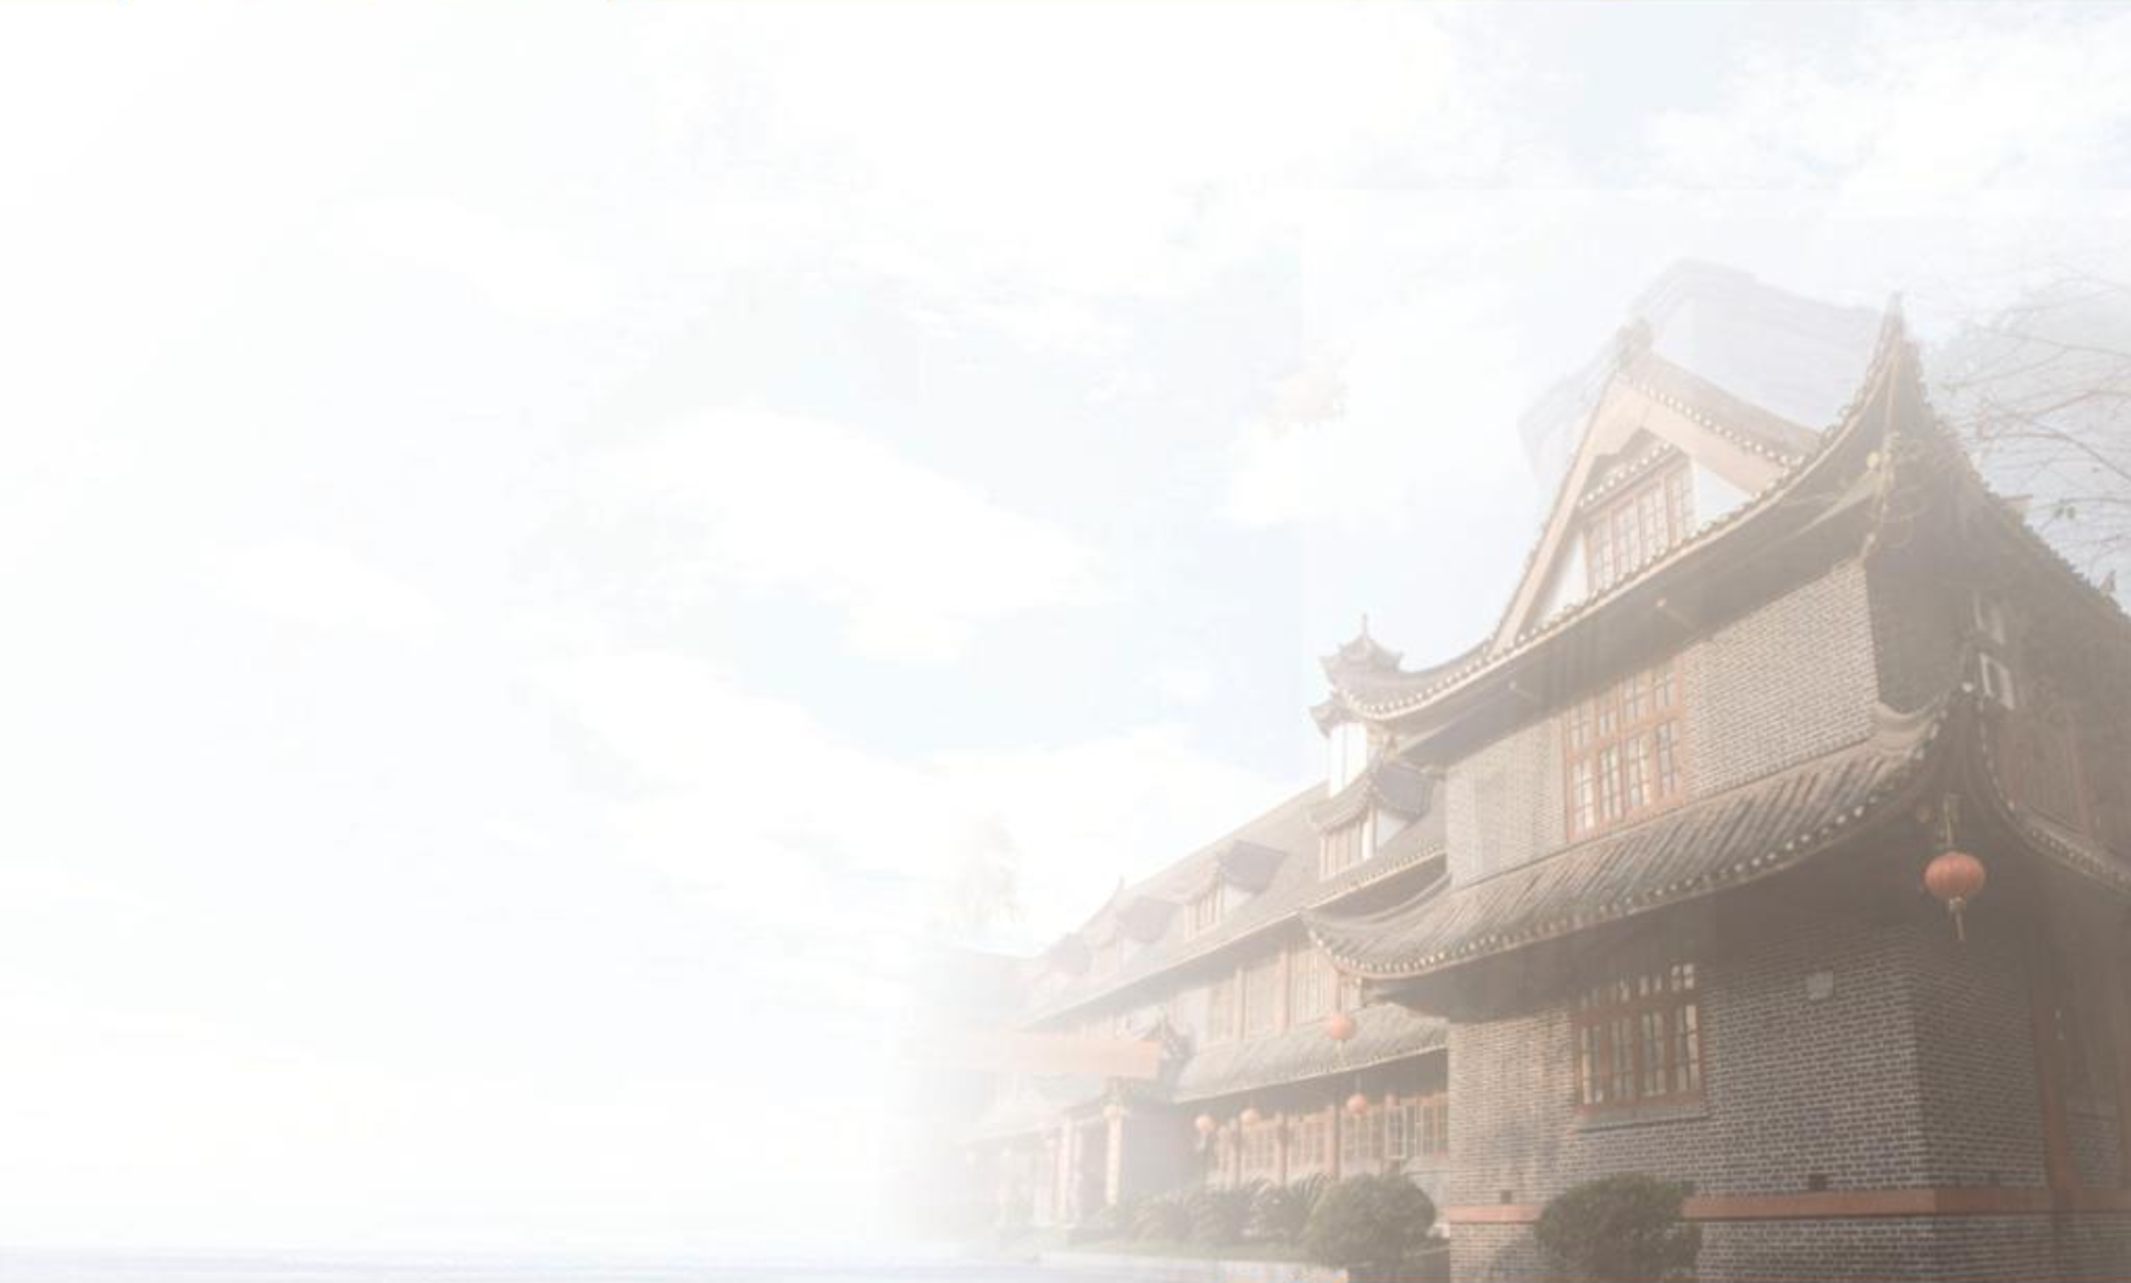
\includegraphics[width=1\paperwidth,height=1\paperheight]{fig/background.pdf}};
\end{tikzpicture}%
}
% other packages
\usepackage{latexsym,amsmath,xcolor,multicol,booktabs,calligra}
\usepackage{graphicx,pstricks,listings,stackengine}
\usepackage{animate}
\usepackage{cqu}
\usepackage{media9}
\newcounter{chapter} % 在这里定义一个 "chapter" 计数器
\usepackage[linesnumbered,ruled,vlined,resetcount,algochapter]{algorithm2e}
\usepackage{dsfont}
\usepackage{mathrsfs}
\usepackage{amsmath}
\usepackage{amssymb}
\usepackage{unicode-math} % 加载unicode-math宏包
\usepackage{cases} % 加载 cases 宏包
\usepackage{lmodern}
%\setmathrm{<正文字体>} % 将数学字体设置为正文字体

% packages and settings for bibtex
\usepackage[backend=bibtex, style=numeric,sorting=none]{biblatex}
\addbibresource{ref.bib}
\setbeamerfont{footnote}{size=\tiny}   % footnote for bibtex

% defs
\def\cmd#1{\texttt{\color{red}\footnotesize $\backslash$#1}}
\def\env#1{\texttt{\color{blue}\footnotesize #1}}
\definecolor{cqublue}{RGB}{2,82,159} % Standard Color-CQU Blue
\definecolor{deepred}{rgb}{0.6,0,0}
\definecolor{deepgreen}{rgb}{0,0.5,0}
\definecolor{halfgray}{gray}{0.55}

\lstset{
    basicstyle=\ttfamily\small,
    keywordstyle=\bfseries\color{cqublue},
    emphstyle=\ttfamily\color{deepred},    % Custom highlighting style
    stringstyle=\color{deepgreen},
    numbers=left,
    numberstyle=\small\color{halfgray},
    rulesepcolor=\color{red!20!green!20!blue!20},
    frame=shadowbox,
}

\setbeamertemplate{bibliography item}[text]   % reference list for bibtex
\setbeamerfont{bibliography item}{family=\rmfamily, size=\footnotesize}
% 设置参考文献内容的字体和字体大小
\renewcommand*{\bibfont}{\scriptsize}

\author[许新操]{{{\color{cqublue}答辩人}:许新操} \qquad {{\color{cqublue}指导教师}:刘凯\ 教授}}
\title{车载信息物理融合系统关键技术研究}
\subtitle{重庆大学博士学位论文答辩}
\institute{重庆大学\ 计算机学院}
%\date[2023] % (optional)
%{2023年5月25日}
\begin{document}

\begin{frame}
\Background
    \titlepage
    \begin{figure}[htpb]
        \begin{center}
     
\includegraphics[width=0.10\linewidth]{fig/Chongqing_University_Logo.pdf}
        \end{center}
    \end{figure}
\end{frame}

\newcommand\newBackground{%
\begin{tikzpicture}[remember picture,overlay]
\node[inner sep=0pt,outer sep=0pt,opacity=0.5]
  at (current page.center){
\includegraphics[width=1\paperwidth,height=1\paperheight]{fig/background3.pdf}};
\end{tikzpicture}%
}

%定义背景
\setbeamertemplate{background}{
\begin{tikzpicture}[remember picture,overlay]
\node[inner sep=0pt,outer sep=0pt,opacity=0.5]
  at (current page.center){
\includegraphics[width=1\paperwidth,height=1\paperheight]{fig/background2.pdf}};
\end{tikzpicture}%
}


% 定义自定义目录页模板
\defbeamertemplate*{custom toc}{custom}{
% 显示目录
\tableofcontents[sectionstyle=show,subsectionstyle=show/shaded/hide,subsubsectionstyle=show/shaded/hide]
}

\begin{frame}
\frametitle{内容提纲}
  \usebeamertemplate{custom toc}
\end{frame}

\section[\englishfont 1 研究背景]{研究背景}
\subsection[\englishfont 1.1 车联网]{1.1 车联网}

\begin{frame}{智能交通系统驱动核心}
\frametitle{\englishfont 智能交通系统驱动核心}
\newBackground
\begin{center}
\begin{textblock*}{\textwidth}(1cm,2cm)
\begin{spacing}{0}
  \small \colorbox{cqublue}{\color{white}{车联网及其所驱动的}}
\end{spacing}
\end{textblock*}
\end{center}

\begin{center}
\begin{textblock*}{\textwidth}(1cm,2.5cm)
\begin{spacing}{0}
  \small \colorbox{cqublue}{\color{white}{智能交通与智慧城市}}
\end{spacing}
\end{textblock*}
\end{center}

\begin{center}
\begin{textblock*}{\textwidth}(1cm,6.5cm)
\begin{spacing}{0}
  \small \colorbox{cqublue}{\color{white}{推动汽车向}\color{yellow}{网联化、智}}
\end{spacing}
\end{textblock*}
\end{center}

\begin{center}
\begin{textblock*}{\textwidth}(1cm,7cm)
\begin{spacing}{0}
  \small \colorbox{cqublue}{\color{yellow}{能化与协同化}\color{white}{方向演进}}
\end{spacing}
\end{textblock*}
\end{center}

\begin{center}
\begin{textblock*}{\textwidth}(-4cm,1.6cm)
\animategraphics[width=0.28\textwidth,autoplay,loop]{30}{fig/v2x1/v2x1-}{0}{95}\\ \footnotesize 车载移动通信\\
\scriptsize 高移动性 \hspace{1em} 高动态拓扑
\end{textblock*}
\end{center}

\begin{center}
\begin{textblock*}{\textwidth}(6cm,1.6cm)
\animategraphics[width=0.28\textwidth,autoplay,loop]{1}{fig/v2x2/v2x2-}{0}{2}\\ \footnotesize 人车路协同\\
\scriptsize 低时延 \hspace{1em} 分布式 \hspace{1em} 高异构
\end{textblock*}
\end{center}
  
  \begin{center}
  	\begin{figure}
  		\begin{textblock*}{\textwidth}(1cm,3.5cm)
    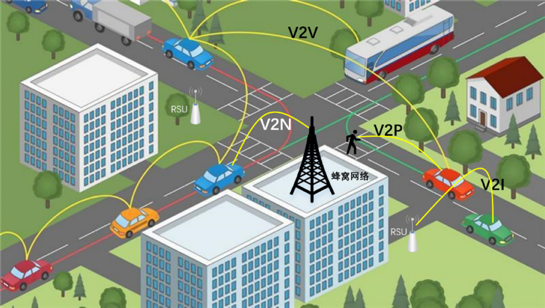
\includegraphics[width=0.35\textwidth]{fig/v2x.pdf}
  		\end{textblock*}
	\end{figure}
  \end{center}
  
\begin{center}
\begin{textblock*}{\textwidth}(-4cm,5cm)
\animategraphics[width=0.28\textwidth,autoplay,loop]{10}{fig/v2x3/v2x3-}{0}{20}\\\footnotesize 计算卸载与优化\\
\scriptsize 复杂任务 \hspace{1em} 多样性应用
\end{textblock*}
\end{center}

\begin{center}
\begin{textblock*}{\textwidth}(6cm,5cm)
\animategraphics[width=0.28\textwidth,autoplay,loop]{12}{fig/v2x4/v2x4-}{0}{24}\\ \footnotesize 智能交通系统\\
\scriptsize 碰撞预警 \hspace{1em} 自动驾驶
\end{textblock*}
\end{center}
\end{frame}

\begin{frame}{国家战略}
\frametitle{\englishfont 国家战略}
\newBackground
\begin{center}
\begin{textblock*}{\textwidth}(0.2cm,1.6cm)
\begin{figure}
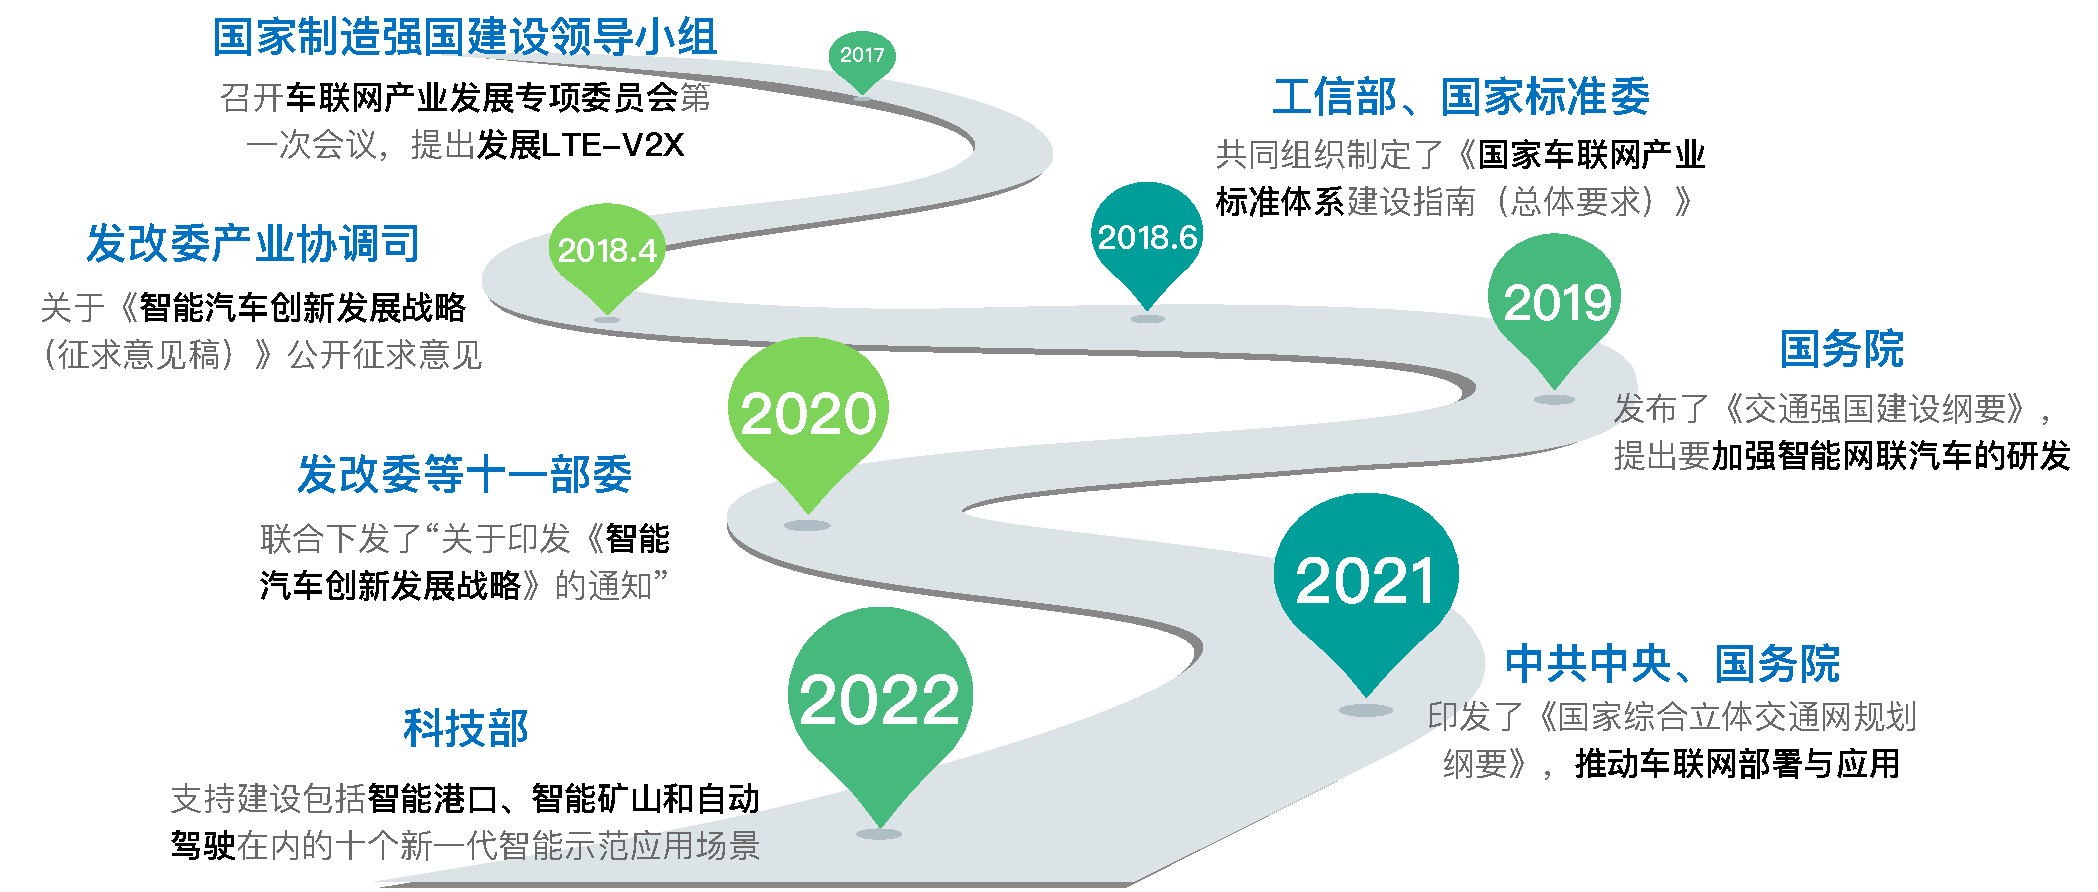
\includegraphics[width=1.1\textwidth]{fig/policy.pdf}
\end{figure}
\end{textblock*}
\end{center}
\end{frame}

\begin{frame}{V2X车联网}
\frametitle{\englishfont V2X车联网}
\newBackground
\begin{center}
\begin{textblock*}{\textwidth}(0.5cm,1.8cm)
\begin{figure}
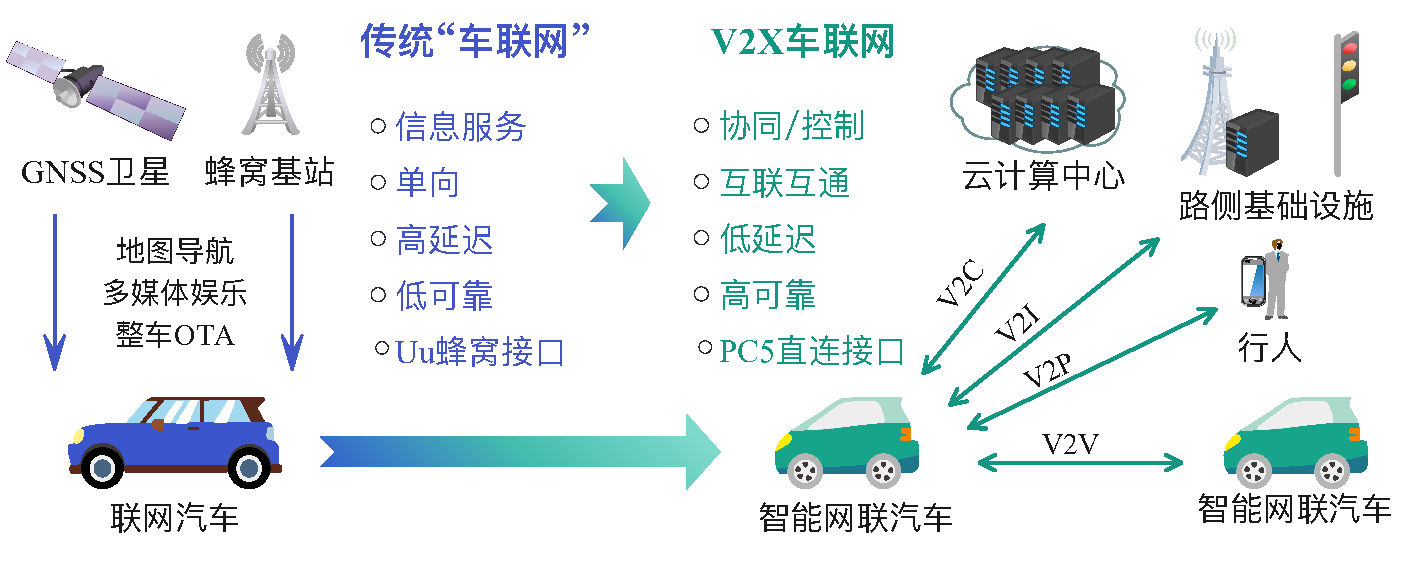
\includegraphics[width=1.1\textwidth]{fig/v2x-evolution.pdf}
\end{figure}
\end{textblock*}
\end{center}
\end{frame}

\subsection[\englishfont 1.2 车载信息物理融合系统]{1.2 车载信息物理融合系统}
\begin{frame}{车载信息物理融合系统}
\frametitle{\englishfont 车载信息物理融合系统 (Vehicular Cyber-Physical Systems, VCPS)}
\newBackground
\begin{center}
\begin{textblock*}{\textwidth}(1cm,1.8cm)
\begin{itemize} \englishfont
	\item[\ding{111}] {\color{cqublue}{关键思想}}
	\begin{itemize}
	\begin{footnotesize}
		\item[\ding{226}] 集成{\color{cqublue}{感知、计算、通信与控制}}技术
		\item[\ding{226}] 构建{\color{cqublue}{物理}}世界与{\color{cqublue}{虚拟}}世界的相互{\color{cqublue}{映射}}
	\end{footnotesize}
	\end{itemize}
	\item[\ding{111}]  {\color{cqublue}{发展历程}}
	\begin{itemize}
	\begin{footnotesize}
		\item[\ding{226}] 2006年,美国NSF启动CPS研究计划
		\item[\ding{226}] 2011年,LI等人首次将CPS引入车联网
	\end{footnotesize}
	\end{itemize}
\end{itemize}
\end{textblock*}
\end{center}

\begin{center}
\begin{textblock*}{\textwidth}(-2cm,5.2cm)
\begin{figure}
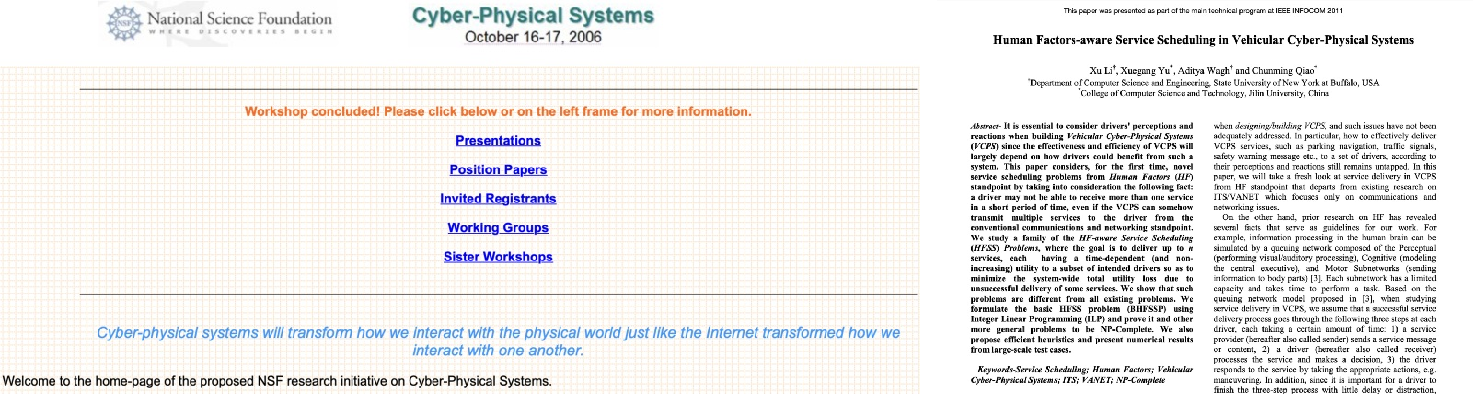
\includegraphics[width=0.6\textwidth]{fig/vcps_nsf.pdf}
\end{figure}
\end{textblock*}
\end{center}

\begin{center}
\begin{textblock*}{\textwidth}(5.5cm,1.8cm)
\begin{figure}
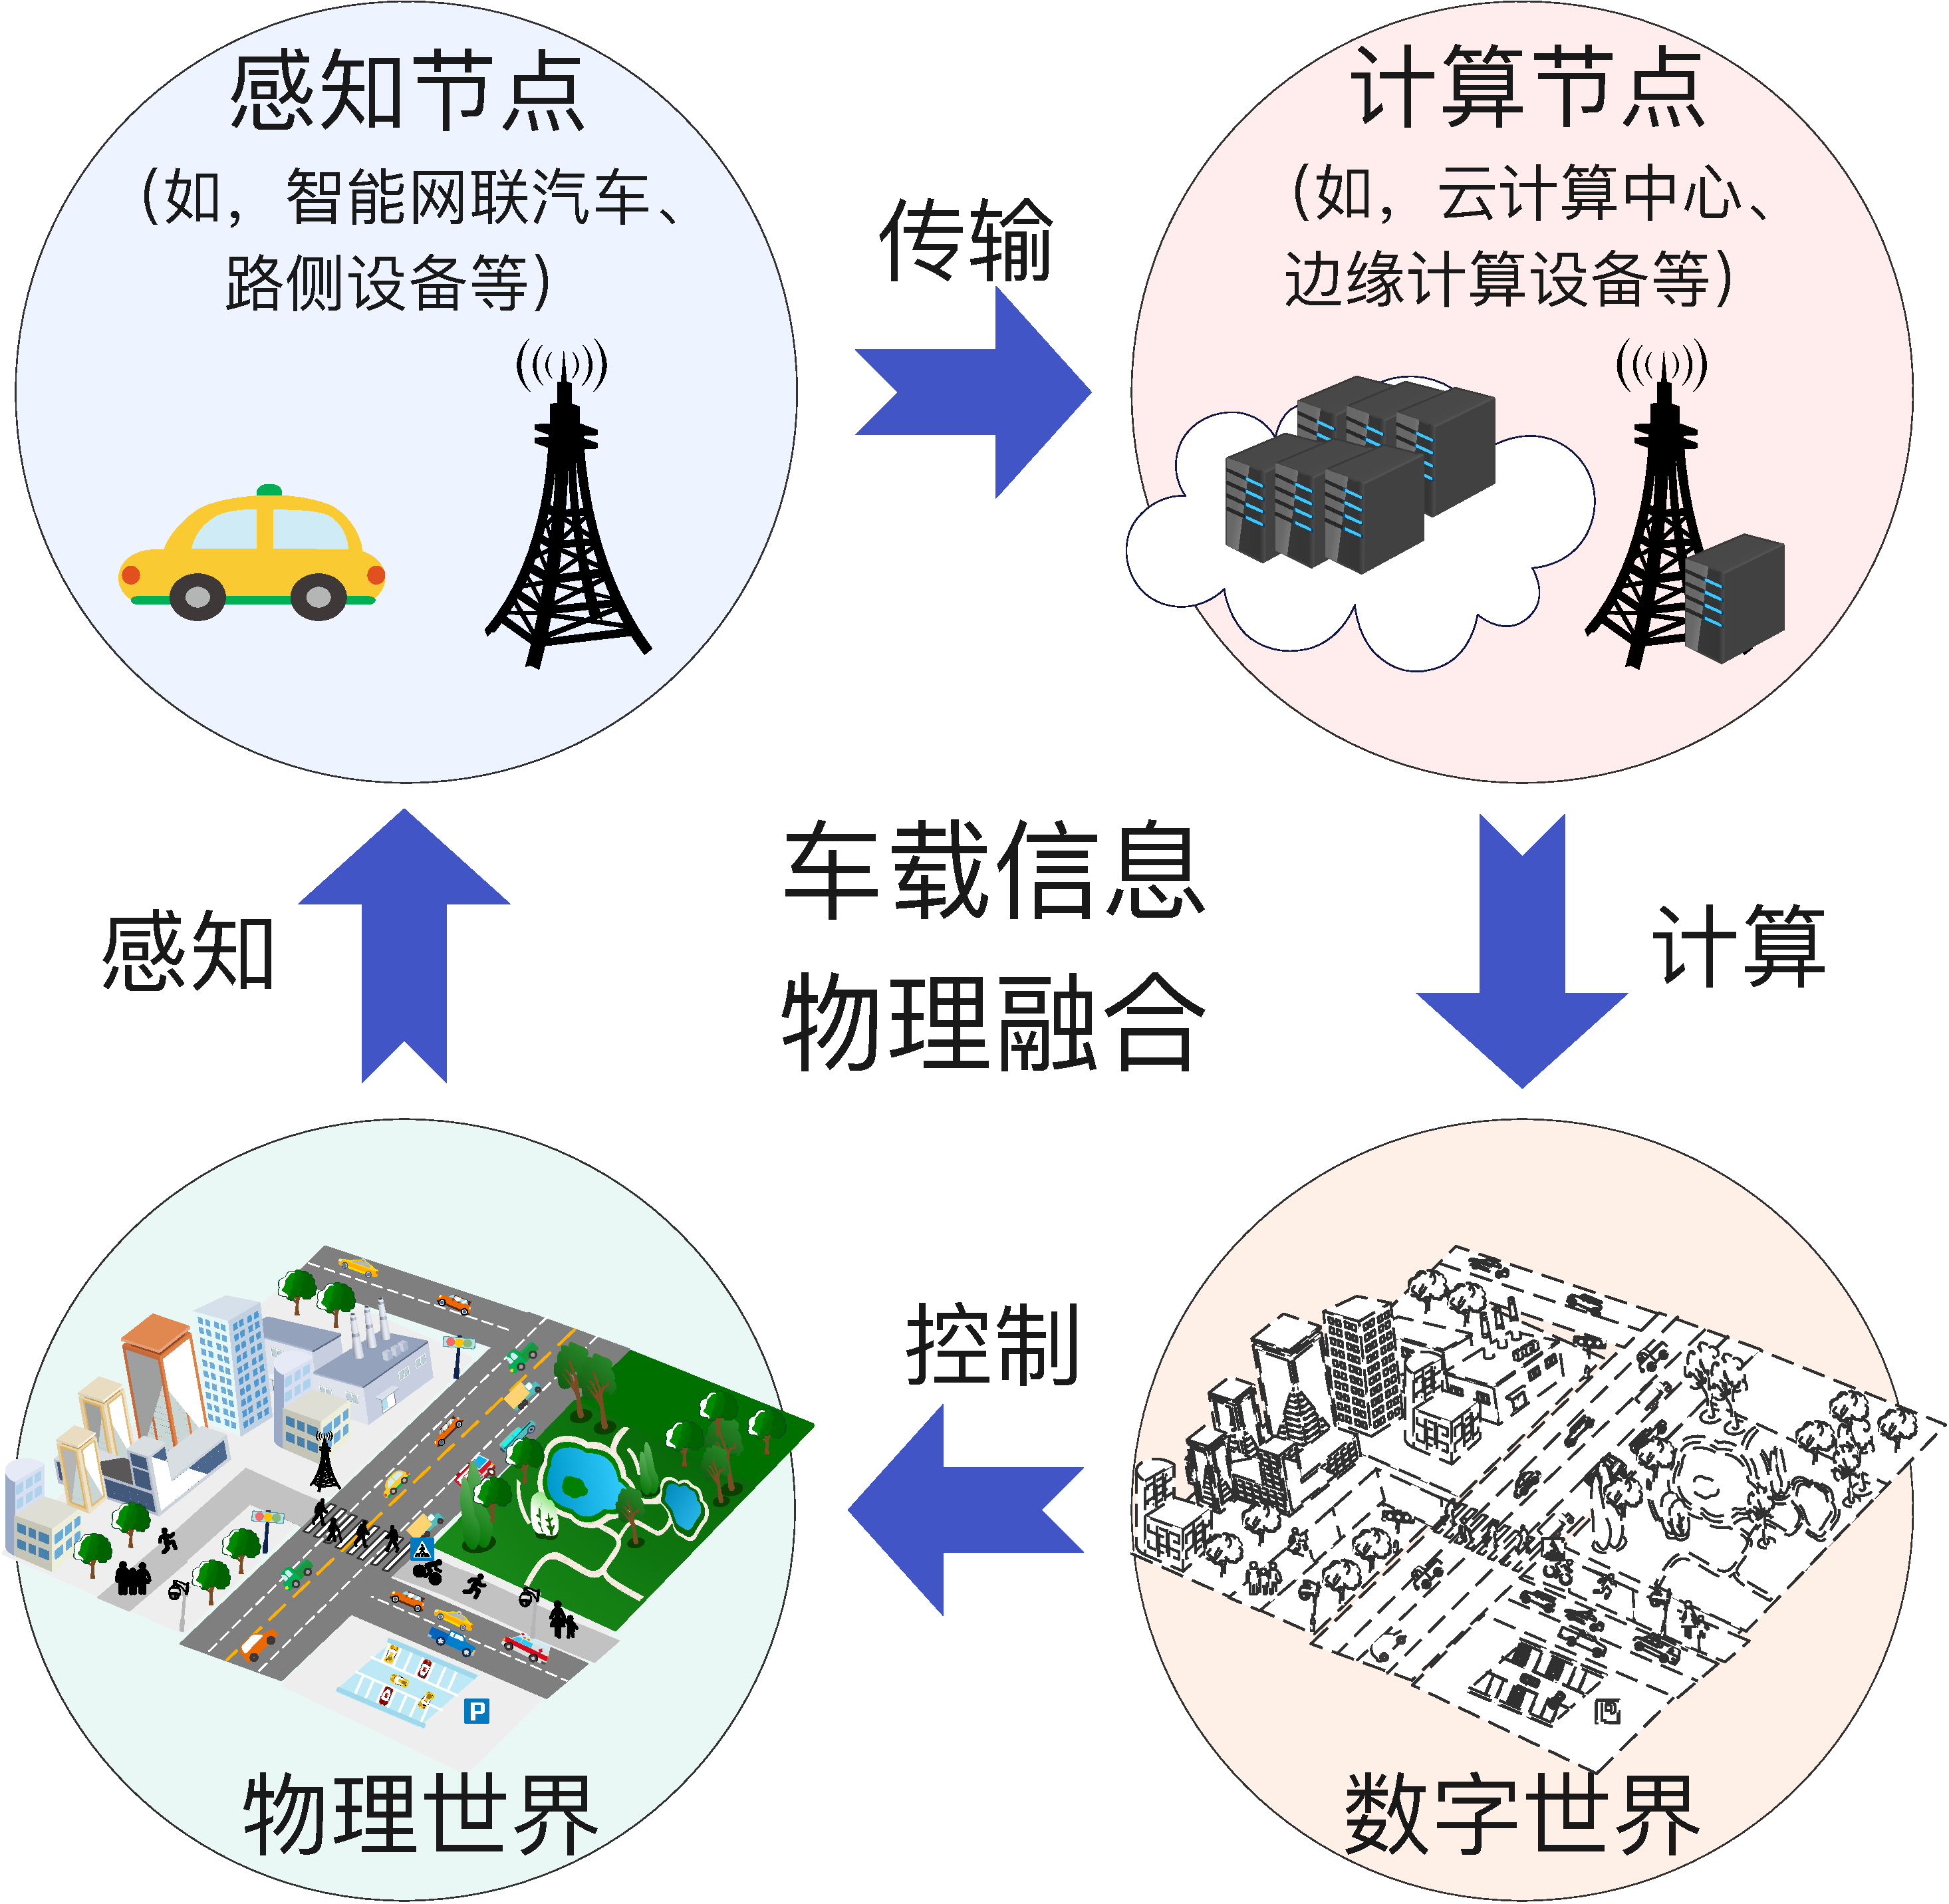
\includegraphics[width=0.45\textwidth]{fig/vcps.pdf}
\end{figure}
\end{textblock*}
\end{center}
\end{frame}

\begin{frame}{问题与挑战}
\frametitle{\englishfont 问题与挑战}
\newBackground
\begin{center}
\begin{textblock*}{\textwidth}(1cm,1.65cm)
\begin{figure}
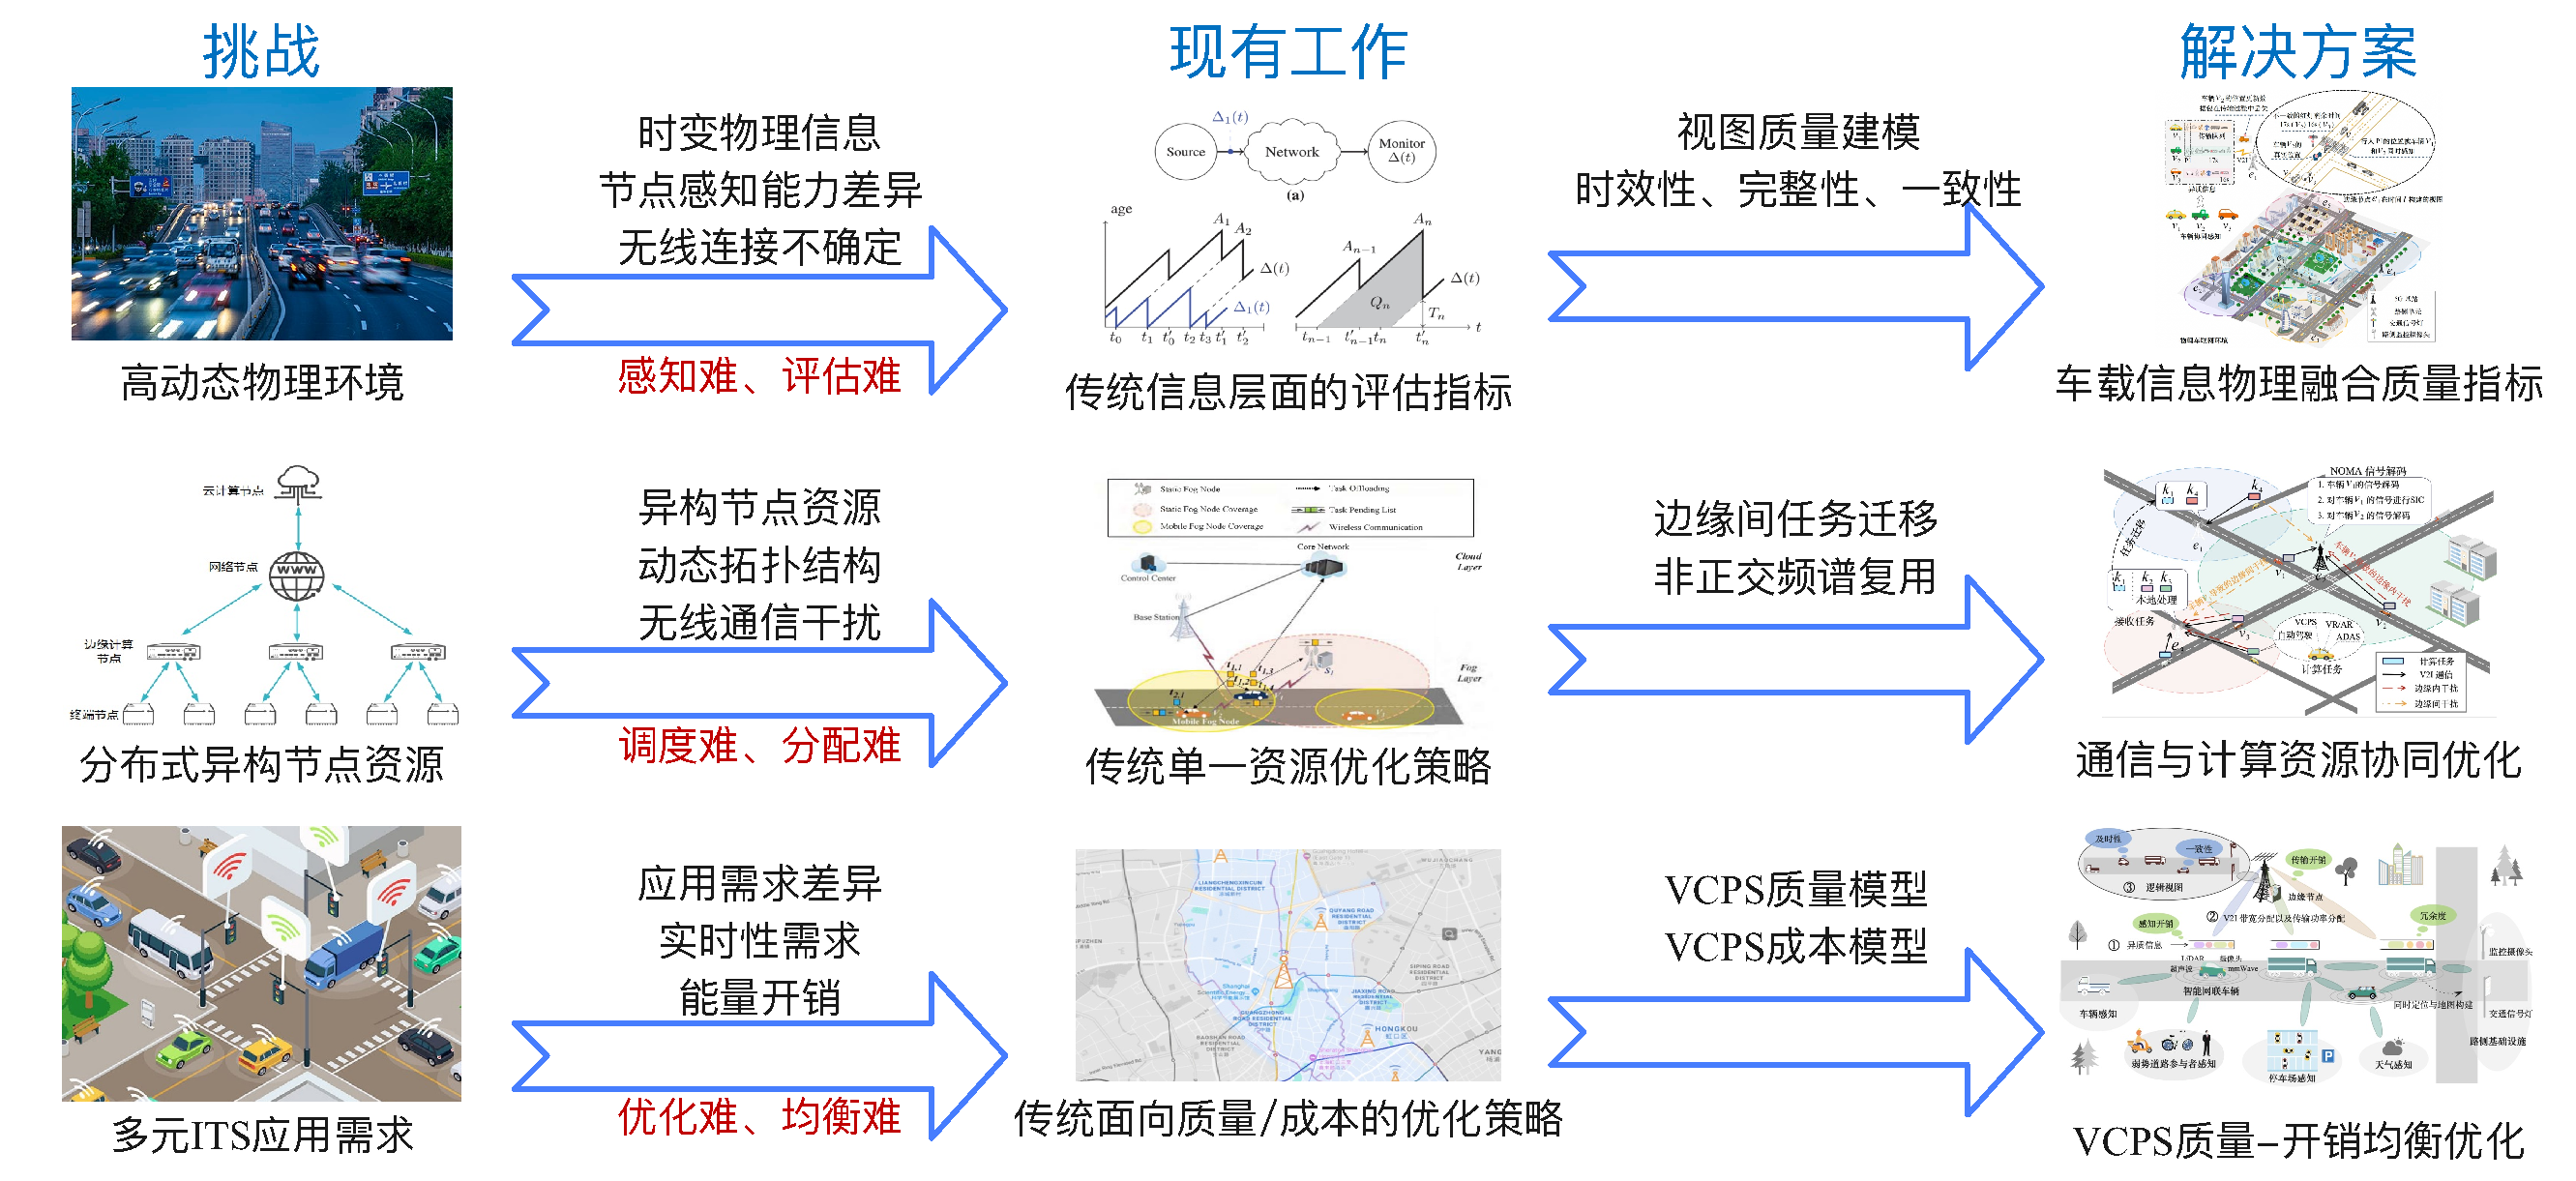
\includegraphics[width=1\textwidth]{fig/challenges.pdf}
\end{figure}
\end{textblock*}
\end{center}
\end{frame}


\begin{frame}{主要研究内容}
\frametitle{\englishfont 主要研究内容}
\newBackground
\begin{center}
\begin{textblock*}{\textwidth}(1cm,1.65cm)
\begin{figure}
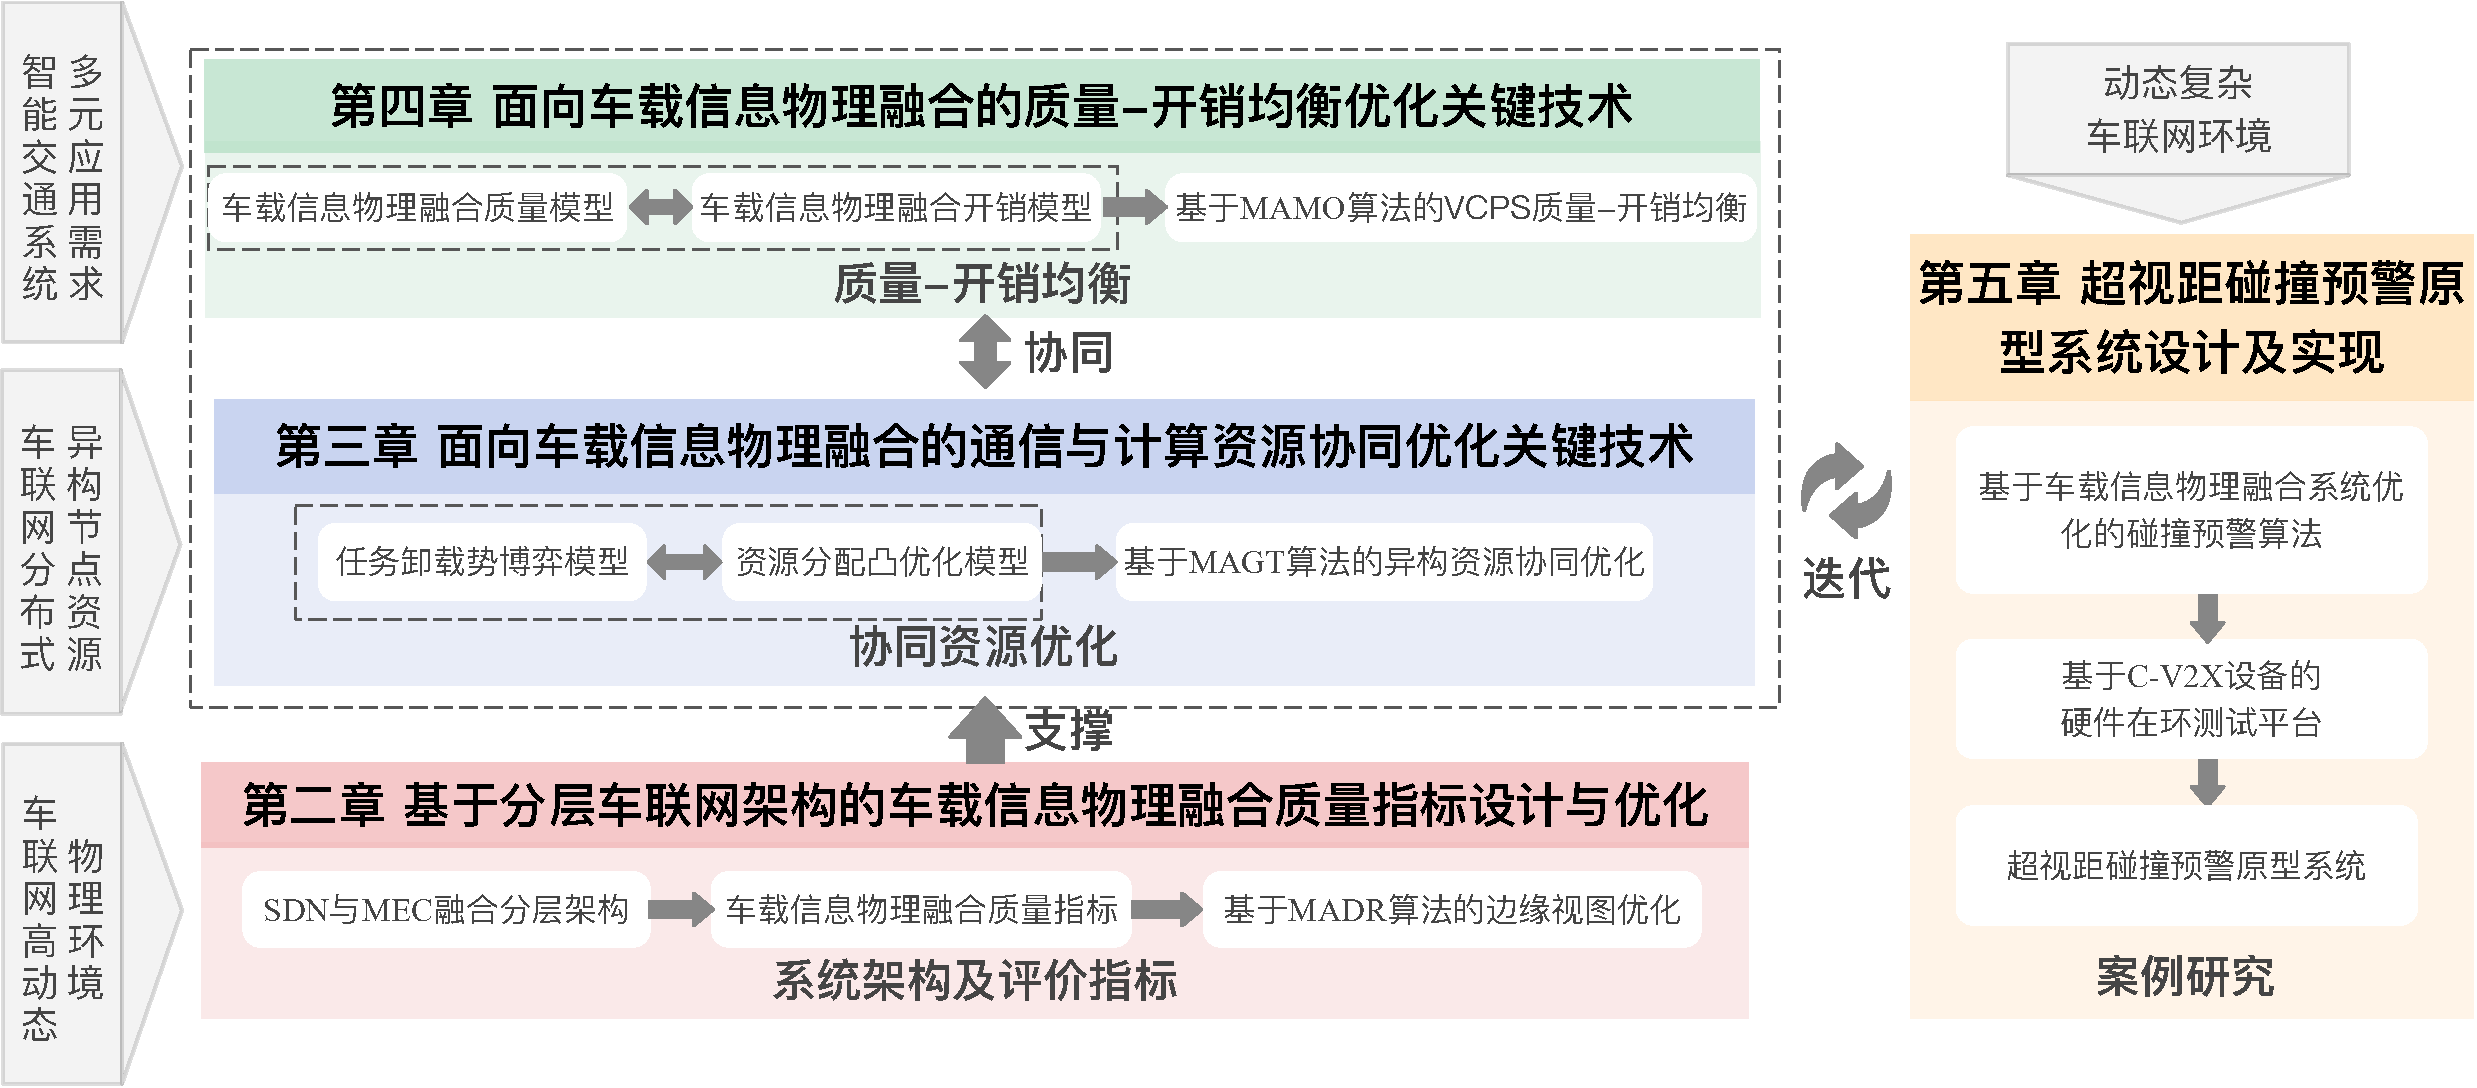
\includegraphics[width=1.05\textwidth]{fig/research_content.pdf}
\end{figure}
\end{textblock*}
\end{center}
\end{frame}
\section[\englishfont 2 研究内容及贡献]{研究内容及贡献}

\subsection[\englishfont 2.1 基于分层车联网架构的车载信息物理融合质量指标设计与优化]{2.1 基于分层车联网架构的车载信息物理融合质量指标设计与优化}

\begin{frame}{研究贡献}
\newBackground
\begin{center}
\begin{textblock*}{\textwidth}(-1cm,1.8cm)
  \small \englishfont \colorbox{cqublue}{\color{white}{创新的服务架构和高效的数据感知与质量}}
\end{textblock*}
\end{center}

\begin{center}
\begin{textblock*}{\textwidth}(-1cm,2.3cm)
  \small \englishfont \colorbox{cqublue}{\color{white}{评估模型是 VCPS的{\color{yellow}{架构基础}}与{\color{yellow}{驱动核心}}}}
\end{textblock*}
\end{center}

\begin{center}
\begin{textblock*}{\textwidth}(-1.8cm,3.16cm)
\begin{minipage}[t]{0.7\textwidth}
\begin{itemize}[itemsep=0.2\baselineskip] \englishfont
	\item[\ding{111}] {{\color{cqublue}{\textbf{架构}}}:{\color{red}{SDN+MEC}}车联网分层架构}
	\item[\ding{111}]  {{\color{cqublue}{\textbf{指标}}}:{\color{red}{Age of View}}评估逻辑视图质量}
		\begin{itemize}[itemsep=0.2\baselineskip] 
		\begin{small}
		\item[\ding{226}] 时效性、完整性、一致性
		\item[\ding{226}] 最大化VCPS质量问题
		\end{small}
		\end{itemize}
	\item[\ding{111}]  {{\color{cqublue}{\textbf{算法}}}:基于差分奖励的多智能体强化学习 ({\color{red}{MADR}})}
	\item[\ding{111}]  {{\color{cqublue}{\textbf{实验}}}:有效提高车载信息物理融合质量}
\end{itemize}
\end{minipage}
\end{textblock*}
\end{center}

\begin{center}
\begin{textblock*}{\textwidth}(-1cm,6.7cm)
\fbox{\begin{minipage}[t]{0.78\textwidth}\englishfont \tiny [1] LIU K, \underline{\textcolor{cqublue}{\textbf{XU X}}},  et al. \textcolor{cqublue}{A hierarchical architecture for the future Internet of Vehicles}[J].IEEE Communications Magazine (\textcolor{red}{ComMag}), 2019, 57(7): 41-47. 影响因子: 9.03(2021), 10.892(5年) (中科院SCI 1区)
\end{minipage}}
\fbox{\begin{minipage}[t]{0.78\textwidth}\englishfont \tiny [2] \underline{\textcolor{cqublue}{\textbf{XU X}}}, LIU K, et al. \textcolor{cqublue}{Cooperative sensing and heterogeneous information fusion in VCPS: A multi-agent deep reinforcement learning approach}[J]. IEEE Transactions on Intelligent Transportation Systems (\textcolor{red}{T-ITS}), under major revision. (中科院SCI 1区)
\end{minipage}}
\end{textblock*}
\end{center}

\begin{center}
\begin{textblock*}{\textwidth}(7cm,1.8cm)
\begin{figure}
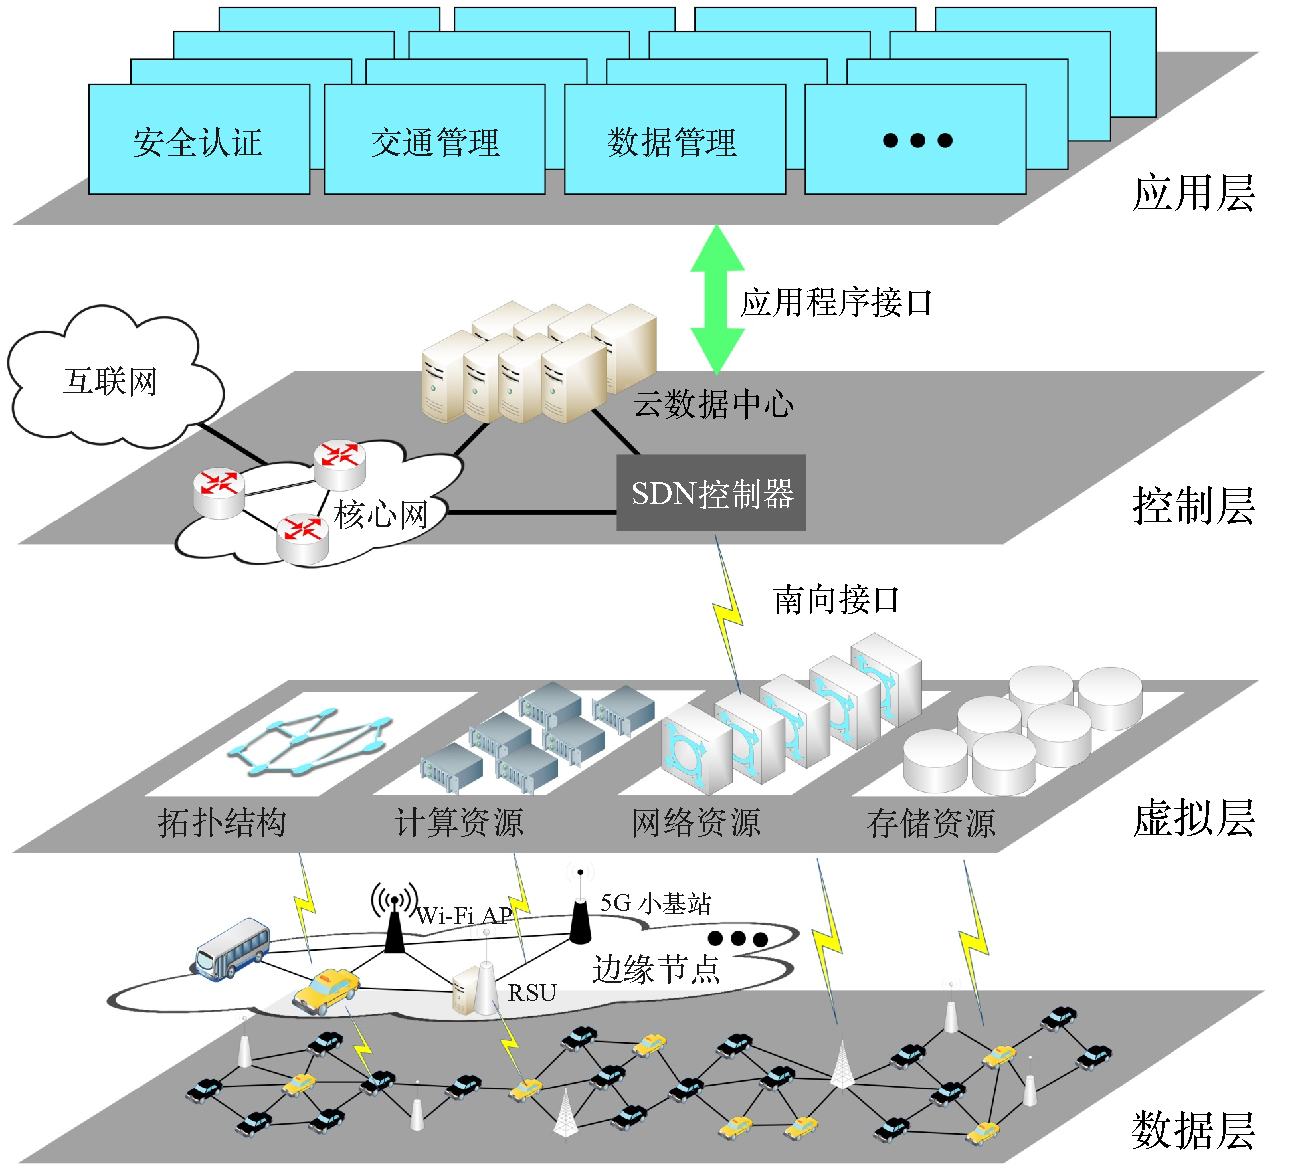
\includegraphics[width=0.23\textwidth]{fig/Fig2-1-hierarchical-architecture.pdf}
\end{figure}
\begin{figure}
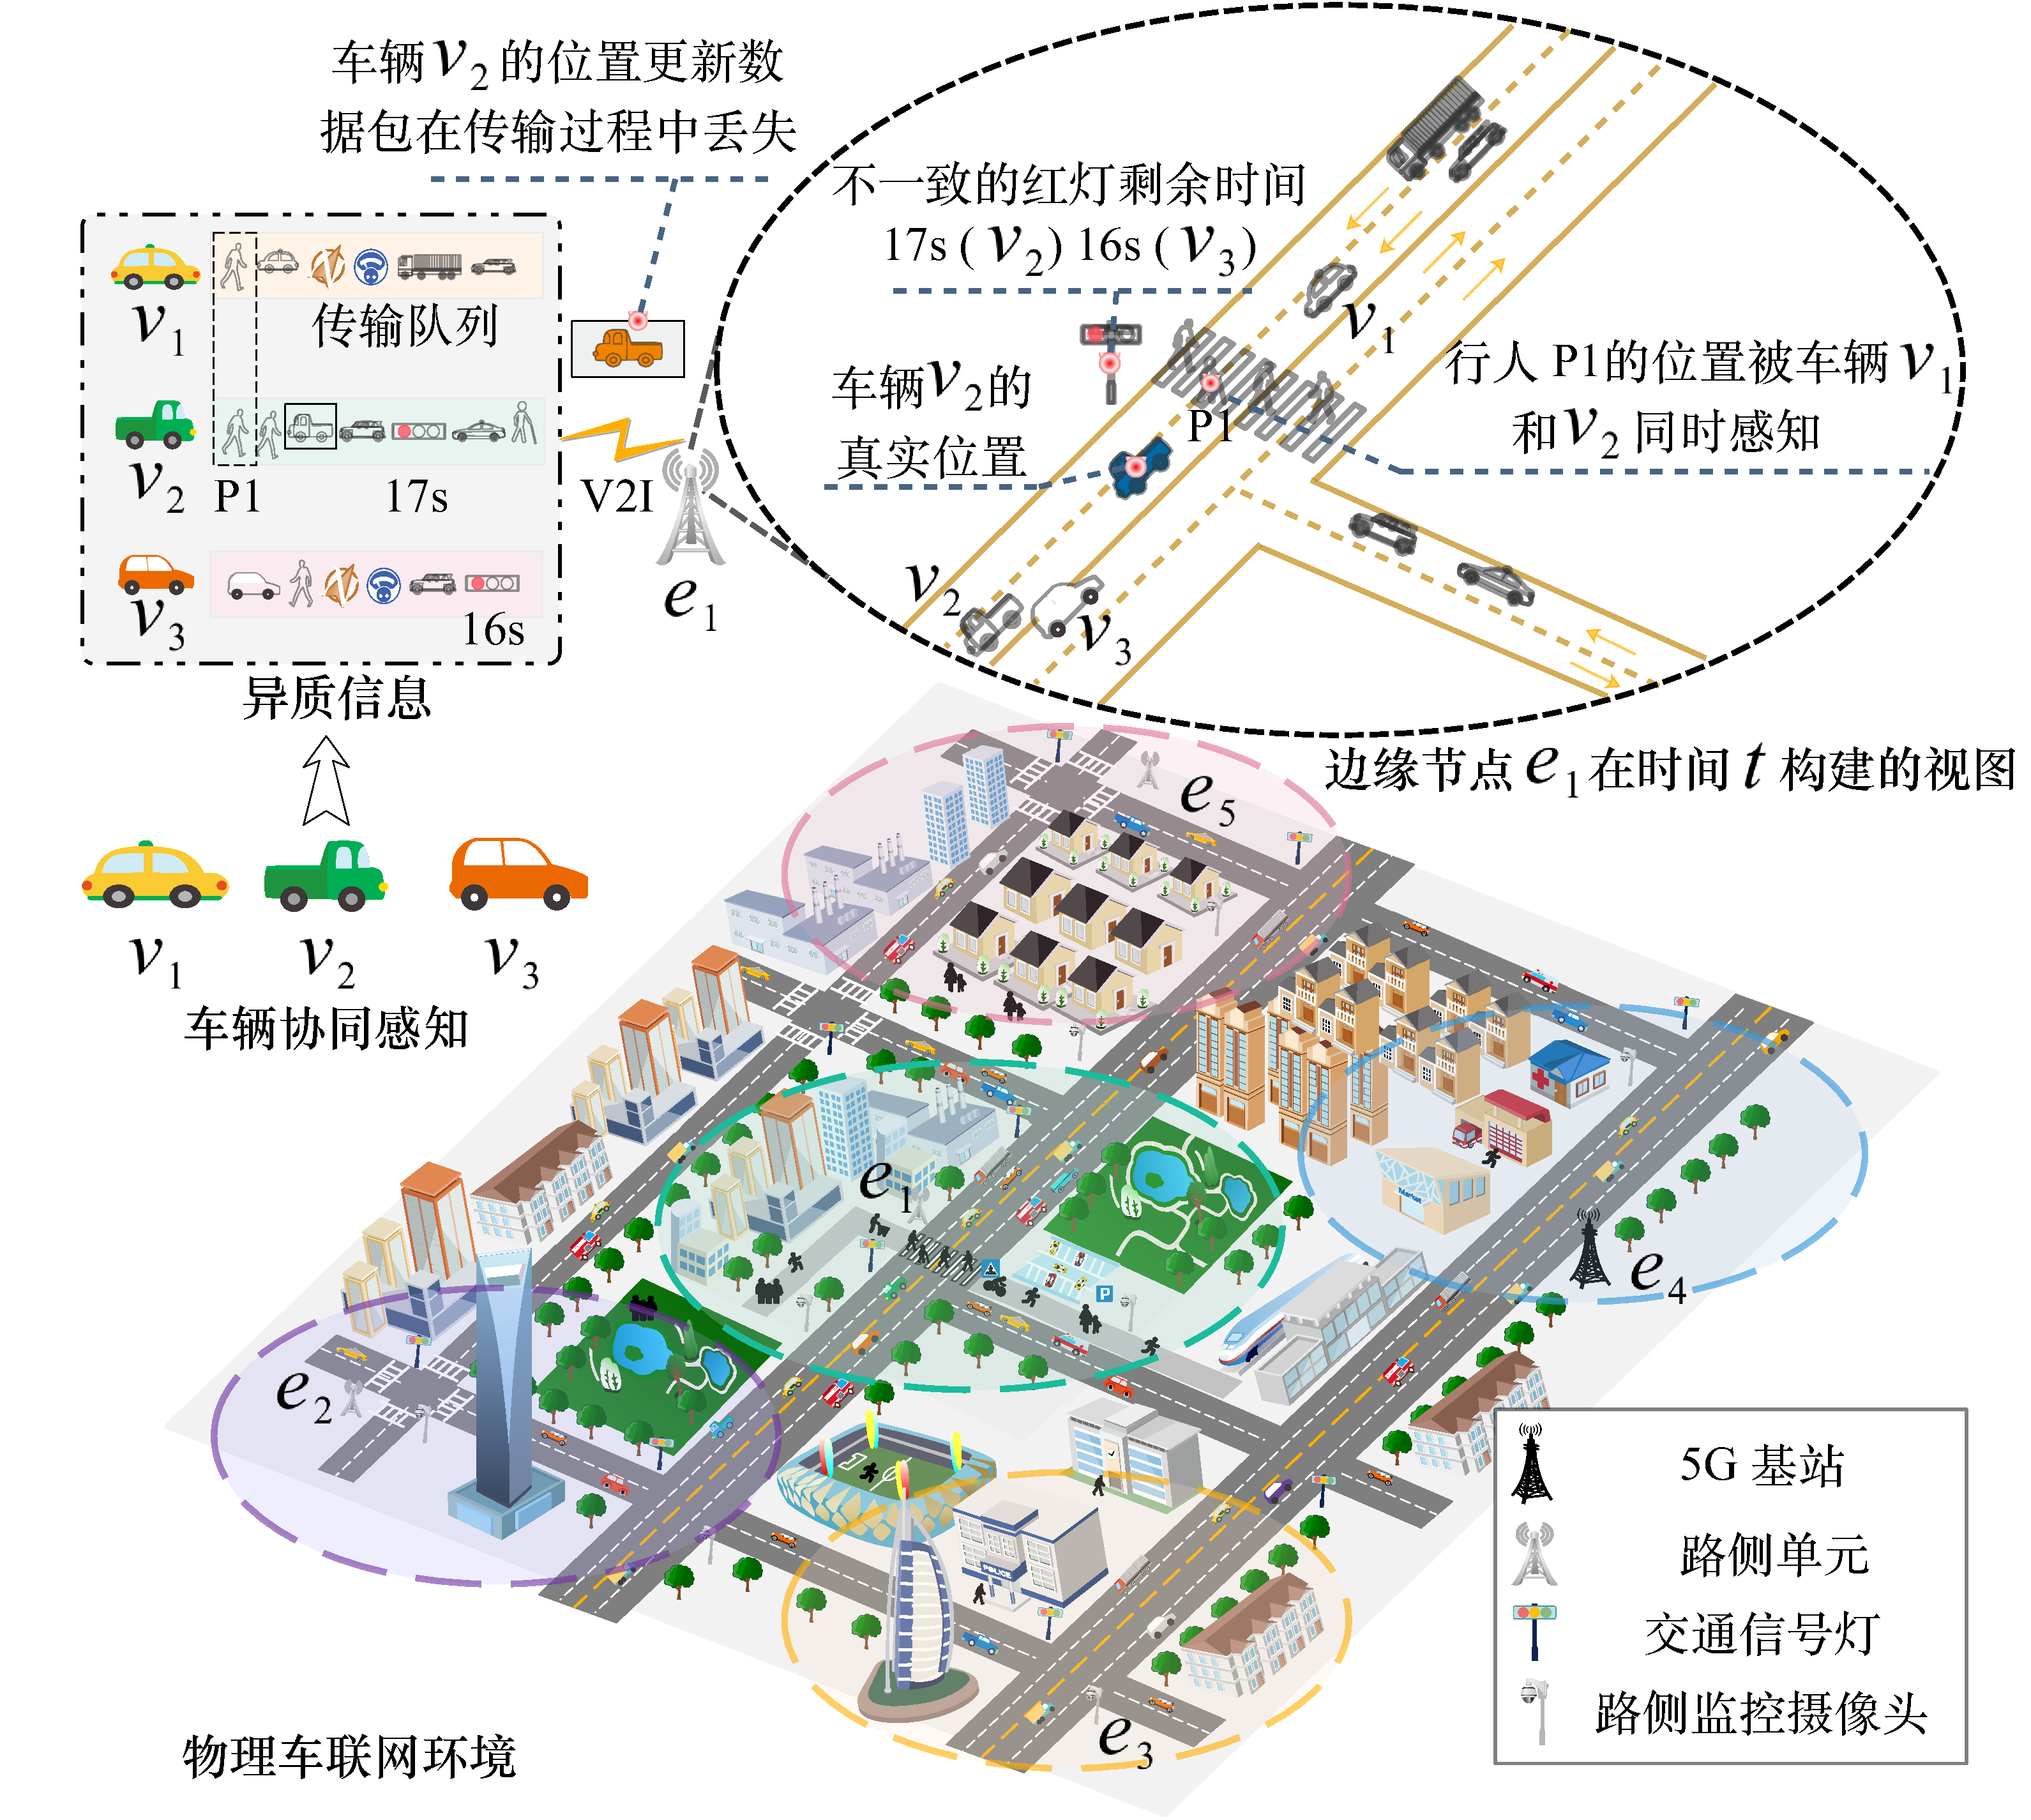
\includegraphics[width=0.23\textwidth]{fig/Fig2-2a-architerture.pdf}
\end{figure}
\end{textblock*}
\end{center}
\end{frame}

\begin{frame}
\frametitle{\englishfont \underline{架构}:车联网分层服务架构}
\newBackground
\begin{center}
\begin{textblock*}{\textwidth}(0.5cm,2.5cm)
\begin{itemize}[itemsep=0.2\baselineskip]  \englishfont
	\item[\ding{111}] {\color{cqublue}{{软件定义网络 ({\color{cqublue}{SDN}})+移动边缘计算 ({\color{cqublue}{MEC}})}}}
	\begin{itemize}[itemsep=0.2\baselineskip] 
	\begin{small}
		\item[\ding{226}] SDN逻辑上集中控制
		\item[\ding{226}] MEC分布式服务
	\end{small}
	\end{itemize}
	\item[\ding{111}]  {\color{cqublue}{分层服务架构}}
	\begin{itemize}[itemsep=0.2\baselineskip] 
	\begin{small}
		\item[\ding{226}] \underline{应用层}:面向业务需求的应用
		\item[\ding{226}] \underline{控制层}:网络功能集中控制
		\item[\ding{226}] \underline{虚拟层}:抽象计算、网络和存储资源
		\item[\ding{226}] \underline{数据层}:存储、处理数据
		\item 
	\end{small} 
	\end{itemize}
\end{itemize}
\end{textblock*}
\end{center}

\begin{center}
\begin{textblock*}{\textwidth}(5.2cm,1.8cm)
\begin{figure}
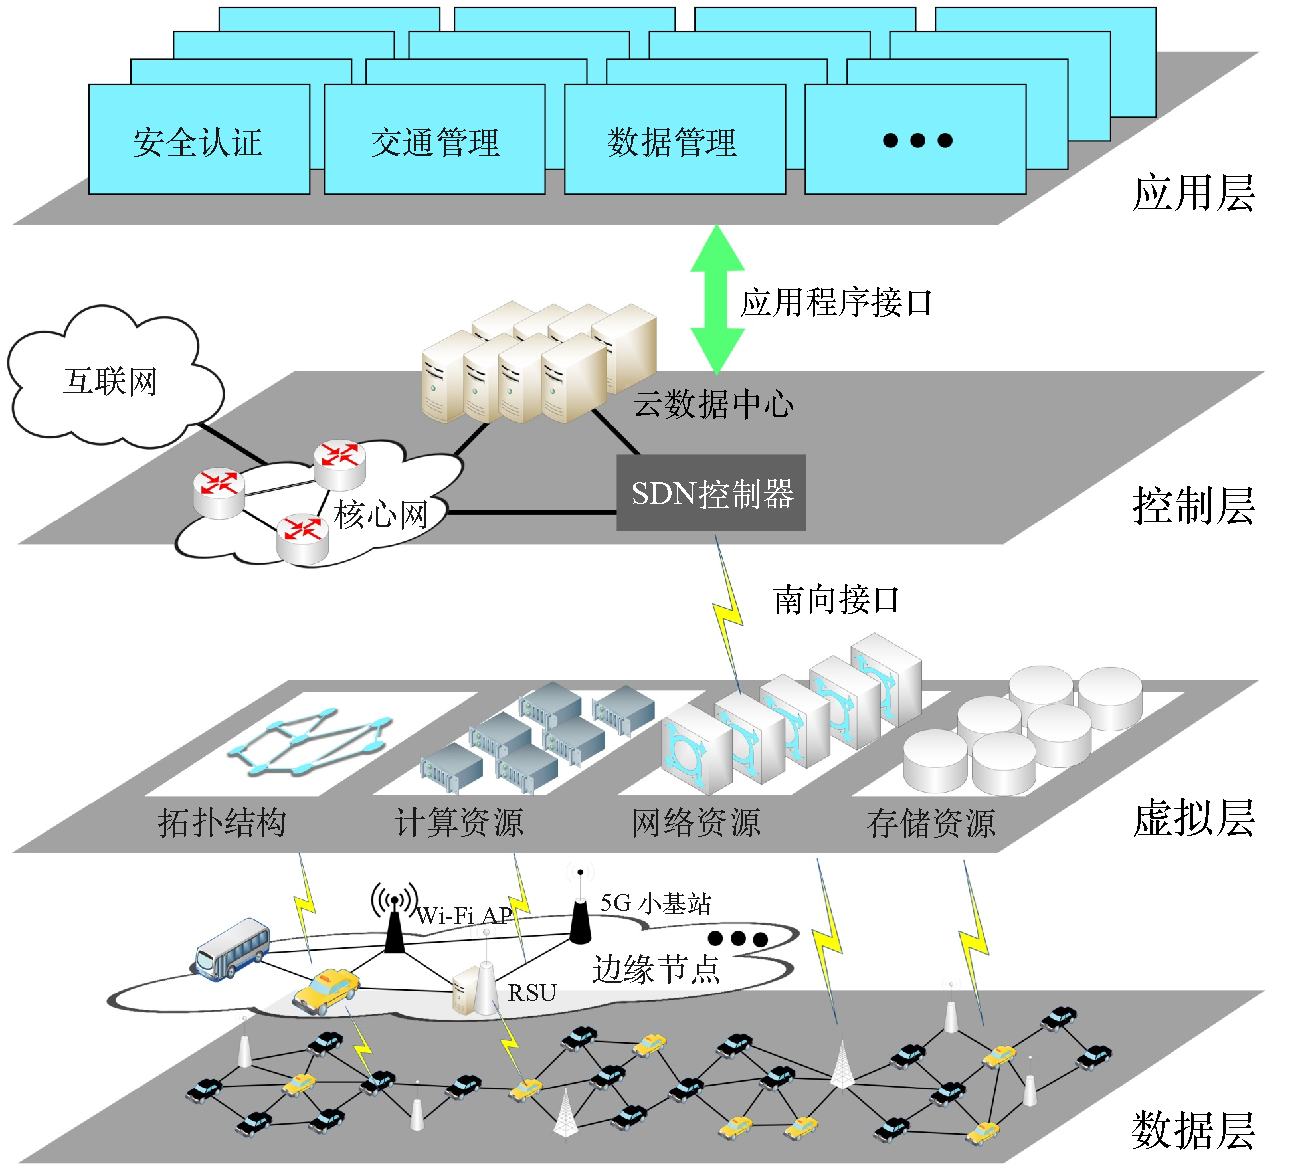
\includegraphics[width=0.47\textwidth]{fig/Fig2-1-hierarchical-architecture.pdf}
\end{figure}
\end{textblock*}
\end{center}
\end{frame}

\begin{frame}
\frametitle{\underline{指标}:感知与信息融合场景}
\newBackground
\begin{center}
\begin{textblock*}{\textwidth}(5.2cm,1.8cm)
\begin{figure}
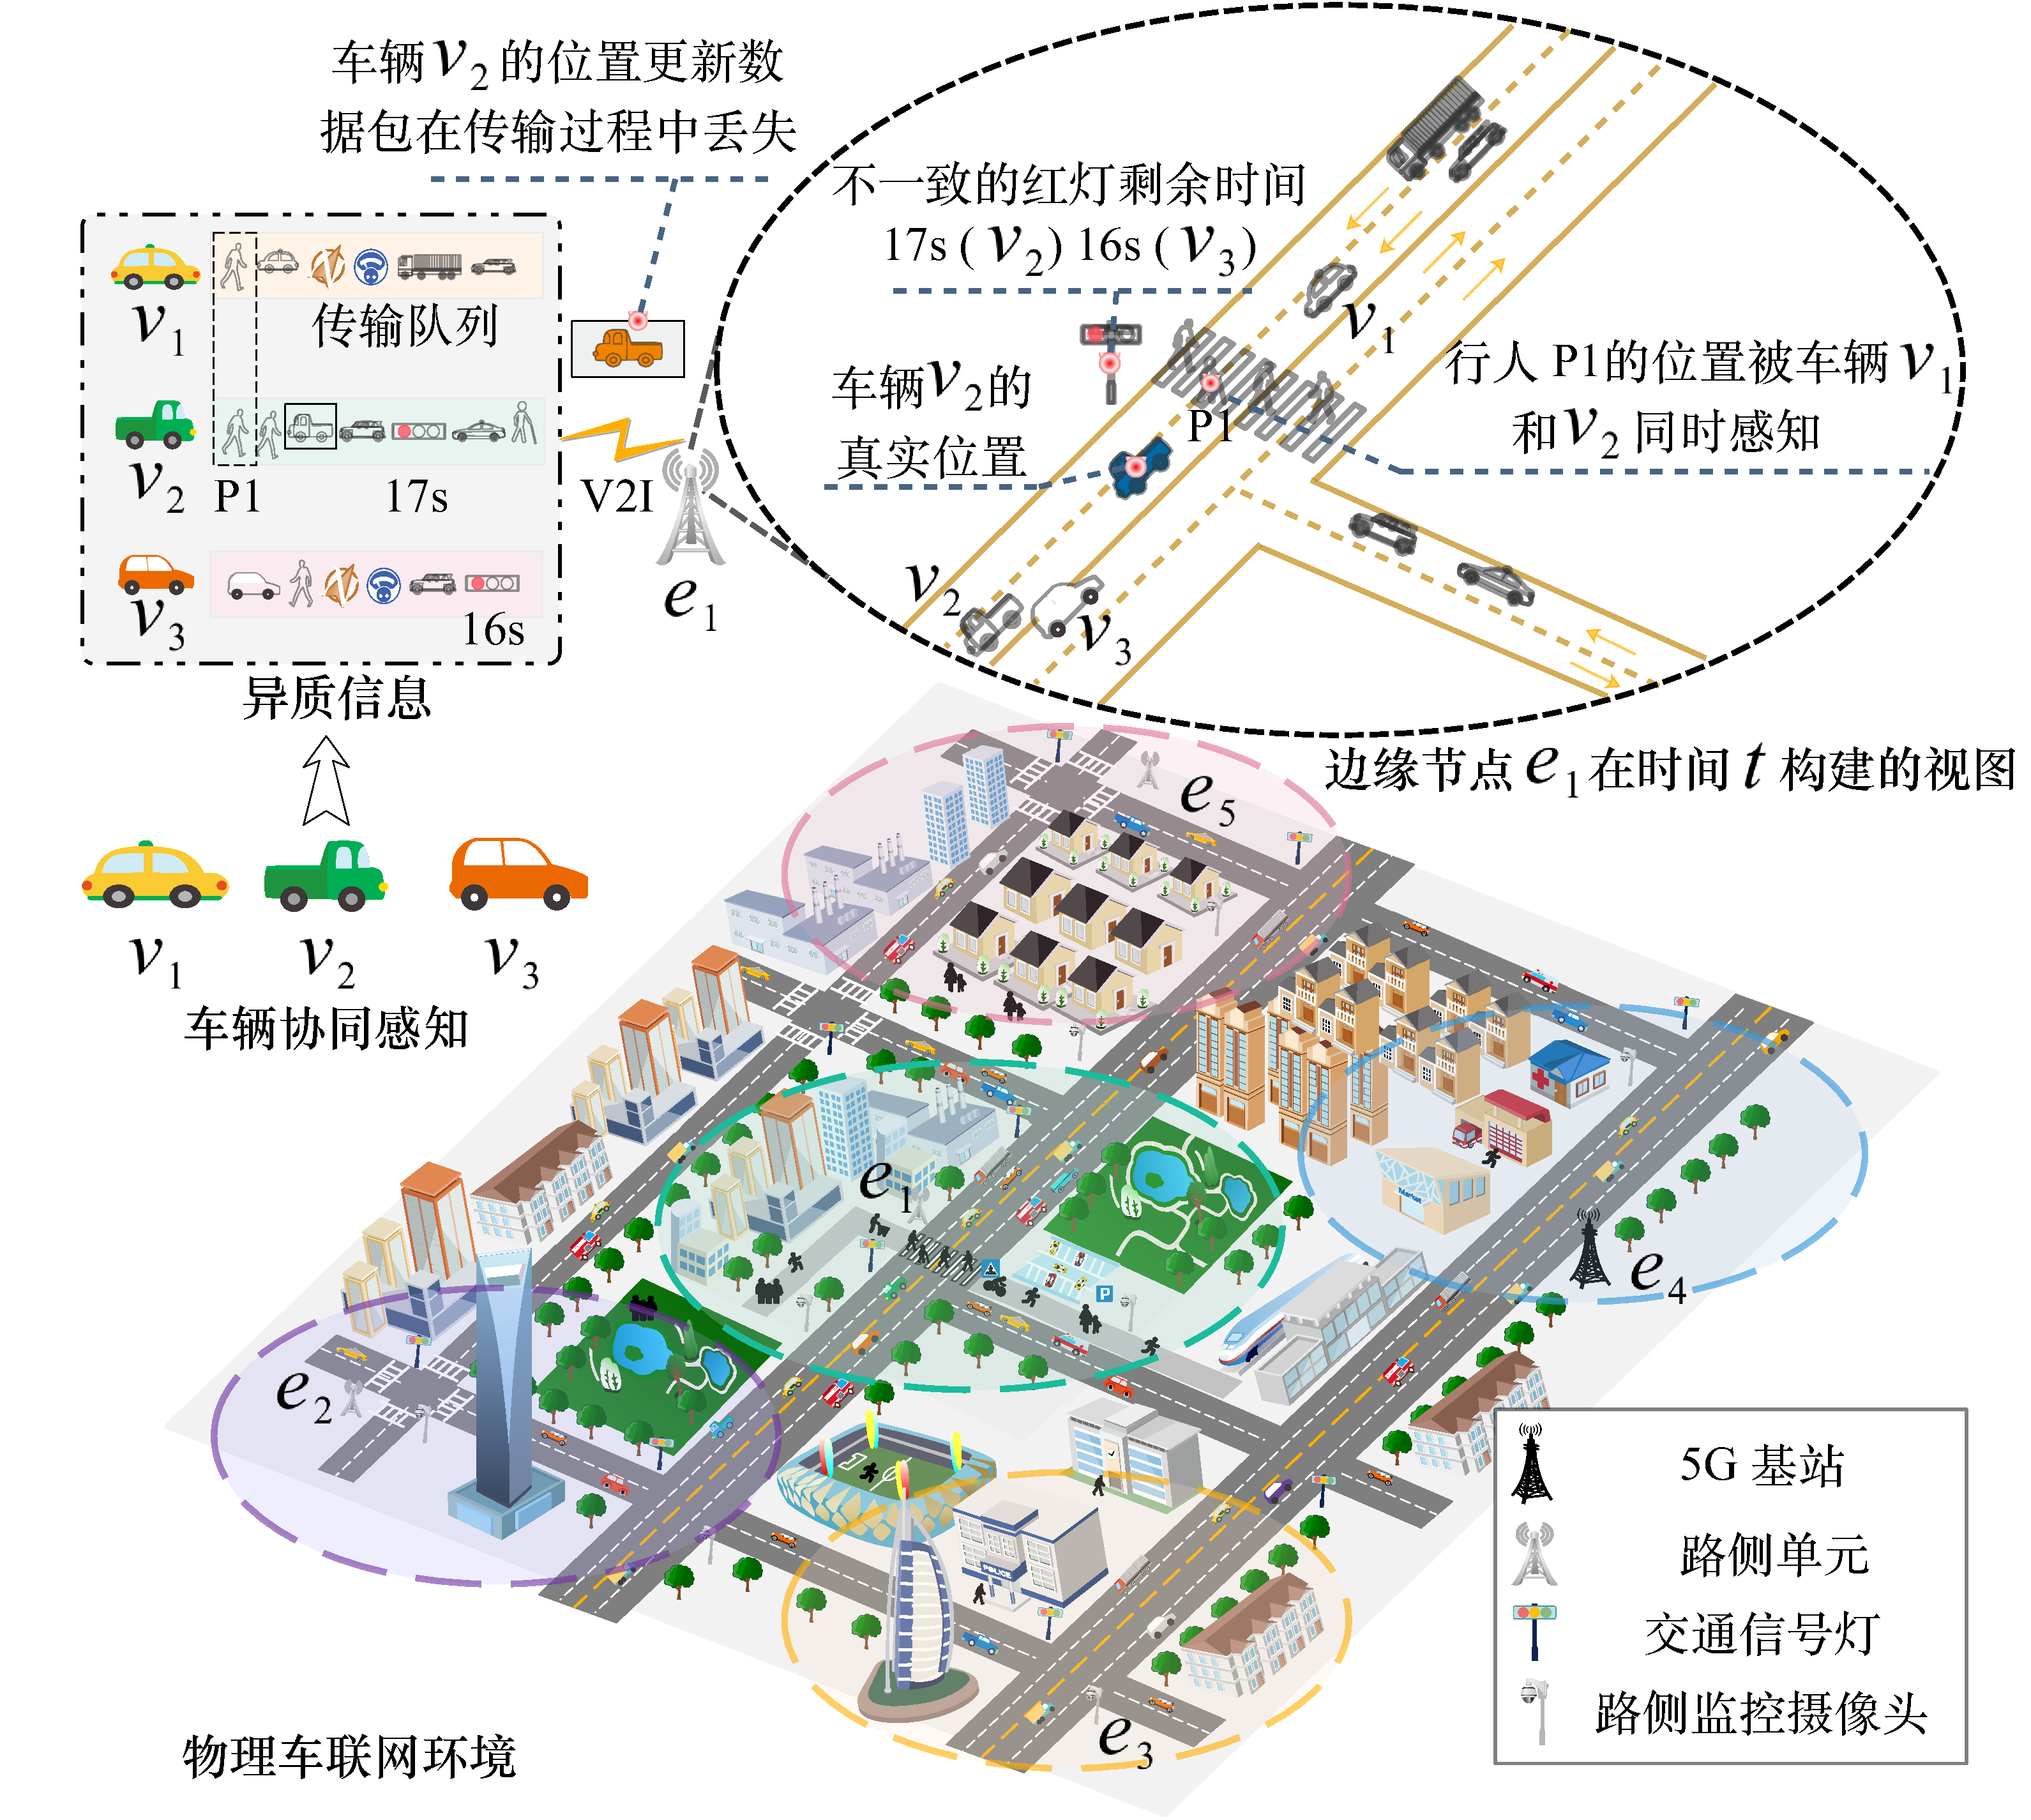
\includegraphics[width=0.47\textwidth]{fig/Fig2-2a-architerture.pdf}
\end{figure}
\end{textblock*}
\end{center}

\begin{center}
\begin{textblock*}{\textwidth}(0.5cm,2.1cm)
\begin{itemize}[itemsep=0.2\baselineskip]  \englishfont
	\item[\ding{111}] {\color{cqublue}{工作流程}}
	\begin{itemize}[itemsep=0.2\baselineskip] 
	\begin{small}
		\item[\ding{226}] \underline{感知}:感知频率、上传优先级
		\item[\ding{226}] \underline{上传}:V2I带宽
		\item[\ding{226}] \underline{视图构建}:信息融合,支撑 ITS 应用
	\end{small}
	\end{itemize}
	\item[\ding{111}]  {\color{cqublue}{速度建议应用为例}}
	\begin{itemize}[itemsep=0.2\baselineskip] 
	\begin{small}
		\item[\ding{226}] 信息不一致
			\begin{itemize}[itemsep=0.2\baselineskip]  \footnotesize
				\item[\ding{61}] 红灯剩余时间 {\color{cqublue}{17s}} (车辆$v_2$) {\color{cqublue}{16s}} (车辆$v_3$)
			\end{itemize}
		\item[\ding{226}] 重复感知
		\begin{itemize}[itemsep=0.2\baselineskip]  \footnotesize
			\item[\ding{61}] 同一物理要素的状态被多车感知
		\end{itemize}
		\item[\ding{226}] 物理环境与视图的差异
			\begin{itemize} [itemsep=0.2\baselineskip] \footnotesize
				\item[\ding{61}]数据包丢失 (车辆$v_2$的位置)
			\end{itemize}
		\item 
	\end{small} 
	\end{itemize}
\end{itemize}
\end{textblock*}
\end{center}
\end{frame}

\begin{frame}
\frametitle{\englishfont \underline{指标}:协同感知模型}
\newBackground
\begin{center}
\begin{textblock*}{\textwidth}(5.2cm,2.2cm)
\begin{figure}
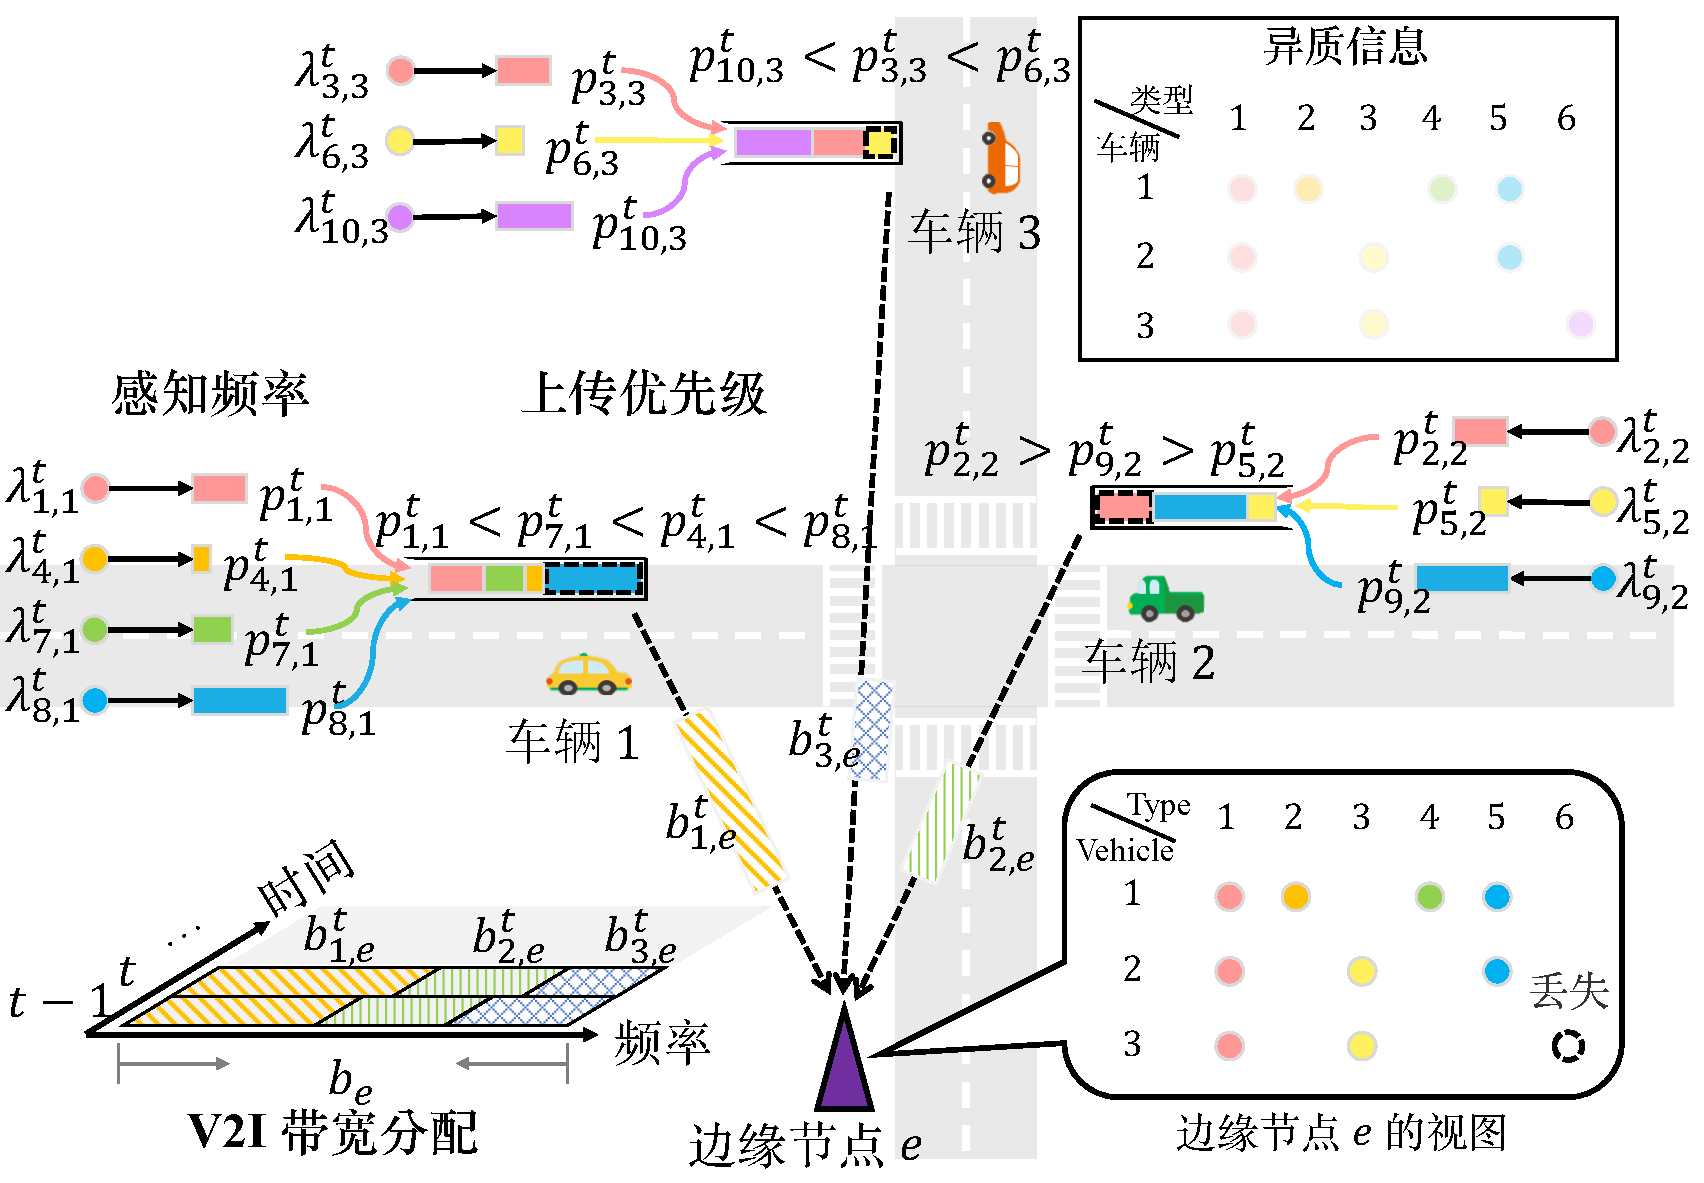
\includegraphics[width=0.55\textwidth]{fig/Fig2-3-cooperative-sensing.pdf}
\end{figure}
\end{textblock*}
\end{center}

% 添加动画效果

\begin{overlayarea}{\textwidth}{3cm}
\only<1-2>{
\begin{center}
\begin{textblock*}{1\textwidth}(-2cm,2.0cm)
\footnotesize
\begin{equation}
	\operatorname{\bar{q}}_{d, v}^t= \frac{1} {1 - \rho_{d, v}^{t}} 
        \left[ \alpha_{d, v}^t + \frac{ \lambda_{d, v}^{t} \beta_{d, v}^t + \sum\limits_{\forall d^* \in \mathbf{D}_{d, v}^t} \lambda_{d^*,s}^t \beta_{d^*, v}^t }{2\left(1-\rho_{d, v}^{t} - \lambda_{d, v}^{t}  \alpha_{d, v}^t\right)}\right] 
        - \alpha_{d, v}^t \notag
\end{equation}
\end{textblock*}
\end{center}
}

\only<2->{%
\begin{center}
\begin{textblock*}{1\textwidth}(-2cm,2.0cm)
\footnotesize
\begin{equation}
	\operatorname{\bar{q}}_{d, v}^t= \frac{1} {1 - \rho_{d, v}^{t}} 
        \left[ \alpha_{d, v}^t + \frac{ {\color{red}{ \lambda_{d, v}^{t} }}\beta_{d, v}^t + \sum\limits_{\forall d^* \in \mathbf{D}_{d, v}^t} \lambda_{d^*,s}^t \beta_{d^*, v}^t }{2\left(1-\rho_{d, v}^{t} - \lambda_{d, v}^{t}  \alpha_{d, v}^t\right)}\right] 
        - \alpha_{d, v}^t \notag
\end{equation}
\end{textblock*}
\end{center}
}

\only<3-4>{
\begin{center}
\begin{textblock*}{1\textwidth}(-3cm,4.9cm)
\footnotesize
\begin{equation}
\mathrm{w}_{d, v, e}^t=\frac{\left|d\right|}{b_{v, e}^{t} \log _{2}\left(1+\mathrm{SNR}_{v, e}^{t}\right)} \notag
\end{equation}
\end{textblock*}
\end{center}
}
\only<4->{
\begin{center}
\begin{textblock*}{1\textwidth}(-3cm,4.9cm)
\footnotesize
\begin{equation}
\mathrm{w}_{d, v, e}^t=\frac{\left|d\right|}{{\color{red}{b_{v, e}^{t}}} \log _{2}\left(1+\mathrm{SNR}_{v, e}^{t}\right)} \notag
\end{equation}
\end{textblock*}
\end{center}
}
\end{overlayarea}

\begin{center}
\begin{textblock*}{0.6\textwidth}(0.5cm,1.8cm)
\begin{itemize} \englishfont
	\item[\ding{111}]  {\color{cqublue}{排队时间}}
	\item 
	\item
	\item
	\item<2-> {\small{{\color{red}{ $\lambda_{d, v}^{t}$ }}:信息感知频率}}
	\item<3->[\ding{111}] {\color{cqublue}{传输时间}}
	\item
	\item 
	\item<4-> {\color{red}{$b_{v, e}^{t}$}}:V2I带宽
	\item<5->[\ding{111}] {\color{cqublue}{传输成功与否}}
		\begin{itemize}
		\begin{small}
			\item[\ding{226}] $\mathrm{SNR}_{\text {wall }}=\frac{\sigma^{2}-1}{\sigma}$
		\end{small}
	\end{itemize}
\end{itemize}
\end{textblock*}
\end{center}
\end{frame}

\begin{frame}{车载信息物理融合质量指标设计}
\frametitle{\englishfont \underline{指标}:Age of View}
\newBackground
\begin{overlayarea}{\textwidth}{3cm}
\only<1-1>{
\begin{center}
\begin{textblock*}{1\textwidth}(-3cm,1.8cm)
\begin{equation}
\Xi_{i}= \sum_{\forall v \in \mathbf{V}} \sum_{\forall d \in \mathbf{D}_{i, e} \cap \mathbf{D}_v^t } \xi_{d, v} \notag
\end{equation}
\end{textblock*}
\end{center}
}

\only<2-2>{
\begin{center}
\begin{textblock*}{1\textwidth}(-3cm,1.8cm)
\begin{equation}
\Xi_{i}= \sum_{\forall v \in \mathbf{V}} \sum_{\forall d \in \mathbf{D}_{i, e} \cap \mathbf{D}_v^t } {\color{red}{ \xi_{d, v}}} \notag
\end{equation}
\end{textblock*}
\end{center}
}

\only<3->{
\begin{center}
\begin{textblock*}{1\textwidth}(-3cm,1.8cm)
\begin{equation}
\Xi_{i}= \sum_{\forall v \in \mathbf{V}} \sum_{\forall d \in \mathbf{D}_{i, e} \cap \mathbf{D}_v^t }  \xi_{d, v} \notag
\end{equation}
\end{textblock*}
\end{center}
}

\only<2-2>{
\begin{center}
\begin{textblock*}{1\textwidth}(2cm,1.8cm)
\begin{equation}
{\color{red}{\xi_{d,v}}} = \operatorname{a}_{d, v}^t + \operatorname{q}_{d, v}^t + \operatorname{w}_{d, v, e}^t \notag
\end{equation}
\end{textblock*}
\end{center}
}
\only<3-3>{
\begin{center}
\begin{textblock*}{1\textwidth}(2cm,1.8cm)
\begin{equation}
\xi_{d,v} = {\color{red}{\operatorname{a}_{d, v}^t}} + \operatorname{q}_{d, v}^t + \operatorname{w}_{d, v, e}^t \notag
\end{equation}
\end{textblock*}
\end{center}
}

\only<3-3>{
\begin{center}
\begin{textblock*}{1\textwidth}(1.7cm,3.1cm)
\small
{\color{red}{$\operatorname{a}_{d, v}^t$}}:间隔到达时间
\end{textblock*}
\end{center}
}

\only<4-4>{
\begin{center}
\begin{textblock*}{1\textwidth}(2cm,1.8cm)
\begin{equation}
\xi_{d,v} = \operatorname{a}_{d, v}^t + {\color{red}{\operatorname{q}_{d, v}^t}} + \operatorname{w}_{d, v, e}^t \notag
\end{equation}
\end{textblock*}
\end{center}
}

\only<4-4>{
\begin{center}
\begin{textblock*}{1\textwidth}(1.7cm,3.1cm)
\small
{\color{red}{$\operatorname{q}_{d, v}^t$}}:排队时间
\end{textblock*}
\end{center}
}

\only<5-5>{
\begin{center}
\begin{textblock*}{1\textwidth}(2cm,1.8cm)
\begin{equation}
\xi_{d,v} = \operatorname{a}_{d, v}^t + \operatorname{q}_{d, v}^t + {\color{red}{\operatorname{w}_{d, v, e}^t}} \notag
\end{equation}
\end{textblock*}
\end{center}
}

\only<5-5>{
\begin{center}
\begin{textblock*}{1\textwidth}(1.7cm,3.1cm)
\small
{\color{red}{$\operatorname{w}_{d, v, e}^t$}}:传输时间
\end{textblock*}
\end{center}
}

\only<6->{
\begin{center}
\begin{textblock*}{1\textwidth}(2cm,1.8cm)
\begin{equation}
\xi_{d,v} = \operatorname{a}_{d, v}^t + \operatorname{q}_{d, v}^t + \operatorname{w}_{d, v, e}^t \notag
\end{equation}
\end{textblock*}
\end{center}
}

\only<1-5>{
\begin{center}
\begin{textblock*}{1\textwidth}(-3.6cm,3.6cm)
\begin{equation}
\Phi_{i} = {| \mathbf{D}_{i, e} |} \big/ {|D_{i} |} \notag
\end{equation}
\end{textblock*}
\end{center}
}

\only<6-6>{
\begin{center}
\begin{textblock*}{1\textwidth}(-3.6cm,3.6cm)
\begin{equation}
\Phi_{i} = {{\color{red}{| \mathbf{D}_{i, e} |}}} \big/ {|D_{i} |} \notag
\end{equation}
\end{textblock*}
\end{center}
}

\only<6-6>{
\begin{center}
\begin{textblock*}{1\textwidth}(1.5cm,4.2cm)
\small
{\color{red}{${| \mathbf{D}_{i, e} |}$}}:收到信息数量
\end{textblock*}
\end{center}
}

\only<7-7>{
\begin{center}
\begin{textblock*}{1\textwidth}(-3.6cm,3.6cm)
\begin{equation}
\Phi_{i} = {| \mathbf{D}_{i, e} |} \big/ {{\color{red}{|D_{i} |}}} \notag
\end{equation}
\end{textblock*}
\end{center}
}

\only<7-7>{
\begin{center}
\begin{textblock*}{1\textwidth}(1.5cm,4.2cm)
\small
{\color{red}{$|D_{i} |$}}:所需信息总量
\end{textblock*}
\end{center}
}

\only<8->{
\begin{center}
\begin{textblock*}{1\textwidth}(-3.6cm,3.6cm)
\begin{equation}
\Phi_{i} = {| \mathbf{D}_{i, e} |} \big/ {|D_{i} |} \notag
\end{equation}
\end{textblock*}
\end{center}
}

\only<1-7>{
\begin{center}
\begin{textblock*}{1\textwidth}(-1.7cm,4.8cm)
\begin{equation}
\Psi_{i}=\sum_{\forall v \in \mathbf{V}} \sum_{\forall d \in \mathbf{D}_{i, e} \cap \mathbf{D}_v^t} \left|\operatorname{q}_{d, v}^t + \operatorname{w}_{d, v, e}^t - \psi_{i} \right|^{2} \notag
\end{equation}
\end{textblock*}
\end{center}
}

\only<8-8>{
\begin{center}
\begin{textblock*}{1\textwidth}(-1.7cm,4.8cm)
\begin{equation}
\Psi_{i}=\sum_{\forall v \in \mathbf{V}} \sum_{\forall d \in \mathbf{D}_{i, e} \cap \mathbf{D}_v^t} \left| {\color{red}{\operatorname{q}_{d, v}^t + \operatorname{w}_{d, v, e}^t}} - \psi_{i} \right|^{2} \notag
\end{equation}
\end{textblock*}
\end{center}
}

\only<8-8>{
\begin{center}
\begin{textblock*}{1\textwidth}(5cm,5.4cm)
\small
{\color{red}{$\operatorname{q}_{d, v}^t + \operatorname{w}_{d, v, e}^t$}}:信息接收时间
\end{textblock*}
\end{center}
}

\only<9-9>{
\begin{center}
\begin{textblock*}{1\textwidth}(-1.7cm,4.8cm)
\begin{equation}
\Psi_{i}=\sum_{\forall v \in \mathbf{V}} \sum_{\forall d \in \mathbf{D}_{i, e} \cap \mathbf{D}_v^t} \left|\operatorname{q}_{d, v}^t + \operatorname{w}_{d, v, e}^t - {\color{red}{\psi_{i}}}\right|^{2} \notag
\end{equation}
\end{textblock*}
\end{center}
}

\only<9-9>{
\begin{center}
\begin{textblock*}{1\textwidth}(4cm,5.4cm)
\small
{\color{red}{$\psi_{i}$}}:平均接收时间
\end{textblock*}
\end{center}
}

\only<10->{
\begin{center}
\begin{textblock*}{1\textwidth}(-1.7cm,4.8cm)
\begin{equation}
\Psi_{i}=\sum_{\forall v \in \mathbf{V}} \sum_{\forall d \in \mathbf{D}_{i, e} \cap \mathbf{D}_v^t} \left|\operatorname{q}_{d, v}^t + \operatorname{w}_{d, v, e}^t - \psi_{i} \right|^{2} \notag
\end{equation}
\end{textblock*}
\end{center}
}
\end{overlayarea}


\begin{center}
\begin{textblock*}{1\textwidth}(1cm,1.8cm)
\begin{itemize} \englishfont
	\item[\ding{111}] {\color{cqublue}{时效性}}
	\item
	\item
	\item[\ding{111}]  {\color{cqublue}{完整性}}
	\item
	\item[\ding{111}]  {\color{cqublue}{一致性}}
	\item
	\item
	\item<10->[\ding{111}]  {\color{cqublue}{Age of View}}
	\begin{itemize}
	\begin{small}
		\item[\ding{226}] 归一化时效性、完整性和一致性的加权平均值
		\item[\ding{226}] $\operatorname{AoV}_{i} = w_1  \hat{\Xi}_{i} + w_2  \hat{\Phi}_{i}+  w_3 \hat{\Psi}_{i}$
	\end{small}
	\end{itemize}
\end{itemize}
\end{textblock*}
\end{center}
\end{frame}

\begin{frame}
\frametitle{\englishfont \underline{指标}:最大化VCPS质量问题}
\newBackground

\begin{overlayarea}{\textwidth}{3cm}
\only<1-1>{
\begin{center}
\begin{textblock*}{1\textwidth}(0.5cm,1.6cm)
\begin{align}
	\mathcal{P}2.1: &\max_{\boldsymbol{\Lambda}, \mathbf{P}, \mathbf{B}} \Upsilon \notag \\
	\text { s.t. }
    \mathcal{C}2.1: & \lambda_{d,v}^{t} \in \left [\lambda_{d,v}^{\min} , \lambda_{d,v}^{\max} \right ], \forall d \in \mathbf{D}_v^t , \forall v \in \mathbf{V}, \forall t \in \mathbf{T} \notag \\
     \mathcal{C}2.2: &{p}_{d^*, v}^t \neq {p}_{d, v}^t, \forall d^* \in \mathbf{D}_v^t \backslash \left\{ d\right \}, \forall d \in \mathbf{D}_v^t, \forall v \in \mathbf{V} \notag \\
    \mathcal{C}2.3: & b_{v, e}^t \in \left[ 0 , b_e \right ], \forall v \in \mathbf{V}_e^t, \forall e \in \mathbf{E}, \forall t \in \mathbf{T} \notag \\
    \mathcal{C}2.4: & \sum_{\forall d \subseteq \mathbf{D}_v^t} \lambda_{d,v}^{t}  \alpha_{d, v}^t < 1,\ \forall v \in \mathbf{V}, \forall t \in \mathbf{T}  \notag \\
    \mathcal{C}2.5: & {\sum_{\forall v \in \mathbf{V}_e^{t}}b_{v, e}^t} \leq b_e, \forall e \in \mathbf{E}, \forall t \in \mathbf{T} \notag
\end{align}	
\end{textblock*}
\end{center}
}

\only<2-2>{
\begin{center}
\begin{textblock*}{1\textwidth}(0.5cm,1.6cm)
\begin{align}
	\mathcal{P}2.1: &\max_{\boldsymbol{\Lambda}, \mathbf{P}, \mathbf{B}} {\color{red}{\Upsilon}} \notag \\
	\text { s.t. }
    \mathcal{C}2.1: & \lambda_{d,v}^{t} \in \left [\lambda_{d,v}^{\min} , \lambda_{d,v}^{\max} \right ], \forall d \in \mathbf{D}_v^t , \forall v \in \mathbf{V}, \forall t \in \mathbf{T} \notag \\
     \mathcal{C}2.2: &{p}_{d^*, v}^t \neq {p}_{d, v}^t, \forall d^* \in \mathbf{D}_v^t \backslash \left\{ d\right \}, \forall d \in \mathbf{D}_v^t, \forall v \in \mathbf{V} \notag \\
    \mathcal{C}2.3: & b_{v, e}^t \in \left[ 0 , b_e \right ], \forall v \in \mathbf{V}_e^t, \forall e \in \mathbf{E}, \forall t \in \mathbf{T} \notag \\
    \mathcal{C}2.4: & \sum_{\forall d \subseteq \mathbf{D}_v^t} \lambda_{d,v}^{t}  \alpha_{d, v}^t < 1,\ \forall v \in \mathbf{V}, \forall t \in \mathbf{T}  \notag \\
    \mathcal{C}2.5: & {\sum_{\forall v \in \mathbf{V}_e^{t}}b_{v, e}^t} \leq b_e, \forall e \in \mathbf{E}, \forall t \in \mathbf{T} \notag
\end{align}	
\end{textblock*}
\end{center}
}

\only<2-2>{
\begin{center}
\begin{textblock*}{1\textwidth}(0.5cm,7.1cm) \englishfont
{\color{red}{$\Upsilon$}}:VCPS质量 $\Upsilon=\frac{\sum_{\forall t \in \mathbf{T}} \sum_{\forall e \in \mathbf{E}} \sum_{\forall i \in \mathbf{I}_e^t} \left(1 - \operatorname{AoV}_{i}\right)}{\sum_{\forall t \in \mathbf{T}} \sum_{\forall e \in \mathbf{E}} |\mathbf{I}_e^t| }$
\end{textblock*}
\end{center}
}


\only<3-3>{
\begin{center}
\begin{textblock*}{1\textwidth}(0.5cm,1.6cm)
\begin{align}
	\mathcal{P}2.1: &\max_{{\color{red}{\boldsymbol{\Lambda}}}, \mathbf{P}, \mathbf{B}} \Upsilon \notag \\
	\text { s.t. }
    \mathcal{C}2.1: & \lambda_{d,v}^{t} \in \left [\lambda_{d,v}^{\min} , \lambda_{d,v}^{\max} \right ], \forall d \in \mathbf{D}_v^t , \forall v \in \mathbf{V}, \forall t \in \mathbf{T} \notag \\
     \mathcal{C}2.2: &{p}_{d^*, v}^t \neq {p}_{d, v}^t, \forall d^* \in \mathbf{D}_v^t \backslash \left\{ d\right \}, \forall d \in \mathbf{D}_v^t, \forall v \in \mathbf{V} \notag \\
    \mathcal{C}2.3: & b_{v, e}^t \in \left[ 0 , b_e \right ], \forall v \in \mathbf{V}_e^t, \forall e \in \mathbf{E}, \forall t \in \mathbf{T} \notag \\
    \mathcal{C}2.4: & \sum_{\forall d \subseteq \mathbf{D}_v^t} \lambda_{d,v}^{t}  \alpha_{d, v}^t < 1,\ \forall v \in \mathbf{V}, \forall t \in \mathbf{T}  \notag \\
    \mathcal{C}2.5: & {\sum_{\forall v \in \mathbf{V}_e^{t}}b_{v, e}^t} \leq b_e, \forall e \in \mathbf{E}, \forall t \in \mathbf{T} \notag
\end{align}	
\end{textblock*}
\end{center}
}

\only<3-3>{
\begin{center}
\begin{textblock*}{1\textwidth}(0.5cm,7.1cm) \englishfont
{\color{red}{$\boldsymbol{\Lambda}$}}:感知频率 $\boldsymbol{\Lambda} = \left\{ \lambda_{d, v}^{t} \vert \forall d \in \mathbf{D}_v^t  , \forall v \in \mathbf{V}, \forall t \in \mathbf{T} \right\}$
\end{textblock*}
\end{center}
}

\only<4-4>{
\begin{center}
\begin{textblock*}{1\textwidth}(0.5cm,1.6cm)
\begin{align}
	\mathcal{P}2.1: &\max_{\boldsymbol{\Lambda}, {\color{red}{\mathbf{P}}}, \mathbf{B}} \Upsilon \notag \\
	\text { s.t. }
    \mathcal{C}2.1: & \lambda_{d,v}^{t} \in \left [\lambda_{d,v}^{\min} , \lambda_{d,v}^{\max} \right ], \forall d \in \mathbf{D}_v^t , \forall v \in \mathbf{V}, \forall t \in \mathbf{T} \notag \\
     \mathcal{C}2.2: &{p}_{d^*, v}^t \neq {p}_{d, v}^t, \forall d^* \in \mathbf{D}_v^t \backslash \left\{ d\right \}, \forall d \in \mathbf{D}_v^t, \forall v \in \mathbf{V} \notag \\
    \mathcal{C}2.3: & b_{v, e}^t \in \left[ 0 , b_e \right ], \forall v \in \mathbf{V}_e^t, \forall e \in \mathbf{E}, \forall t \in \mathbf{T} \notag \\
    \mathcal{C}2.4: & \sum_{\forall d \subseteq \mathbf{D}_v^t} \lambda_{d,v}^{t}  \alpha_{d, v}^t < 1,\ \forall v \in \mathbf{V}, \forall t \in \mathbf{T}  \notag \\
    \mathcal{C}2.5: & {\sum_{\forall v \in \mathbf{V}_e^{t}}b_{v, e}^t} \leq b_e, \forall e \in \mathbf{E}, \forall t \in \mathbf{T} \notag
\end{align}	
\end{textblock*}
\end{center}
}

\only<4-4>{
\begin{center}
\begin{textblock*}{1\textwidth}(0.5cm,7.1cm) \englishfont
{\color{red}{$\mathbf{P}$}}:上传优先级 $\mathbf{P} = \left \{ p_{d, v}^{t} \vert \forall d \in \mathbf{D}_v^t, \forall v \in \mathbf{V}, \forall t \in \mathbf{T}\right \}$
\end{textblock*}
\end{center}
}

\only<5-5>{
\begin{center}
\begin{textblock*}{1\textwidth}(0.5cm,1.6cm)
\begin{align}
	\mathcal{P}2.1: &\max_{\boldsymbol{\Lambda}, \mathbf{P}, {\color{red}{\mathbf{B}}}} \Upsilon \notag \\
	\text { s.t. }
    \mathcal{C}2.1: & \lambda_{d,v}^{t} \in \left [\lambda_{d,v}^{\min} , \lambda_{d,v}^{\max} \right ], \forall d \in \mathbf{D}_v^t , \forall v \in \mathbf{V}, \forall t \in \mathbf{T} \notag \\
     \mathcal{C}2.2: &{p}_{d^*, v}^t \neq {p}_{d, v}^t, \forall d^* \in \mathbf{D}_v^t \backslash \left\{ d\right \}, \forall d \in \mathbf{D}_v^t, \forall v \in \mathbf{V} \notag \\
    \mathcal{C}2.3: & b_{v, e}^t \in \left[ 0 , b_e \right ], \forall v \in \mathbf{V}_e^t, \forall e \in \mathbf{E}, \forall t \in \mathbf{T} \notag \\
    \mathcal{C}2.4: & \sum_{\forall d \subseteq \mathbf{D}_v^t} \lambda_{d,v}^{t}  \alpha_{d, v}^t < 1,\ \forall v \in \mathbf{V}, \forall t \in \mathbf{T}  \notag \\
    \mathcal{C}2.5: & {\sum_{\forall v \in \mathbf{V}_e^{t}}b_{v, e}^t} \leq b_e, \forall e \in \mathbf{E}, \forall t \in \mathbf{T} \notag
\end{align}	
\end{textblock*}
\end{center}
}

\only<5-5>{
\begin{center}
\begin{textblock*}{1\textwidth}(0.5cm,7.1cm) \englishfont
{\color{red}{$\mathbf{B}$}}:V2I带宽分配 $\mathbf{B} = \left \{ b_{v, e}^t \vert \forall v \in \mathbf{V}_e^t, \forall e \in \mathbf{E}, \forall t \in \mathbf{T}\right \}$
\end{textblock*}
\end{center}
}

\only<6-6>{
\begin{center}
\begin{textblock*}{1\textwidth}(0.5cm,1.6cm)
\begin{align}
	\mathcal{P}2.1: &\max_{\boldsymbol{\Lambda}, \mathbf{P}, \mathbf{B}} \Upsilon \notag \\
	\text { s.t. }
    {\color{red}{\mathcal{C}2.1}}: & \lambda_{d,v}^{t} \in \left [\lambda_{d,v}^{\min} , \lambda_{d,v}^{\max} \right ], \forall d \in \mathbf{D}_v^t , \forall v \in \mathbf{V}, \forall t \in \mathbf{T} \notag \\
     \mathcal{C}2.2: &{p}_{d^*, v}^t \neq {p}_{d, v}^t, \forall d^* \in \mathbf{D}_v^t \backslash \left\{ d\right \}, \forall d \in \mathbf{D}_v^t, \forall v \in \mathbf{V} \notag \\
    \mathcal{C}2.3: & b_{v, e}^t \in \left[ 0 , b_e \right ], \forall v \in \mathbf{V}_e^t, \forall e \in \mathbf{E}, \forall t \in \mathbf{T} \notag \\
    \mathcal{C}2.4: & \sum_{\forall d \subseteq \mathbf{D}_v^t} \lambda_{d,v}^{t}  \alpha_{d, v}^t < 1,\ \forall v \in \mathbf{V}, \forall t \in \mathbf{T}  \notag \\
    \mathcal{C}2.5: & {\sum_{\forall v \in \mathbf{V}_e^{t}}b_{v, e}^t} \leq b_e, \forall e \in \mathbf{E}, \forall t \in \mathbf{T} \notag
\end{align}	
\end{textblock*}
\end{center}
}

\only<6-6>{
\begin{center}
\begin{textblock*}{1\textwidth}(0.5cm,7.1cm) \englishfont
{\color{red}{$\mathcal{C}2.1$}}:车辆$v$中的信息$d$在时间$t$的感知频率应满足其感知能力的要求
\end{textblock*}
\end{center}
}

\only<7-7>{
\begin{center}
\begin{textblock*}{1\textwidth}(0.5cm,1.6cm)
\begin{align}
	\mathcal{P}2.1: &\max_{\boldsymbol{\Lambda}, \mathbf{P}, \mathbf{B}} \Upsilon \notag \\
	\text { s.t. }
    \mathcal{C}2.1: & \lambda_{d,v}^{t} \in \left [\lambda_{d,v}^{\min} , \lambda_{d,v}^{\max} \right ], \forall d \in \mathbf{D}_v^t , \forall v \in \mathbf{V}, \forall t \in \mathbf{T} \notag \\
     {\color{red}{\mathcal{C}2.2}}: &{p}_{d^*, v}^t \neq {p}_{d, v}^t, \forall d^* \in \mathbf{D}_v^t \backslash \left\{ d\right \}, \forall d \in \mathbf{D}_v^t, \forall v \in \mathbf{V} \notag \\
    \mathcal{C}2.3: & b_{v, e}^t \in \left[ 0 , b_e \right ], \forall v \in \mathbf{V}_e^t, \forall e \in \mathbf{E}, \forall t \in \mathbf{T} \notag \\
    \mathcal{C}2.4: & \sum_{\forall d \subseteq \mathbf{D}_v^t} \lambda_{d,v}^{t}  \alpha_{d, v}^t < 1,\ \forall v \in \mathbf{V}, \forall t \in \mathbf{T}  \notag \\
    \mathcal{C}2.5: & {\sum_{\forall v \in \mathbf{V}_e^{t}}b_{v, e}^t} \leq b_e, \forall e \in \mathbf{E}, \forall t \in \mathbf{T} \notag
\end{align}	
\end{textblock*}
\end{center}
}

\only<7-7>{
\begin{center}
\begin{textblock*}{1\textwidth}(0.5cm,7.1cm) \englishfont
{\color{red}{$\mathcal{C}2.2$}}:保证时间$t$内车辆$v$中信息$d$的上传优先级
\end{textblock*}
\end{center}
}

\only<8-8>{
\begin{center}
\begin{textblock*}{1\textwidth}(0.5cm,1.6cm)
\begin{align}
	\mathcal{P}2.1: &\max_{\boldsymbol{\Lambda}, \mathbf{P}, \mathbf{B}} \Upsilon \notag \\
	\text { s.t. }
    \mathcal{C}2.1: & \lambda_{d,v}^{t} \in \left [\lambda_{d,v}^{\min} , \lambda_{d,v}^{\max} \right ], \forall d \in \mathbf{D}_v^t , \forall v \in \mathbf{V}, \forall t \in \mathbf{T} \notag \\
     \mathcal{C}2.2: &{p}_{d^*, v}^t \neq {p}_{d, v}^t, \forall d^* \in \mathbf{D}_v^t \backslash \left\{ d\right \}, \forall d \in \mathbf{D}_v^t, \forall v \in \mathbf{V} \notag \\
    {\color{red}{\mathcal{C}2.3}}: & b_{v, e}^t \in \left[ 0 , b_e \right ], \forall v \in \mathbf{V}_e^t, \forall e \in \mathbf{E}, \forall t \in \mathbf{T} \notag \\
    \mathcal{C}2.4: & \sum_{\forall d \subseteq \mathbf{D}_v^t} \lambda_{d,v}^{t}  \alpha_{d, v}^t < 1,\ \forall v \in \mathbf{V}, \forall t \in \mathbf{T}  \notag \\
    \mathcal{C}2.5: & {\sum_{\forall v \in \mathbf{V}_e^{t}}b_{v, e}^t} \leq b_e, \forall e \in \mathbf{E}, \forall t \in \mathbf{T} \notag
\end{align}	
\end{textblock*}
\end{center}
}

\only<8-8>{
\begin{center}
\begin{textblock*}{1\textwidth}(0.5cm,7.1cm) \englishfont
{\color{red}{$\mathcal{C}2.3$}}:边缘节点$e$在时间$t$为车辆$v$分配的V2I带宽不能超过其带宽容量$b_e$
\end{textblock*}
\end{center}
}

\only<9-9>{
\begin{center}
\begin{textblock*}{1\textwidth}(0.5cm,1.6cm)
\begin{align}
	\mathcal{P}2.1: &\max_{\boldsymbol{\Lambda}, \mathbf{P}, \mathbf{B}} \Upsilon \notag \\
	\text { s.t. }
    \mathcal{C}2.1: & \lambda_{d,v}^{t} \in \left [\lambda_{d,v}^{\min} , \lambda_{d,v}^{\max} \right ], \forall d \in \mathbf{D}_v^t , \forall v \in \mathbf{V}, \forall t \in \mathbf{T} \notag \\
     \mathcal{C}2.2: &{p}_{d^*, v}^t \neq {p}_{d, v}^t, \forall d^* \in \mathbf{D}_v^t \backslash \left\{ d\right \}, \forall d \in \mathbf{D}_v^t, \forall v \in \mathbf{V} \notag \\
    \mathcal{C}2.3: & b_{v, e}^t \in \left[ 0 , b_e \right ], \forall v \in \mathbf{V}_e^t, \forall e \in \mathbf{E}, \forall t \in \mathbf{T} \notag \\
    {\color{red}{\mathcal{C}2.4}}: & \sum_{\forall d \subseteq \mathbf{D}_v^t} \lambda_{d,v}^{t}  \alpha_{d, v}^t < 1,\ \forall v \in \mathbf{V}, \forall t \in \mathbf{T}  \notag \\
    \mathcal{C}2.5: & {\sum_{\forall v \in \mathbf{V}_e^{t}}b_{v, e}^t} \leq b_e, \forall e \in \mathbf{E}, \forall t \in \mathbf{T} \notag
\end{align}	
\end{textblock*}
\end{center}
}

\only<9-9>{
\begin{center}
\begin{textblock*}{1\textwidth}(0.5cm,7.1cm) \englishfont
{\color{red}{$\mathcal{C}2.4$}}:保证在调度周期$\mathbf{T}$内队列稳定状态
\end{textblock*}
\end{center}
}

\only<10-10>{
\begin{center}
\begin{textblock*}{1\textwidth}(0.5cm,1.6cm)
\begin{align}
	\mathcal{P}2.1: &\max_{\boldsymbol{\Lambda}, \mathbf{P}, \mathbf{B}} \Upsilon \notag \\
	\text { s.t. }
    \mathcal{C}2.1: & \lambda_{d,v}^{t} \in \left [\lambda_{d,v}^{\min} , \lambda_{d,v}^{\max} \right ], \forall d \in \mathbf{D}_v^t , \forall v \in \mathbf{V}, \forall t \in \mathbf{T} \notag \\
     \mathcal{C}2.2: &{p}_{d^*, v}^t \neq {p}_{d, v}^t, \forall d^* \in \mathbf{D}_v^t \backslash \left\{ d\right \}, \forall d \in \mathbf{D}_v^t, \forall v \in \mathbf{V} \notag \\
    \mathcal{C}2.3: & b_{v, e}^t \in \left[ 0 , b_e \right ], \forall v \in \mathbf{V}_e^t, \forall e \in \mathbf{E}, \forall t \in \mathbf{T} \notag \\
    \mathcal{C}2.4: & \sum_{\forall d \subseteq \mathbf{D}_v^t} \lambda_{d,v}^{t}  \alpha_{d, v}^t < 1,\ \forall v \in \mathbf{V}, \forall t \in \mathbf{T}  \notag \\
    {\color{red}{\mathcal{C}2.5}}: & {\sum_{\forall v \in \mathbf{V}_e^{t}}b_{v, e}^t} \leq b_e, \forall e \in \mathbf{E}, \forall t \in \mathbf{T} \notag
\end{align}	
\end{textblock*}
\end{center}
}

\only<10-10>{
\begin{center}
\begin{textblock*}{1\textwidth}(0.5cm,7.1cm) \englishfont
{\color{red}{$\mathcal{C}2.5$}}:边缘节点$e$分配的V2I带宽之和不能超过其容量$b_e$
\end{textblock*}
\end{center}
}

\end{overlayarea}

\end{frame}

\begin{frame}
\frametitle{\englishfont \underline{算法}:流程}
\newBackground

\begin{center}
\begin{textblock*}{\textwidth}(4.8cm,2.4cm)
\begin{figure}
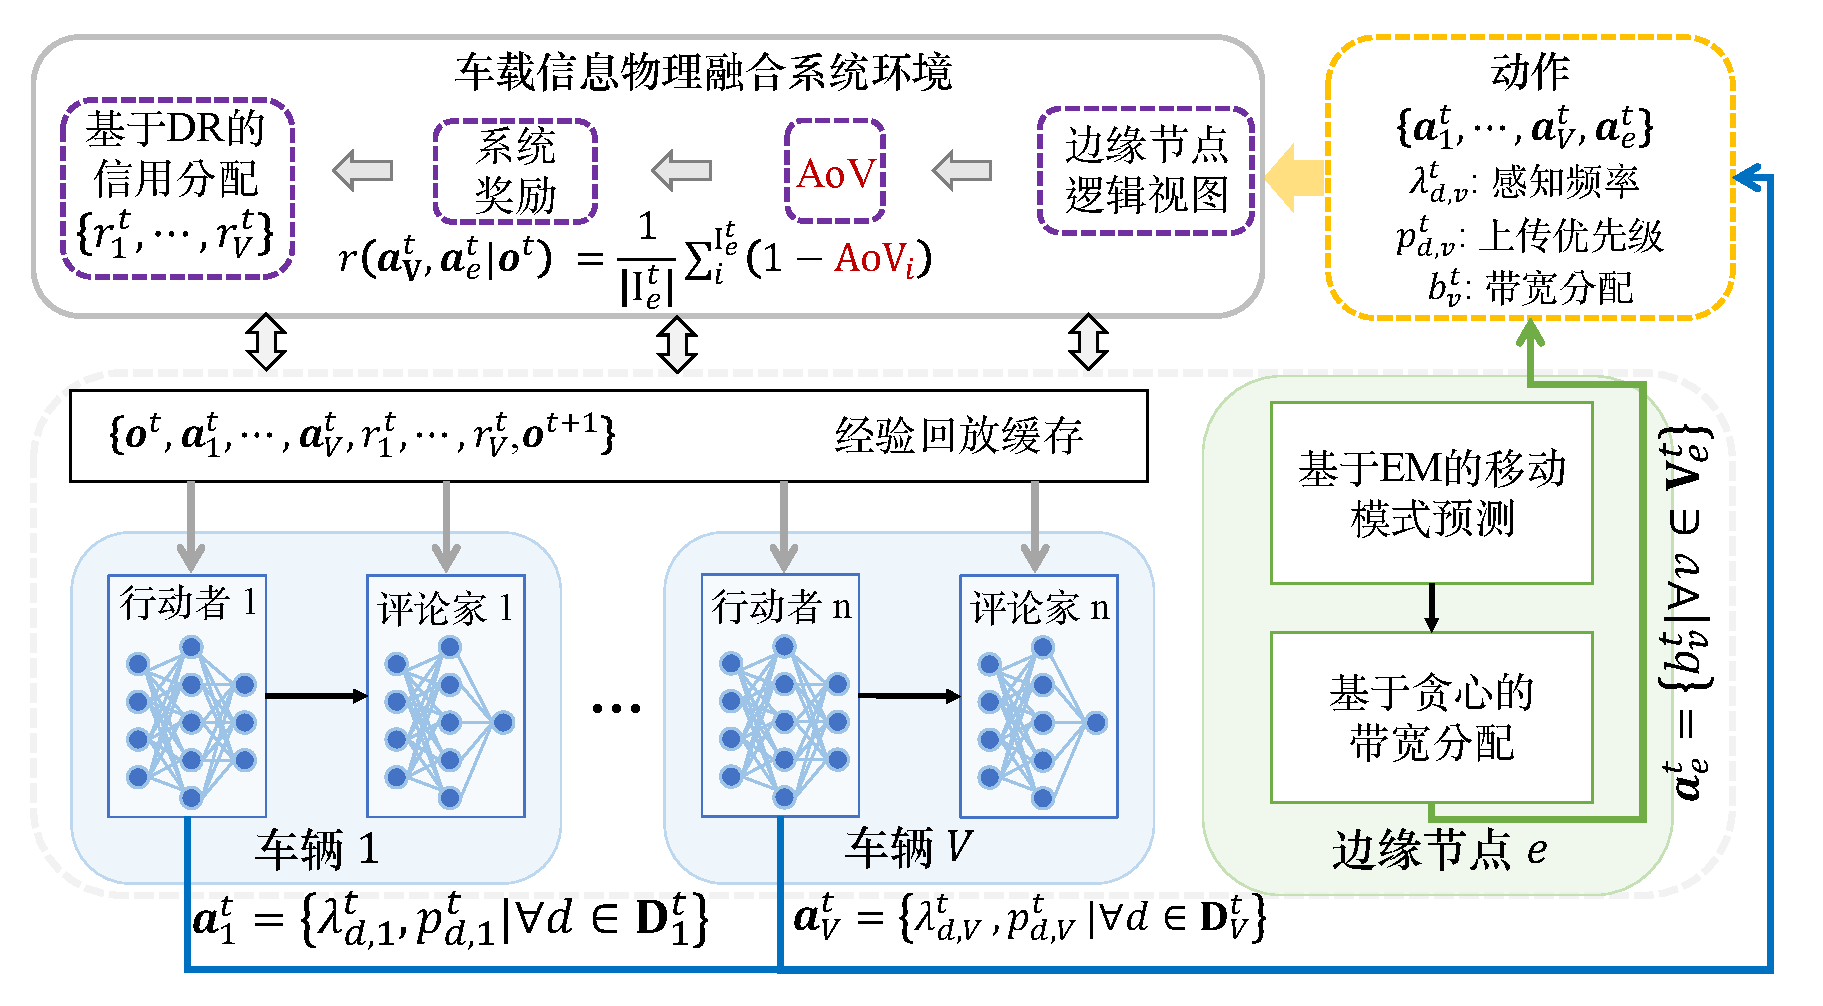
\includegraphics[width=0.6\textwidth]{fig/Fig2-4-solution-model.pdf}
\end{figure}
\end{textblock*}
\end{center}

\begin{center}
\begin{textblock*}{0.8\textwidth}(0cm,1.9cm)
\begin{itemize}[itemsep=0.2\baselineskip] \englishfont
	\item[\ding{111}] {\color{cqublue}{初始化}}
	\begin{itemize}[itemsep=0.2\baselineskip]
	\begin{small}
		\item[\ding{226}] 车辆行动者/评论家网络参数
		\item[\ding{226}] 经验回放缓存
		\end{small}
	\end{itemize}
	\item[\ding{111}]  {\color{cqublue}{回放经验存储}}
	\begin{itemize}[itemsep=0.2\baselineskip]
	\begin{small}
		\item[\ding{226}] 车辆决策{\small{$\boldsymbol{a}_{v}^{t}=\boldsymbol{\mu}_{\boldsymbol{v}}\left(\boldsymbol{o}_{v}^{t} \mid \theta_{v}^{\mu}\right)+\mathcal{N}_{t}$}}
		\item[\ding{226}] 边缘节点基于VBA机制分配带宽
		\item[\ding{226}] 存储与环境交互结果
	\end{small}
	\end{itemize}
	\item[\ding{111}]  {\color{cqublue}{训练}}
	\begin{itemize}[itemsep=0.2\baselineskip]
	\begin{small}
		\item[\ding{226}] 评论家网络损失函数\\{\small{$\mathcal{L}\left(\theta_{v}^{Q}\right)=\frac{1}{M} \Sigma_{m}\left(\eta_{m}-Q_{v}\left(\boldsymbol{o}_{v}^{m}, \boldsymbol{a}_{\mathbf{V}}^{m} \mid \theta_{v}^{Q}\right)\right)^{2}$}}
		\item[\ding{226}] 行动者网络策略梯度\\{\small{$\nabla_{\theta_{v}^{\mu}} \mathcal{J} \approx \frac{1}{M} \sum_{m} \nabla_{\boldsymbol{a}_{\mathbf{V}}^{m}} Q_{v}\left(\boldsymbol{o}_{v}^{m}, \boldsymbol{a}_{\mathbf{V}}^{m} \mid \theta_{v}^{Q}\right) \nabla_{\theta_{v}^{\mu}} \mu_{v}\left(\boldsymbol{o}_{v}^{m+1} \mid \theta_{v}^{\mu}\right)$}}
	\end{small}
	\end{itemize}
\end{itemize}
\end{textblock*}
\end{center}
\end{frame}

\begin{frame}
\frametitle{\englishfont \underline{算法}:MADR模型}
\newBackground
\begin{center}
\begin{textblock*}{\textwidth}(4.8cm,2.4cm)

\begin{figure}
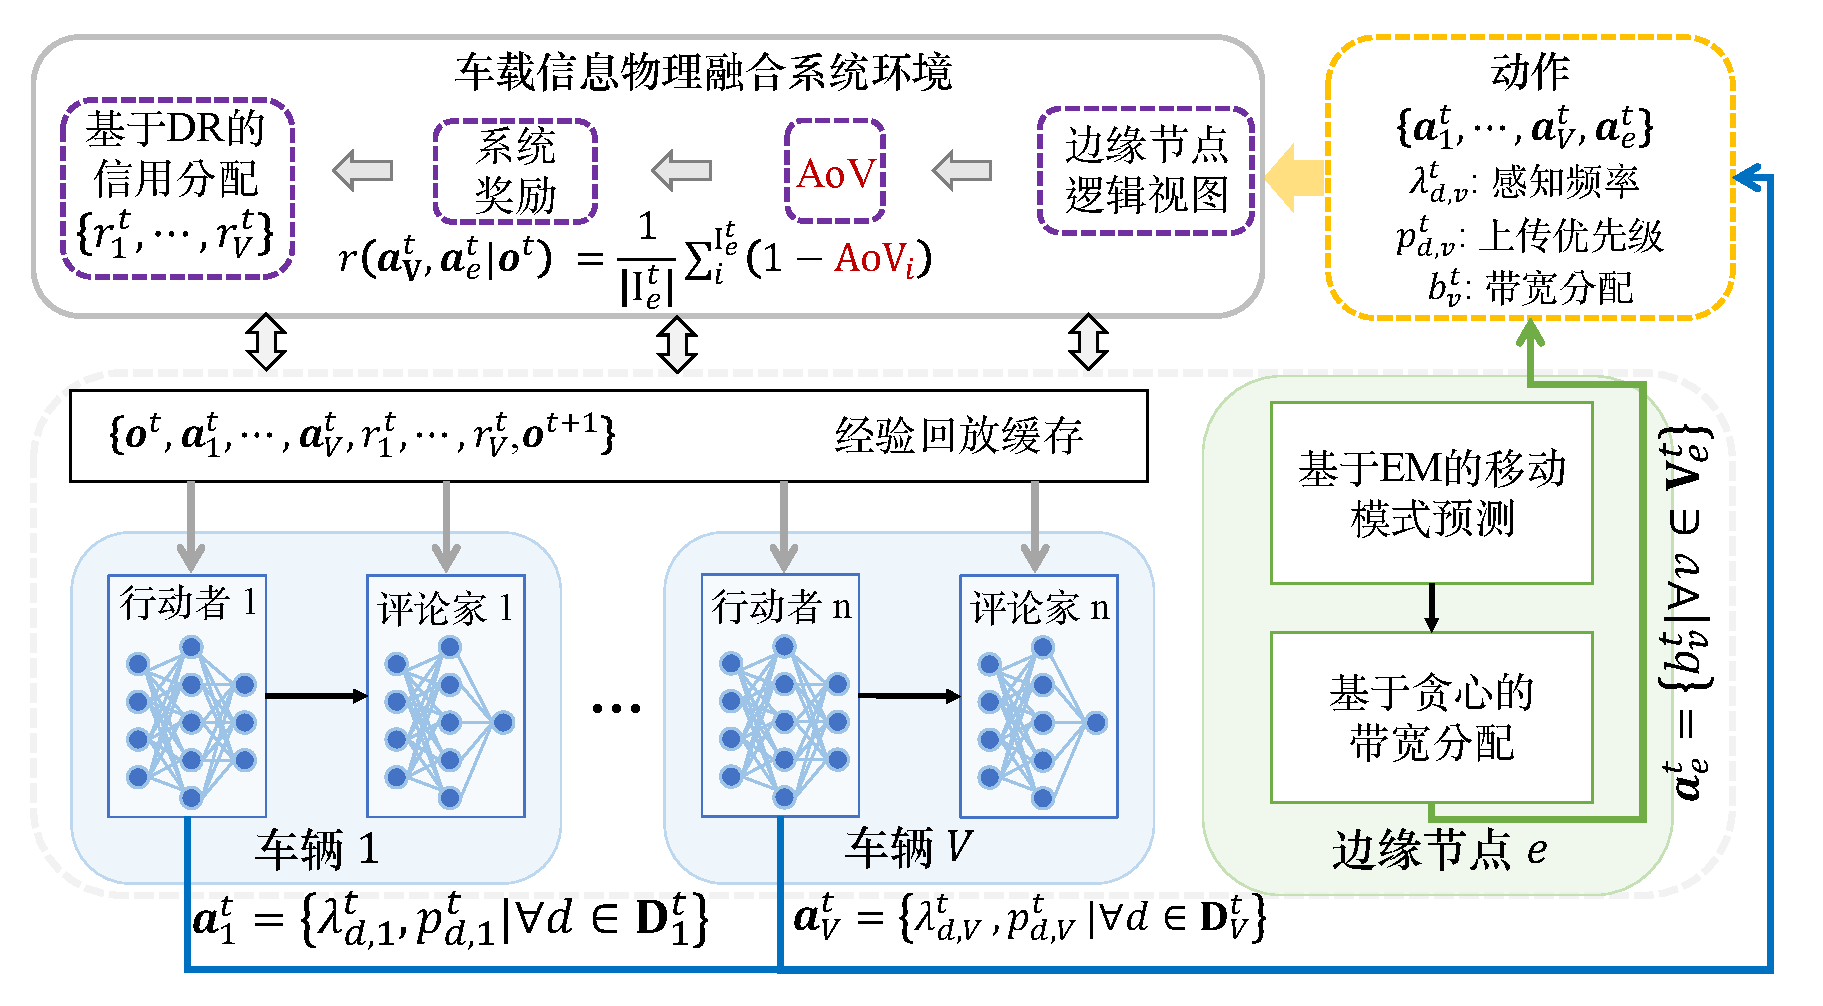
\includegraphics[width=0.6\textwidth]{fig/Fig2-4-solution-model.pdf}
\end{figure}
\end{textblock*}
\end{center}

\begin{center}
\begin{textblock*}{0.56\textwidth}(0.5cm,2cm)
\begin{itemize}[itemsep=0.2\baselineskip] \englishfont
	\item[\ding{111}] {\color{cqublue}{系统状态}}
	\begin{itemize}[itemsep=0.2\baselineskip]
	\begin{small}
		\item[\ding{226}] 车辆观测{\small{$\boldsymbol{o}_{v}^{t}=\left\{\mathbf{D}_{v}^{t}, \mathbf{D}_{e}^{t}, \mathbf{I}_e^t\right\}$}}
		\item[\ding{226}] {\small{$\boldsymbol{o}^{t}=\left\{\mathbf{D}_{1}^{t}, \ldots, \mathbf{D}_{v}^{t}, \ldots, \mathbf{D}_{V}^{t}, \mathbf{D}_{e}^{t}, \mathbf{I}_{e}^{t}\right\}$}}
	\end{small}
	\end{itemize}
	\item[\ding{111}]  {\color{cqublue}{动作空间}}
	\begin{itemize}[itemsep=0.2\baselineskip]
	\begin{small}
		\item[\ding{226}] {\small{$\boldsymbol{a}_{v}^{t}=\{ \lambda_{d, v}^{t}, p_{d, v}^{t} \mid \forall d \in \mathbf{D}_{v}^t\}$}}
		\item[\ding{226}] 车辆动作集合{\small{$\boldsymbol{a}_{\mathbf{V}}^{t} = \left\{\boldsymbol{a}_{v}^{t}\mid \forall v \in \mathbf{V}\right\}$}}
	\end{small}
	\end{itemize}
	\item[\ding{111}]  {\color{cqublue}{系统奖励}}
	\begin{itemize}[itemsep=0.2\baselineskip]
	\begin{small}
		\item[\ding{226}] {\small{$r\left(\boldsymbol{a}_{\mathbf{V}}^{t},\boldsymbol{a}_{e}^{t} \mid \boldsymbol{o}^{t}\right)=\frac{1}{\left|\mathbf{I}_e^t\right|} \sum_{\forall i \in \mathbf{I}_e^t}\left(1 -\operatorname{AoV}_{i} \right)$}}
		\item[\ding{226}] 车辆奖励:差分奖励分配机制\\{\small{$r_{v}^{t}=r\left(\boldsymbol{a}_{\mathbf{V}}^{t},\boldsymbol{a}_{e}^{t} \mid \boldsymbol{o}^{t}\right)-r\left(\boldsymbol{a}_{\mathbf{V}-v}^{t},\boldsymbol{a}_{e}^{t} \mid \boldsymbol{o}^{t}\right)$}}
	\end{small}
	\end{itemize}
\end{itemize}
\end{textblock*}
\end{center}
\end{frame}

\begin{frame}
\frametitle{\englishfont \underline{算法}:V2I 带宽分配机制 (VBA)}
\newBackground
\begin{center}
\begin{textblock*}{\textwidth}(4.8cm,2.4cm)
\begin{figure}
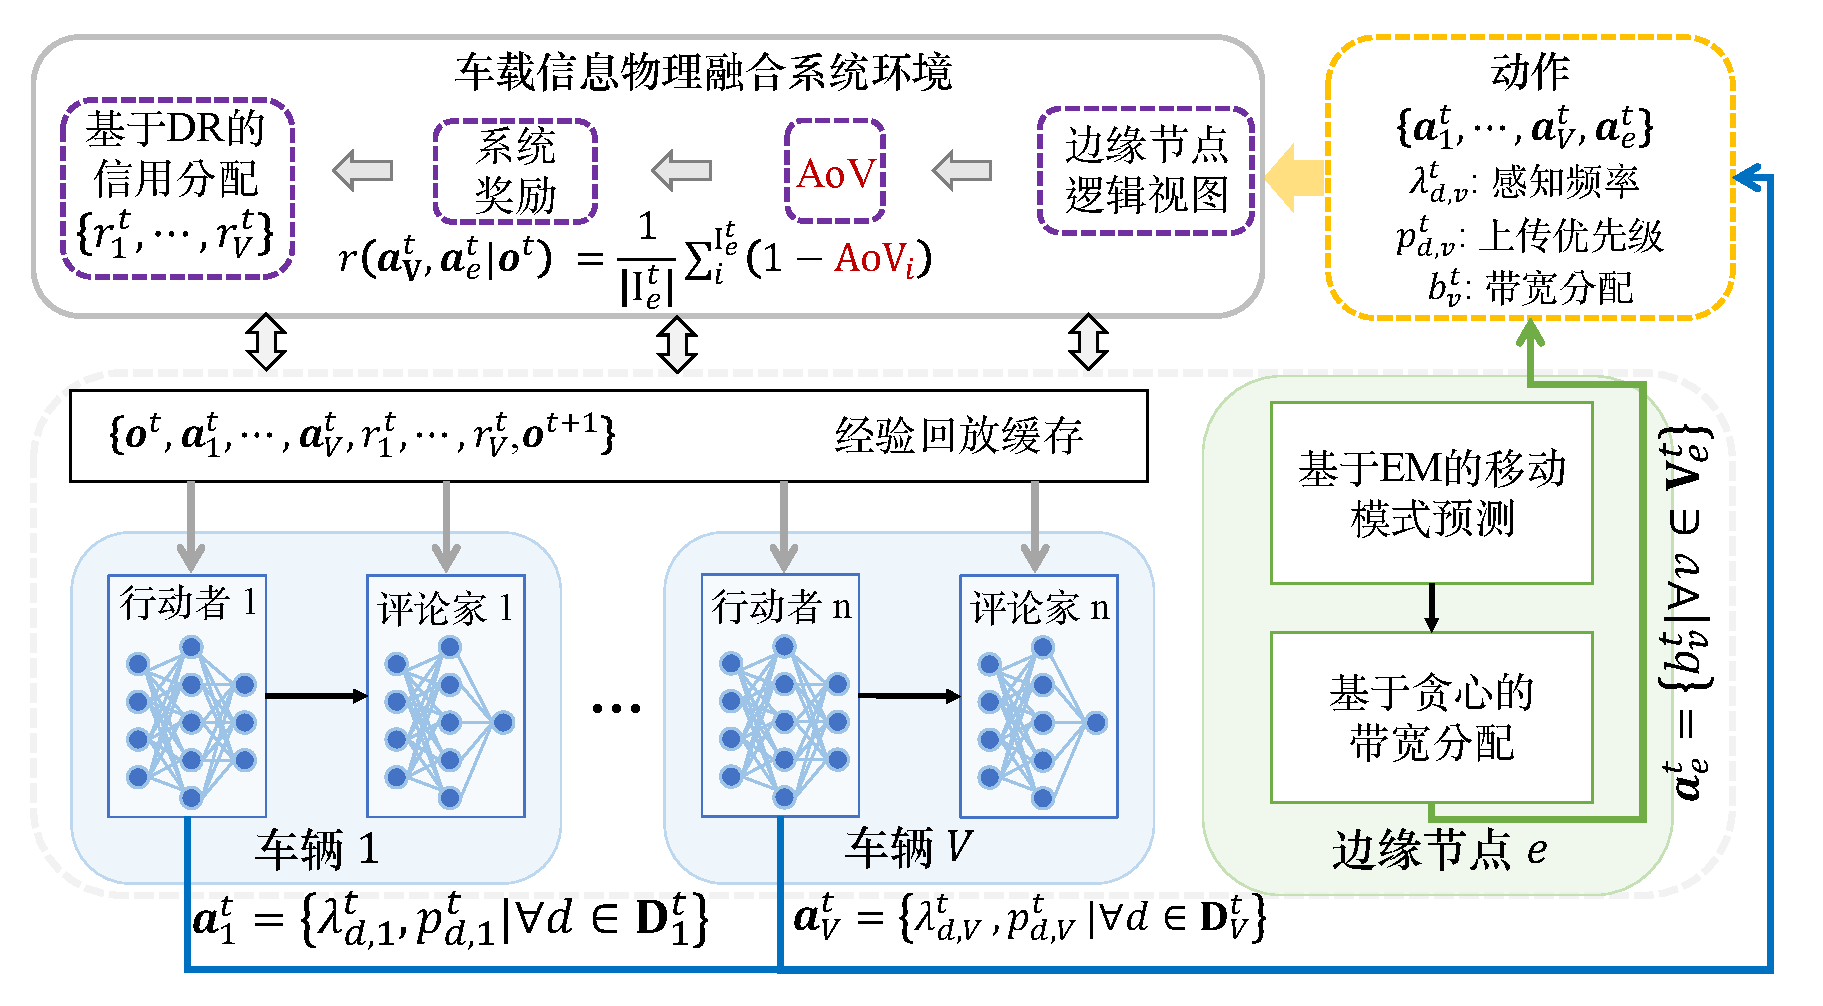
\includegraphics[width=0.6\textwidth]{fig/Fig2-4-solution-model.pdf}
\end{figure}
\end{textblock*}
\end{center}

\begin{center}
\begin{textblock*}{0.56\textwidth}(0.5cm,1.8cm)
\begin{itemize} \englishfont 
	\item[\ding{111}] {\color{cqublue}{距离估计}}
	\begin{itemize}[itemsep=0.2\baselineskip]
	\begin{small}
		\item[\ding{226}] 期望最大化 (EM)预测轨迹\\{\small{$\operatorname{Traj}_{v}^{t} = \{ \hat{l}_{v}^{t+1}, \dots, \hat{l}_{v}^{t+h}, \dots, \hat{l}_{v}^{t+H}\}$}}
		\item[\ding{226}] 平均距离{\small{$\operatorname{\bar{dis}}_{v, e}^{t} = \frac{1}{H} {\sum_{\forall h \in [1, H]} \widehat{\operatorname{dis}}_{v, e}^{t+h}}$}}
	\end{small}
	\end{itemize}
	\item[\ding{111}]  {\color{cqublue}{感知信息}}
	\begin{itemize}[itemsep=0.2\baselineskip]
	\begin{small}
		\item[\ding{226}] 视图$i$需要{\small{$\mathbf{D}_{v, i}^{t} = \left\{ d \mid  d \in \mathbf{D}_{v}^t \cap  \mathbf{D}_i \right\}$}}
		\item[\ding{226}] 视图需要{\small{$\mathbf{D}_{v, {\mathbf{I}_e^t}}^{t} = \{ d \mid  d \in \bigcup_{\forall v \in V_e^t} \mathbf{D}_{v, i}^{t}\}$}}
	\end{small}
	\end{itemize}
	\item[\ding{111}]  {\color{cqublue}{带宽分配}}
	\begin{itemize}[itemsep=0.2\baselineskip]
	\begin{small}
		\item[\ding{226}] {\small{$b_{v, e}^{t} =\frac{b_{e}} {\omega+\operatorname{rank}_{v}}$}}
		\item[\ding{226}] 按$| \mathbf{D}_{v, {\mathbf{I}_e^t}}^{t}|$的序列降序
		\item[\ding{226}] 按$\operatorname{\bar{dis}}_{v, e}^{t}$的序列升序
	\end{small}
	\end{itemize}
\end{itemize}
\end{textblock*}
\end{center}
\end{frame}


\begin{frame}
\frametitle{\englishfont \underline{实验}:数据与基本设置}
\newBackground

\begin{center}
	\begin{textblock*}{\textwidth}(-2.4cm,2.3cm)
	\begin{table}[h] \englishfont
\resizebox{0.45\textwidth}{!}{%
\begin{tabular}{cc}
\toprule 
\textbf{参数} & \textbf{值}         \\ \midrule
信息数据大小      & {[}100 B, 1 MB{]}  \\
传输功率        & 1 mW               \\
通信噪声        & -90 dBm            \\
带宽          & 3 MHz              \\
行动者         & 4 层全连接 (隐藏层 64-32)  \\
评论家         & 4 层全连接 (隐藏层 128-64) \\
学习率         & 0.001              \\
折扣因子        & 0.996              \\
经验回放缓存大小    & 100000             \\
批大小         & 512                \\ \bottomrule
\end{tabular}%
}
\end{table}
\end{textblock*}
\end{center}

\begin{center}
\begin{textblock*}{\textwidth}(0cm,1.8cm)
\begin{itemize} \englishfont \small
	\item[\ding{111}] {\color{cqublue}{实验与模型参数}}
\end{itemize}
\end{textblock*}
\end{center}

\begin{center}
\begin{textblock*}{\textwidth}(5cm,1.8cm)
	\begin{figure}
	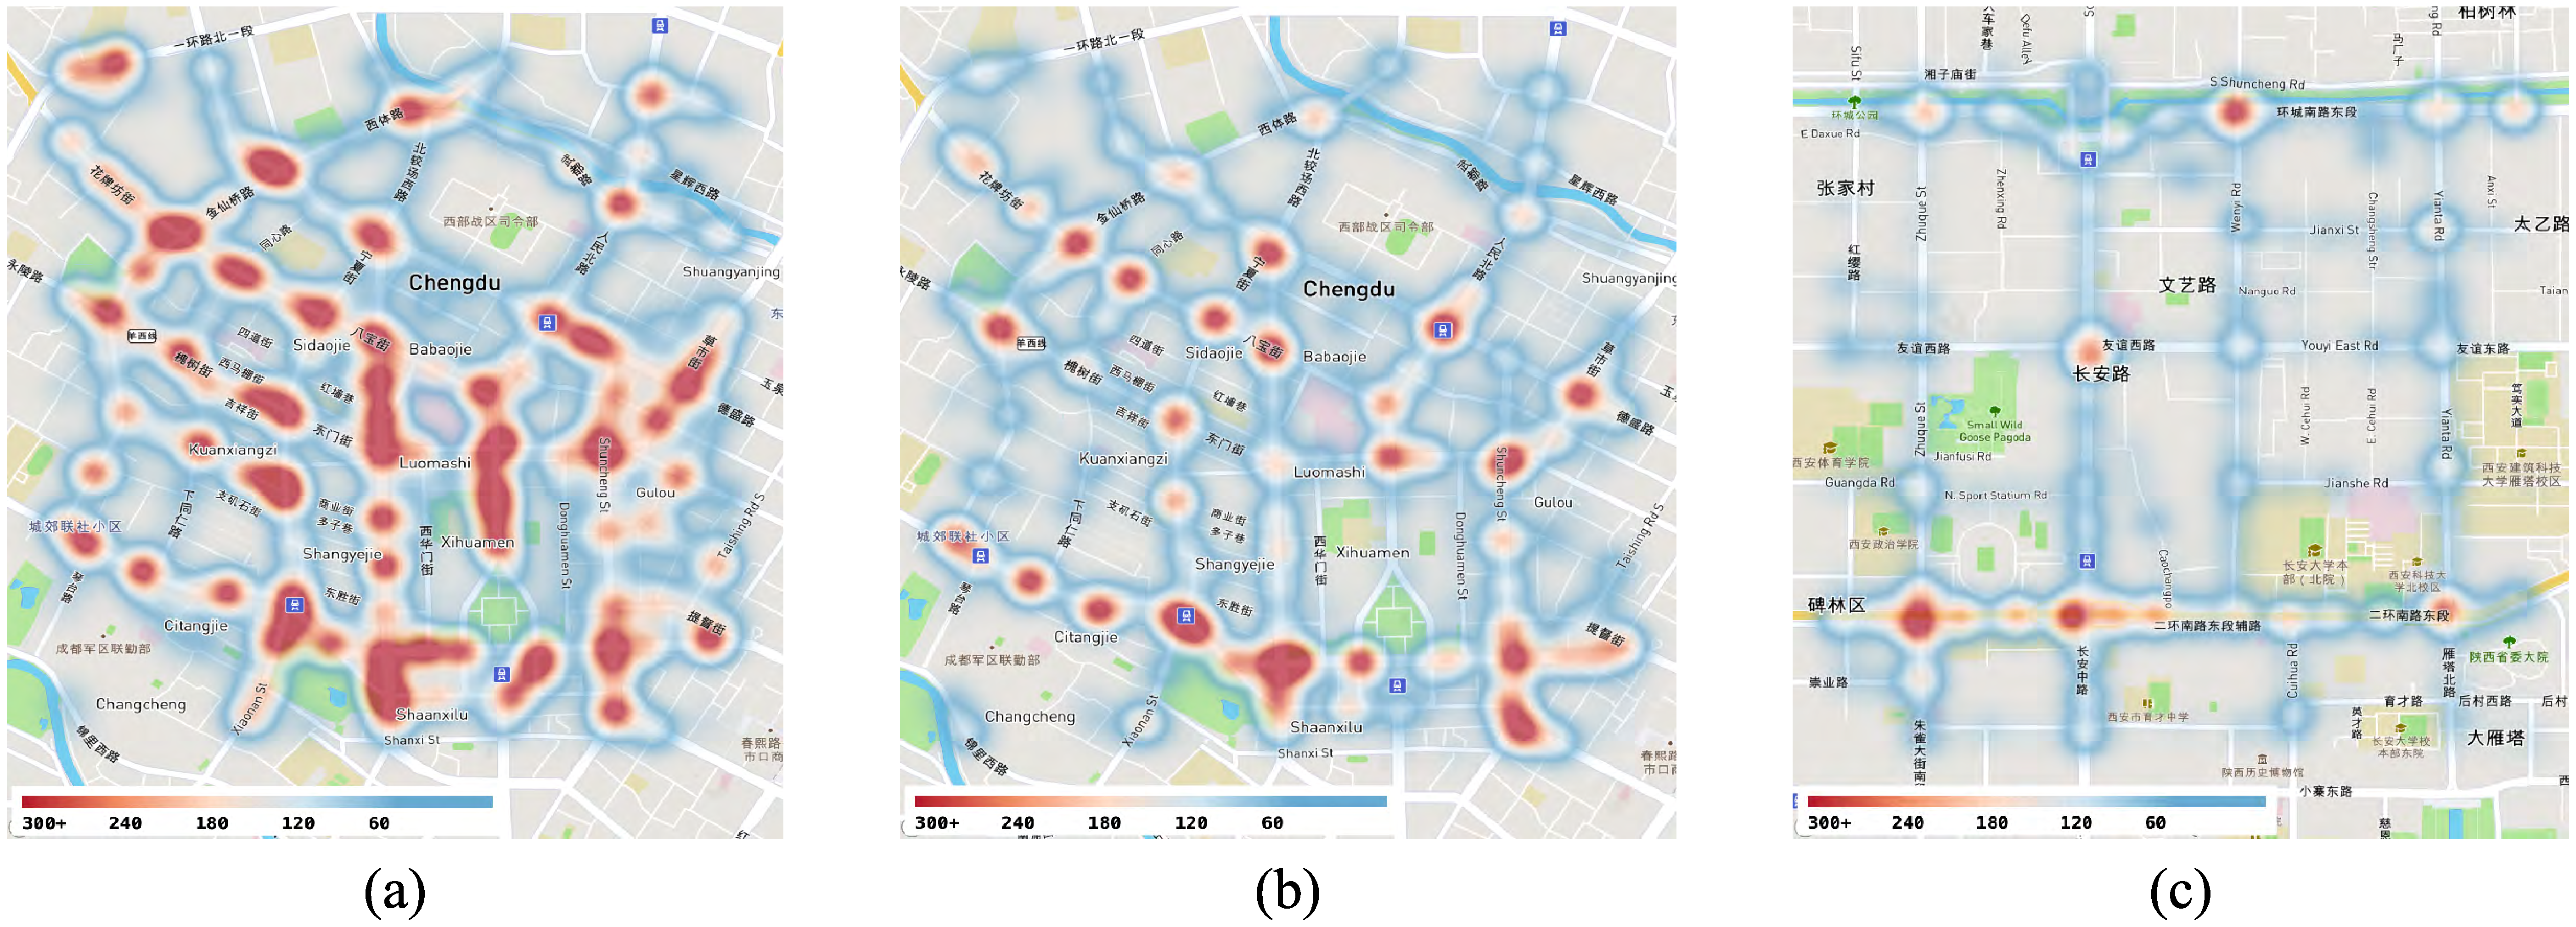
\includegraphics[width=0.5\textwidth]{fig/Fig2-5-heat-map.pdf}
	\end{figure}
\end{textblock*}
\end{center}

\begin{center}
\begin{textblock*}{\textwidth}(0cm,6.5cm)
\begin{itemize} \englishfont 
	\item[\ding{111}] {\color{cqublue}{对比算法}}
	\begin{itemize}
	\begin{small}
		\item[\ding{226}] 随机分配 ({\color{red}{RA}})、深度确定性策略梯度 ({\color{red}{DDPG}})
		\item[\ding{226}] 多智能体行动者-评论家 ({\color{red}{MAAC}})
		\item[\ding{226}] 采用VBA策略的MAAC ({\color{red}{MAAC-VBA}})
		\item
	\end{small}
	\end{itemize}
\end{itemize}
\end{textblock*}
\end{center}

\begin{center}
\begin{textblock*}{0.55\textwidth}(8.2cm,4.5cm)
\begin{itemize}[itemsep=0.2\baselineskip] \englishfont
	\item[\ding{111}] {\color{cqublue}{性能评估指标}}
	\begin{itemize}[itemsep=0.2\baselineskip]
	\begin{small}
		\item[\ding{226}] 累计奖励 ({\color{red}{CR}})
		\item[\ding{226}] 平均奖励的构成 ({\color{red}{CAR}})\\{\small{$<\frac{3}{10}(1-\hat{\Xi}_{i}),\frac{4}{10}(1-\hat{\Phi}_{i}), \frac{3}{10}(1-\hat{\Psi}_{i})>$}}
		\item[\ding{226}] 平均排队时间 ({\color{red}{AQT}})
		\item[\ding{226}] 服务率 ({\color{red}{SR}})
	\end{small}
	\end{itemize}
\end{itemize}
\end{textblock*}
\end{center}

\end{frame}

\begin{frame}
\newBackground

\begin{overlayarea}{\textwidth}{3cm}
\only<1-1>{
\frametitle{\englishfont \underline{实验}:算法收敛性}
\begin{center} \englishfont \footnotesize
\begin{textblock*}{\textwidth}(1cm,1.8cm)
	\begin{figure}
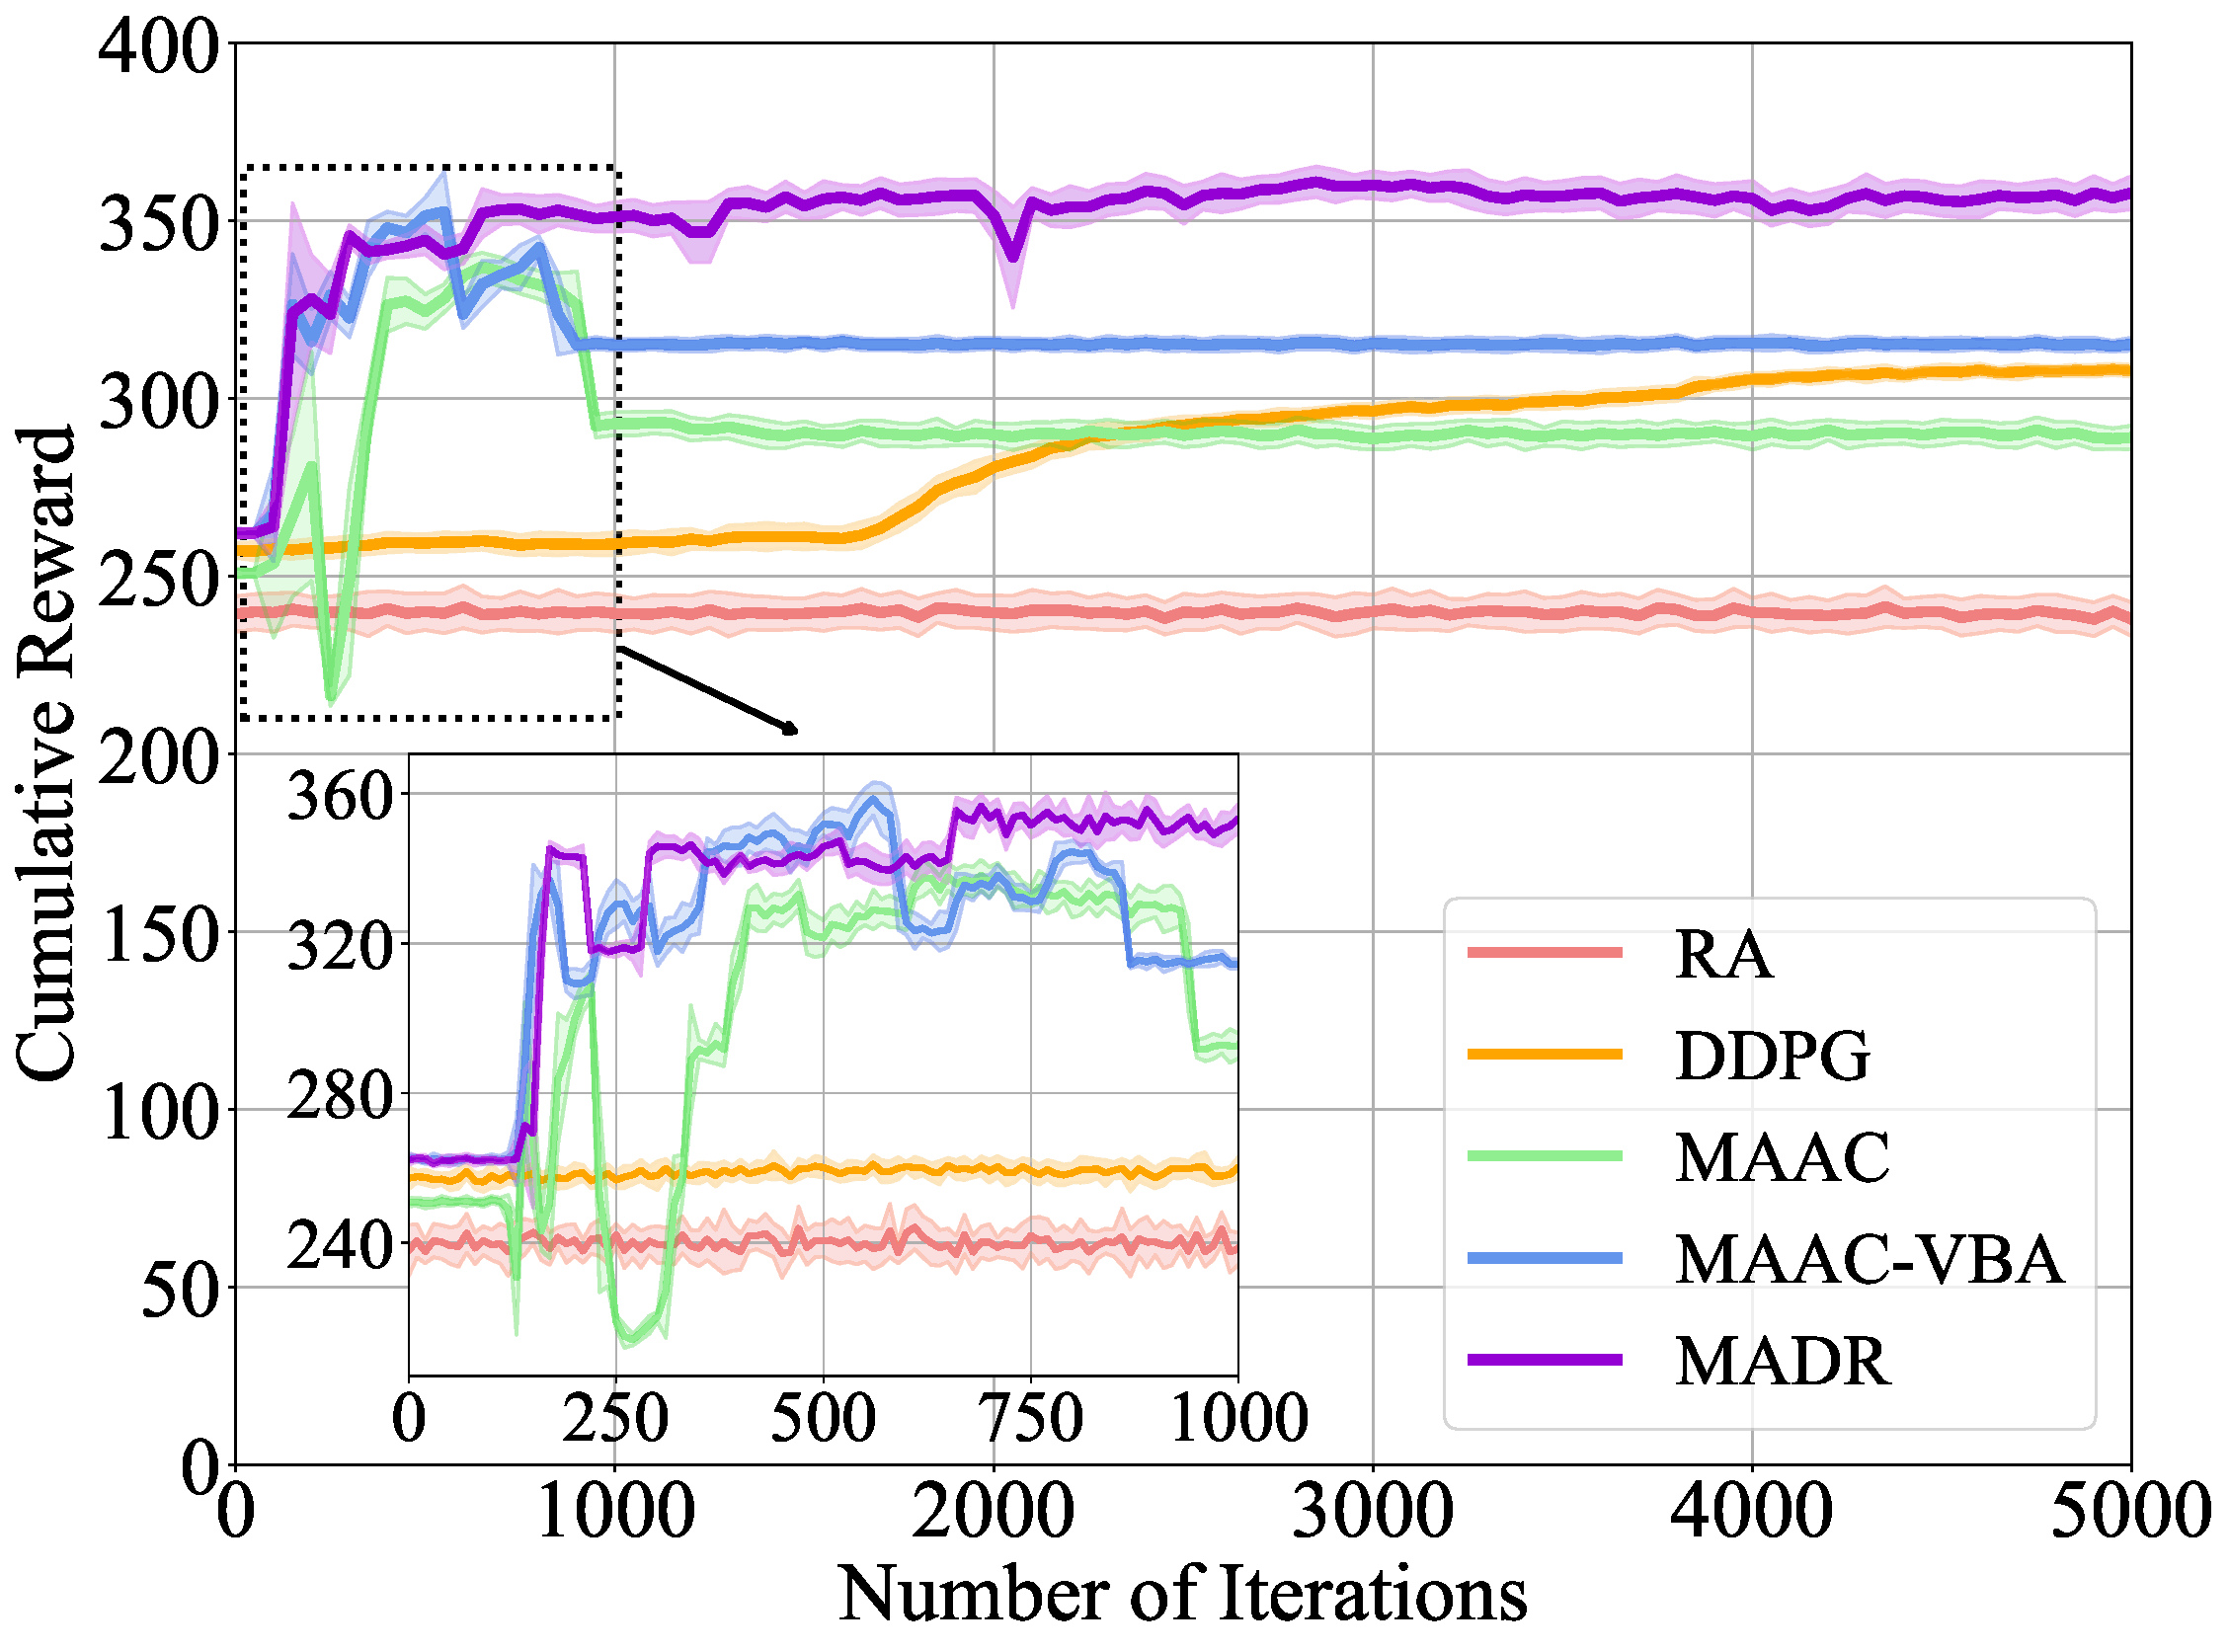
\includegraphics[width=0.6\textwidth]{fig/Fig2-6-convergence.pdf}
	\end{figure}
\end{textblock*}
\end{center}
}

\only<2-2>{
\frametitle{\englishfont \underline{实验}:算法收敛性}
\begin{center} \englishfont \footnotesize
\begin{textblock*}{\textwidth}(1cm,1.8cm)
	\begin{figure}
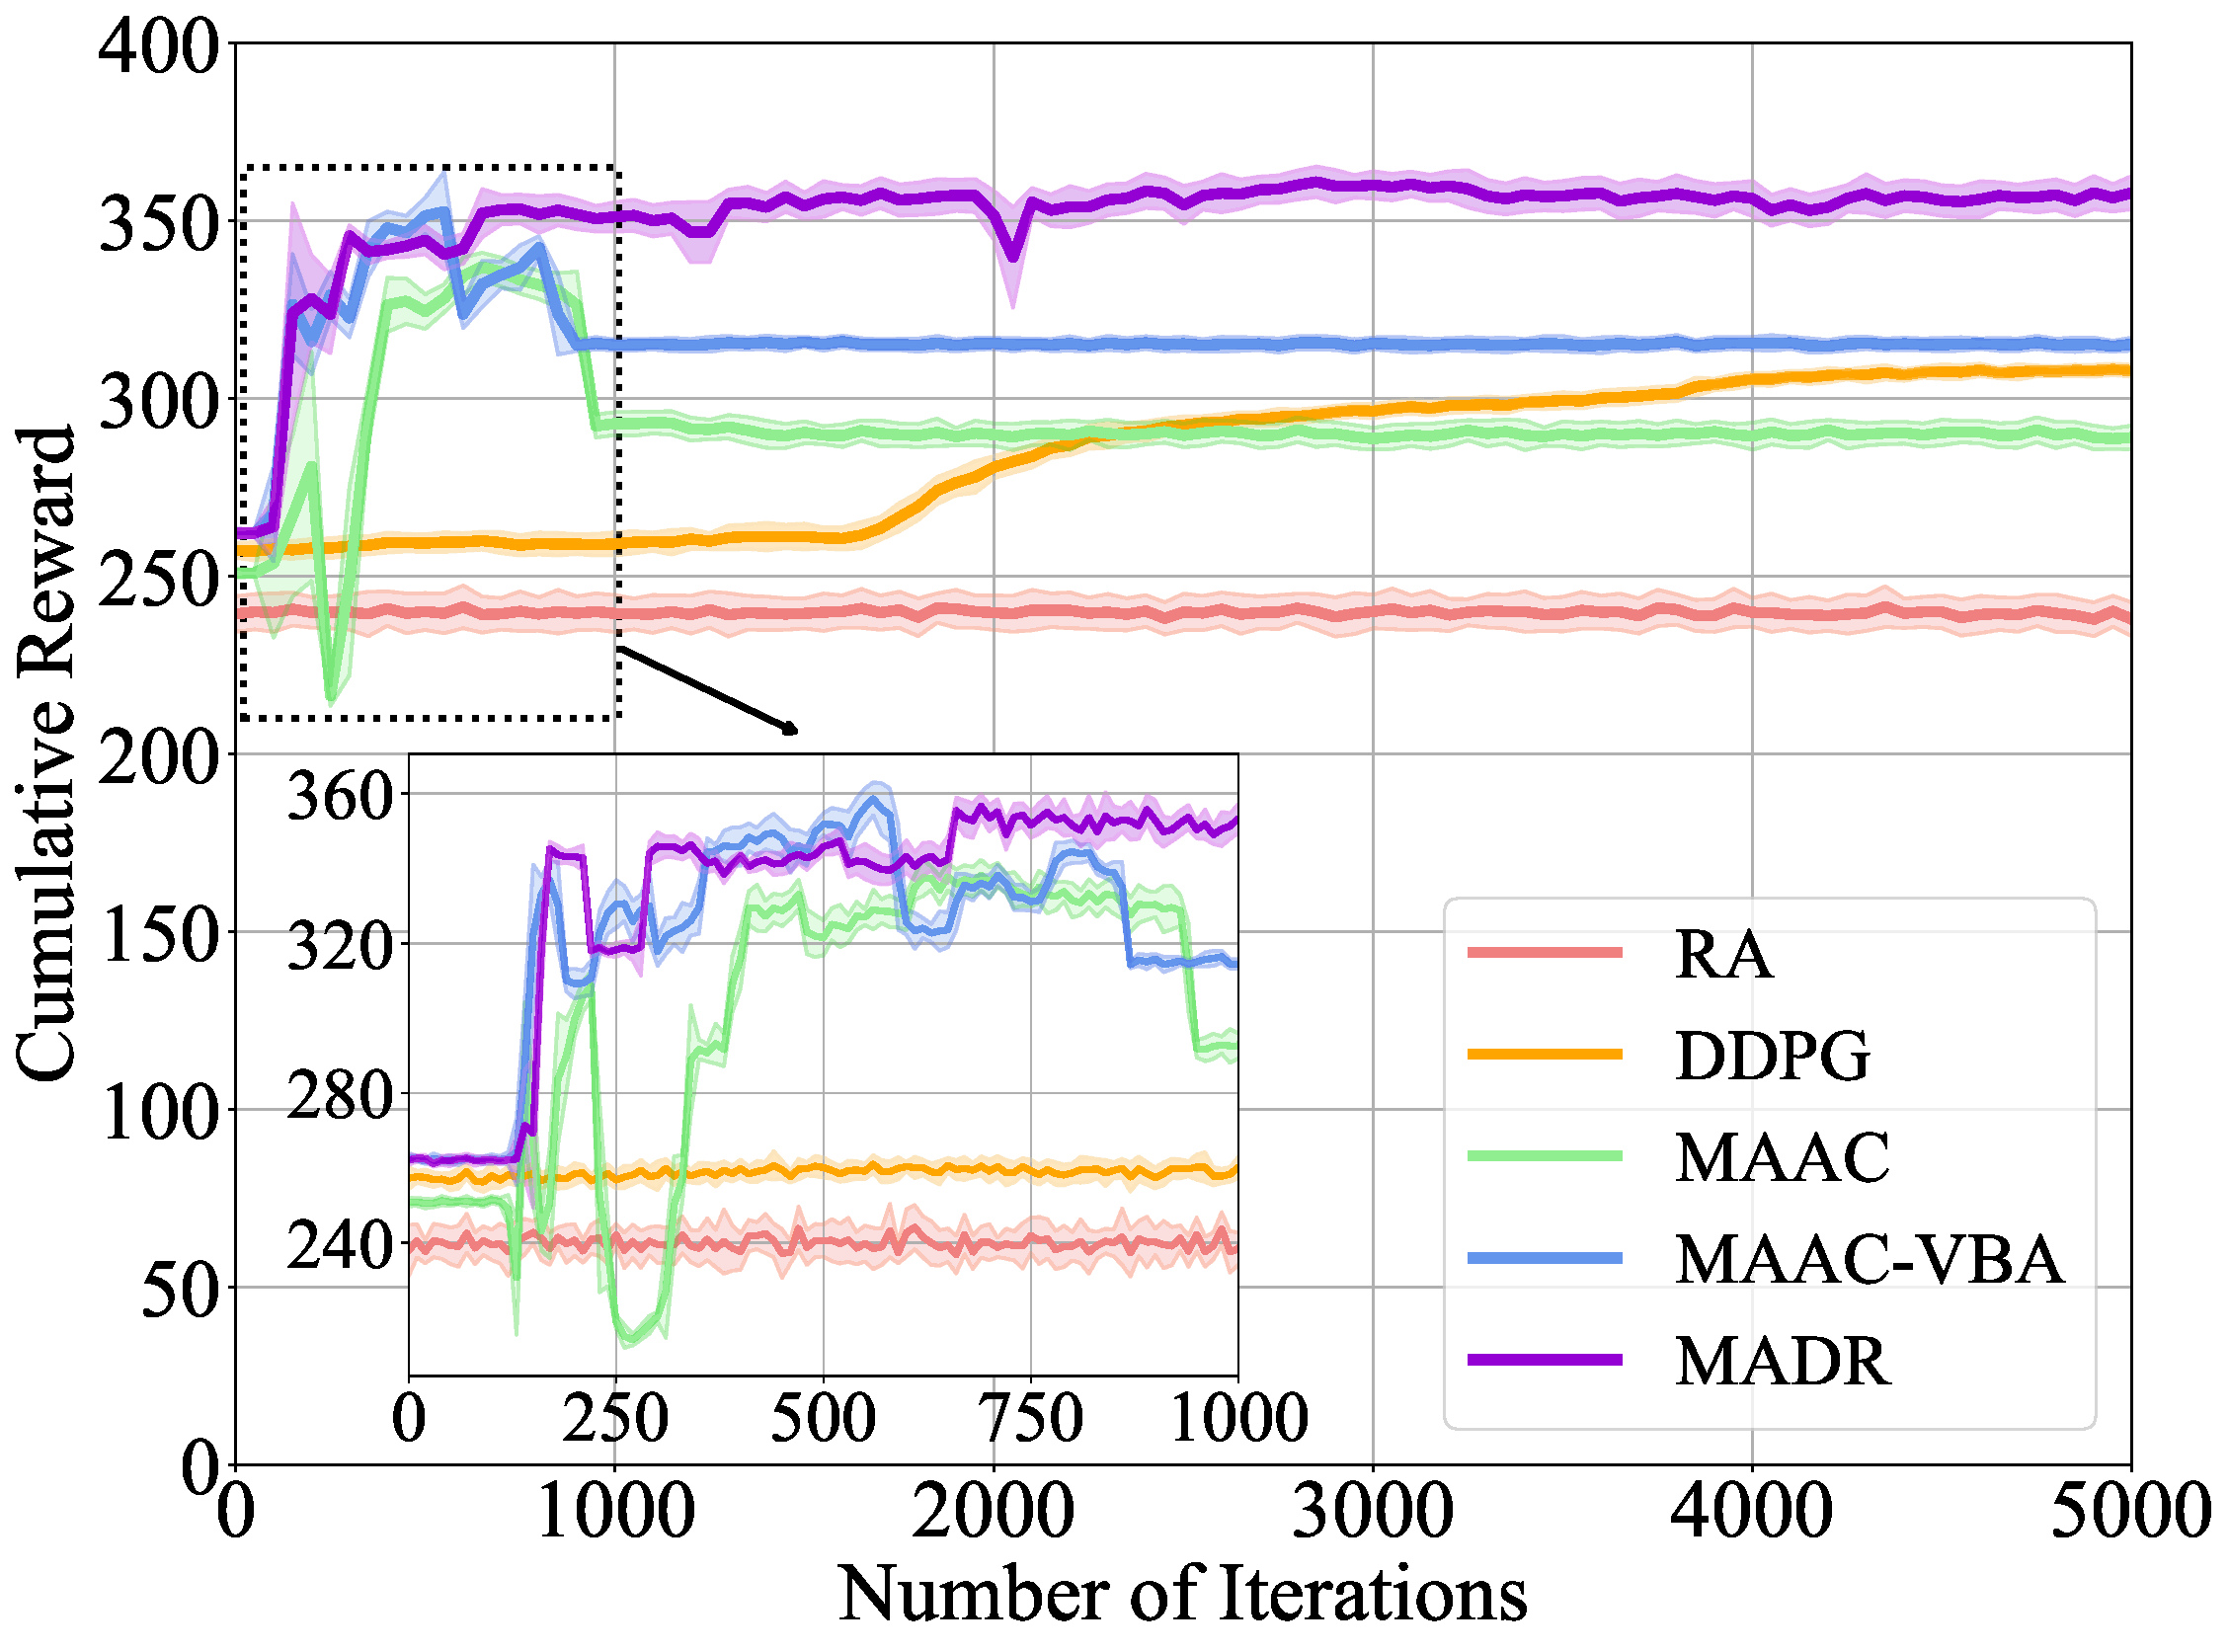
\includegraphics[width=0.6\textwidth]{fig/Fig2-6-convergence.pdf}
	\end{figure}
\end{textblock*}
\end{center}
}

\only<2-2>{
\begin{center} \englishfont \footnotesize
\begin{textblock*}{\textwidth}(1cm,1.9cm)
{\Huge{\color{red}\ding{216}}}
\end{textblock*}
\end{center}
}

\only<3-3>{
\frametitle{\englishfont \underline{实验}:交通场景的影响}
\begin{center} \englishfont \footnotesize
\begin{textblock*}{\textwidth}(1cm,1.8cm)
	\begin{figure}
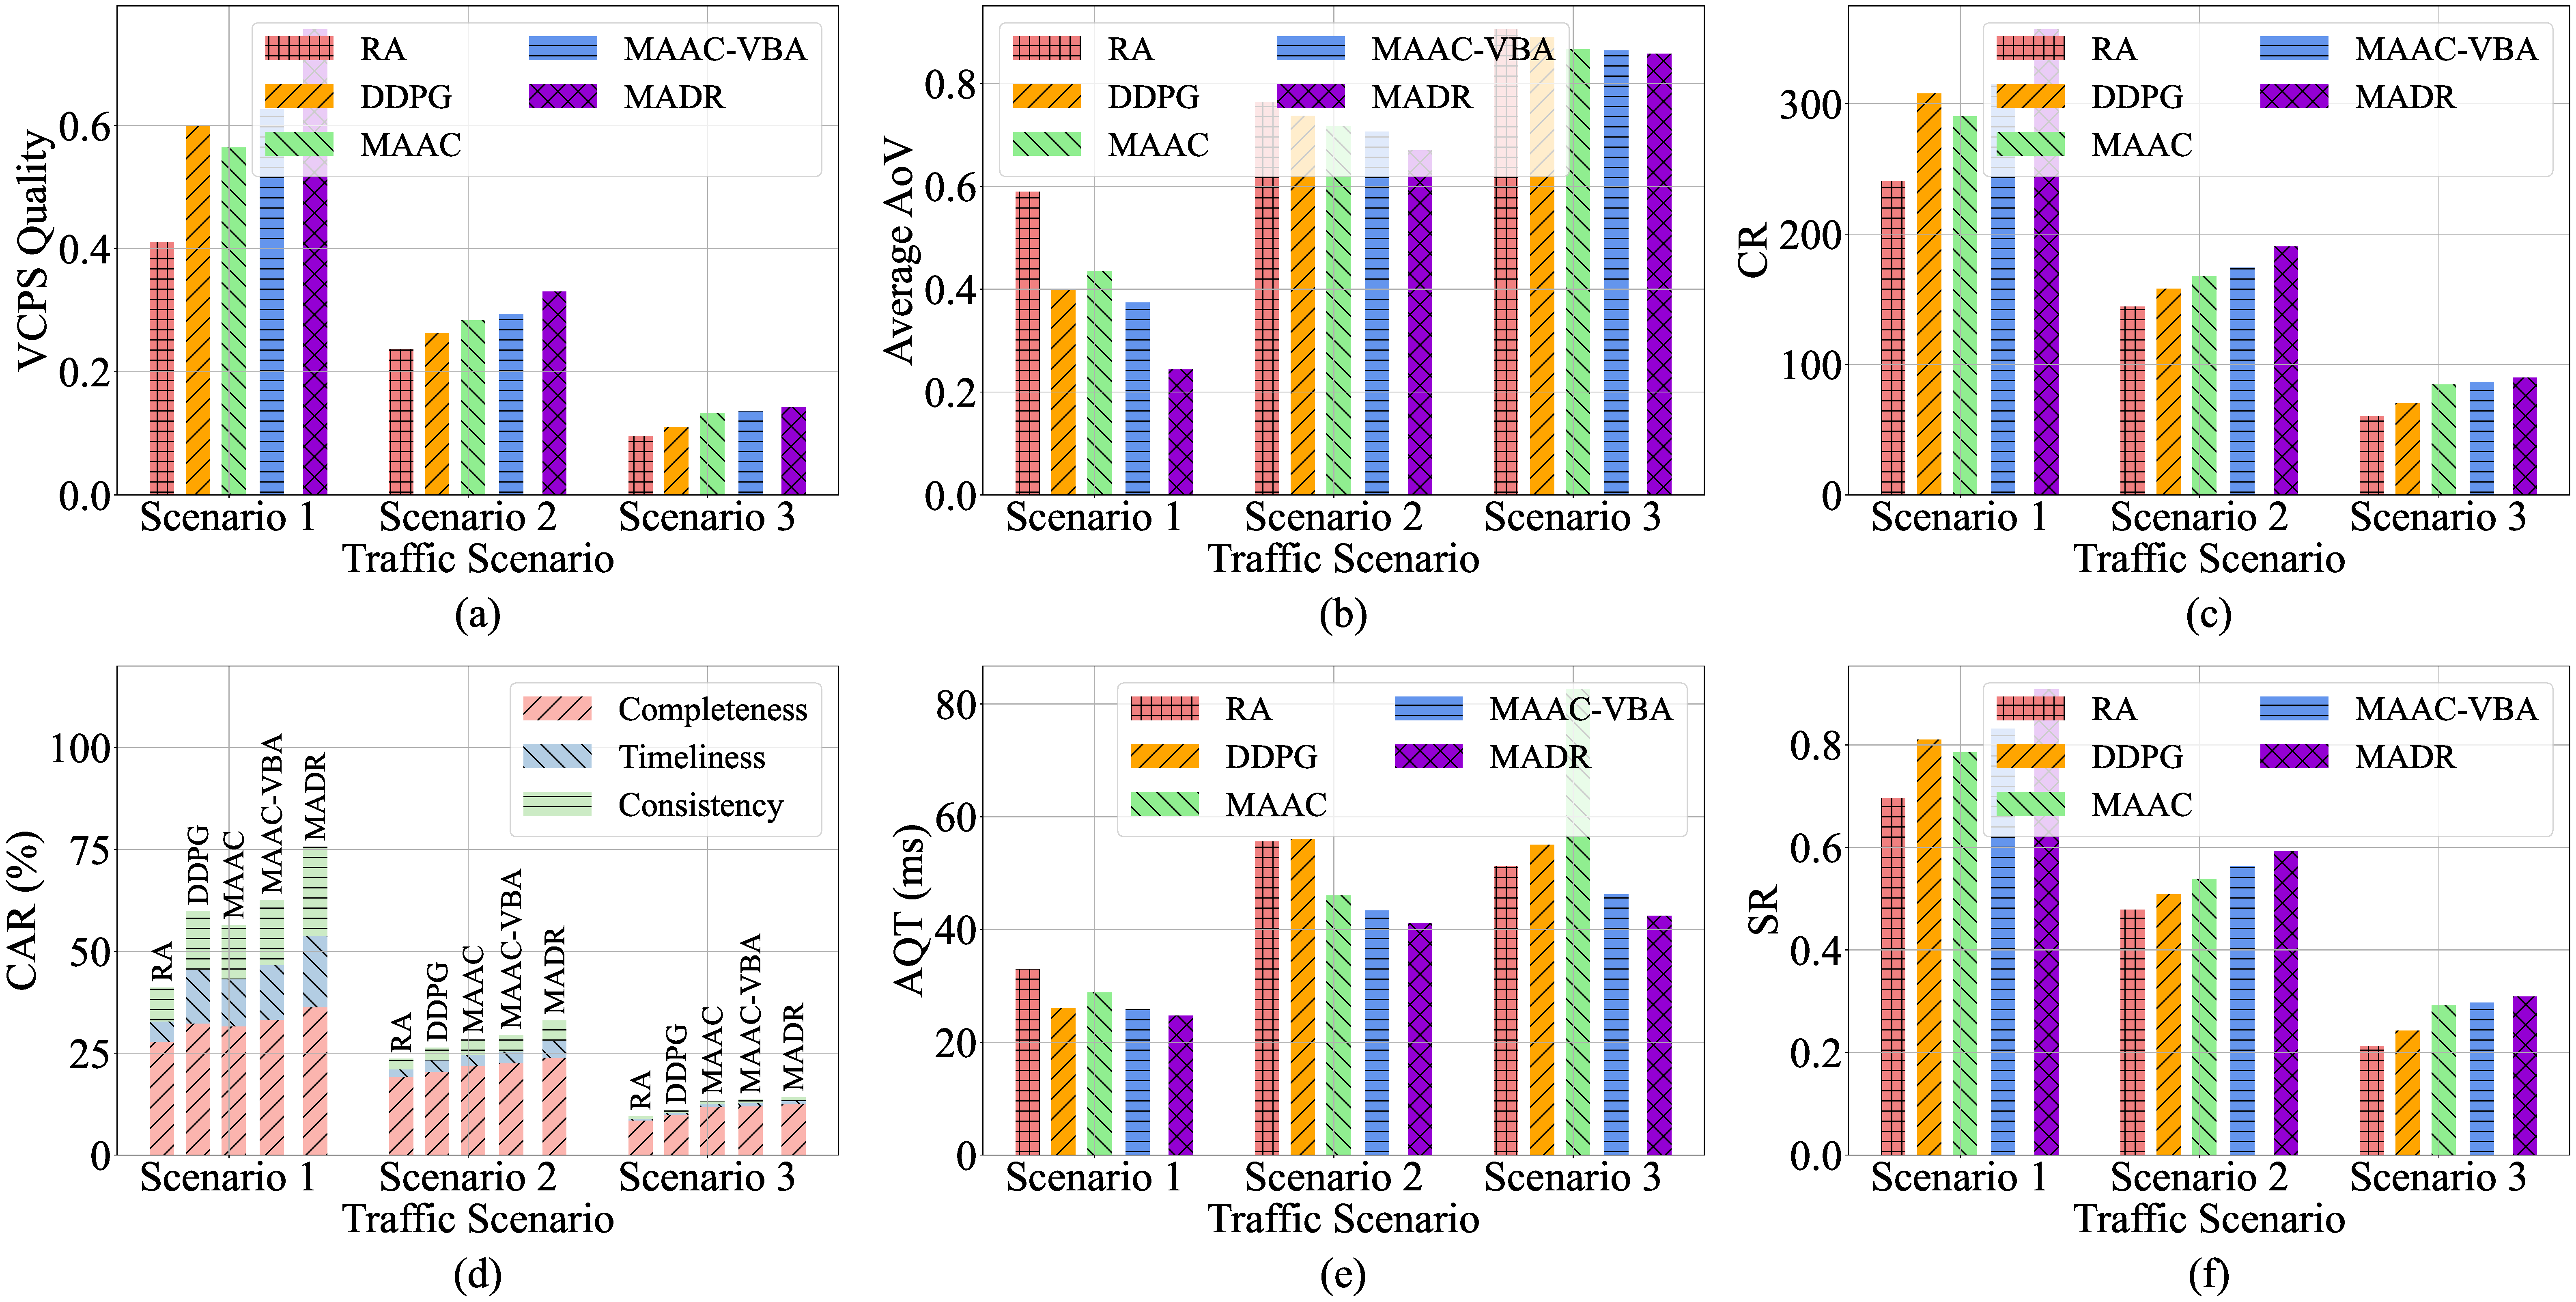
\includegraphics[width=0.9\textwidth]{fig/Fig2-7-different-scenarios.pdf}
	\end{figure}
\end{textblock*}
\end{center}
}

\only<4-4>{
\frametitle{\englishfont \underline{实验}:交通场景的影响}
\begin{center} \englishfont \footnotesize
\begin{textblock*}{\textwidth}(1cm,1.8cm)
	\begin{figure}
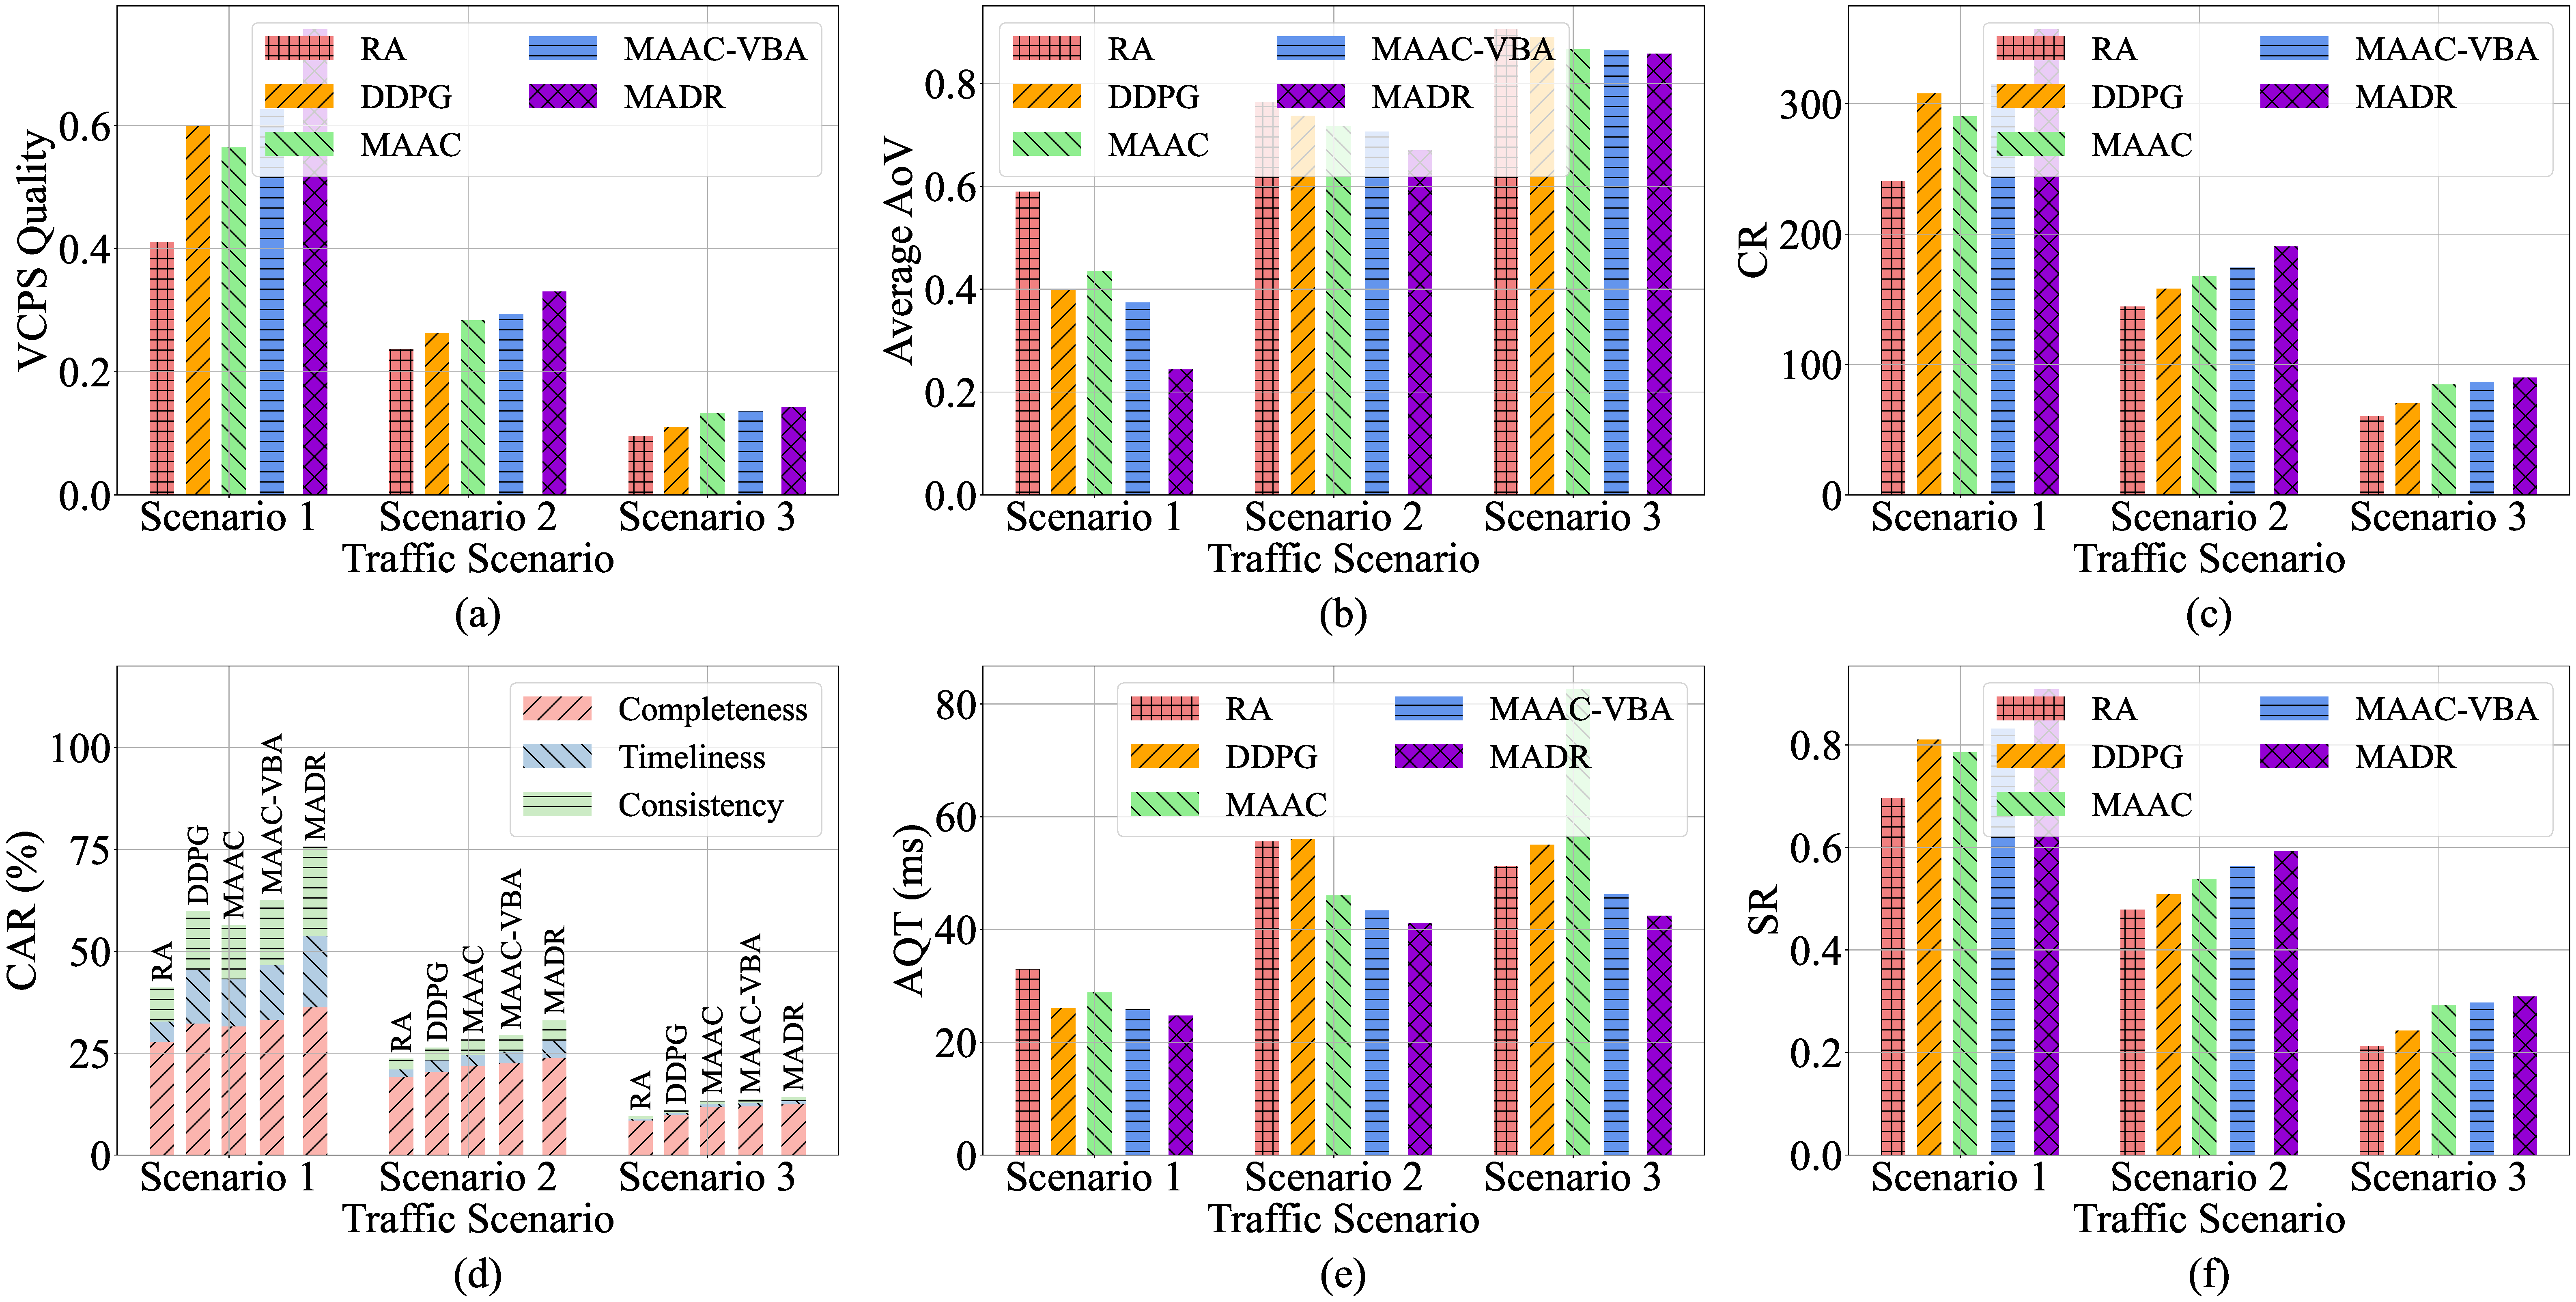
\includegraphics[width=0.9\textwidth]{fig/Fig2-7-different-scenarios.pdf}
	\end{figure}
\end{textblock*}
\end{center}
}

\only<4-4>{
\begin{center} \englishfont \footnotesize
\begin{textblock*}{\textwidth}(-1.6cm,3.4cm)
{\LARGE{\color{red}\ding{216}}}
\end{textblock*}
\end{center}

\begin{center} \englishfont \footnotesize
\begin{textblock*}{\textwidth}(0.3cm,3.25cm)
{\LARGE{\color{red}\ding{216}}}
\end{textblock*}
\end{center}

\begin{center} \englishfont \footnotesize
\begin{textblock*}{\textwidth}(5.7cm,2.65cm)
{\LARGE{\color{red}\ding{216}}}
\end{textblock*}
\end{center}

\begin{center} \englishfont \footnotesize
\begin{textblock*}{\textwidth}(2.6cm,5.9cm)
{\LARGE{\color{red}\ding{216}}}
\end{textblock*}
\end{center}

\begin{center} \englishfont \footnotesize
\begin{textblock*}{\textwidth}(6.85cm,6.3cm)
{\LARGE{\color{red}\ding{216}}}
\end{textblock*}
\end{center}
}

\only<5-5>{
\frametitle{\englishfont \underline{实验}:V2I带宽的影响}
\begin{center} \englishfont \footnotesize
\begin{textblock*}{\textwidth}(1cm,1.8cm)
	\begin{figure}
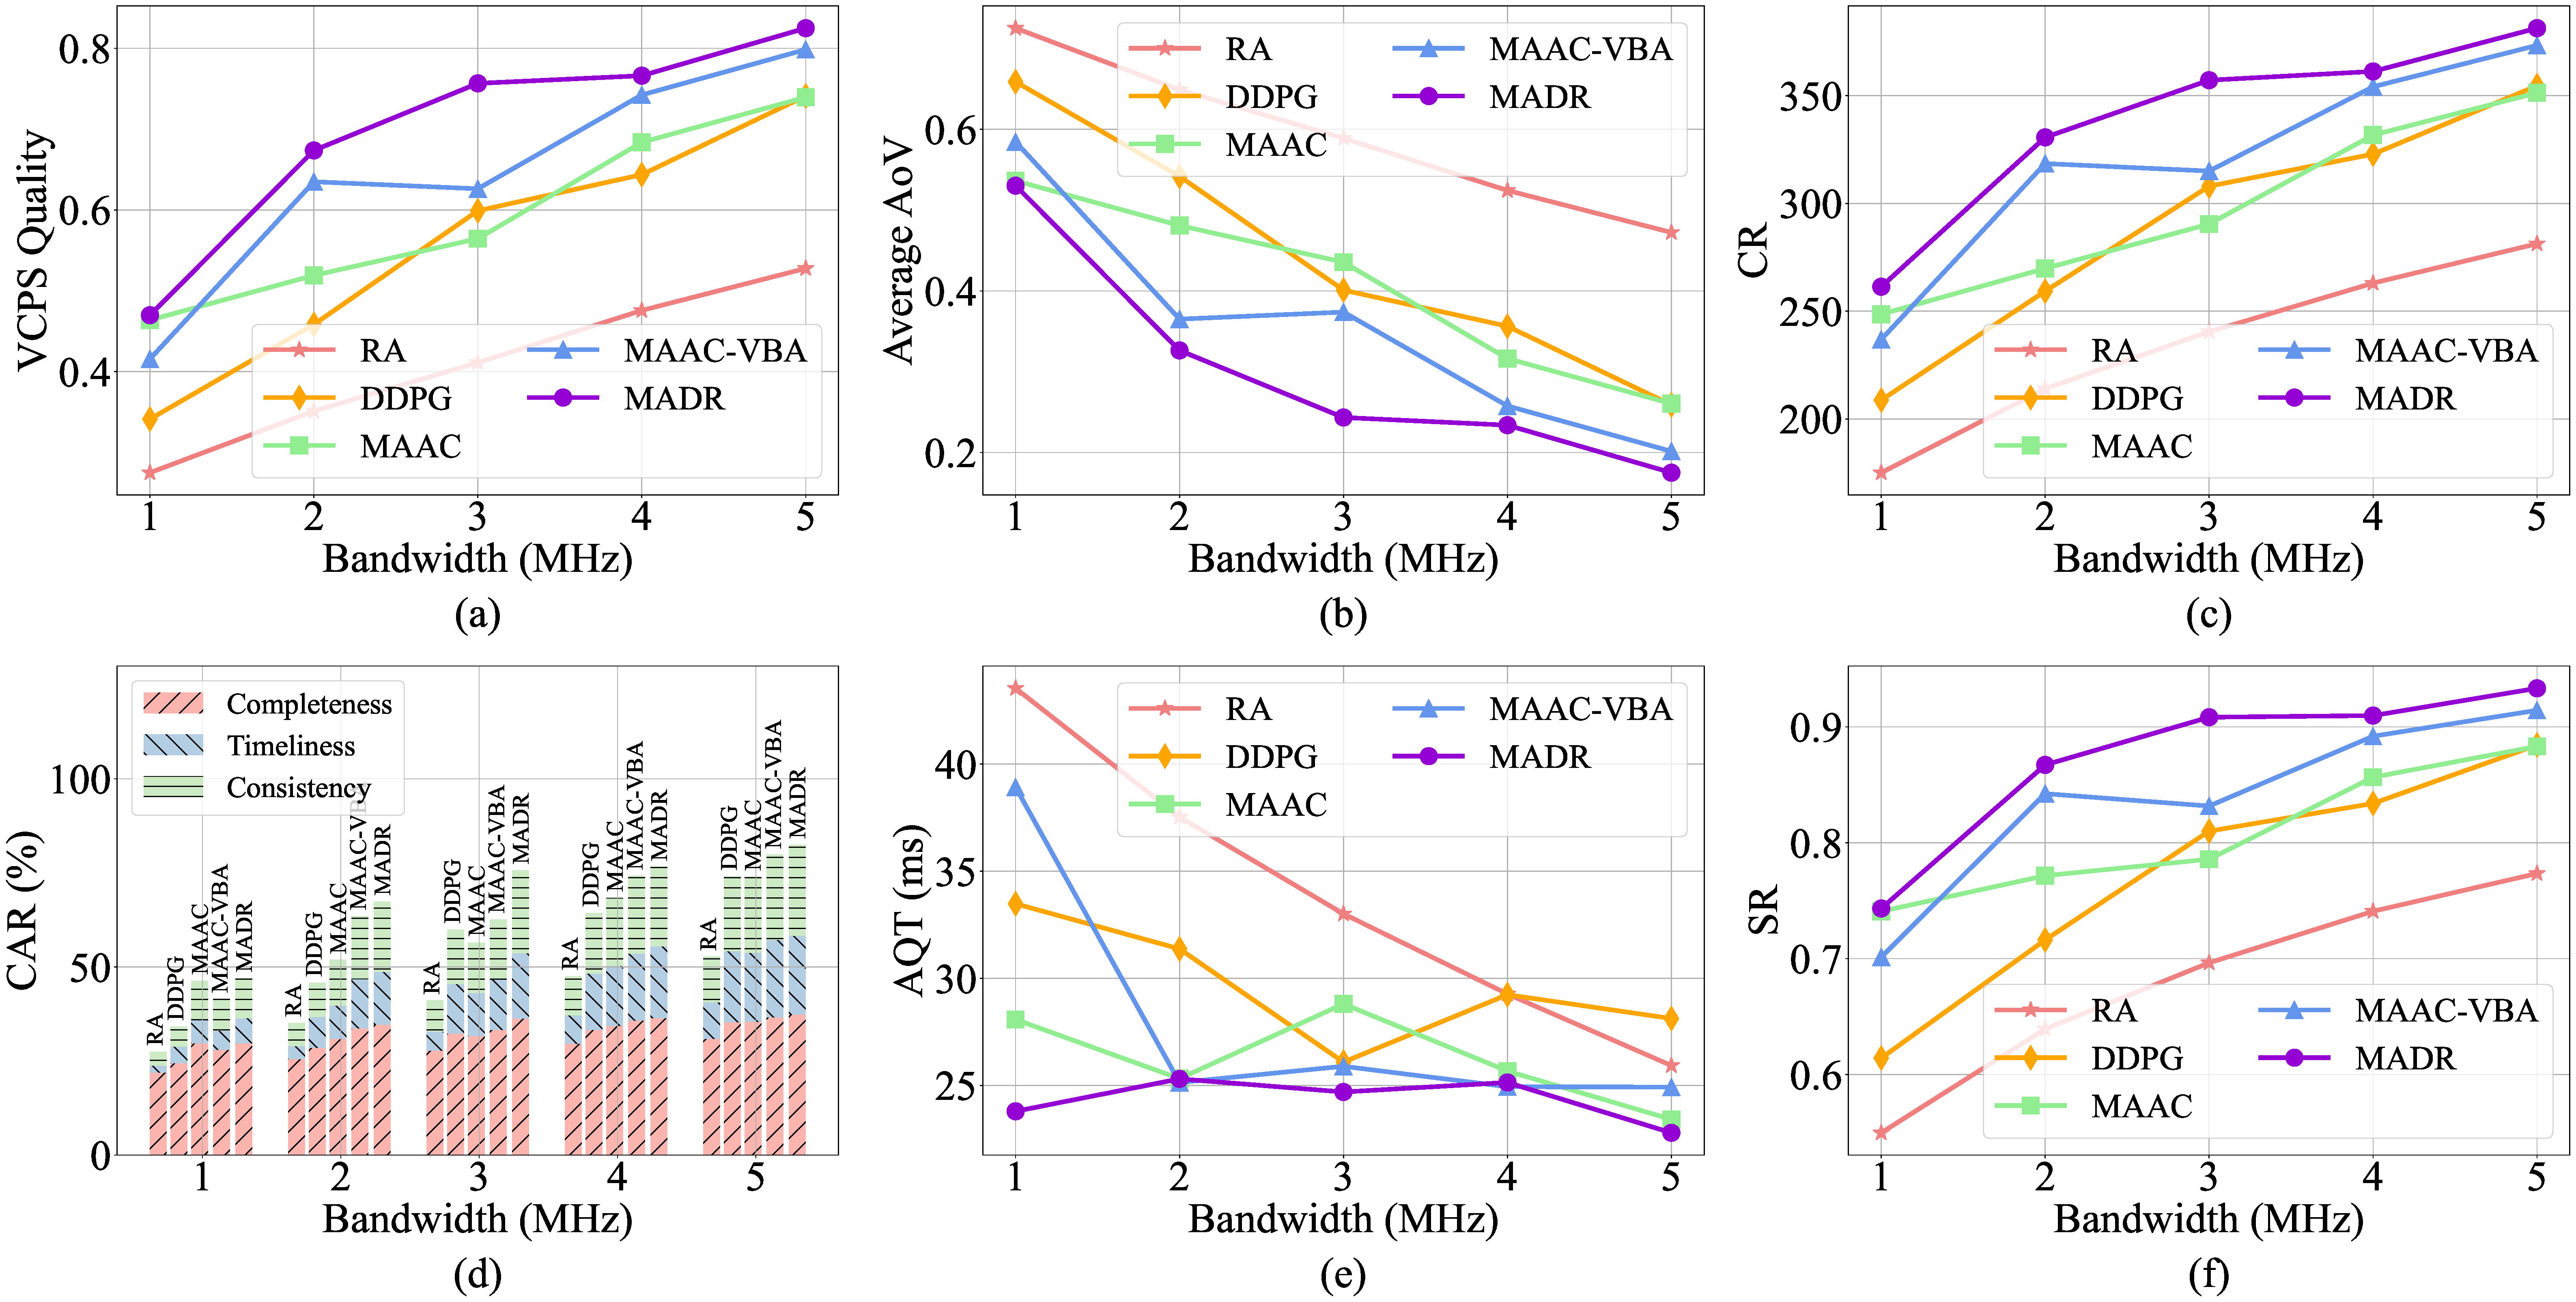
\includegraphics[width=0.9\textwidth]{fig/Fig2-8-different-bandwidths.pdf}
	\end{figure}
\end{textblock*}
\end{center}
}

\only<6-6>{
\frametitle{\englishfont \underline{实验}:V2I带宽的影响}
\begin{center} \englishfont \footnotesize
\begin{textblock*}{\textwidth}(1cm,1.8cm)
	\begin{figure}
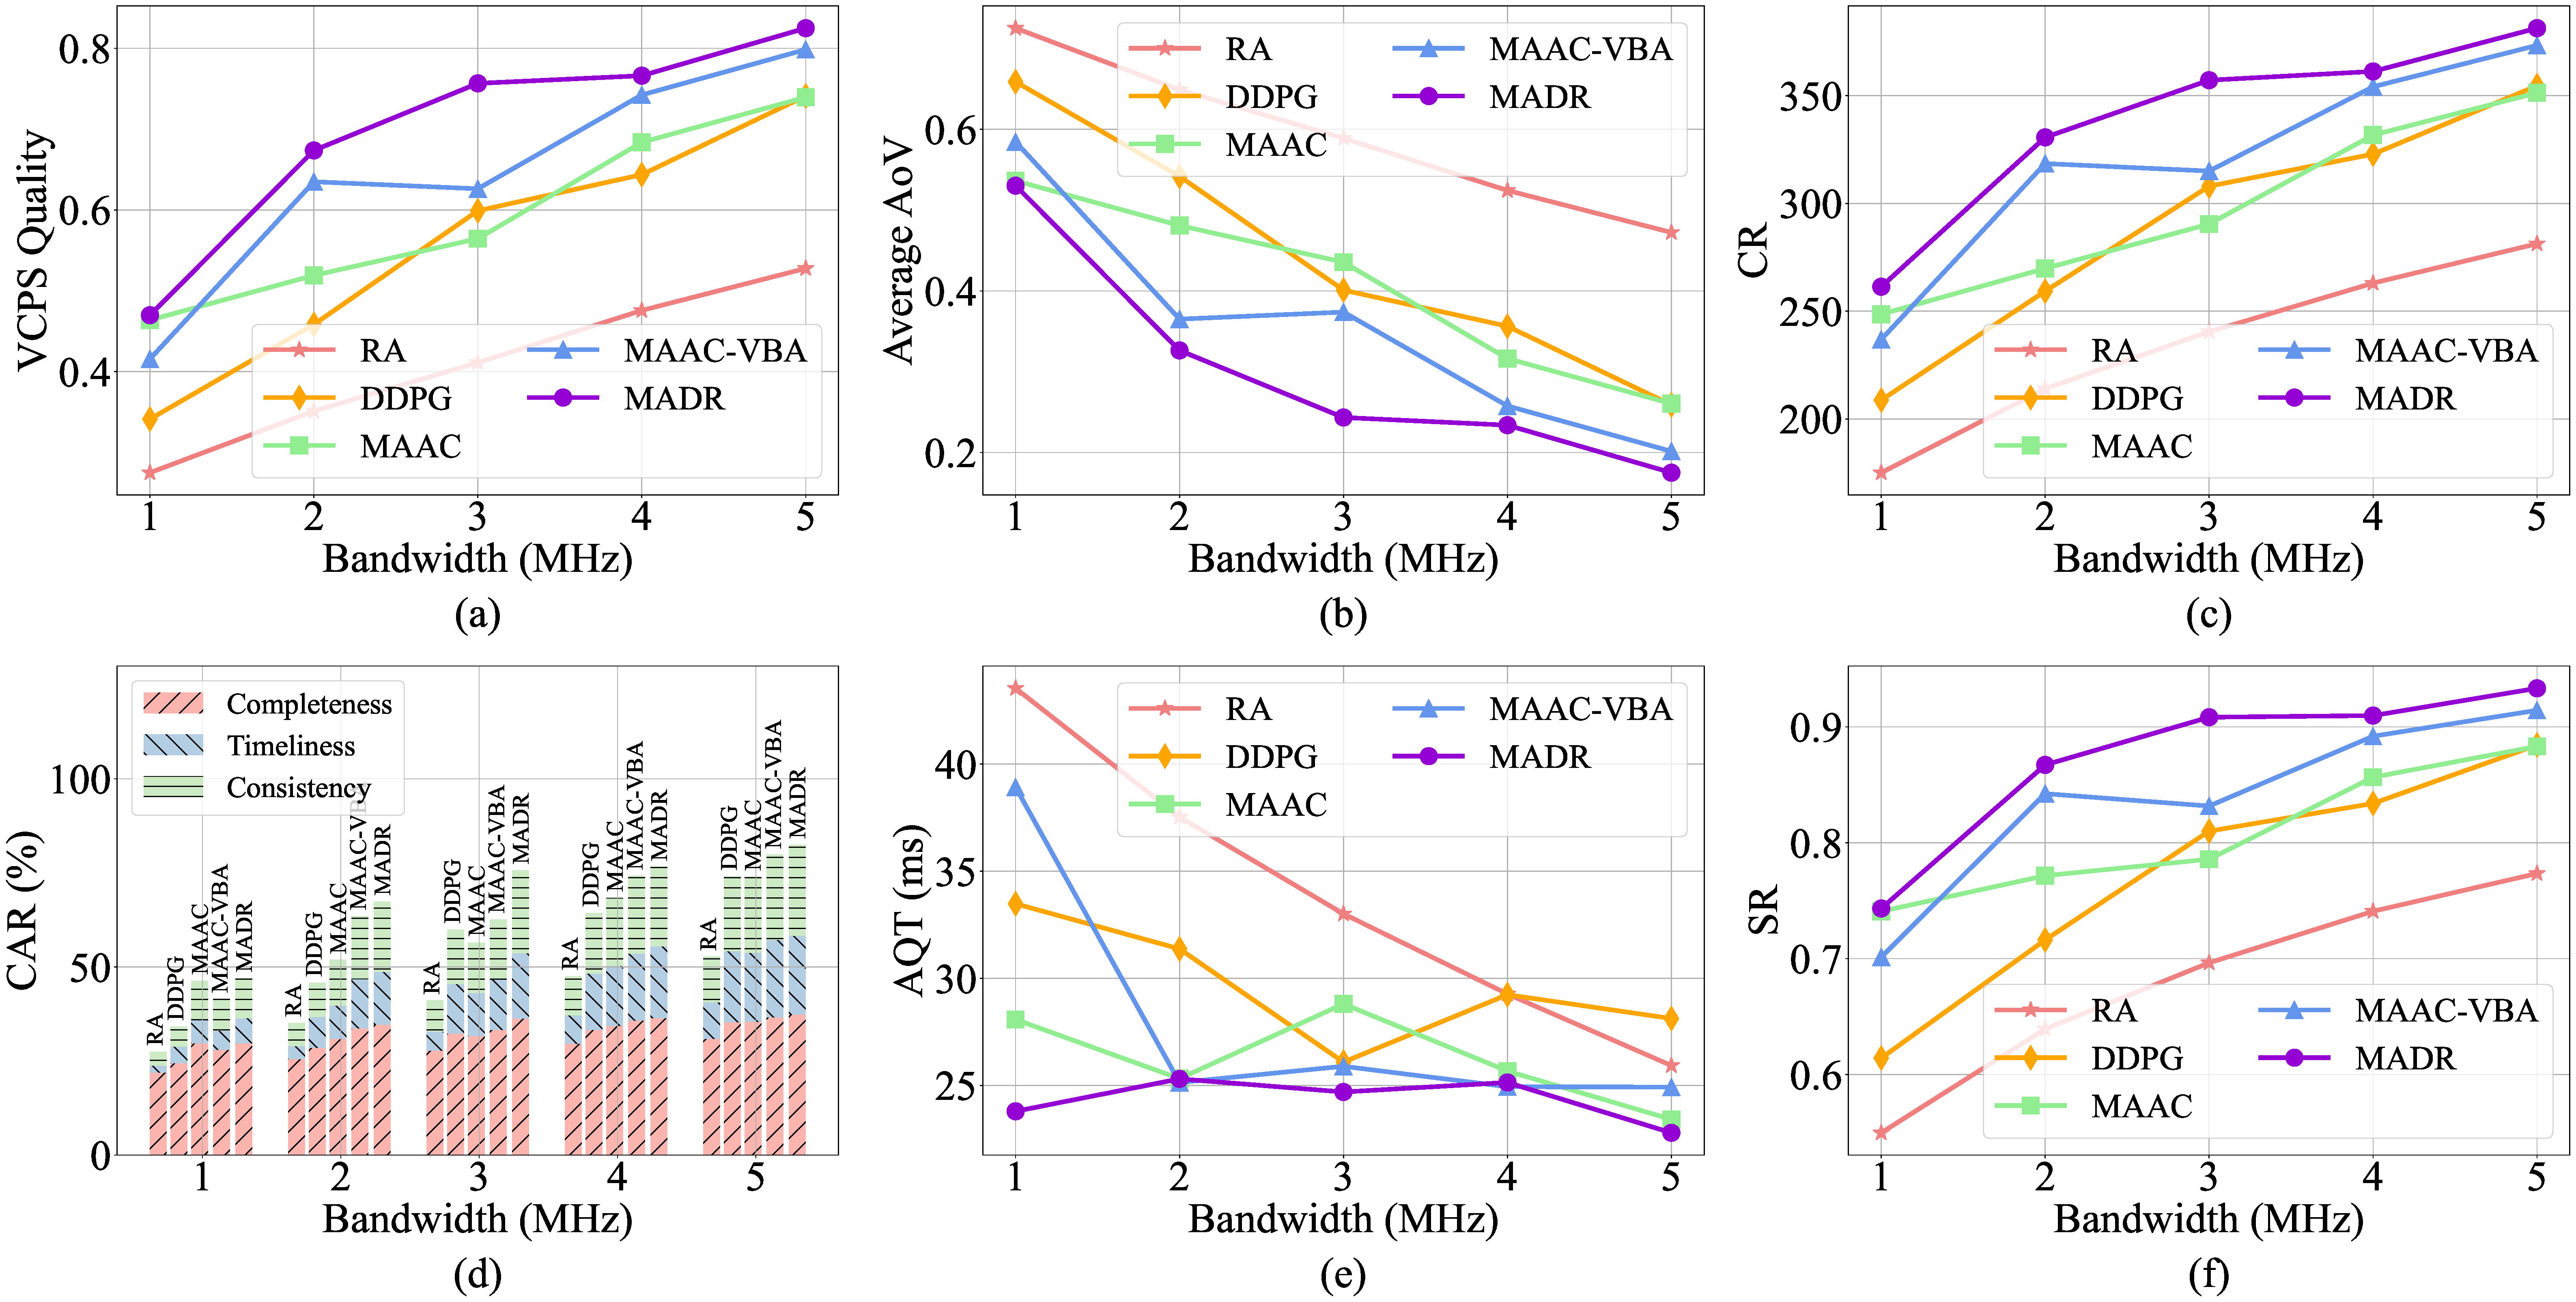
\includegraphics[width=0.9\textwidth]{fig/Fig2-8-different-bandwidths.pdf}
	\end{figure}
\end{textblock*}
\end{center}
}

\only<6-6>{
\begin{center} \englishfont \footnotesize
\begin{textblock*}{\textwidth}(-2.6cm,1.8cm)
{\LARGE{\color{red}\ding{216}}}
\end{textblock*}
\end{center}

\begin{center} \englishfont \footnotesize
\begin{textblock*}{\textwidth}(1cm,3.35cm)
{\LARGE{\color{red}\ding{216}}}
\end{textblock*}
\end{center}

\begin{center} \englishfont \footnotesize
\begin{textblock*}{\textwidth}(5.7cm,1.7cm)
{\LARGE{\color{red}\ding{216}}}
\end{textblock*}
\end{center}

\begin{center} \englishfont \footnotesize
\begin{textblock*}{\textwidth}(0.85cm,6.8cm)
{\LARGE{\color{red}\ding{216}}}
\end{textblock*}
\end{center}

\begin{center} \englishfont \footnotesize
\begin{textblock*}{\textwidth}(5.65cm,4.9cm)
{\LARGE{\color{red}\ding{216}}}
\end{textblock*}
\end{center}
}

\only<7-7>{
\frametitle{\englishfont \underline{实验}:视图需求的影响}
\begin{center} \englishfont \footnotesize
\begin{textblock*}{\textwidth}(1cm,1.8cm)
	\begin{figure}
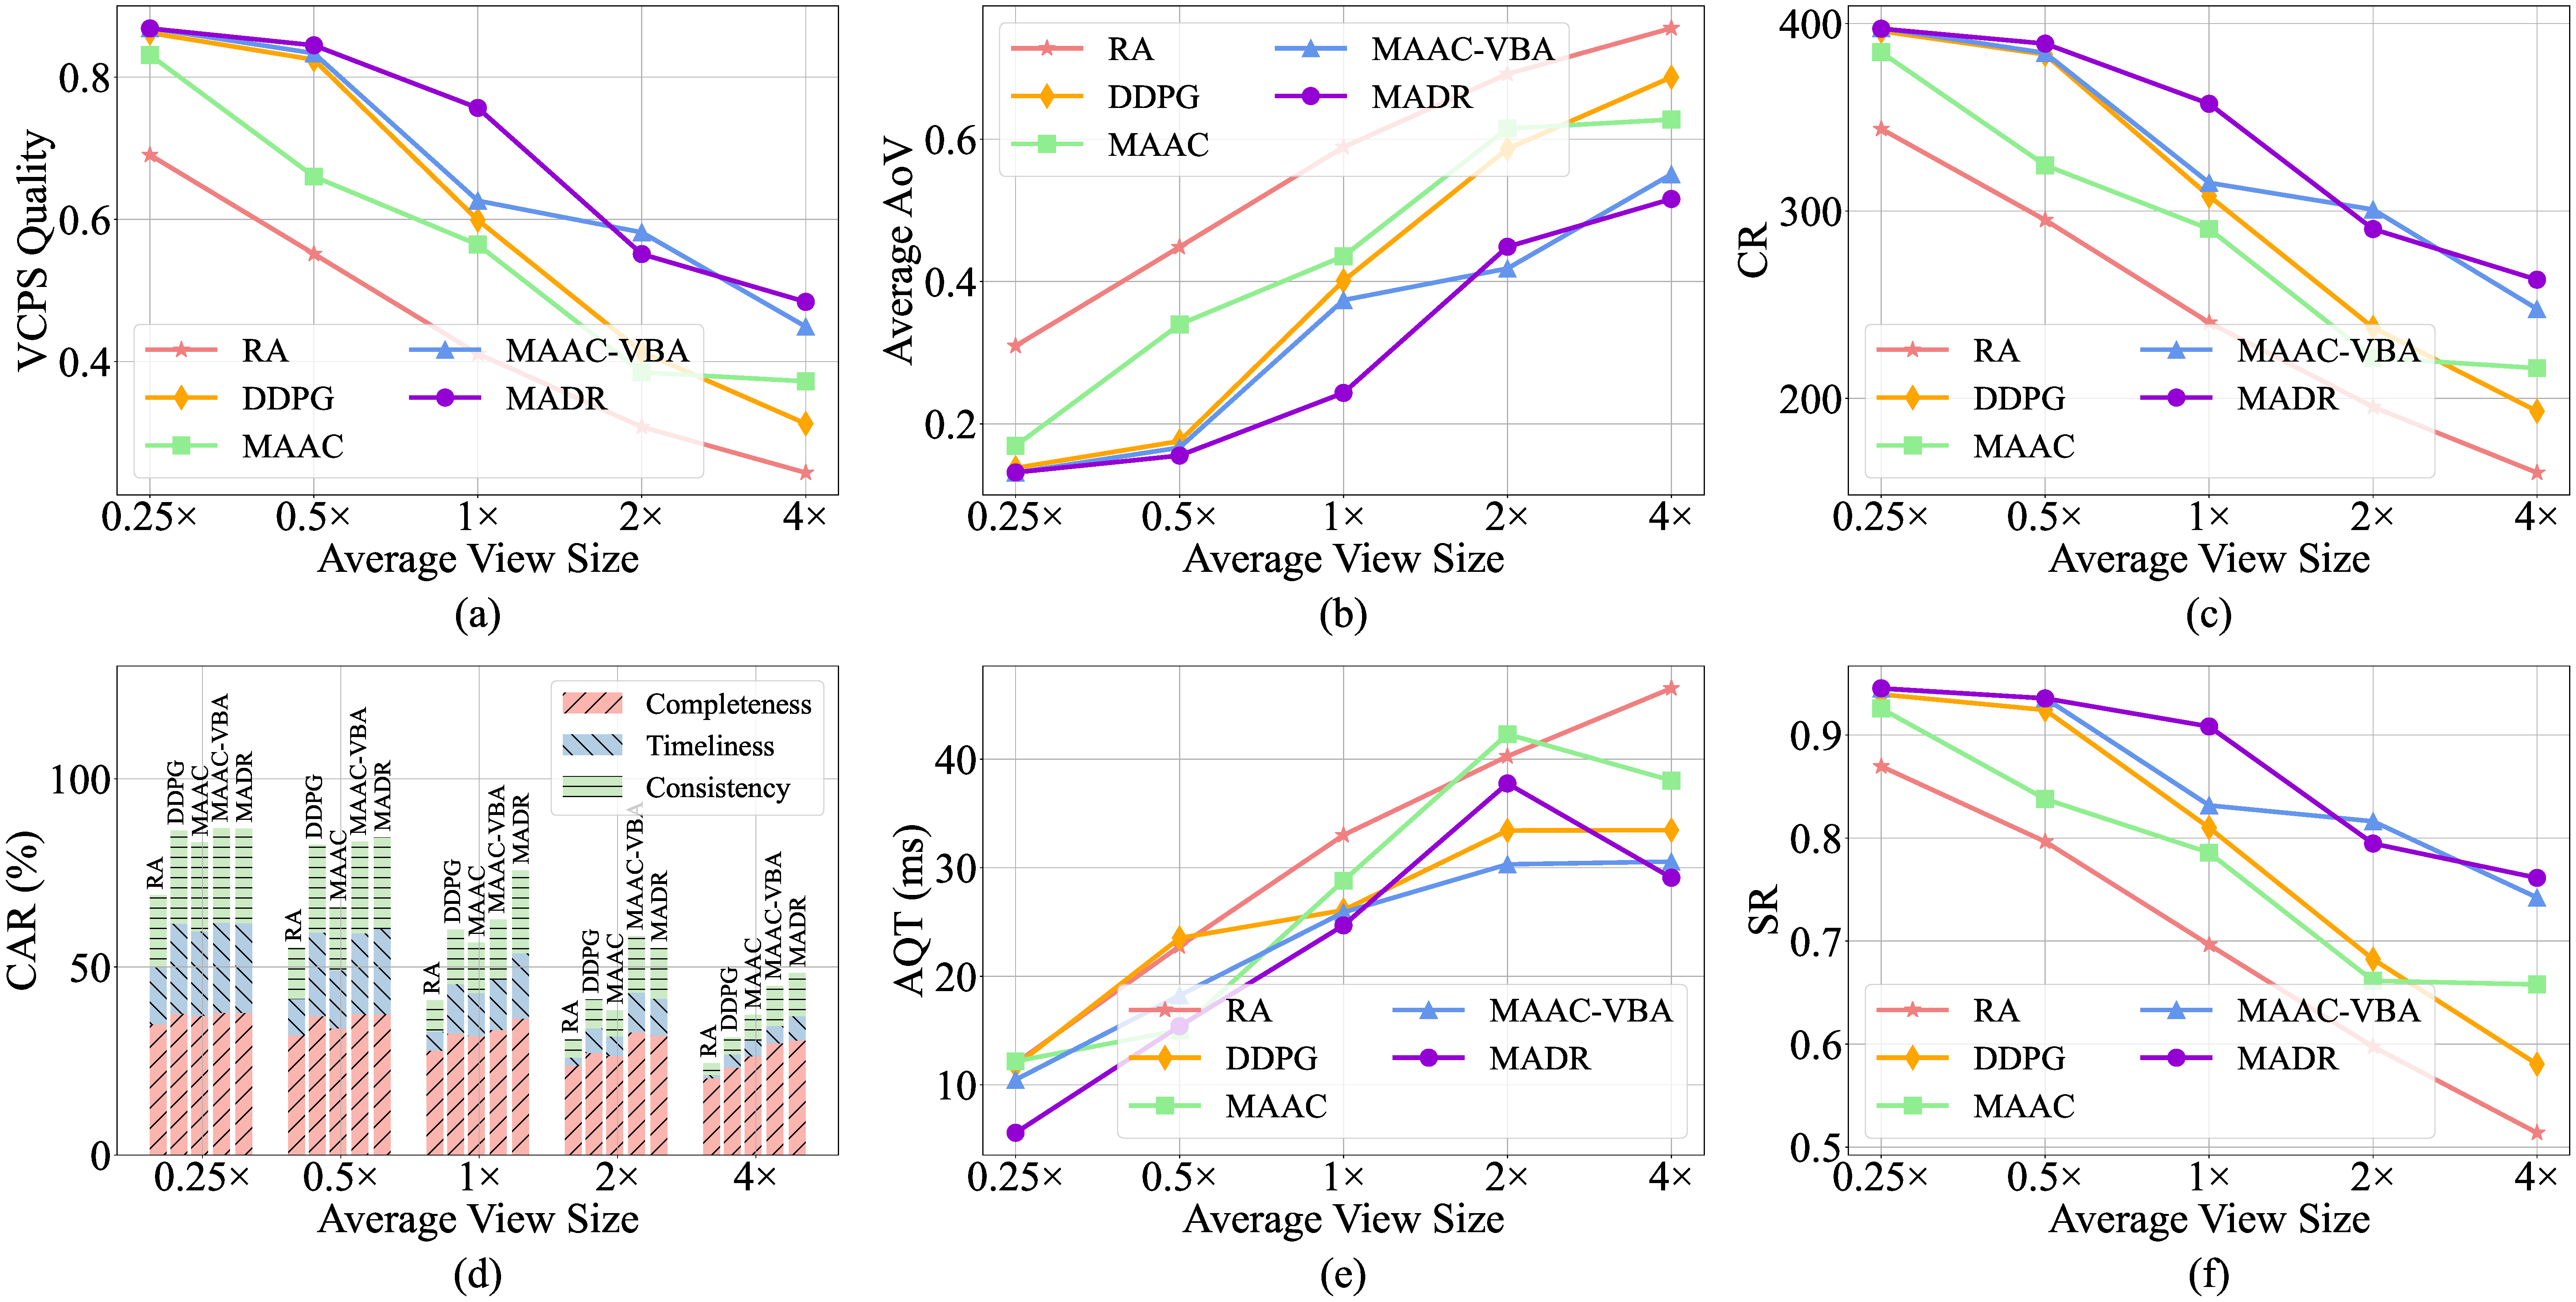
\includegraphics[width=0.9\textwidth]{fig/Fig2-9-different-view-sizes.pdf}
	\end{figure}
\end{textblock*}
\end{center}
}

\only<8-8>{
\frametitle{\englishfont \underline{实验}:视图需求的影响}
\begin{center} \englishfont \footnotesize
\begin{textblock*}{\textwidth}(1cm,1.8cm)
	\begin{figure}
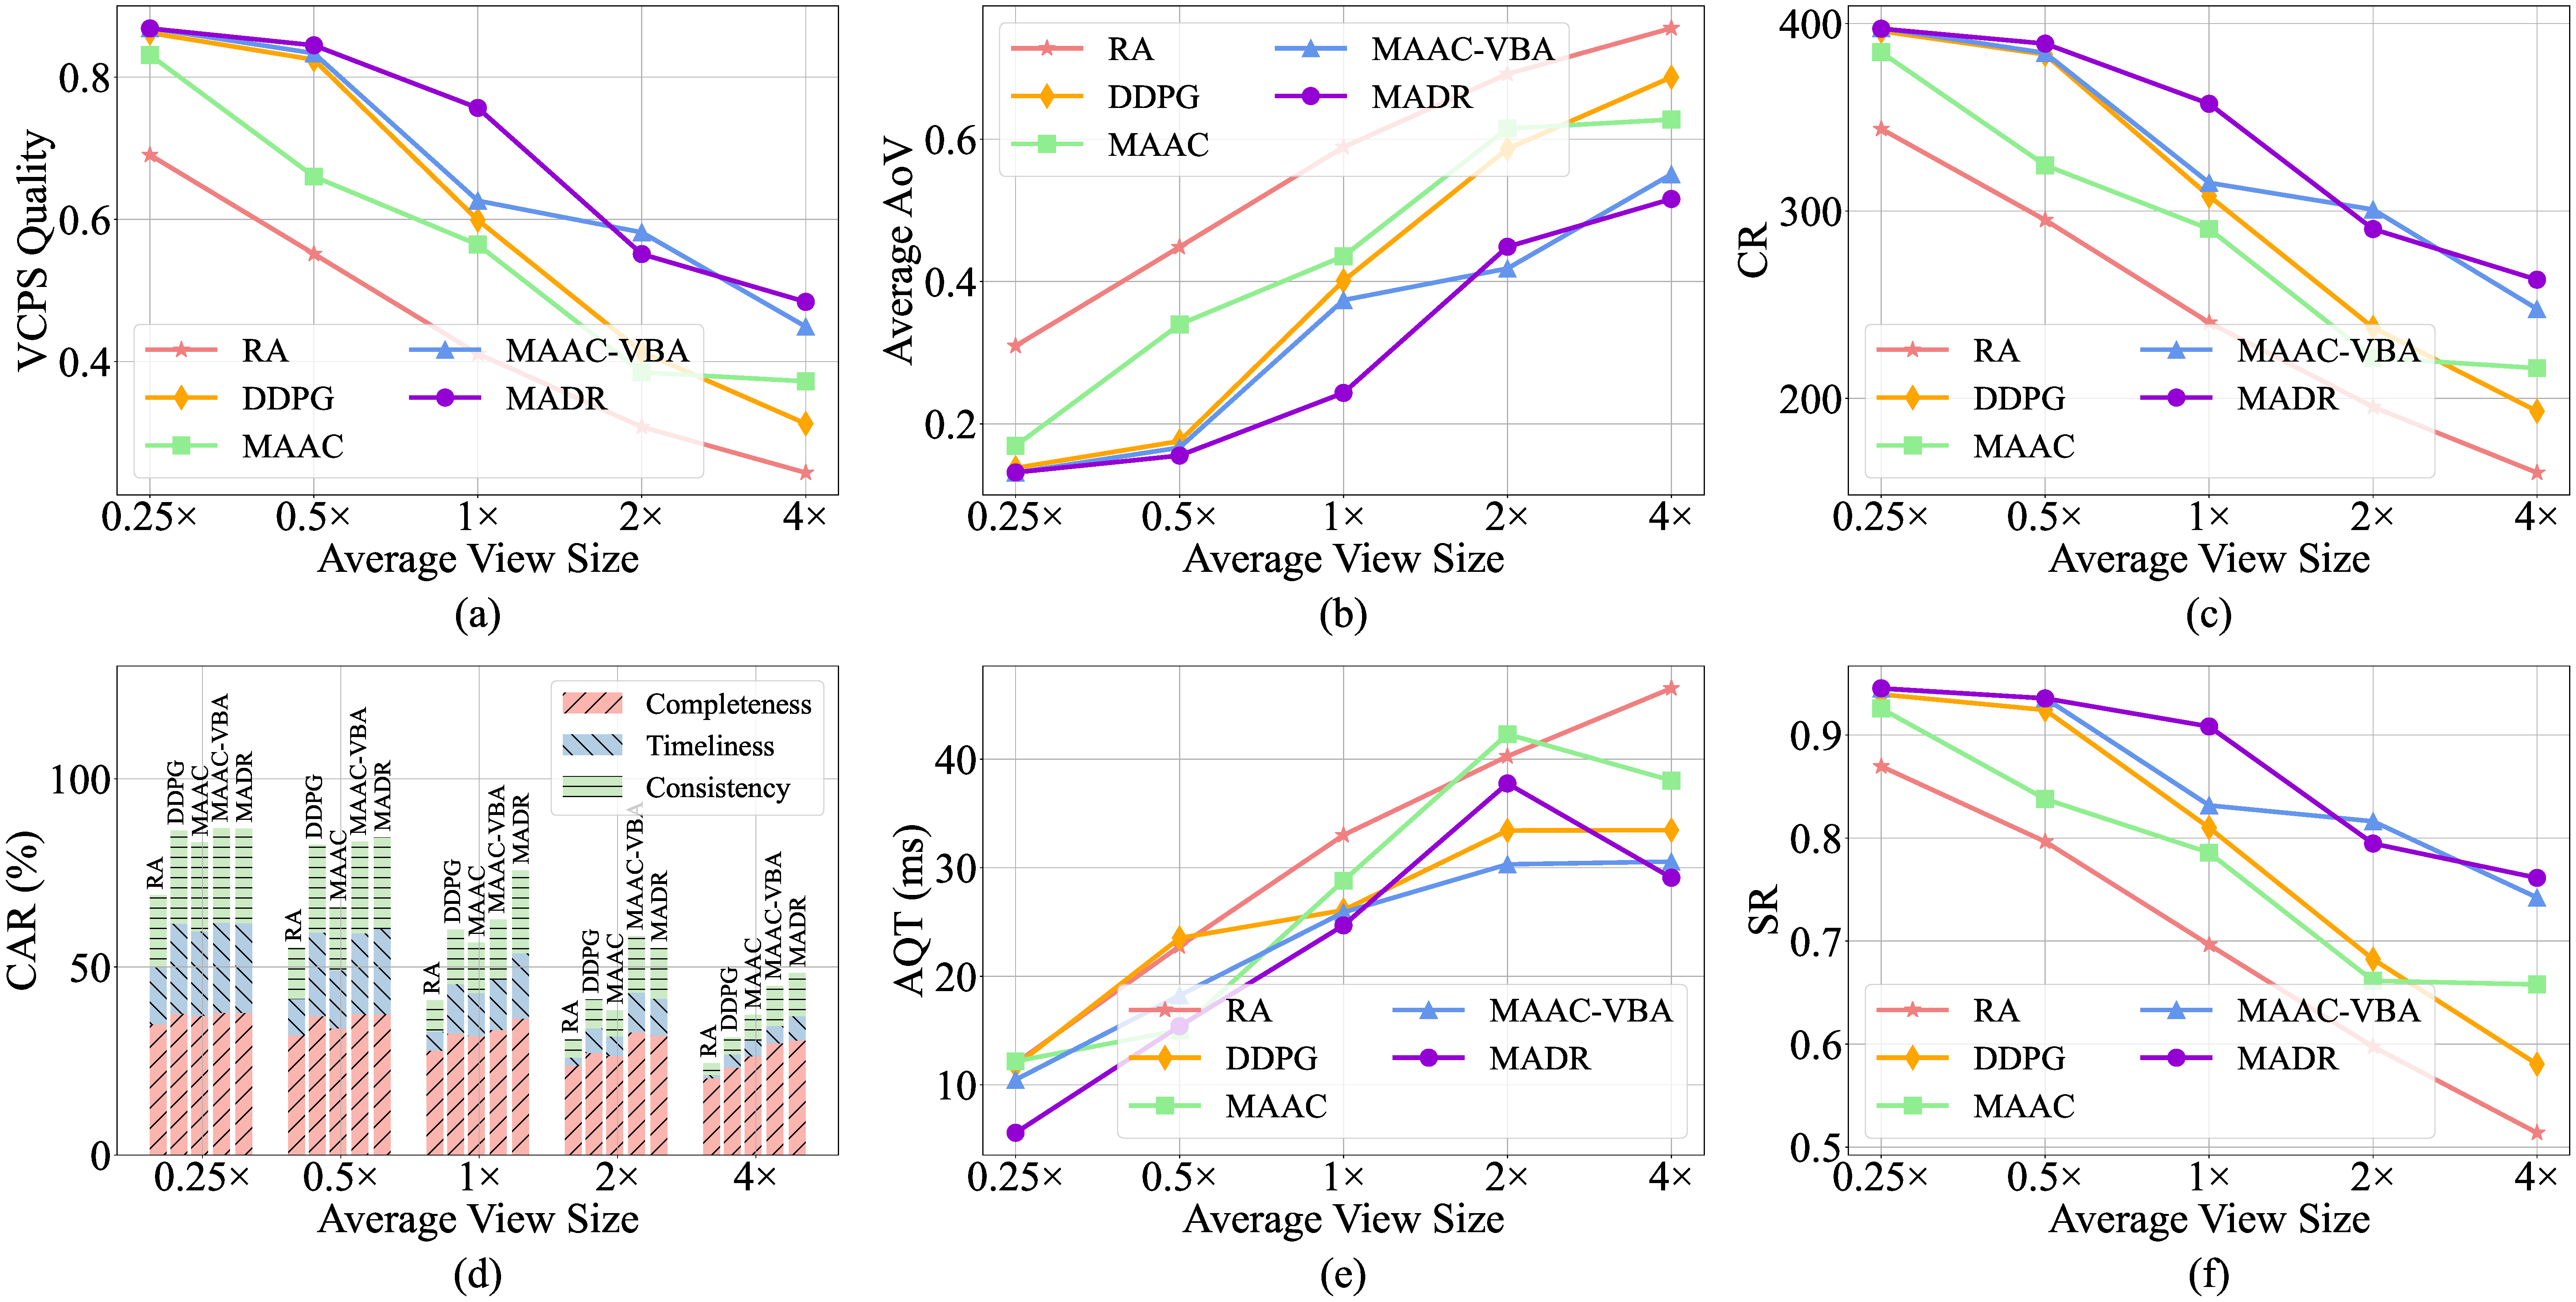
\includegraphics[width=0.9\textwidth]{fig/Fig2-9-different-view-sizes.pdf}
	\end{figure}
\end{textblock*}
\end{center}
}

\only<8-8>{
\begin{center} \englishfont \footnotesize
\begin{textblock*}{\textwidth}(-2.9cm,2cm)
{\LARGE{\color{red}\ding{216}}}
\end{textblock*}
\end{center}

\begin{center} \englishfont \footnotesize
\begin{textblock*}{\textwidth}(1cm,3.35cm)
{\LARGE{\color{red}\ding{216}}}
\end{textblock*}
\end{center}

\begin{center} \englishfont \footnotesize
\begin{textblock*}{\textwidth}(5.5cm,2cm)
{\LARGE{\color{red}\ding{216}}}
\end{textblock*}
\end{center}

\begin{center} \englishfont \footnotesize
\begin{textblock*}{\textwidth}(0.65cm,6.26cm)
{\LARGE{\color{red}\ding{216}}}
\end{textblock*}
\end{center}

\begin{center} \englishfont \footnotesize
\begin{textblock*}{\textwidth}(5.5cm,5cm)
{\LARGE{\color{red}\ding{216}}}
\end{textblock*}
\end{center}
}

\end{overlayarea}
\end{frame}
\subsection[\englishfont 2.2 面向车载信息物理融合的通信与计算资源协同优化]{2.2 面向车载信息物理融合的通信与计算资源协同优化}

\begin{frame}{研究贡献}
\newBackground
\begin{center}
\begin{textblock*}{\textwidth}(-2cm,1.8cm)
  \small \englishfont \colorbox{cqublue}{\color{white}{先进的任务调度与资源分配策略是{\color{yellow}{进}}}}
\end{textblock*}
\end{center}

\begin{center}
\begin{textblock*}{\textwidth}(-2cm,2.3cm)
  \small \englishfont \colorbox{cqublue}{\color{white}{{\color{yellow}{一步优化}}\hspace{0.2em}VCPS服务质量的{\color{yellow}{技术支撑}}}}
\end{textblock*}
\end{center}

\begin{center}
\begin{textblock*}{\textwidth}(-1.5cm,3.16cm)
\begin{minipage}[t]{0.75\textwidth}
\begin{itemize}[itemsep=0.2\baselineskip]  \englishfont
	\item[\ding{111}] {{\color{cqublue}{\textbf{问题}}}:协同资源优化 ({\color{red}{CRO}}})
	\item[\ding{111}]  {{\color{cqublue}{\textbf{算法}}}:基于博弈理论的多智能体深度强化学习 ({\color{red}{MAGT}})}
	\begin{itemize}[itemsep=0.2\baselineskip] 
	\begin{small}
		\item[\ding{226}] 问题分解
		\item[\ding{226}] 边缘节点智能体决策任务调度
		\item[\ding{226}] 凸优化最优资源分配
	\end{small}
	\end{itemize}
	\item [\ding{111}]  {{\color{cqublue}{\textbf{实验}}}:有效提高任务完成率}
	\end{itemize}
\end{minipage}
\end{textblock*}
\end{center}

\begin{center}
\begin{textblock*}{\textwidth}(-1.2cm,6.6cm)
\fbox{\begin{minipage}[t]{0.75\textwidth}\englishfont \tiny [3] \underline{\textcolor{cqublue}{XU X}}, LIU K, DAI P, et al. \textcolor{cqublue}{Joint task offloading and resource optimization in NOMA-based vehicular edge computing: A game-theoretic DRL approach}[J]. Journal of Systems Architecture (\textcolor{red}{JSA}), 2023, 134: 102780. 影响因子: 5.836(2021), 4.497(5年)  (中科院SCI 2区)
\end{minipage}}
\fbox{\begin{minipage}[t]{0.75\textwidth}\englishfont \tiny [4] \underline{\textcolor{cqublue}{许新操}}, 刘凯, 刘春晖, 等. \textcolor{cqublue}{基于势博弈的车载边缘计算信道分配方法}[J]. 电子学报, 2021. (CCF T1类中文期刊)
\end{minipage}}
\end{textblock*}
\end{center}

\begin{center}
\begin{textblock*}{\textwidth}(6.5cm,1.6cm)
\begin{figure}
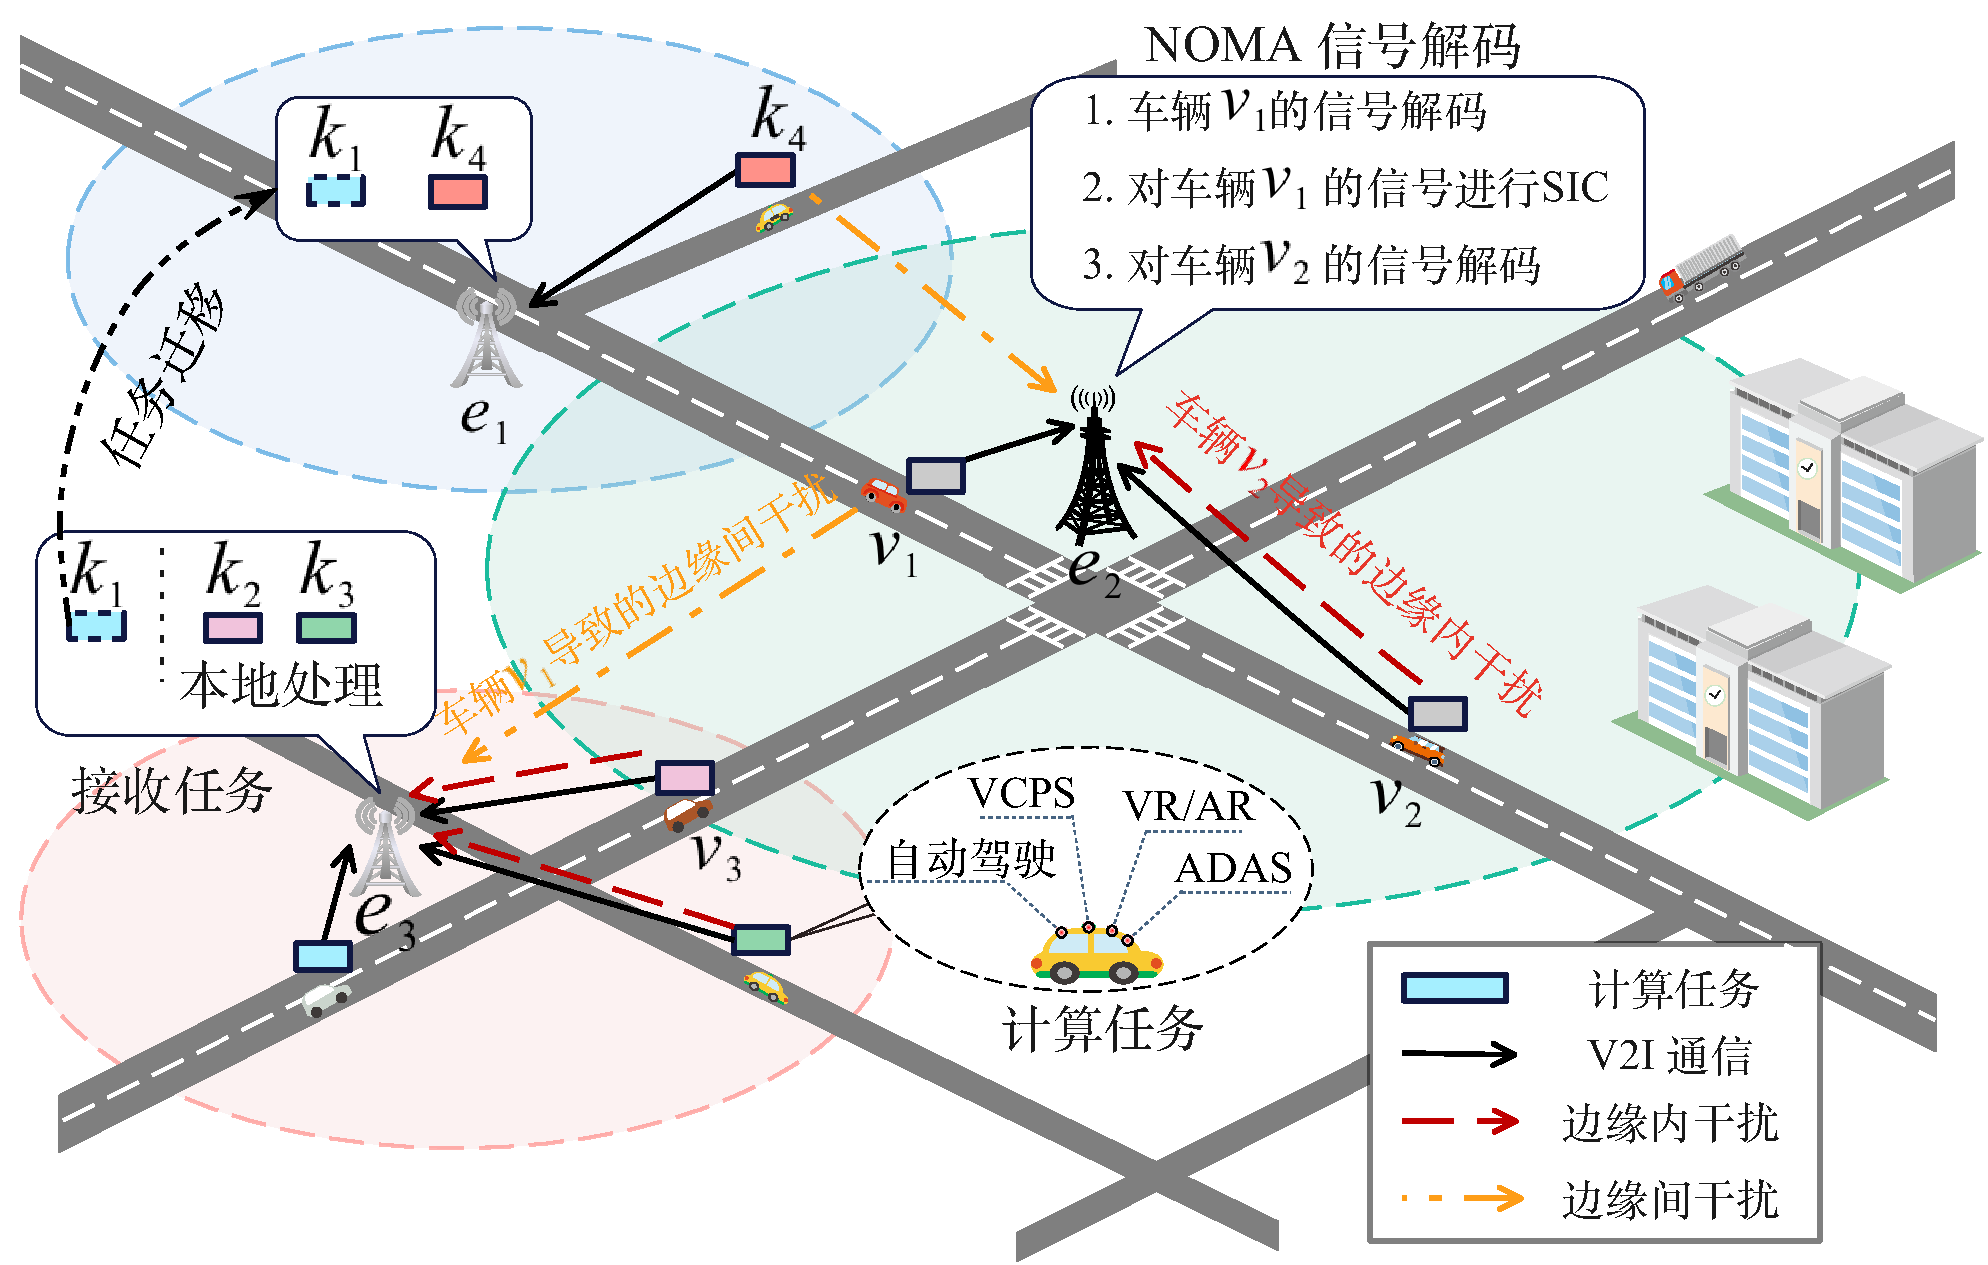
\includegraphics[width=0.3\textwidth]{fig/Fig3-1-noma-architecture.pdf}
\end{figure}
\begin{figure}
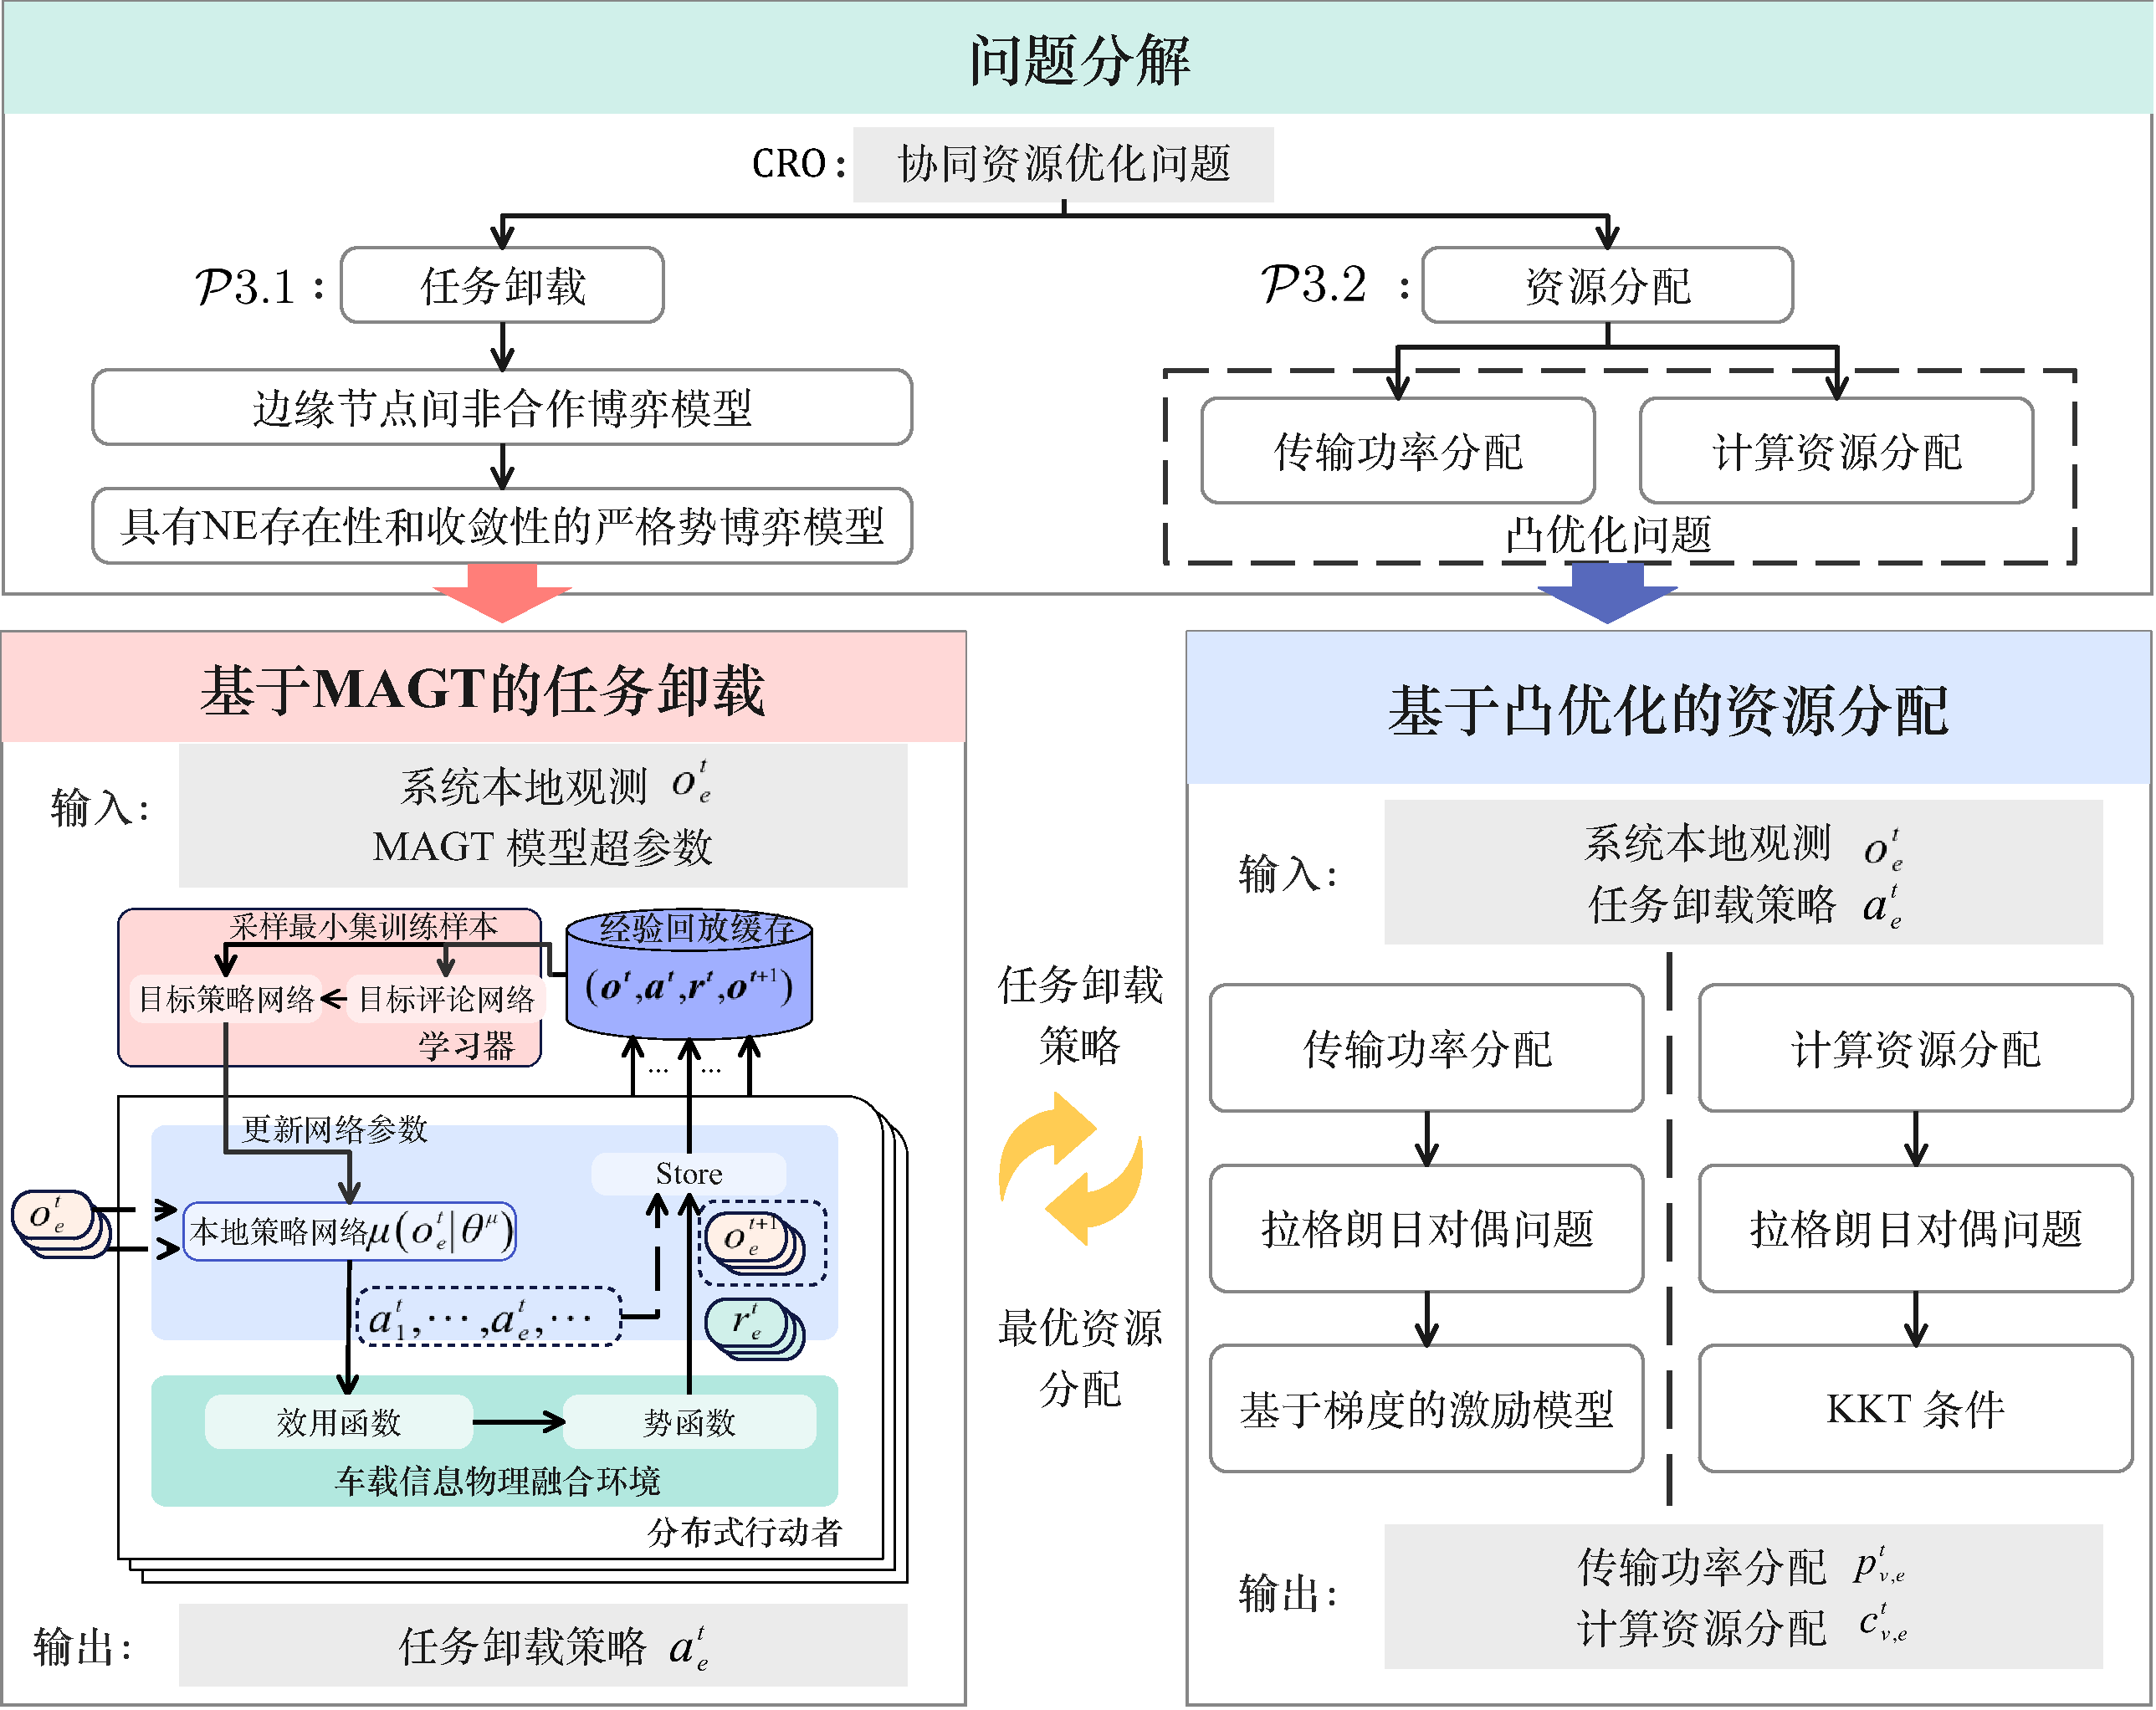
\includegraphics[width=0.3\textwidth]{fig/Fig3-3-solution-model.pdf}
\end{figure}
\end{textblock*}
\end{center}
\end{frame}

\begin{frame}
\frametitle{\englishfont \underline{问题}:协同通信与计算卸载场景}
\newBackground
\begin{center}
\begin{textblock*}{\textwidth}(5.2cm,2.4cm)
\begin{figure}
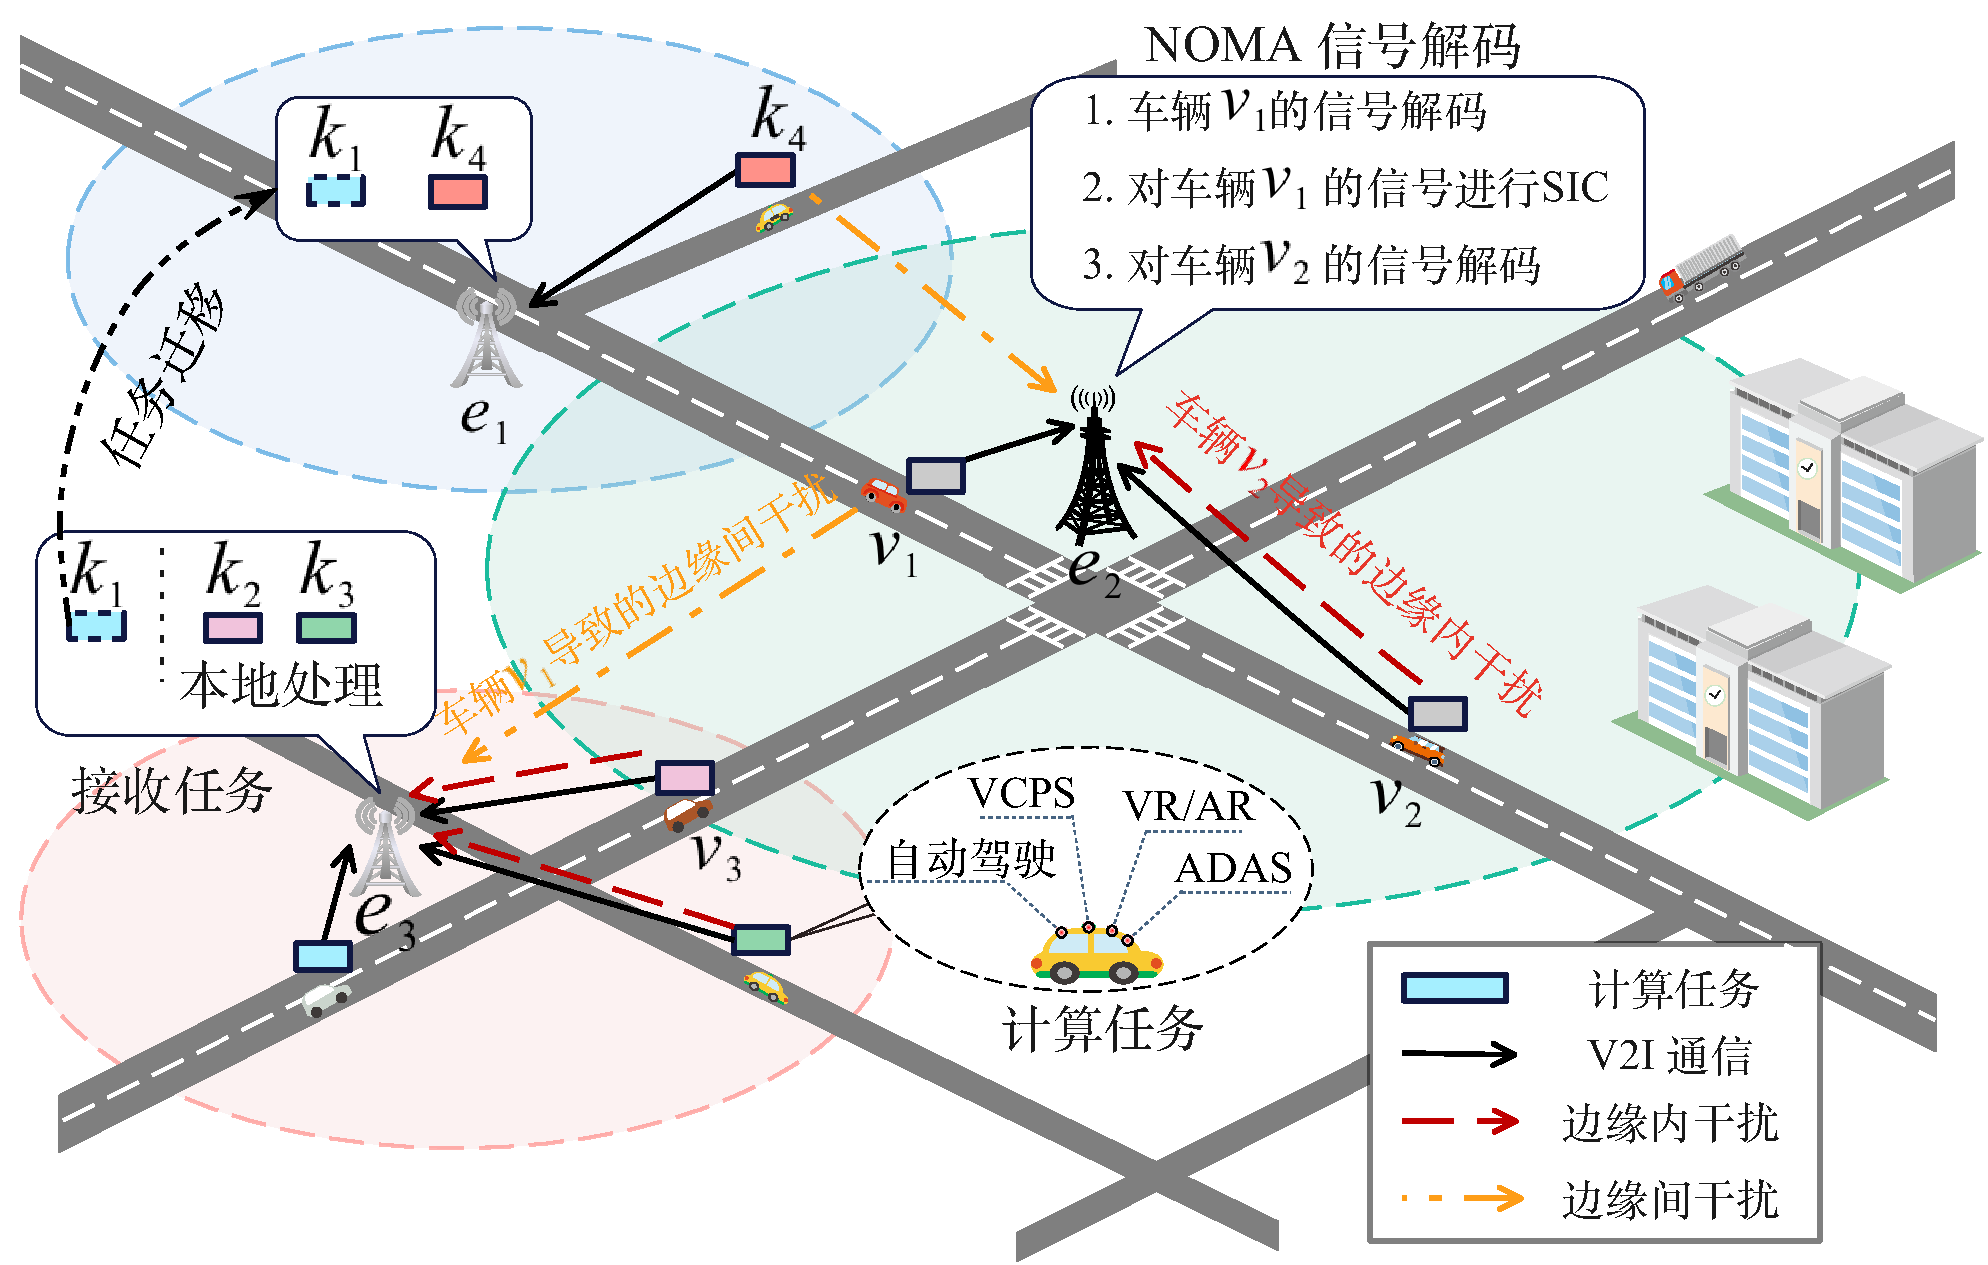
\includegraphics[width=0.55\textwidth]{fig/Fig3-1-noma-architecture.pdf}
\end{figure}
\end{textblock*}
\end{center}

\begin{center}
\begin{textblock*}{\textwidth}(0.5cm,1.8cm)
\begin{itemize}[itemsep=0.2\baselineskip] \englishfont
	\item[\ding{111}] {\color{cqublue}{工作流程}}
	\begin{itemize}[itemsep=0.2\baselineskip]
	\begin{small}
		\item[\ding{226}] \underline{计算任务产生}:车辆随机产生
		\item[\ding{226}] \underline{任务数据上传}:传输功率分配
		\begin{itemize}[itemsep=0.2\baselineskip]
		\footnotesize
			\item[\ding{61}] 车端:叠加编码
			\item[\ding{61}] 边缘端:串行干扰消除
		\end{itemize}
		\item[\ding{226}] \underline{任务本地处理/迁移}:计算资源分配
	\end{small}
	\end{itemize}
	\item[\ding{111}]  {\color{cqublue}{例子}}
	\begin{itemize}[itemsep=0.2\baselineskip]
	\begin{small}
		\item[\ding{226}] 边缘内/边缘间干扰
			\begin{itemize} \footnotesize
				\item[\ding{61}] 边缘内干扰:车辆$v_1$
				\item[\ding{61}] 边缘间干扰:车辆$v_3$
			\end{itemize}
		\item[\ding{226}] 任务负载不匀
		\begin{itemize} \footnotesize
			\item[\ding{61}] 边缘节点$e_3$ (任务$k_1$、$k_2$和$k_3$)$e_1$ (任务$k_4$)
		\end{itemize}
		\item 
	\end{small} 
	\end{itemize}
\end{itemize}
\end{textblock*}
\end{center}
\end{frame}

\begin{frame}
\frametitle{\englishfont \underline{问题}:V2I传输与任务卸载模型}
\newBackground

\begin{overlayarea}{\textwidth}{3cm}

\only<1-1>{
\begin{center}
\begin{textblock*}{1\textwidth}(-3.2cm,1.8cm)
\small	
\begin{equation}
	m_{v, e}^{t} = \frac{d_{k}}{b  \log _{2}\left(1+\mathrm{SINR}_{v, e}^t\right)} \notag
\end{equation}	
\end{textblock*}
\end{center}
}

\only<2-2>{
\begin{center}
\begin{textblock*}{1\textwidth}(-3.2cm,1.8cm)	
\small	
\begin{equation}
	m_{v, e}^{t} = \frac{d_{k}}{b  \log _{2}\left(1+{\color{red}{\mathrm{SINR}_{v, e}^t}}\right)} \notag
\end{equation}	
\end{textblock*}
\end{center}
}

\only<3->{
\begin{center}
\begin{textblock*}{1\textwidth}(-3.2cm,1.8cm)	
\small	
\begin{equation}
	m_{v, e}^{t} = \frac{d_{k}}{b  \log _{2}\left(1+\mathrm{SINR}_{v, e}^t\right)} \notag
\end{equation}	
\end{textblock*}
\end{center}
}

\only<2-2>{
\begin{center}
\begin{textblock*}{1\textwidth}(0.6cm,3.2cm)
\small
{\color{red}{$\mathrm{SINR}_{v, e}^t$}}: 信干噪比
$\mathrm{SINR}_{v, e}^t = \frac{ |h_{v, e}^t| ^{2}  p_{v, e}^{t}}{ \underbrace{\sum\limits_{\forall v^{\prime} \in \mathbf{V}_{h_{v, e}}^{t}} |h_{v^{\prime}, e}^t|^2 p_{v^{\prime}, e}^{t}}_{\text {边缘内干扰}} + \underbrace{\sum\limits_{\forall e^{\prime} \in \mathbf{E} / \{e\}} \sum\limits_{\forall v^{\prime} \in \mathbf{V}_{e^{\prime}}^{t}} |h_{v^{\prime}, e}^t|^2 p_{v^{\prime}, e^{\prime}}^{t}}_{\text {边缘间干扰}} + N_{0}}$
\end{textblock*}
\end{center}
}


\only<1-2>{
\begin{center}
\begin{textblock*}{1\textwidth}(-3.2cm,4.2cm)
\small	
\begin{equation}
	n_{v, e}^t= w_{v, e}^{t} + \sum_{\forall e^{\prime} \in \mathbf{E}} q_{v, e^{\prime}}^{t} x_{v, e^{\prime}}^t \notag
\end{equation}	
\end{textblock*}
\end{center}
}

\only<3-3>{
\begin{center}
\begin{textblock*}{1\textwidth}(-3.2cm,4.2cm)
\small	
\begin{equation}
	n_{v, e}^t= {\color{red}{w_{v, e}^{t}}} + \sum_{\forall e^{\prime} \in \mathbf{E}} q_{v, e^{\prime}}^{t} x_{v, e^{\prime}}^t \notag
\end{equation}	
\end{textblock*}
\end{center}
}

\only<3-3>{
\begin{center}
\begin{textblock*}{1\textwidth}(1.6cm,4.8cm)
\small
{\color{red}{$w_{v, e}^{t}$}}:有线传输时间
\begin{numcases}{w_{v, e}^{t} =}
0, &$k_{v}^{t} \in \mathbf{K}_{e}^{t} \bigcap \mathbf{K}_{q_e}^{t}$ \notag \\
{d_{k}  \operatorname{dis}_{e, e^{\prime}}^{t}}  \zeta  / {z},  &$k_{v}^{t} \in \mathbf{K}_{e}^{t} \bigcap \mathbf{K}_{q_{e^{\prime}}}^{t}$ \notag
\end{numcases}
\end{textblock*}
\end{center}
}

\only<4-4>{
\begin{center}
\begin{textblock*}{1\textwidth}(-3.2cm,4.2cm)
\small	
\begin{equation}
	n_{v, e}^t= w_{v, e}^{t} + \sum_{\forall e^{\prime} \in \mathbf{E}} q_{v, e^{\prime}}^{t} {\color{red}{x_{v, e^{\prime}}^t}} \notag
\end{equation}	
\end{textblock*}
\end{center}
}

\only<4-4>{
\begin{center}
\begin{textblock*}{1\textwidth}(1.6cm,4.6cm)
\small
{\color{red}{$x_{v, e^{\prime}}^t$}}:执行时间
$x_{v, e}^t = \frac{ d_{k}  c_{k}}{c_{v, e}^t}$	
\end{textblock*}
\end{center}
}

\only<5->{
\begin{center}
\begin{textblock*}{1\textwidth}(-3.2cm,4.2cm)
\small	
\begin{equation}
	n_{v, e}^t= w_{v, e}^{t} + \sum_{\forall e^{\prime} \in \mathbf{E}} q_{v, e^{\prime}}^{t} x_{v, e^{\prime}}^t \notag
\end{equation}	
\end{textblock*}
\end{center}
}
\end{overlayarea}



\begin{center}
\begin{textblock*}{1\textwidth}(1cm,1.6cm)
\begin{itemize} \englishfont 
	\item[\ding{111}]  {\color{cqublue}{任务上传时间}}
	\item
	\item 
	\item 
	\item[\ding{111}]  {\color{cqublue}{任务处理时间}}
	\item
	\item
	\item 
	\item 
	\item<5->[\ding{111}]  {\color{cqublue}{任务服务时间}}
	\item<5-> $\psi_{v, e}^{t} = m_{v, e}^{t} +  n_{v, e}^{t}$
\end{itemize}
\end{textblock*}
\end{center}

\end{frame}

\begin{frame}
\frametitle{\englishfont \underline{问题}:协作资源优化 (CRO) 问题}
\newBackground

\begin{overlayarea}{\textwidth}{3cm}
\only<1-1>{
\begin{center}
\begin{textblock*}{1\textwidth}(0.5cm,1.6cm)
\begin{align}
\operatorname{CRO}:&\max_{\mathbf{P}, \mathbf{Q}, \mathbf{C}} f_1= \sum_{\forall t \in \mathbf{T}} \sum_{ \forall e \in \mathbf{E}} \Psi_{e}^{t} \notag \\
		\text { s.t. }
    &\mathcal{C}3.1: \sum_{\forall v \in \mathbf{V}_{e}^{t}} p_{v, e}^{t} \leq p_{e}, \forall e \in \mathbf{E}, \forall t \in \mathbf{T} \notag \\
    &\mathcal{C}3.2: \sum_{\forall k_{v}^{t} \in {\mathbf{K}_{q_e}^{t} }} c_{v, e}^t \leq c_{e}, \forall e \in \mathbf{E}, \forall t \in \mathbf{T} \notag \\
   	&\mathcal{C}3.3: q_{v, e}^t \in \left \{0, 1\right \}, \forall v \in \mathbf{V}, \forall e \in \mathbf{E}, \forall t \in \mathbf{T}  \notag \\
    &\mathcal{C}3.4: \sum_{\forall e \in \mathbf{E}} q_{v, e}^t = 1, \forall v \in \mathbf{V}, \forall t \in \mathbf{T} \notag 
\end{align}
\end{textblock*}
\end{center}
}

\only<2-2>{
\begin{center}
\begin{textblock*}{1\textwidth}(0.5cm,1.6cm)
\begin{align}
\operatorname{CRO}:&\max_{\mathbf{P}, \mathbf{Q}, \mathbf{C}} f_1= \sum_{\forall t \in \mathbf{T}} \sum_{ \forall e \in \mathbf{E}} {\color{red}{\Psi_{e}^{t}}} \notag \\
		\text { s.t. }
    &\mathcal{C}3.1: \sum_{\forall v \in \mathbf{V}_{e}^{t}} p_{v, e}^{t} \leq p_{e}, \forall e \in \mathbf{E}, \forall t \in \mathbf{T} \notag \\
    &\mathcal{C}3.2: \sum_{\forall k_{v}^{t} \in {\mathbf{K}_{q_e}^{t} }} c_{v, e}^t \leq c_{e}, \forall e \in \mathbf{E}, \forall t \in \mathbf{T} \notag \\
   	&\mathcal{C}3.3: q_{v, e}^t \in \left \{0, 1\right \}, \forall v \in \mathbf{V}, \forall e \in \mathbf{E}, \forall t \in \mathbf{T}  \notag \\
    &\mathcal{C}3.4: \sum_{\forall e \in \mathbf{E}} q_{v, e}^t = 1, \forall v \in \mathbf{V}, \forall t \in \mathbf{T} \notag 
\end{align}
\end{textblock*}
\end{center}
}

\only<2-2>{
\begin{center}
\begin{textblock*}{1\textwidth}(0.5cm,7.1cm) \englishfont
{\color{red}{$\Psi_{e}^{t}$}}:服务率 $\Psi_{e}^{t} = \frac{\sum_{\forall k_{v}^{t} \in \mathbf{K}_{e}^{t}} \mathbb{I} \left\{ \psi_{v, e}^{t} \leq t_{k} \right\} }{|\mathbf{K}_{e}^{t}|}$
\end{textblock*}
\end{center}
}


\only<3-3>{
\begin{center}
\begin{textblock*}{1\textwidth}(0.5cm,1.6cm)
\begin{align}
\operatorname{CRO}:&\max_{{\color{red}{\mathbf{P}}}, \mathbf{Q}, \mathbf{C}} f_1= \sum_{\forall t \in \mathbf{T}} \sum_{ \forall e \in \mathbf{E}} \Psi_{e}^{t} \notag \\
		\text { s.t. }
    &\mathcal{C}3.1: \sum_{\forall v \in \mathbf{V}_{e}^{t}} p_{v, e}^{t} \leq p_{e}, \forall e \in \mathbf{E}, \forall t \in \mathbf{T} \notag \\
    &\mathcal{C}3.2: \sum_{\forall k_{v}^{t} \in {\mathbf{K}_{q_e}^{t} }} c_{v, e}^t \leq c_{e}, \forall e \in \mathbf{E}, \forall t \in \mathbf{T} \notag \\
   	&\mathcal{C}3.3: q_{v, e}^t \in \left \{0, 1\right \}, \forall v \in \mathbf{V}, \forall e \in \mathbf{E}, \forall t \in \mathbf{T}  \notag \\
    &\mathcal{C}3.4: \sum_{\forall e \in \mathbf{E}} q_{v, e}^t = 1, \forall v \in \mathbf{V}, \forall t \in \mathbf{T} \notag 
\end{align}
\end{textblock*}
\end{center}
}

\only<3-3>{
\begin{center}
\begin{textblock*}{1\textwidth}(0.5cm,7.1cm) \englishfont
{\color{red}{$\mathbf{P}$}}:传输功率分配 $\mathbf{P}= \left \{ p_{v, e}^{t} \mid \forall v \in \mathbf{V}_{e}^t, \forall e \in \mathbf{E}, \forall t \in \mathbf{T}\right \}$
\end{textblock*}
\end{center}
}

\only<4-4>{
\begin{center}
\begin{textblock*}{1\textwidth}(0.5cm,1.6cm)
\begin{align}
\operatorname{CRO}:&\max_{\mathbf{P}, {\color{red}{\mathbf{Q}}}, \mathbf{C}} f_1= \sum_{\forall t \in \mathbf{T}} \sum_{ \forall e \in \mathbf{E}} \Psi_{e}^{t} \notag \\
		\text { s.t. }
    &\mathcal{C}3.1: \sum_{\forall v \in \mathbf{V}_{e}^{t}} p_{v, e}^{t} \leq p_{e}, \forall e \in \mathbf{E}, \forall t \in \mathbf{T} \notag \\
    &\mathcal{C}3.2: \sum_{\forall k_{v}^{t} \in {\mathbf{K}_{q_e}^{t} }} c_{v, e}^t \leq c_{e}, \forall e \in \mathbf{E}, \forall t \in \mathbf{T} \notag \\
   	&\mathcal{C}3.3: q_{v, e}^t \in \left \{0, 1\right \}, \forall v \in \mathbf{V}, \forall e \in \mathbf{E}, \forall t \in \mathbf{T}  \notag \\
    &\mathcal{C}3.4: \sum_{\forall e \in \mathbf{E}} q_{v, e}^t = 1, \forall v \in \mathbf{V}, \forall t \in \mathbf{T} \notag 
\end{align}
\end{textblock*}
\end{center}
}

\only<4-4>{
\begin{center}
\begin{textblock*}{1\textwidth}(0.5cm,7.1cm) \englishfont
{\color{red}{$\mathbf{Q}$}}:任务卸载决策 $\mathbf{Q}= \left \{ q_{v, e}^t \mid \forall v \in \mathbf{V}, \forall e \in \mathbf{E}, \forall t \in \mathbf{T} \right \}$
\end{textblock*}
\end{center}
}

\only<5-5>{
\begin{center}
\begin{textblock*}{1\textwidth}(0.5cm,1.6cm)
\begin{align}
\operatorname{CRO}:&\max_{\mathbf{P}, \mathbf{Q}, {\color{red}{\mathbf{C}}}} f_1= \sum_{\forall t \in \mathbf{T}} \sum_{ \forall e \in \mathbf{E}} \Psi_{e}^{t} \notag \\
		\text { s.t. }
    &\mathcal{C}3.1: \sum_{\forall v \in \mathbf{V}_{e}^{t}} p_{v, e}^{t} \leq p_{e}, \forall e \in \mathbf{E}, \forall t \in \mathbf{T} \notag \\
    &\mathcal{C}3.2: \sum_{\forall k_{v}^{t} \in {\mathbf{K}_{q_e}^{t} }} c_{v, e}^t \leq c_{e}, \forall e \in \mathbf{E}, \forall t \in \mathbf{T} \notag \\
   	&\mathcal{C}3.3: q_{v, e}^t \in \left \{0, 1\right \}, \forall v \in \mathbf{V}, \forall e \in \mathbf{E}, \forall t \in \mathbf{T}  \notag \\
    &\mathcal{C}3.4: \sum_{\forall e \in \mathbf{E}} q_{v, e}^t = 1, \forall v \in \mathbf{V}, \forall t \in \mathbf{T} \notag 
\end{align}
\end{textblock*}
\end{center}
}

\only<5-5>{
\begin{center}
\begin{textblock*}{1\textwidth}(0.5cm,7.1cm) \englishfont
{\color{red}{$\mathbf{C}$}}:计算资源分配 $\mathbf{C}= \left \{ c_{v, e}^t \mid \forall v \in \mathbf{V}, \forall e \in \mathbf{E}, \forall t \in \mathbf{T} \right \}$
\end{textblock*}
\end{center}
}

\only<6-6>{
\begin{center}
\begin{textblock*}{1\textwidth}(0.5cm,1.6cm)
\begin{align}
\operatorname{CRO}:&\max_{\mathbf{P}, \mathbf{Q}, \mathbf{C}} f_1= \sum_{\forall t \in \mathbf{T}} \sum_{ \forall e \in \mathbf{E}} \Psi_{e}^{t} \notag \\
		\text { s.t. }
    &{\color{red}{\mathcal{C}3.1}}: \sum_{\forall v \in \mathbf{V}_{e}^{t}} p_{v, e}^{t} \leq p_{e}, \forall e \in \mathbf{E}, \forall t \in \mathbf{T} \notag \\
    &\mathcal{C}3.2: \sum_{\forall k_{v}^{t} \in {\mathbf{K}_{q_e}^{t} }} c_{v, e}^t \leq c_{e}, \forall e \in \mathbf{E}, \forall t \in \mathbf{T} \notag \\
   	&\mathcal{C}3.3: q_{v, e}^t \in \left \{0, 1\right \}, \forall v \in \mathbf{V}, \forall e \in \mathbf{E}, \forall t \in \mathbf{T}  \notag \\
    &\mathcal{C}3.4: \sum_{\forall e \in \mathbf{E}} q_{v, e}^t = 1, \forall v \in \mathbf{V}, \forall t \in \mathbf{T} \notag 
\end{align}
\end{textblock*}
\end{center}
}

\only<6-6>{
\begin{center}
\begin{textblock*}{1\textwidth}(0.5cm,7.1cm) \englishfont
{\color{red}{$\mathcal{C}3.1$}}:边缘节点分配的总传输功率不能超过V2I通信的最大功率
\end{textblock*}
\end{center}
}

\only<7-7>{
\begin{center}
\begin{textblock*}{1\textwidth}(0.5cm,1.6cm)
\begin{align}
\operatorname{CRO}:&\max_{\mathbf{P}, \mathbf{Q}, \mathbf{C}} f_1= \sum_{\forall t \in \mathbf{T}} \sum_{ \forall e \in \mathbf{E}} \Psi_{e}^{t} \notag \\
		\text { s.t. }
    &\mathcal{C}3.1: \sum_{\forall v \in \mathbf{V}_{e}^{t}} p_{v, e}^{t} \leq p_{e}, \forall e \in \mathbf{E}, \forall t \in \mathbf{T} \notag \\
    &{\color{red}{\mathcal{C}3.2}}: \sum_{\forall k_{v}^{t} \in {\mathbf{K}_{q_e}^{t} }} c_{v, e}^t \leq c_{e}, \forall e \in \mathbf{E}, \forall t \in \mathbf{T} \notag \\
   	&\mathcal{C}3.3: q_{v, e}^t \in \left \{0, 1\right \}, \forall v \in \mathbf{V}, \forall e \in \mathbf{E}, \forall t \in \mathbf{T}  \notag \\
    &\mathcal{C}3.4: \sum_{\forall e \in \mathbf{E}} q_{v, e}^t = 1, \forall v \in \mathbf{V}, \forall t \in \mathbf{T} \notag 
\end{align}
\end{textblock*}
\end{center}
}

\only<7-7>{
\begin{center}
\begin{textblock*}{1\textwidth}(0.5cm,7.1cm) \englishfont
{\color{red}{$\mathcal{C}2.2$}}:分配的总体计算资源不能超过边缘节点的计算能力
\end{textblock*}
\end{center}
}

\only<8-8>{
\begin{center}
\begin{textblock*}{1\textwidth}(0.5cm,1.6cm)
\begin{align}
\operatorname{CRO}:&\max_{\mathbf{P}, \mathbf{Q}, \mathbf{C}} f_1= \sum_{\forall t \in \mathbf{T}} \sum_{ \forall e \in \mathbf{E}} \Psi_{e}^{t} \notag \\
		\text { s.t. }
    &\mathcal{C}3.1: \sum_{\forall v \in \mathbf{V}_{e}^{t}} p_{v, e}^{t} \leq p_{e}, \forall e \in \mathbf{E}, \forall t \in \mathbf{T} \notag \\
    &\mathcal{C}3.2: \sum_{\forall k_{v}^{t} \in {\mathbf{K}_{q_e}^{t} }} c_{v, e}^t \leq c_{e}, \forall e \in \mathbf{E}, \forall t \in \mathbf{T} \notag \\
   	&{\color{red}{\mathcal{C}3.3}}: q_{v, e}^t \in \left \{0, 1\right \}, \forall v \in \mathbf{V}, \forall e \in \mathbf{E}, \forall t \in \mathbf{T}  \notag \\
    &\mathcal{C}3.4: \sum_{\forall e \in \mathbf{E}} q_{v, e}^t = 1, \forall v \in \mathbf{V}, \forall t \in \mathbf{T} \notag 
\end{align}
\end{textblock*}
\end{center}
}

\only<8-8>{
\begin{center}
\begin{textblock*}{1\textwidth}(0.5cm,7.1cm) \englishfont
{\color{red}{$\mathcal{C}3.3$}}:任务卸载决策是 0-1 变量
\end{textblock*}
\end{center}
}

\only<9-9>{
\begin{center}
\begin{textblock*}{1\textwidth}(0.5cm,1.6cm)
\begin{align}
\operatorname{CRO}:&\max_{\mathbf{P}, \mathbf{Q}, \mathbf{C}} f_1= \sum_{\forall t \in \mathbf{T}} \sum_{ \forall e \in \mathbf{E}} \Psi_{e}^{t} \notag \\
		\text { s.t. }
    &\mathcal{C}3.1: \sum_{\forall v \in \mathbf{V}_{e}^{t}} p_{v, e}^{t} \leq p_{e}, \forall e \in \mathbf{E}, \forall t \in \mathbf{T} \notag \\
    &\mathcal{C}3.2: \sum_{\forall k_{v}^{t} \in {\mathbf{K}_{q_e}^{t} }} c_{v, e}^t \leq c_{e}, \forall e \in \mathbf{E}, \forall t \in \mathbf{T} \notag \\
   	&\mathcal{C}3.3: q_{v, e}^t \in \left \{0, 1\right \}, \forall v \in \mathbf{V}, \forall e \in \mathbf{E}, \forall t \in \mathbf{T}  \notag \\
    &{\color{red}{\mathcal{C}3.4}}: \sum_{\forall e \in \mathbf{E}} q_{v, e}^t = 1, \forall v \in \mathbf{V}, \forall t \in \mathbf{T} \notag 
\end{align}
\end{textblock*}
\end{center}
}

\only<9-9>{
\begin{center}
\begin{textblock*}{1\textwidth}(0.5cm,7.1cm) \englishfont
{\color{red}{$\mathcal{C}3.4$}}:每个任务只能卸载到一个边缘节点
\end{textblock*}
\end{center}
}


\end{overlayarea}
\end{frame}

\begin{frame}
\frametitle{\englishfont \underline{算法}:问题分解}
\newBackground
\begin{center}
\begin{textblock*}{\textwidth}(5.7cm,2.3cm)
\begin{figure}
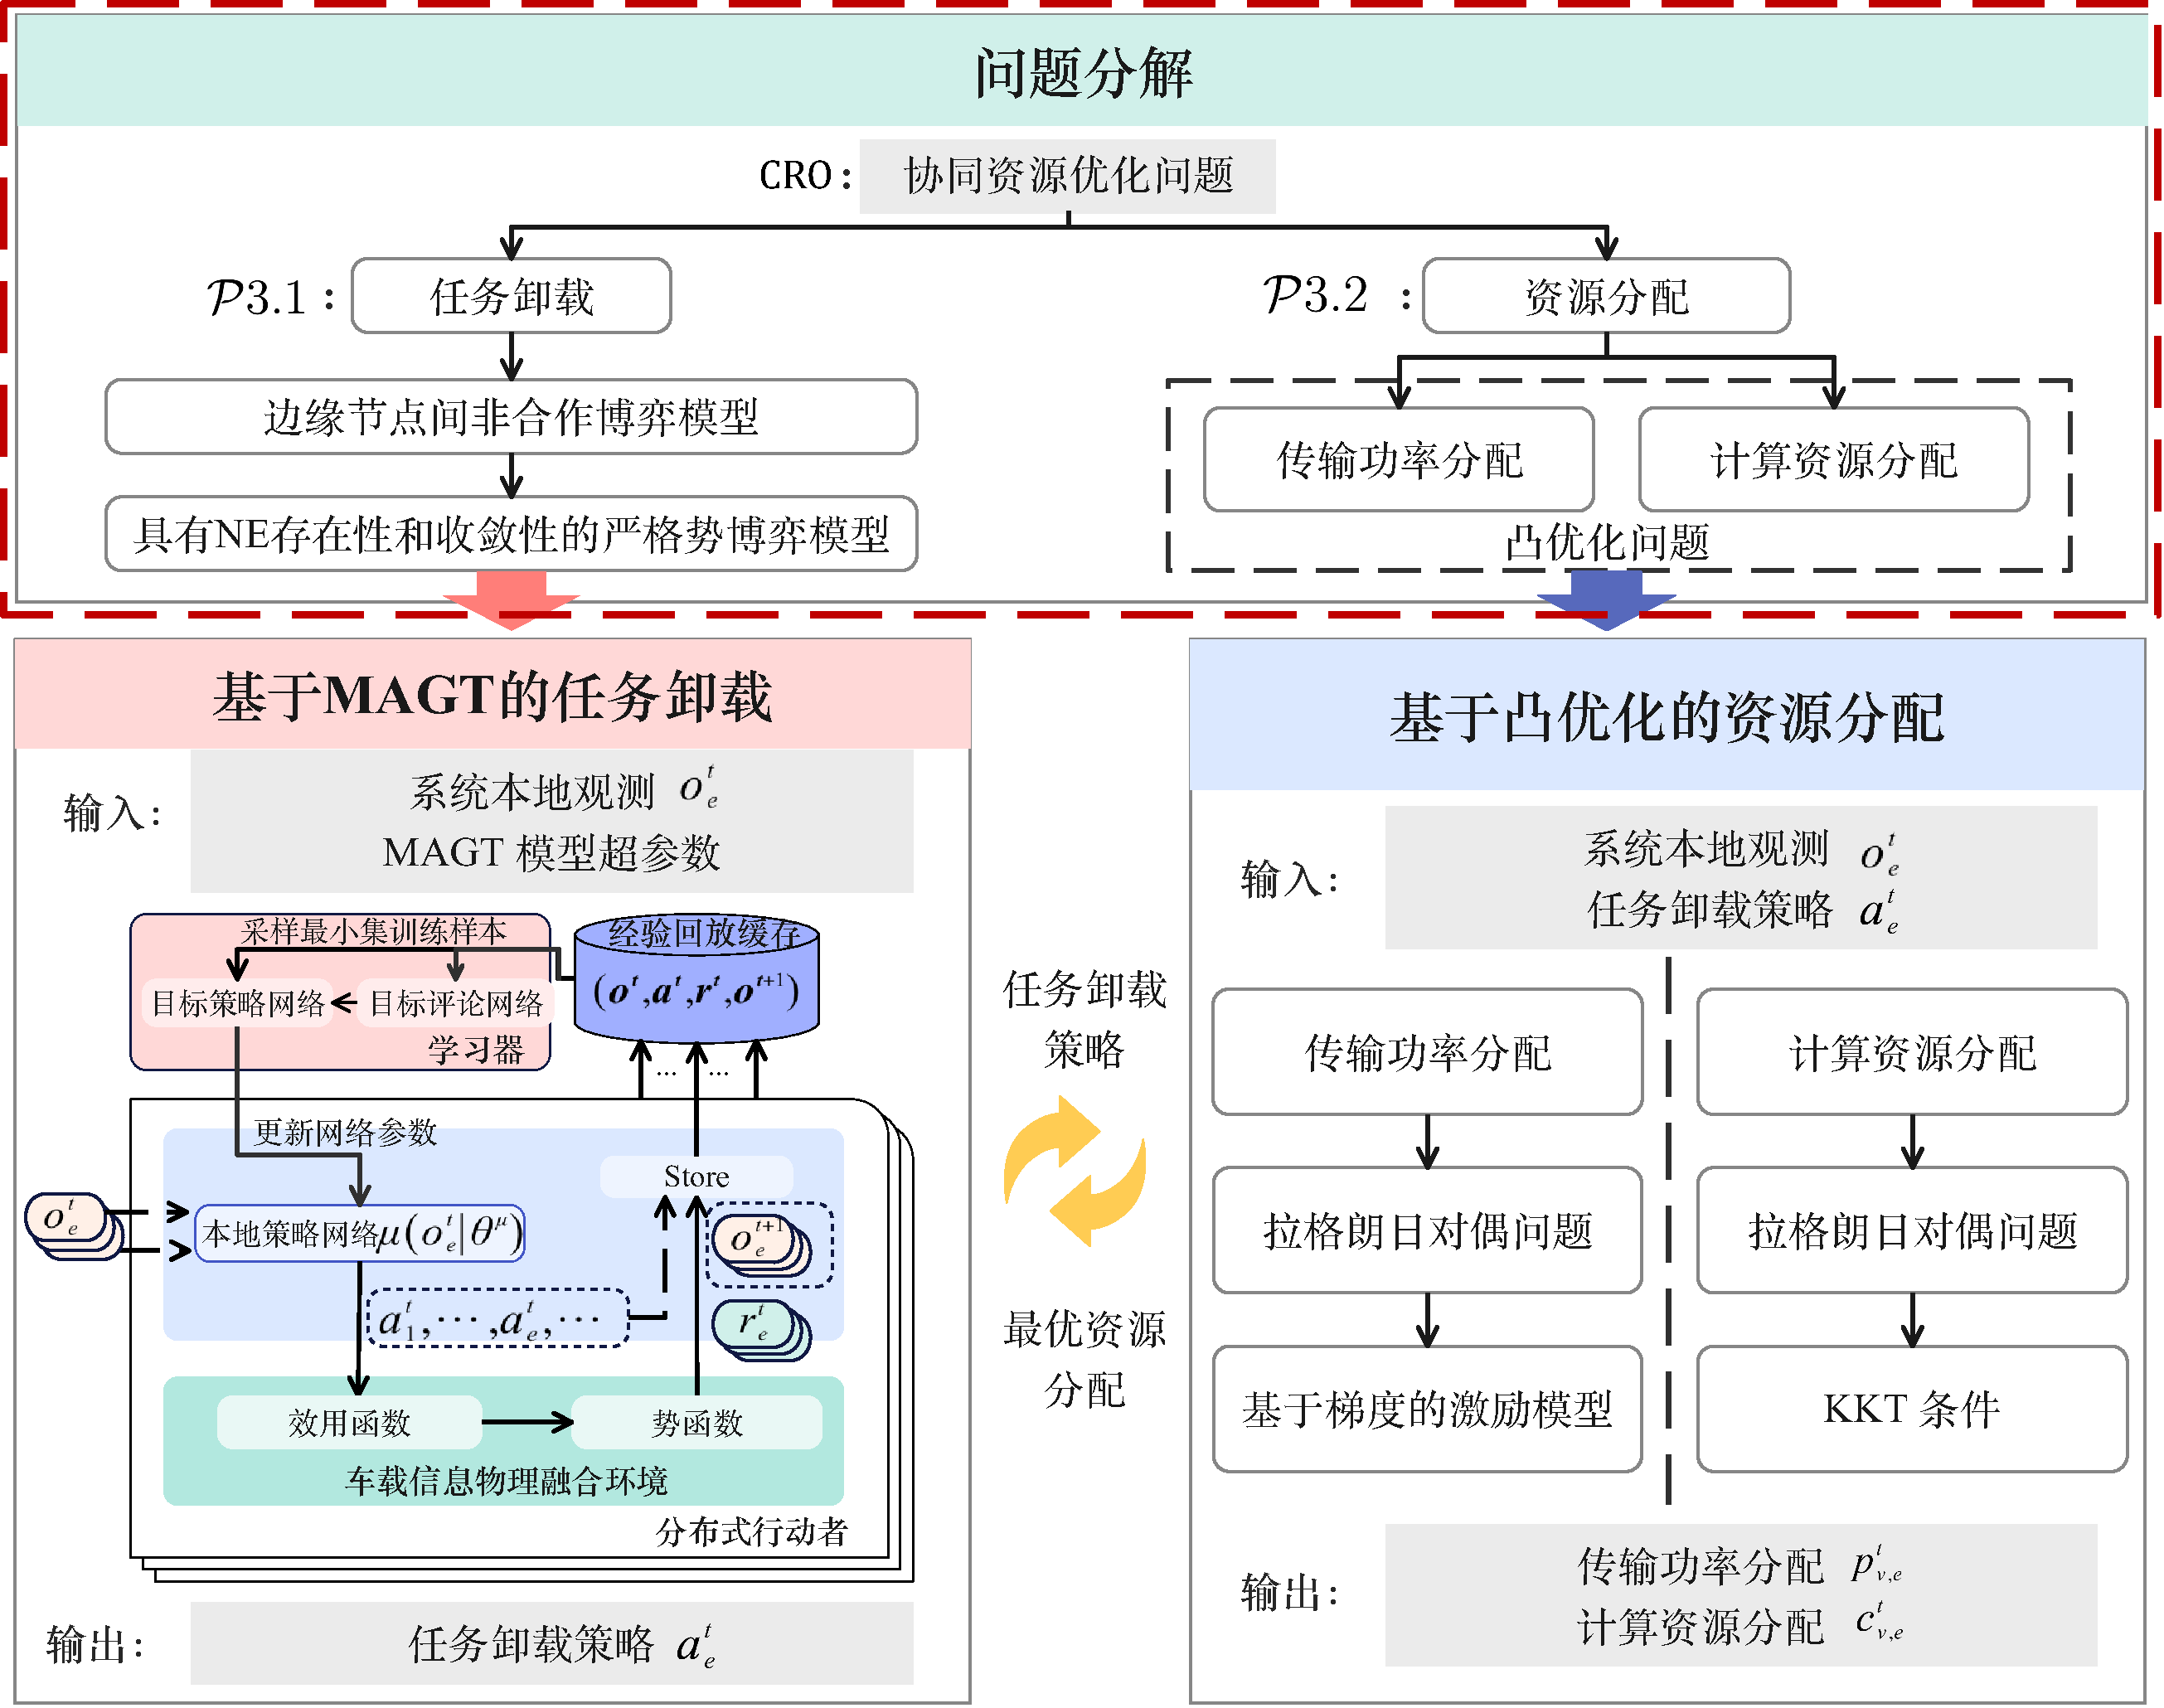
\includegraphics[width=0.45\textwidth]{fig/Fig3-3-solution-model1.pdf}
\end{figure}
\end{textblock*}
\end{center}

\begin{center}
\begin{textblock*}{0.75\textwidth}(0.5cm,2cm)
\begin{itemize}[itemsep=0.2\baselineskip] \englishfont 
	\item[\ding{111}] {\color{cqublue}{任务卸载问题}}
	\begin{itemize}[itemsep=0.2\baselineskip]
	\begin{small}
		\item[\ding{226}] 边缘节点非合作博弈{\small{$\mathcal{G} = \left\{\mathbf{E}, \mathbb{S}, \left\{{U}_{e}\right\}_{\forall e \in \mathbf{E}} \right\}$}}
		\item[\ding{226}] 效用函数{\small{${U}_{e}\left(\mathcal{S}\right) = \sum_{\forall e \in \mathbf{E}} \Psi_{e}^{t}$}}
		\item[\ding{226}] 势函数{\small{${F}_{e}\left(\mathcal{S}\right) = {U}_{e}\left(\mathcal{S}_{e}, \mathcal{S}_{-e}\right) - {U}_{e}\left(-\mathcal{S}_{e}, \mathcal{S}_{-e}\right)$}}
		\item[\ding{226}] 具有NE存在和收敛性的严格势博弈 (EPG)
	\end{small}
	\end{itemize}
	\item[\ding{111}]  {\color{cqublue}{资源分配问题}}
	\begin{itemize}[itemsep=0.2\baselineskip]
	\begin{small}
		\item[\ding{226}] 传输功率分配\\{\small{$ \min_{\mathbf{P}^{t}} \sum_{ \forall e \in \mathbf{E}} \sum_{\forall k_{v}^{t} \in \mathbf{K}_{e}^{t}}  \frac{d_{k}}{b  \log _{2}\left(1+\mathrm{SINR}_{v, e}^t\right)}$}}
		\item[\ding{226}] 计算资源分配\\{\small{$ \min_{\mathbf{C}^{t}} \sum_{ \forall e \in \mathbf{E}} \sum_{\forall k_{v}^{t} \in \mathbf{K}_{e}^{t}} ( w_{v, e}^{t} + \sum_{\forall e^{\prime} \in \mathbf{E}} q_{v, e^{\prime}}^{t} x_{v, e^{\prime}}^t)$}}
	\end{small}
	\end{itemize}
\end{itemize}
\end{textblock*}
\end{center}
\end{frame}

\begin{frame}
\frametitle{\englishfont \underline{算法}:基于MAGT的任务卸载}
\newBackground
\begin{center}
\begin{textblock*}{\textwidth}(5.7cm,2.3cm)
\begin{figure}
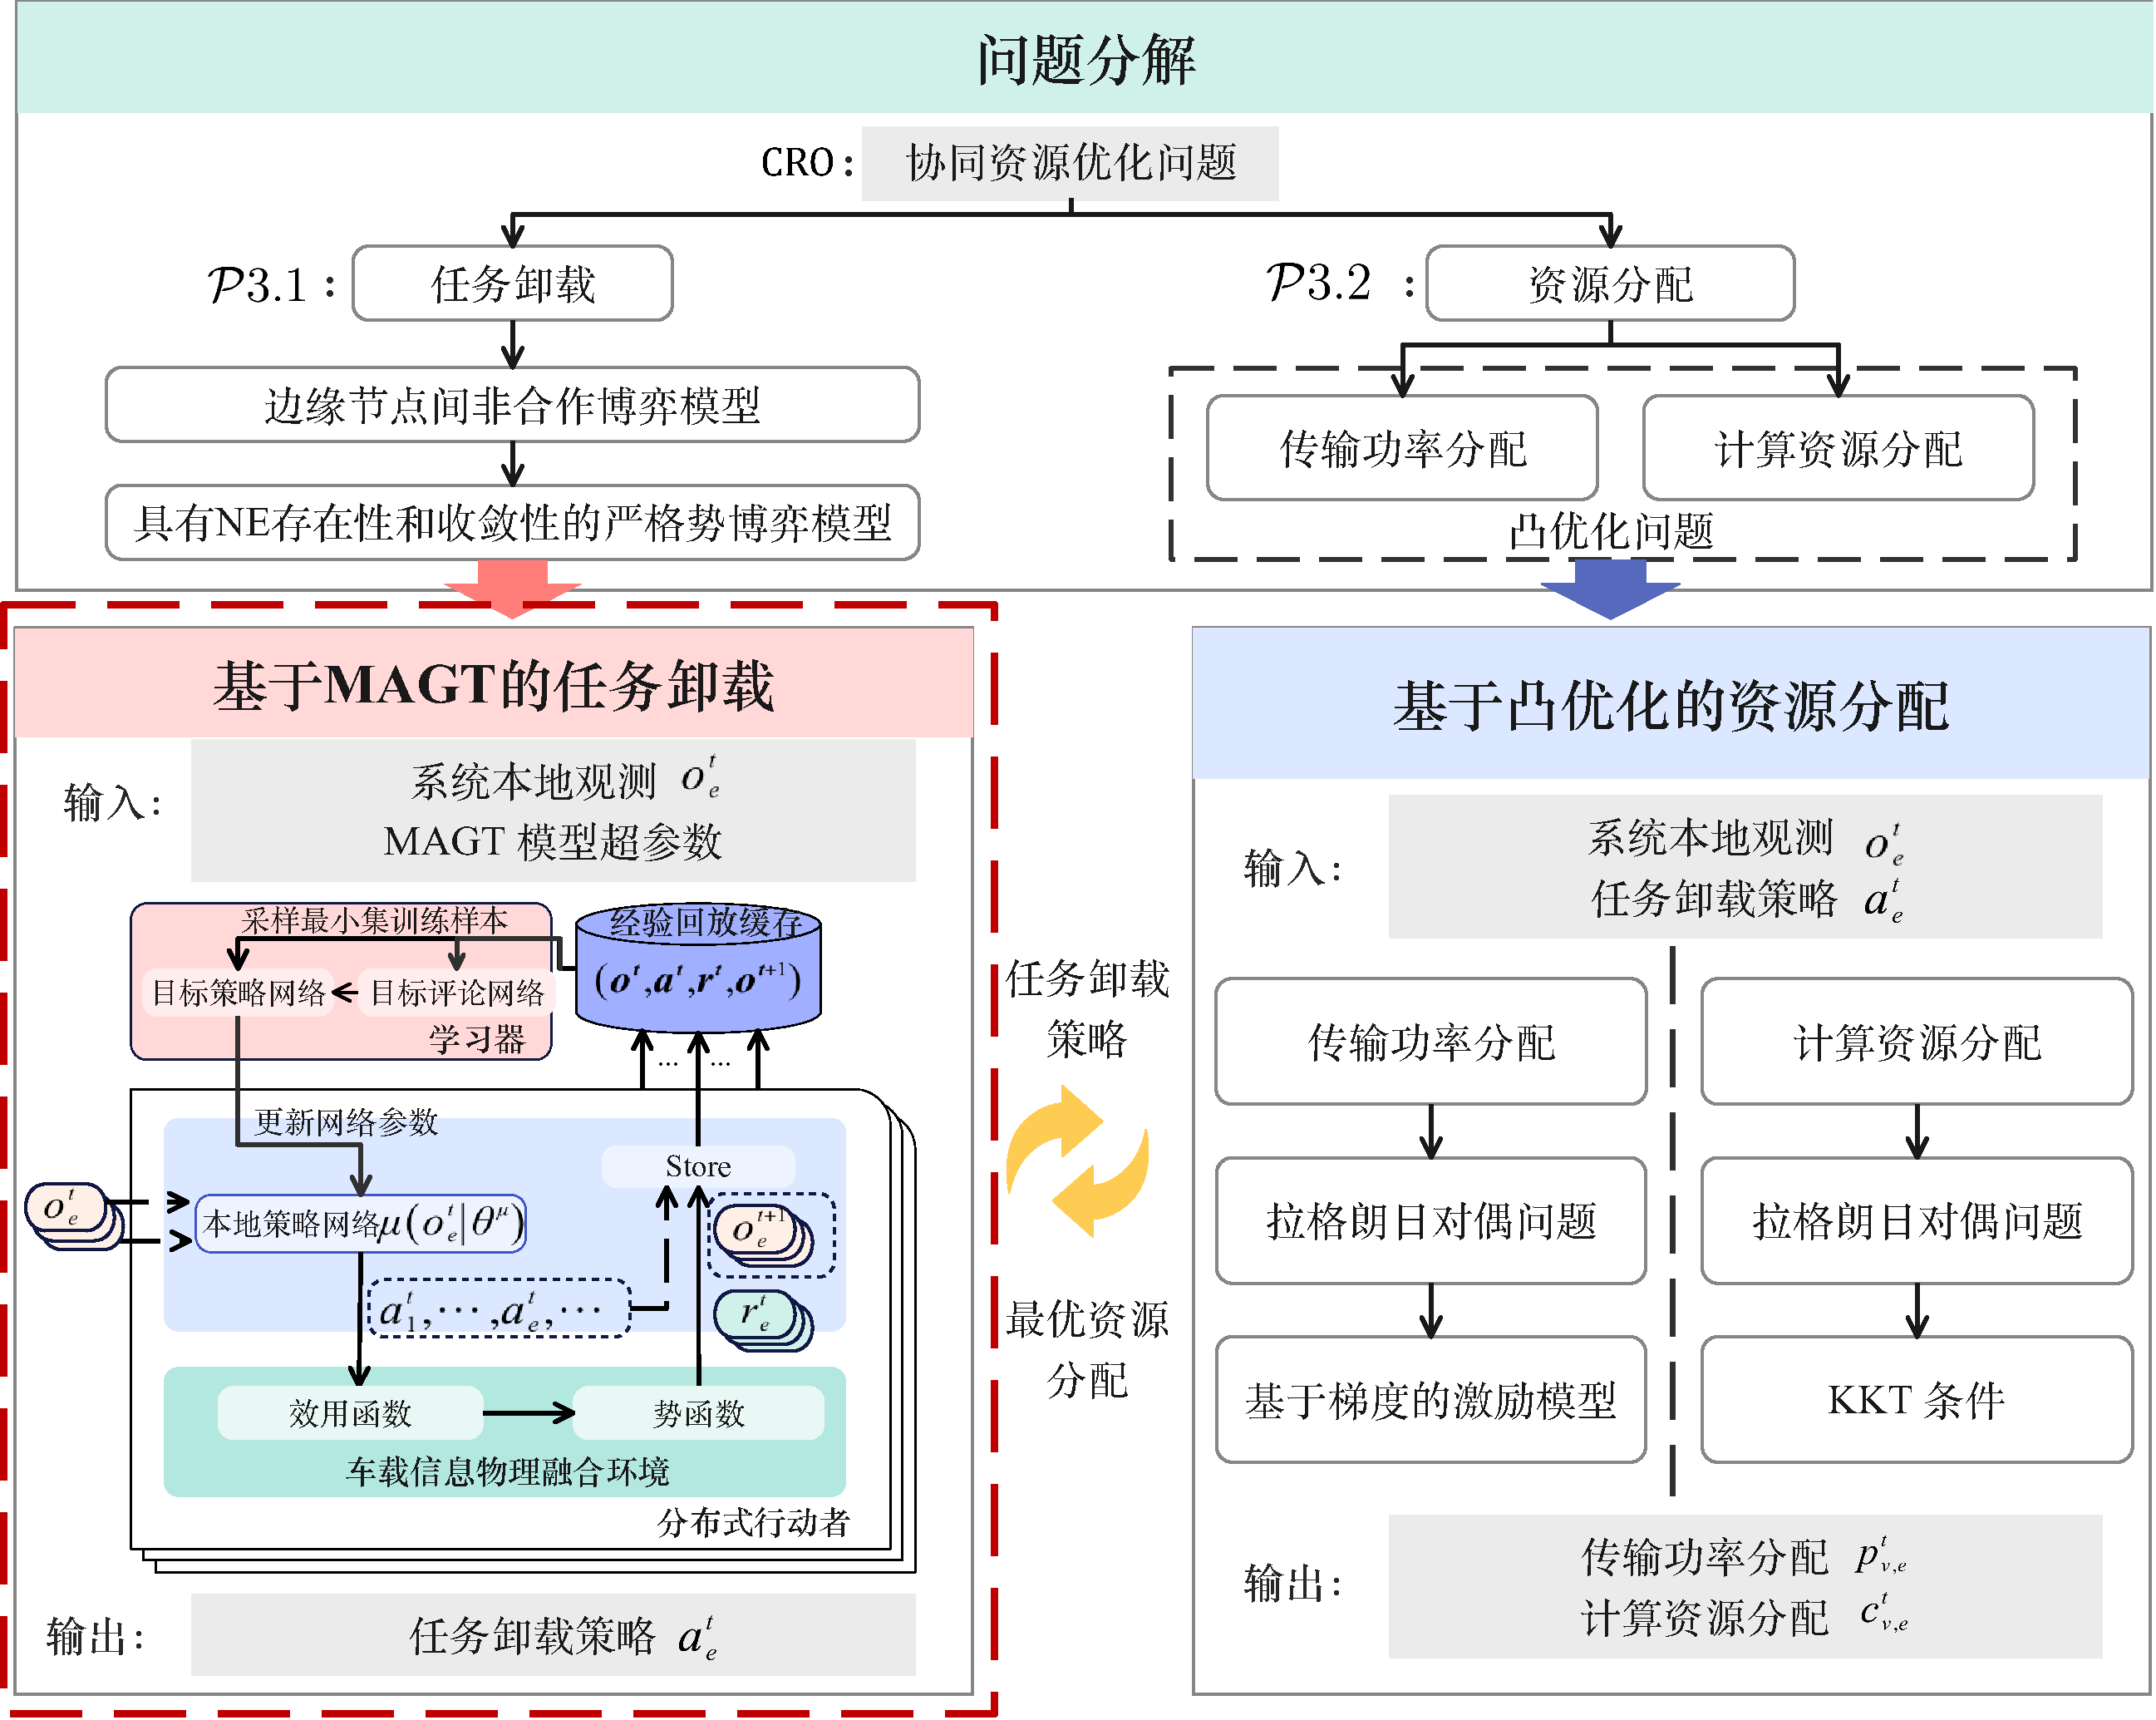
\includegraphics[width=0.45\textwidth]{fig/Fig3-3-solution-model2.pdf}
\end{figure}
\end{textblock*}
\end{center}

\begin{center}
\begin{textblock*}{0.6\textwidth}(0.5cm,2cm)
\begin{itemize} \englishfont
	\item[\ding{111}] {\color{cqublue}{系统状态}}
	\item 边缘节点观测
	\item $\boldsymbol{o}_{e}^{t}=\left\{e, t, \mathbf{Dis}_{\mathbf{V}_{e}^{t}}, \mathbf{D}_{\mathbf{K}_{e}^{t}}, \mathbf{C}_{\mathbf{K}_{e}^{t}}, \mathbf{T}_{\mathbf{K}_{v}^{t}}\right\}$
	\item[\ding{111}] {\color{cqublue}{动作空间}}
	\item 车辆请求任务的卸载决策
	\item $\boldsymbol{a}_{e}^{t} = \left\{ q_{v, e^{\prime}}^t \mid \forall e^{\prime} \in \mathbf{E}, \forall v \in \mathbf{V}_{e}^{t} \right\}$
	\item[\ding{111}] {\color{cqublue}{奖励函数}}
	\item 博弈中效用函数\ding{221}系统奖励函数
	\item 博弈中势函数\ding{221}边缘节点奖励函数
\end{itemize}
\end{textblock*}
\end{center}

\end{frame}

\begin{frame}
\frametitle{\englishfont \underline{算法}:基于凸优化的资源分配}
\newBackground
\begin{center}
\begin{textblock*}{\textwidth}(5.7cm,2.3cm)
\begin{figure}
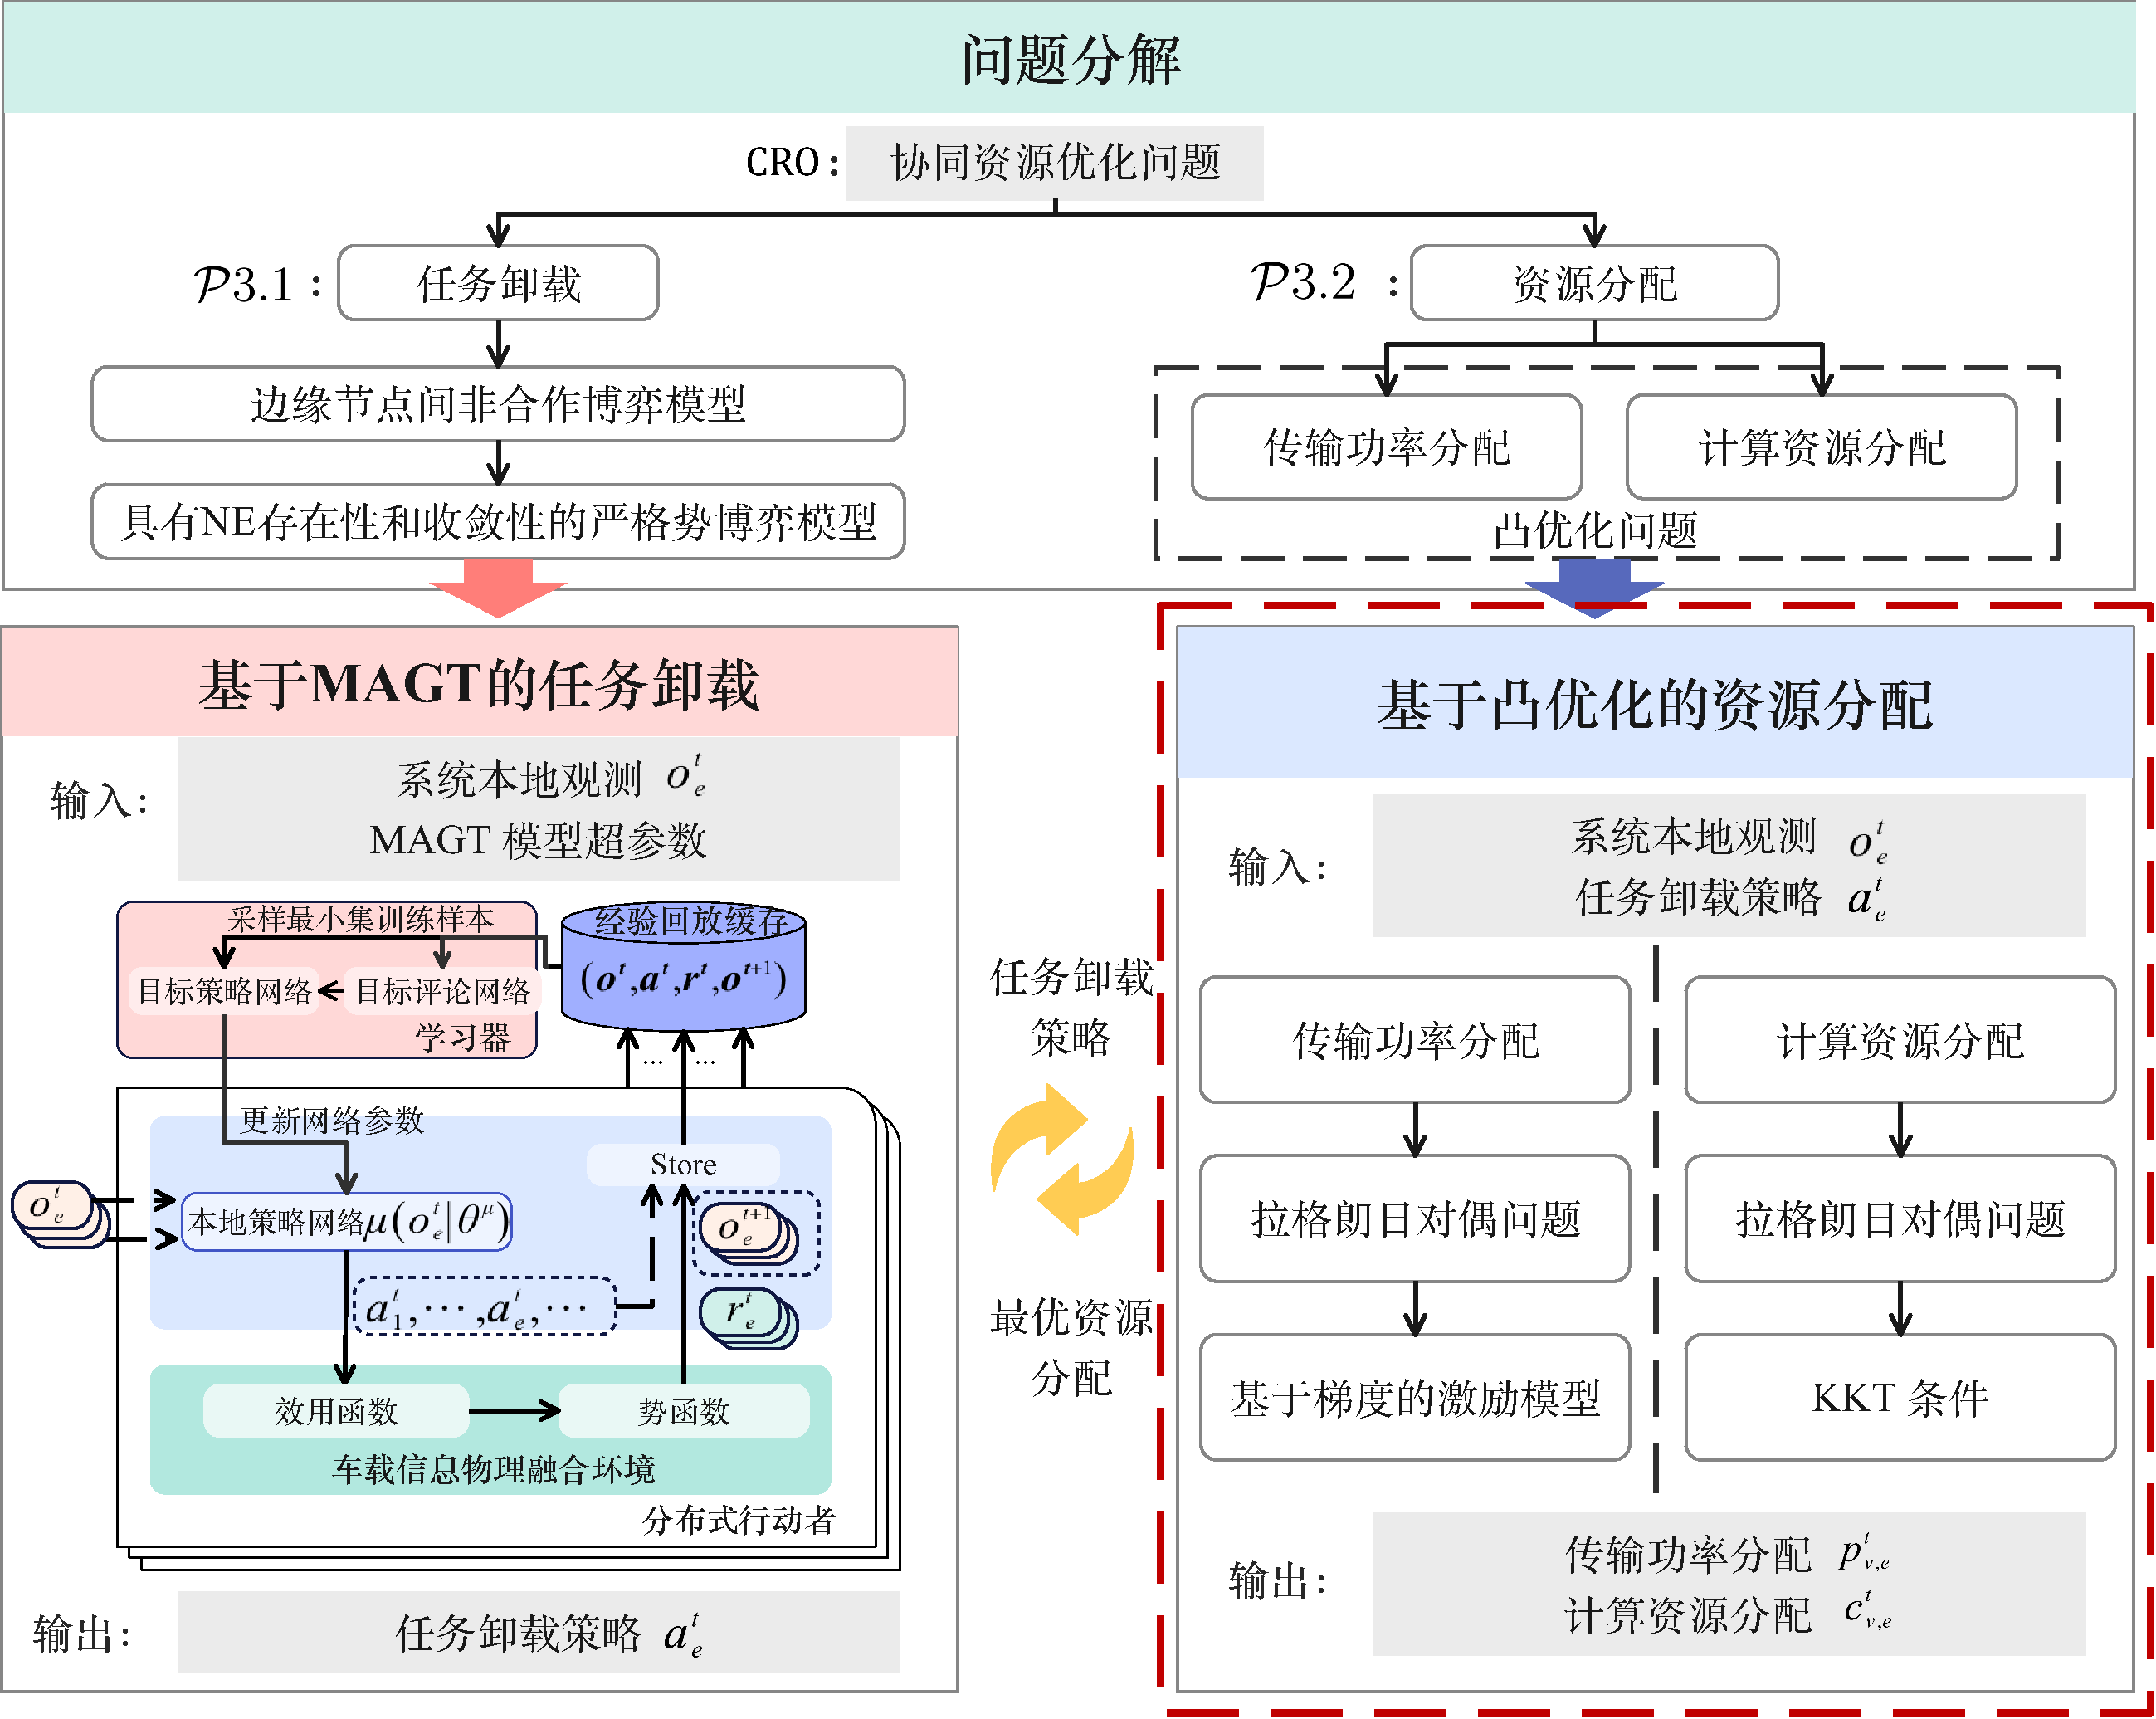
\includegraphics[width=0.45\textwidth]{fig/Fig3-3-solution-model3.pdf}
\end{figure}
\end{textblock*}
\end{center}

\begin{center}
\begin{textblock*}{0.62\textwidth}(0.5cm,2cm)
\begin{itemize}[itemsep=0.2\baselineskip]  \englishfont
	\item[\ding{111}] {\color{cqublue}{传输功率分配}}
	\begin{itemize}[itemsep=0.2\baselineskip] 
	\begin{small}	
	\item[\ding{226}] 引入拉格朗日乘子
	\item $\mathcal{L}(\widetilde{\mathbf{{P}}_{e}^{t}}, {\lambda}_{e}^{t} ) = \widetilde{g_3^{e}} -  {\lambda}_{e}^{t} (\sum_{\forall v \in \mathbf{V}_{e}^{t}} 2^{\widetilde{p_{v, e}^{t}}} - p_{e} )$ 
	\item[\ding{226}] 对偶问题分解为{\color{cqublue}{两层优化问题}}
	\item[\ding{226}] \underline{外层}:固定$\widetilde{\mathbf{{P}}_{e}^{t}}$,优化${\lambda}_{e}^{t}$,梯度下降迭代更新
	\item[\ding{226}] \underline{内层}:固定${\lambda}_{e}^{t}$,优化$\widetilde{\mathbf{{P}}_{e}^{t}}$,寻找拉格朗日静止点
	\end{small}
	\end{itemize}
	\item[\ding{111}] {\color{cqublue}{计算资源分配}}
	\begin{itemize}[itemsep=0.2\baselineskip]  \small
			\item[\ding{226}] 基于KKT条件得到最优解
			\item ${c_{v, e}^{t}}^{\star} = \frac{1 / c_e \sqrt{d_k  c_k} } {\sum_{\forall k_{v}^{t} \in {\mathbf{K}_{q_e}^{t} }} 1 / c_e \sqrt{d_k  c_k}} , \forall k_{v}^{t} \in {\mathbf{K}_{q_e}^{t} } $
			\item 
		\end{itemize}
\end{itemize}
\end{textblock*}
\end{center}
\end{frame}

\begin{frame}
\frametitle{\englishfont \underline{实验}:数据与基本设置}
\newBackground
\begin{center}
	\begin{textblock*}{\textwidth}(-3.2cm,2.7cm)
	\begin{table}[h] \englishfont
\resizebox{0.5\textwidth}{!}{%
\begin{tabular}{cc}
\toprule 
\textbf{参数} & \textbf{值}         \\ \midrule
边缘节点计算能力      & {[}3, 10{]} GHz \\
请求任务大小        & {[}0.01, 5{]} MB               \\
有线传输速率       & 50 Mbps           \\
处理1 bit所需计算资源          & 500 cycles/bit              \\
V2I 带宽& 20 MHz\\
最大传输功率& 1$\times 10^3$ mW\\
策略网络         & 5 层全连接 (隐藏层 256-256-256)  \\
评论家网络         & 5 层全连接 (隐藏层 512-512-256) \\
学习率         & 1$\times10^{-4}$              \\
折扣因子        & 0.996              \\
经验回放缓存大小    & 1$\times10^{6}$          \\
批大小         & 256                \\ \bottomrule
\end{tabular}%
}
\end{table}
\end{textblock*}
\end{center}

\begin{center}
\begin{textblock*}{\textwidth}(0cm,1.8cm)
\begin{itemize} \englishfont 
	\item[\ding{111}] {\color{cqublue}{实验与模型参数}}
\end{itemize}
\end{textblock*}
\end{center}

\begin{center}
\begin{textblock*}{0.65\textwidth}(7.5cm,1.8cm)
\begin{itemize}[itemsep=0.2\baselineskip]  \englishfont 
	\item[\ding{111}] {\color{cqublue}{对比算法}}
	\begin{itemize}[itemsep=0.2\baselineskip] 
	\begin{small}
		\item[\ding{226}] 最优资源分配和任务全迁移 ({\color{red}{ORM}})
		\item[\ding{226}] 最优资源分配和任务仅本地处理 ({\color{red}{ORL}})
		\item[\ding{226}] 分布式深度确定性策略梯度 ({\color{red}{D4PG}})
		\item[\ding{226}] 多智能体深度确定性策略梯度 ({\color{red}{MADDPG}})
		\item
	\end{small}
	\end{itemize}
\end{itemize}
\end{textblock*}
\end{center}

\begin{center}
\begin{textblock*}{0.55\textwidth}(7.5cm,4.5cm)
\begin{itemize}[itemsep=0.2\baselineskip] \englishfont
	\item[\ding{111}] {\color{cqublue}{性能评估指标}}
	\begin{itemize}[itemsep=0.2\baselineskip]
	\begin{small}
		\item[\ding{226}] 累计奖励 ({\color{red}{CR}})
		\item[\ding{226}] 平均服务率 ({\color{red}{ASR}})
		\item[\ding{226}] 平均实现势 ({\color{red}{AAP}})\\
			{\small{$\operatorname{AAP} = \frac{1}{E}\sum_{\forall e \in \mathbf{E}} \sum_{\forall t \in \mathbf{T}} r_{e}^{t}$}}
		\item[\ding{226}] 本地处理与迁移的比例 ({\color{red}{PLPM}})\\
{\small{$P_{\operatorname{local}} = \frac{K_{\operatorname{local}}}{K_{\operatorname{total}}}$}} \hspace{1em}{\small{$P_{\operatorname{migrated}} = \frac{K_{\operatorname{migrated}}}{K_{\operatorname{total}}}$}}
	\end{small}
	\end{itemize}
\end{itemize}
\end{textblock*}
\end{center}

\end{frame}

\begin{frame}
\newBackground

\begin{overlayarea}{\textwidth}{3cm}
\only<1-1>{
\frametitle{\englishfont \underline{实验}:算法收敛性}
\begin{center} \englishfont \footnotesize
\begin{textblock*}{\textwidth}(1cm,1.8cm)
	\begin{figure}
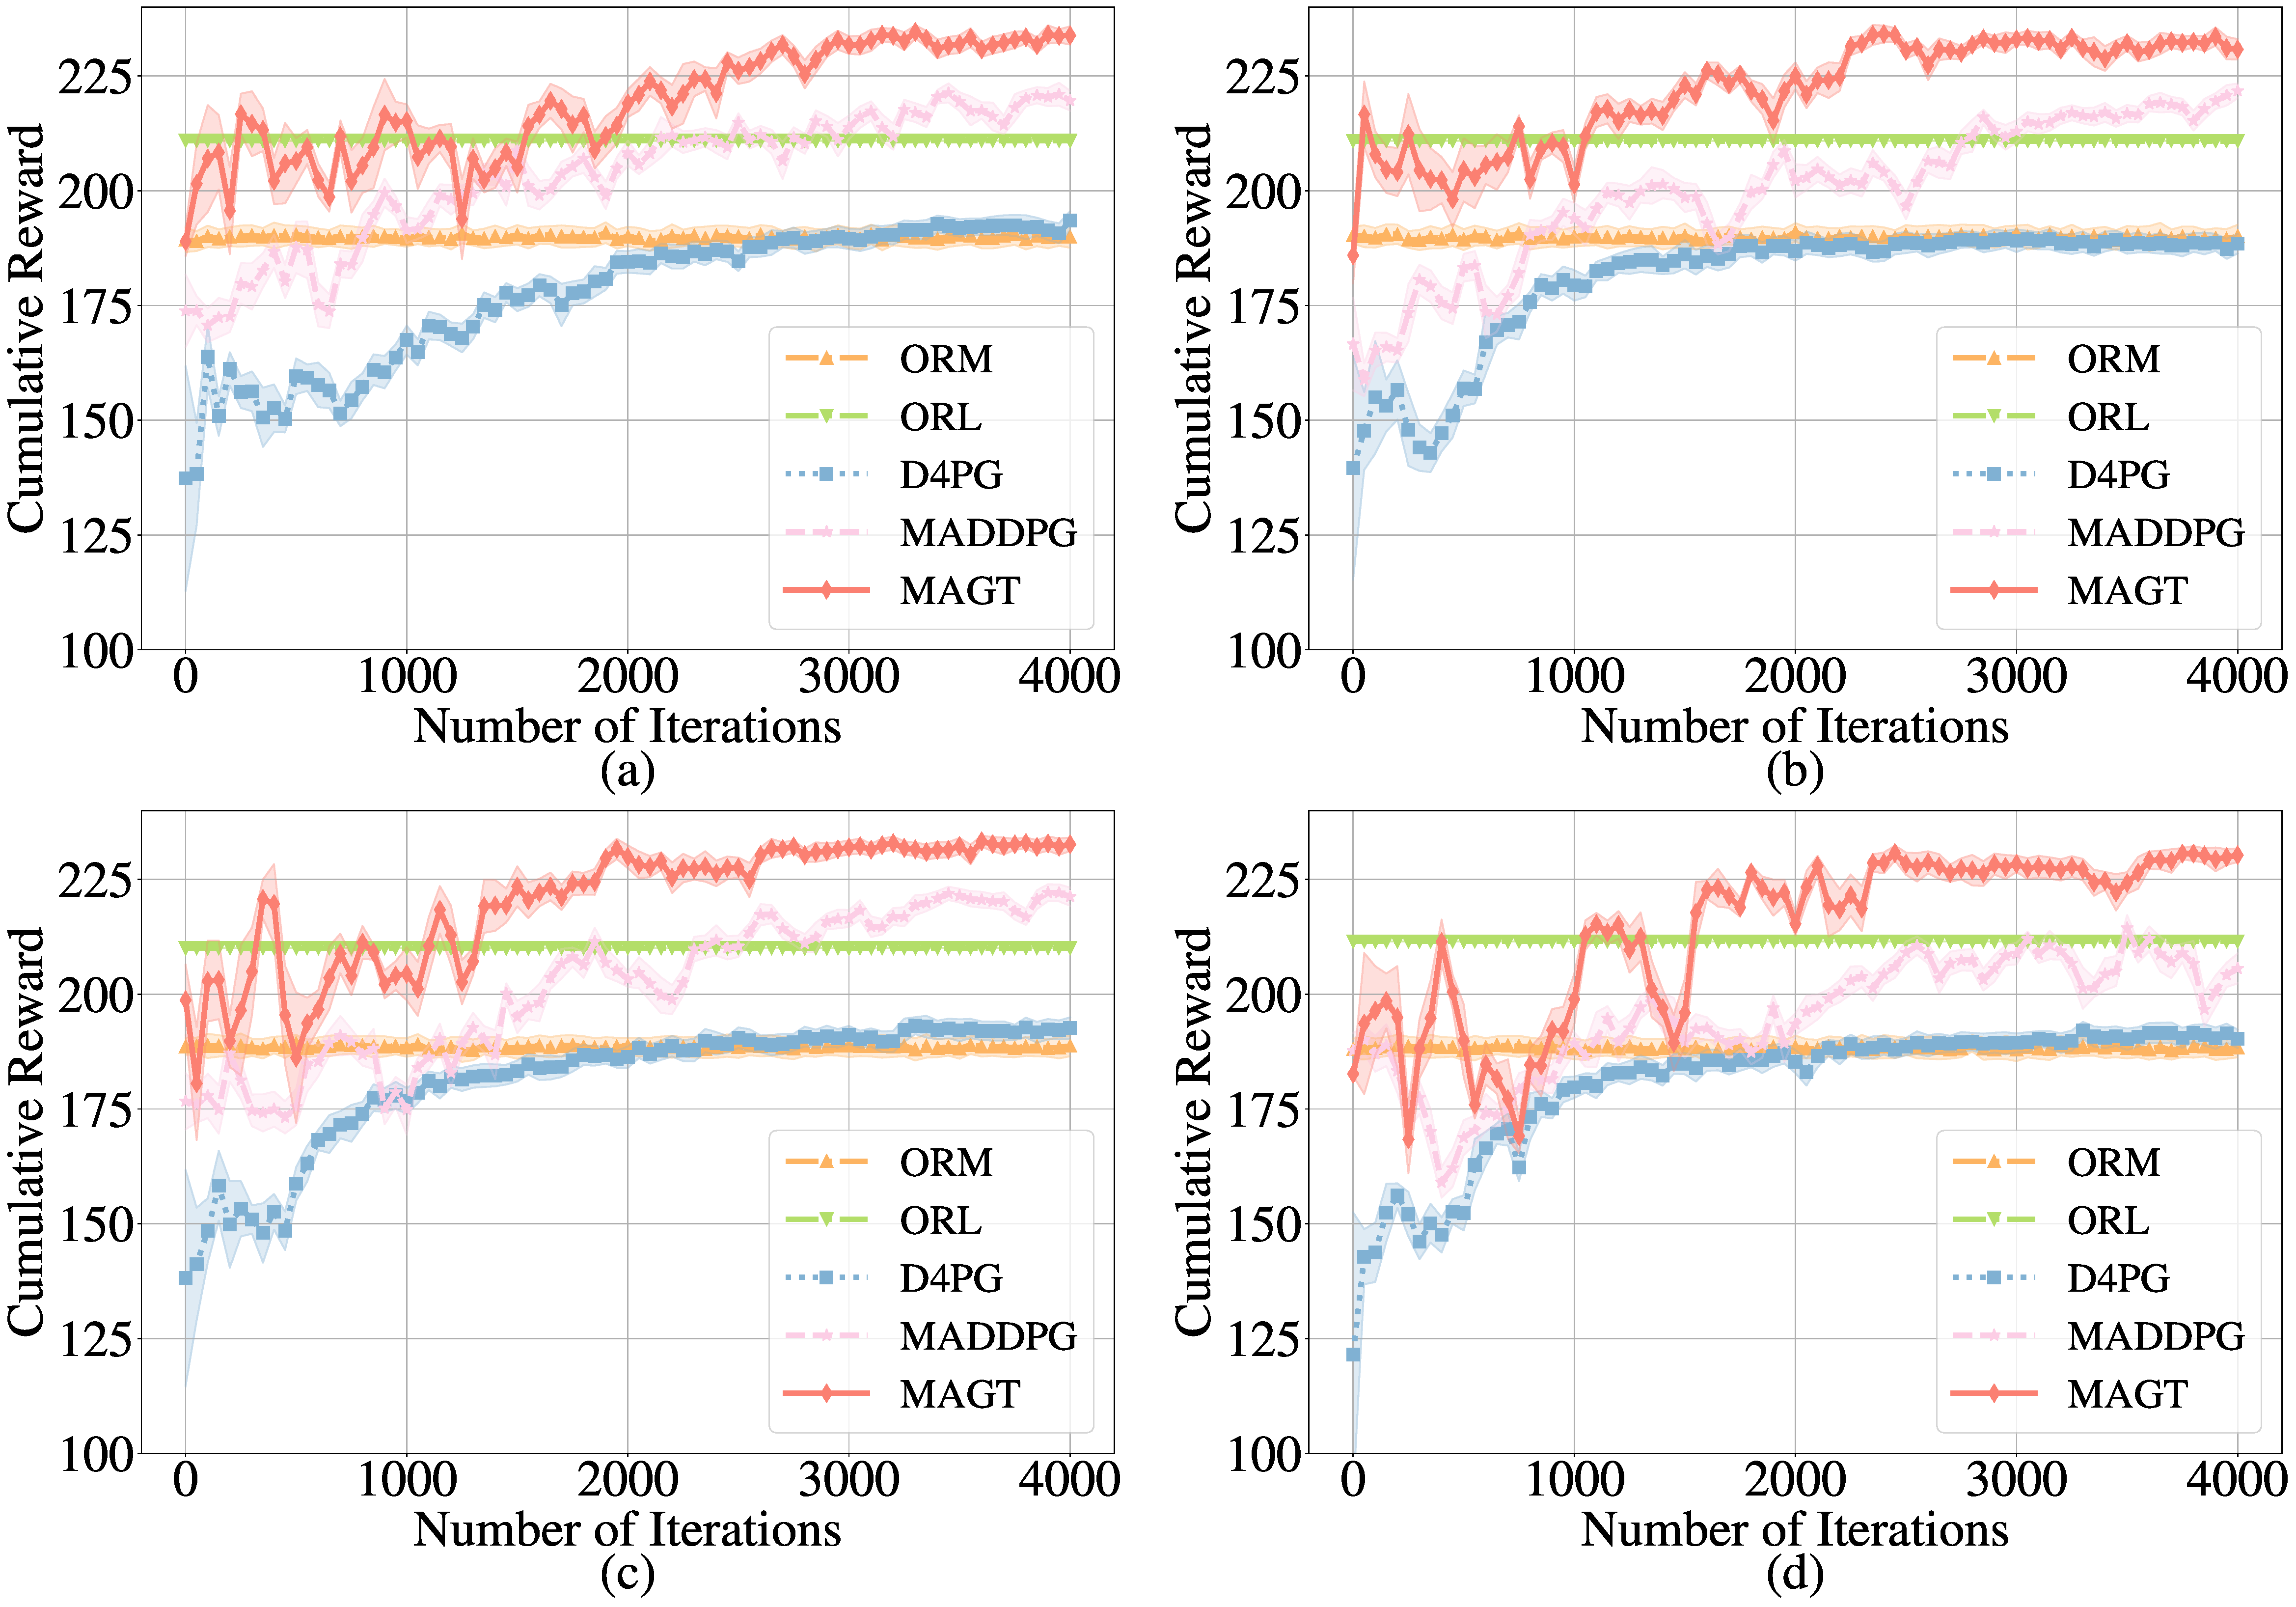
\includegraphics[width=0.65\textwidth]{fig/Fig3-4-convergence.pdf}
	\end{figure}
\end{textblock*}
\end{center}
}

\only<2-2>{
\frametitle{\englishfont \underline{实验}:算法收敛性}
\begin{center} \englishfont \footnotesize
\begin{textblock*}{\textwidth}(1cm,1.8cm)
	\begin{figure}
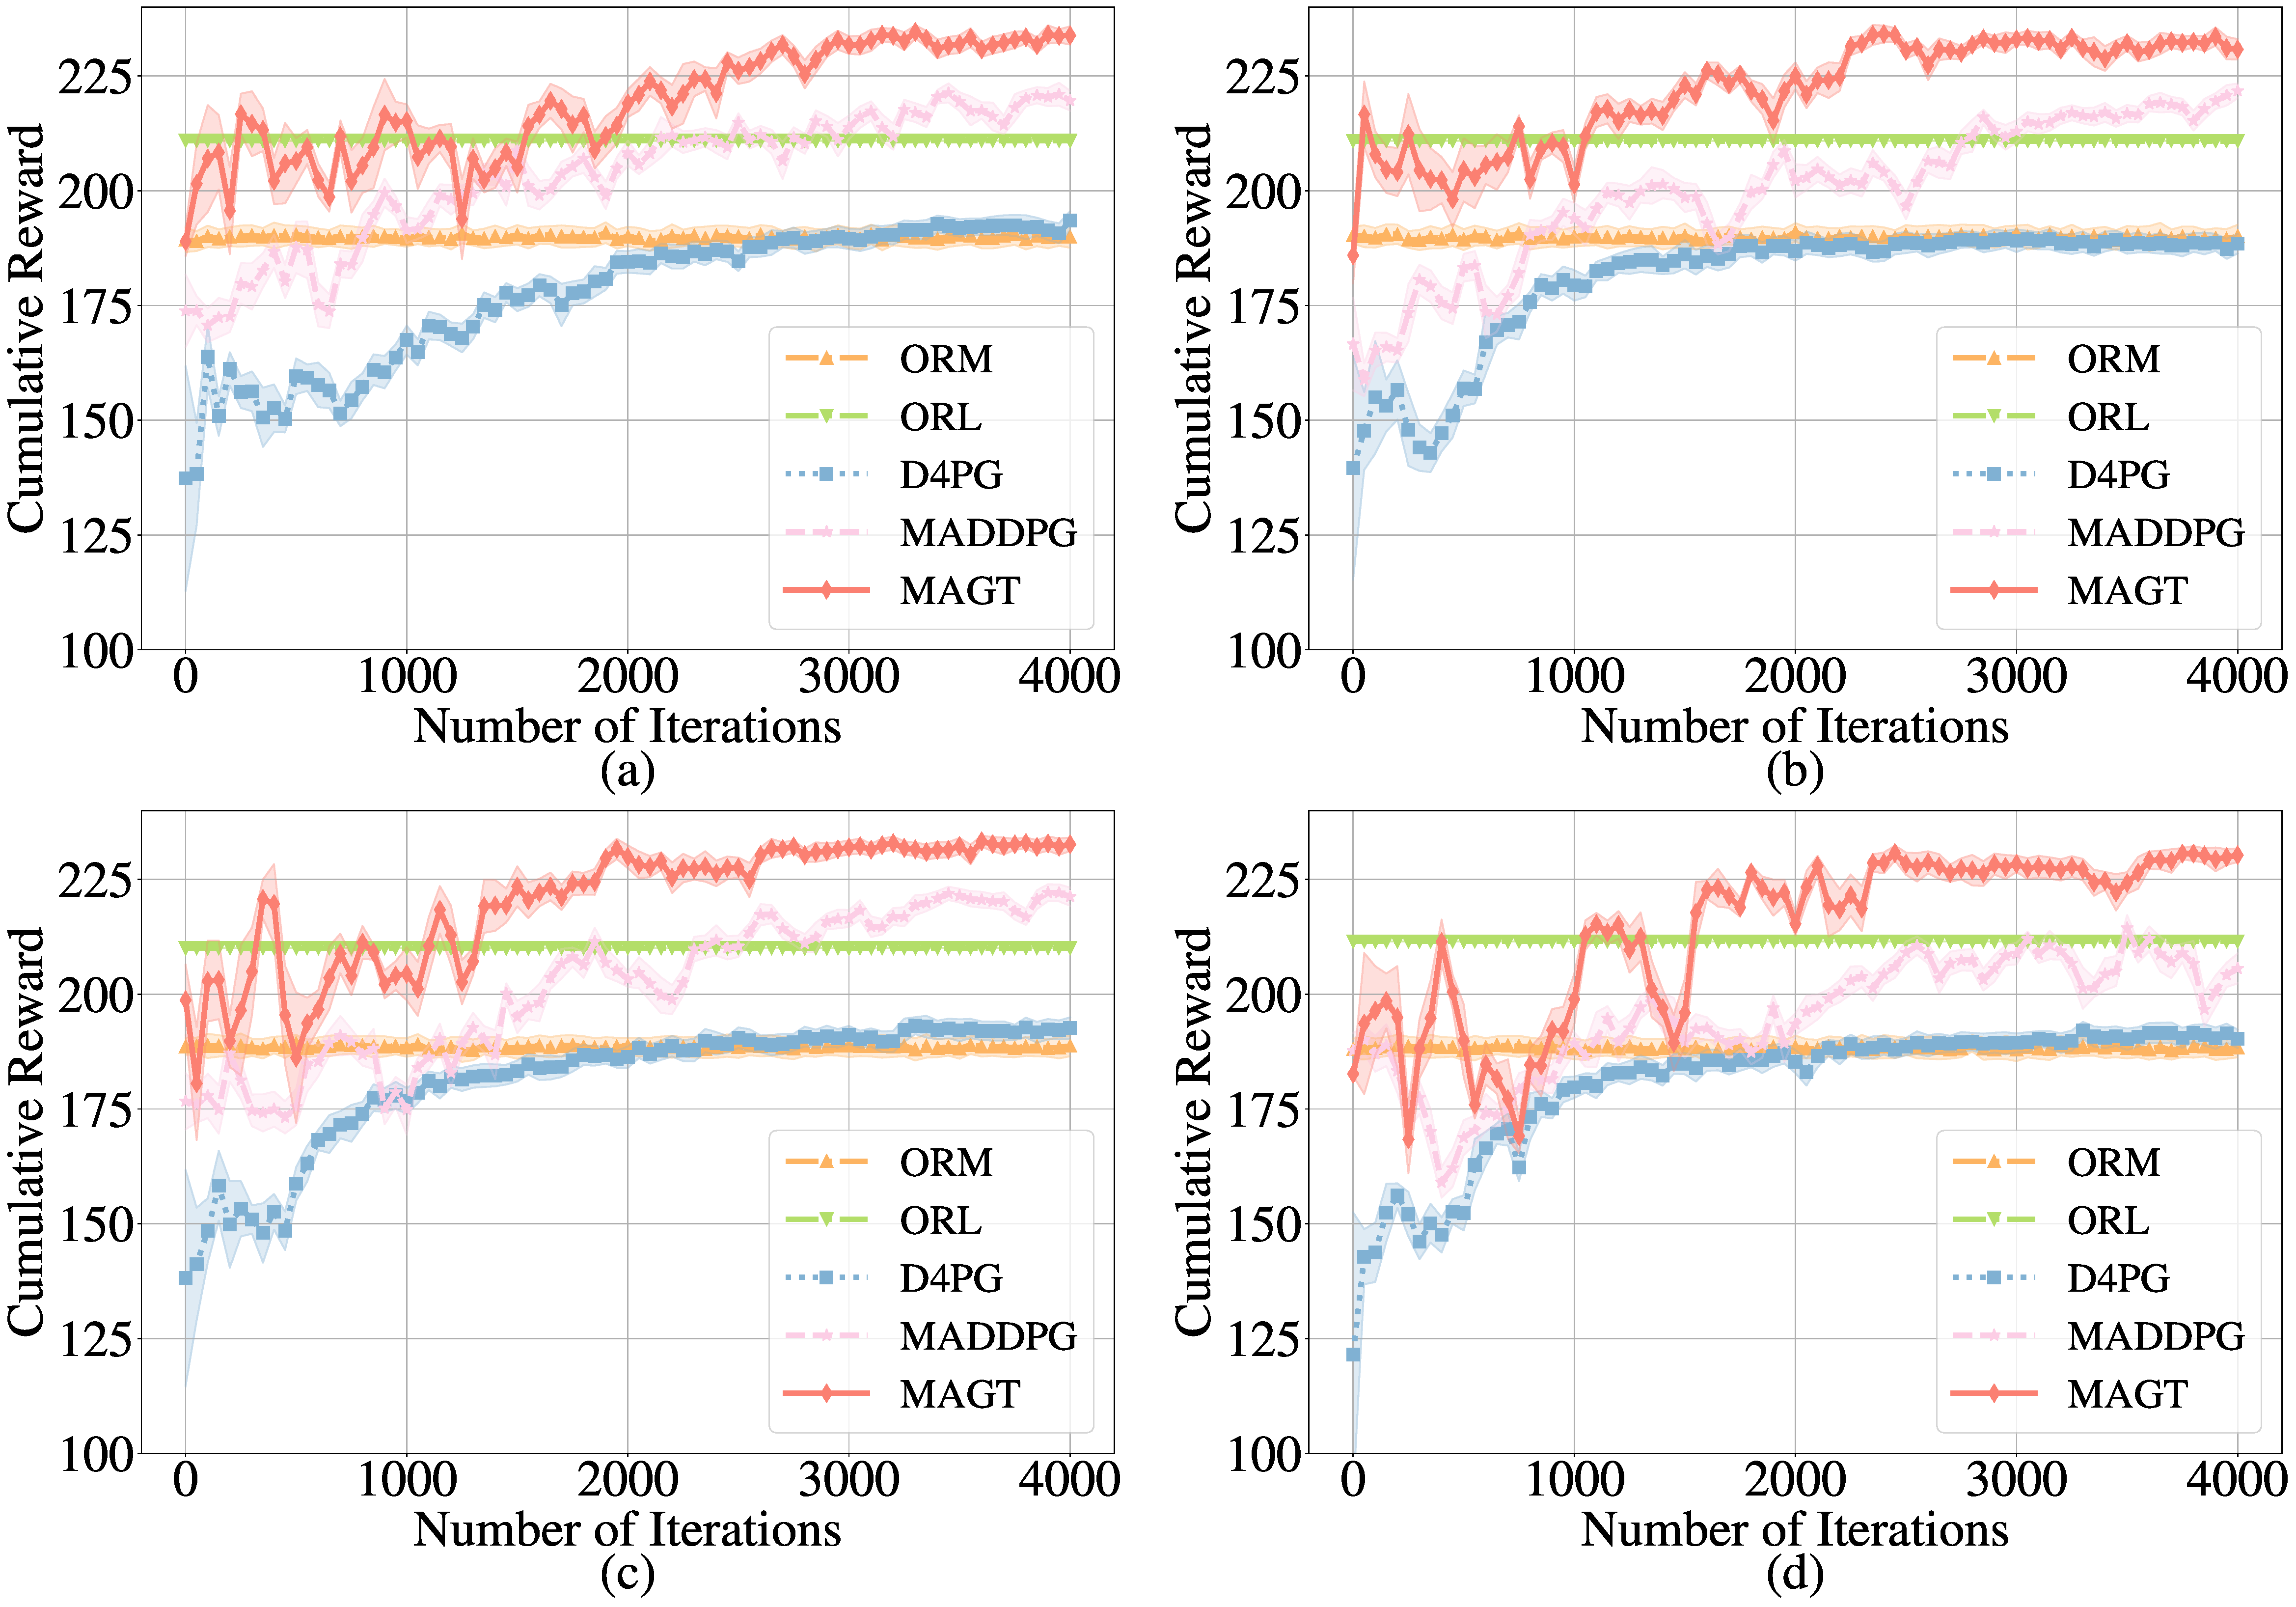
\includegraphics[width=0.65\textwidth]{fig/Fig3-4-convergence.pdf}
	\end{figure}
\end{textblock*}
\end{center}
}

\only<2-2>{
\begin{center} \englishfont \footnotesize
\begin{textblock*}{\textwidth}(0cm,1.6cm)
{\LARGE{\color{red}\ding{216}}}
\end{textblock*}
\end{center}

\begin{center} \englishfont \footnotesize
\begin{textblock*}{\textwidth}(5cm,1.6cm)
{\LARGE{\color{red}\ding{216}}}
\end{textblock*}
\end{center}

\begin{center} \englishfont \footnotesize
\begin{textblock*}{\textwidth}(0cm,4.8cm)
{\LARGE{\color{red}\ding{216}}}
\end{textblock*}
\end{center}

\begin{center} \englishfont \footnotesize
\begin{textblock*}{\textwidth}(5cm,4.8cm)
{\LARGE{\color{red}\ding{216}}}
\end{textblock*}
\end{center}
}

\only<3-3>{
\frametitle{\englishfont \underline{实验}:交通场景的影响}
\begin{center} \englishfont \footnotesize
\begin{textblock*}{\textwidth}(1cm,1.8cm)
	\begin{figure}
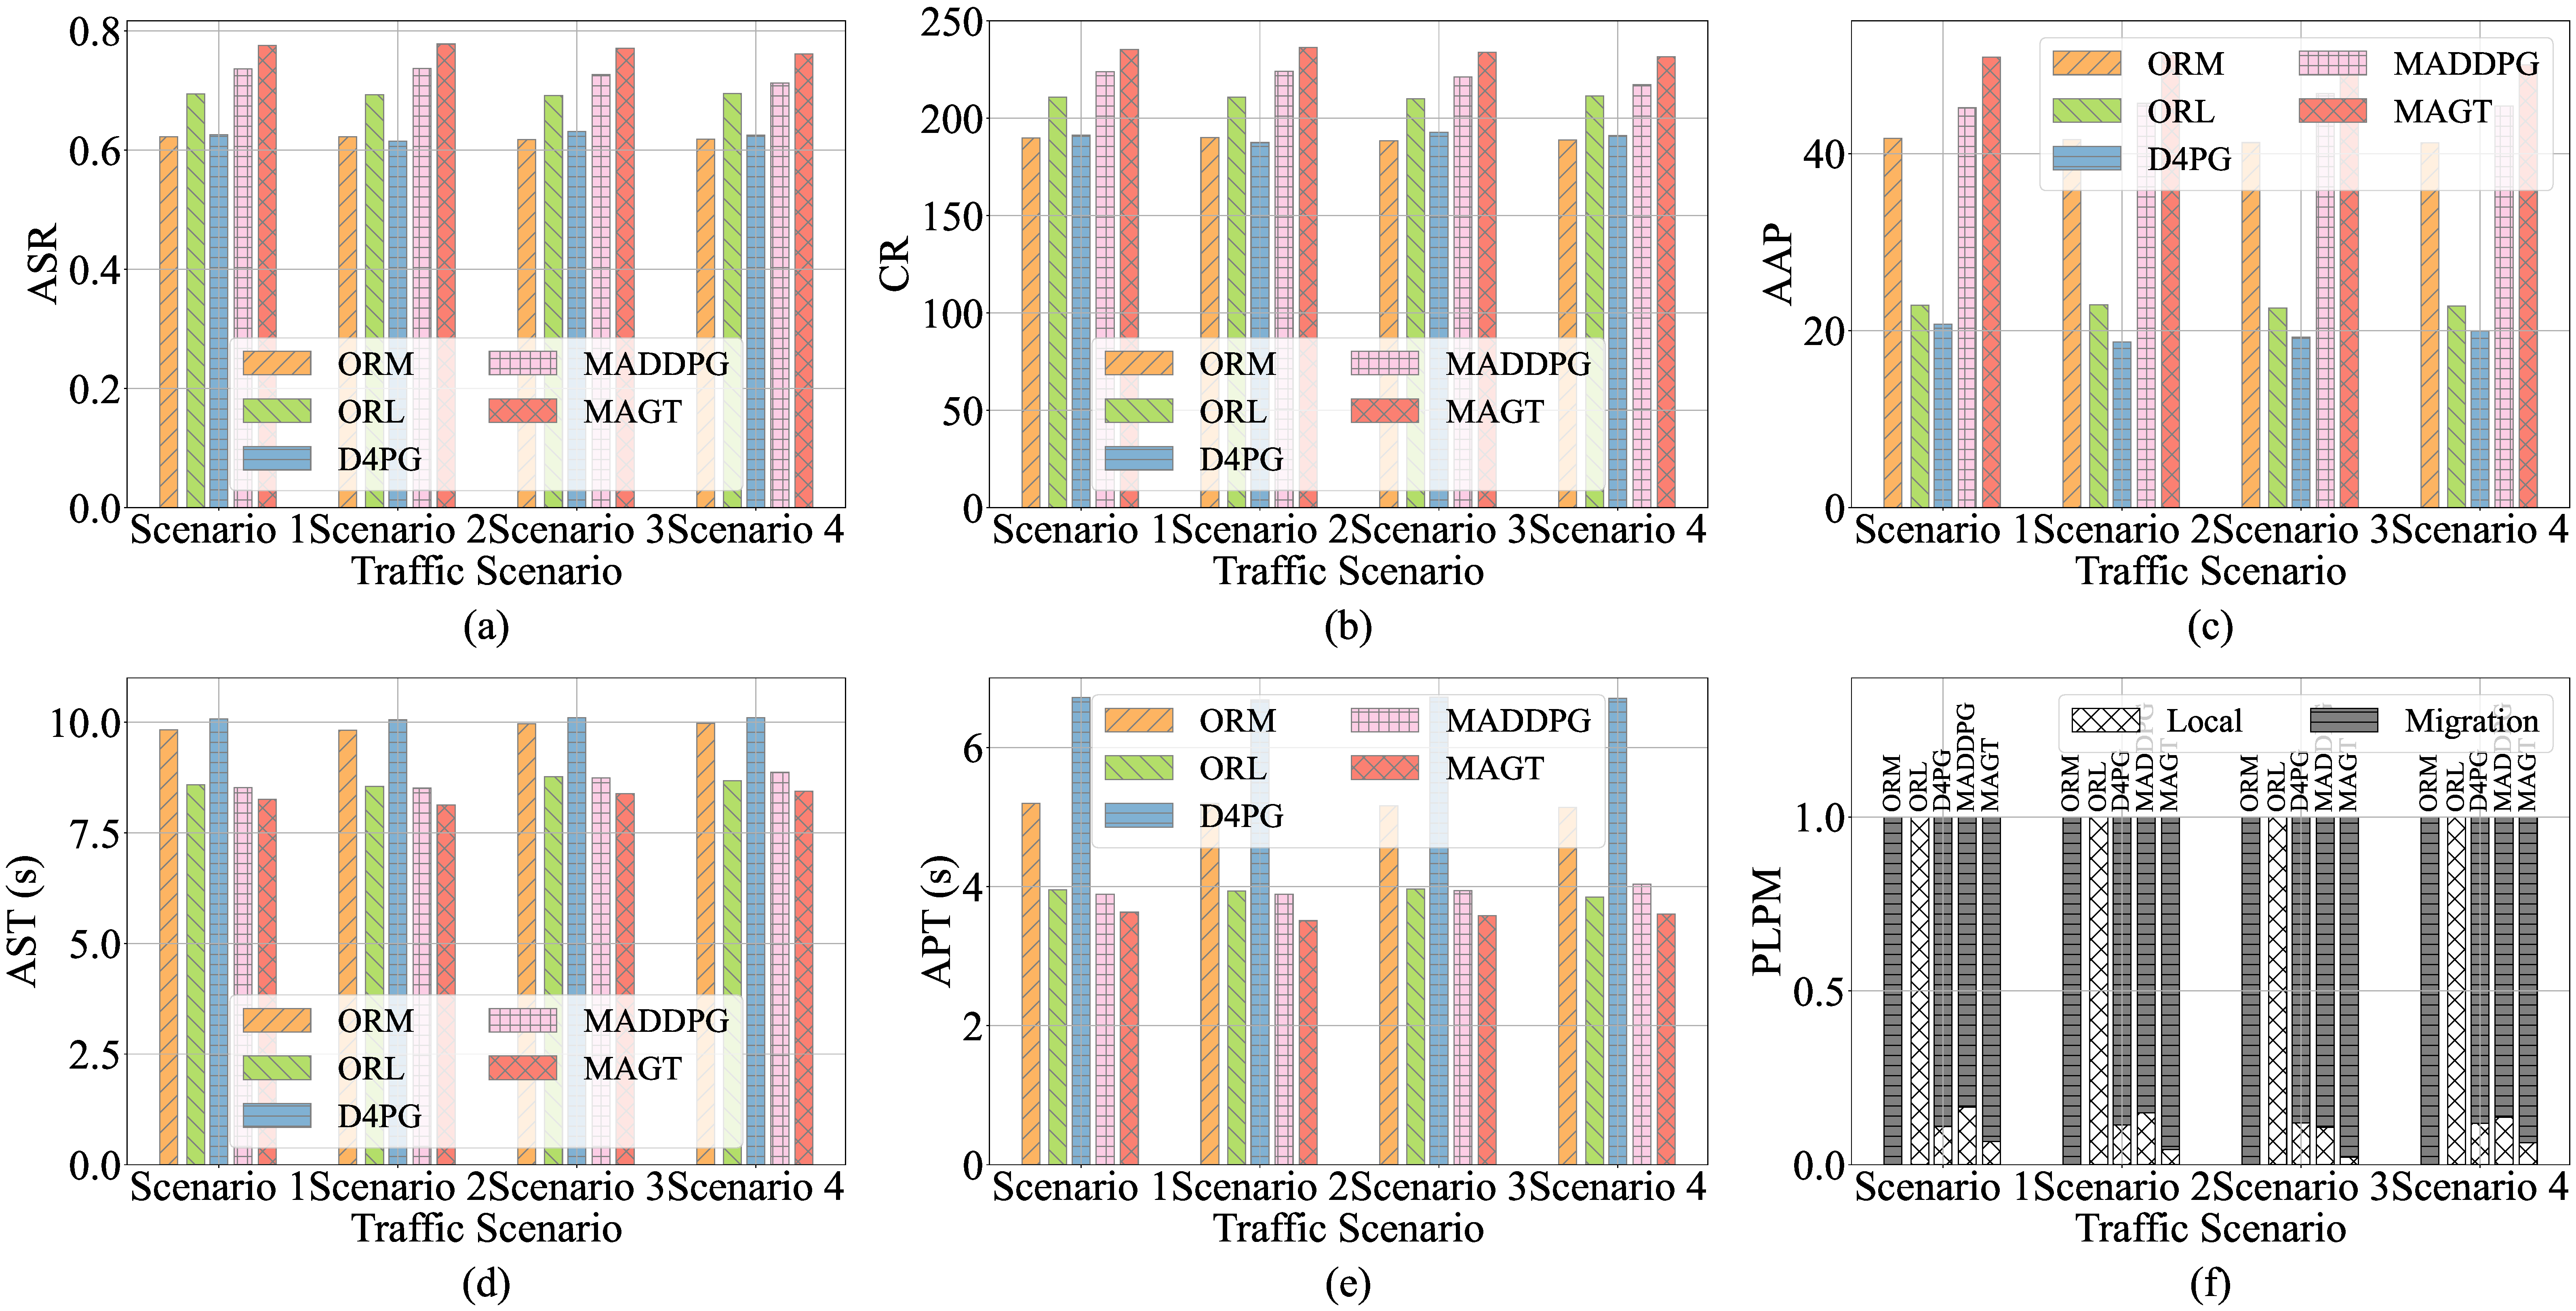
\includegraphics[width=0.9\textwidth]{fig/Fig3-5-different-traffica-scenarios.pdf}
	\end{figure}
\end{textblock*}
\end{center}
}

\only<4-4>{
\frametitle{\englishfont \underline{实验}:交通场景的影响}
\begin{center} \englishfont \footnotesize
\begin{textblock*}{\textwidth}(1cm,1.8cm)
	\begin{figure}
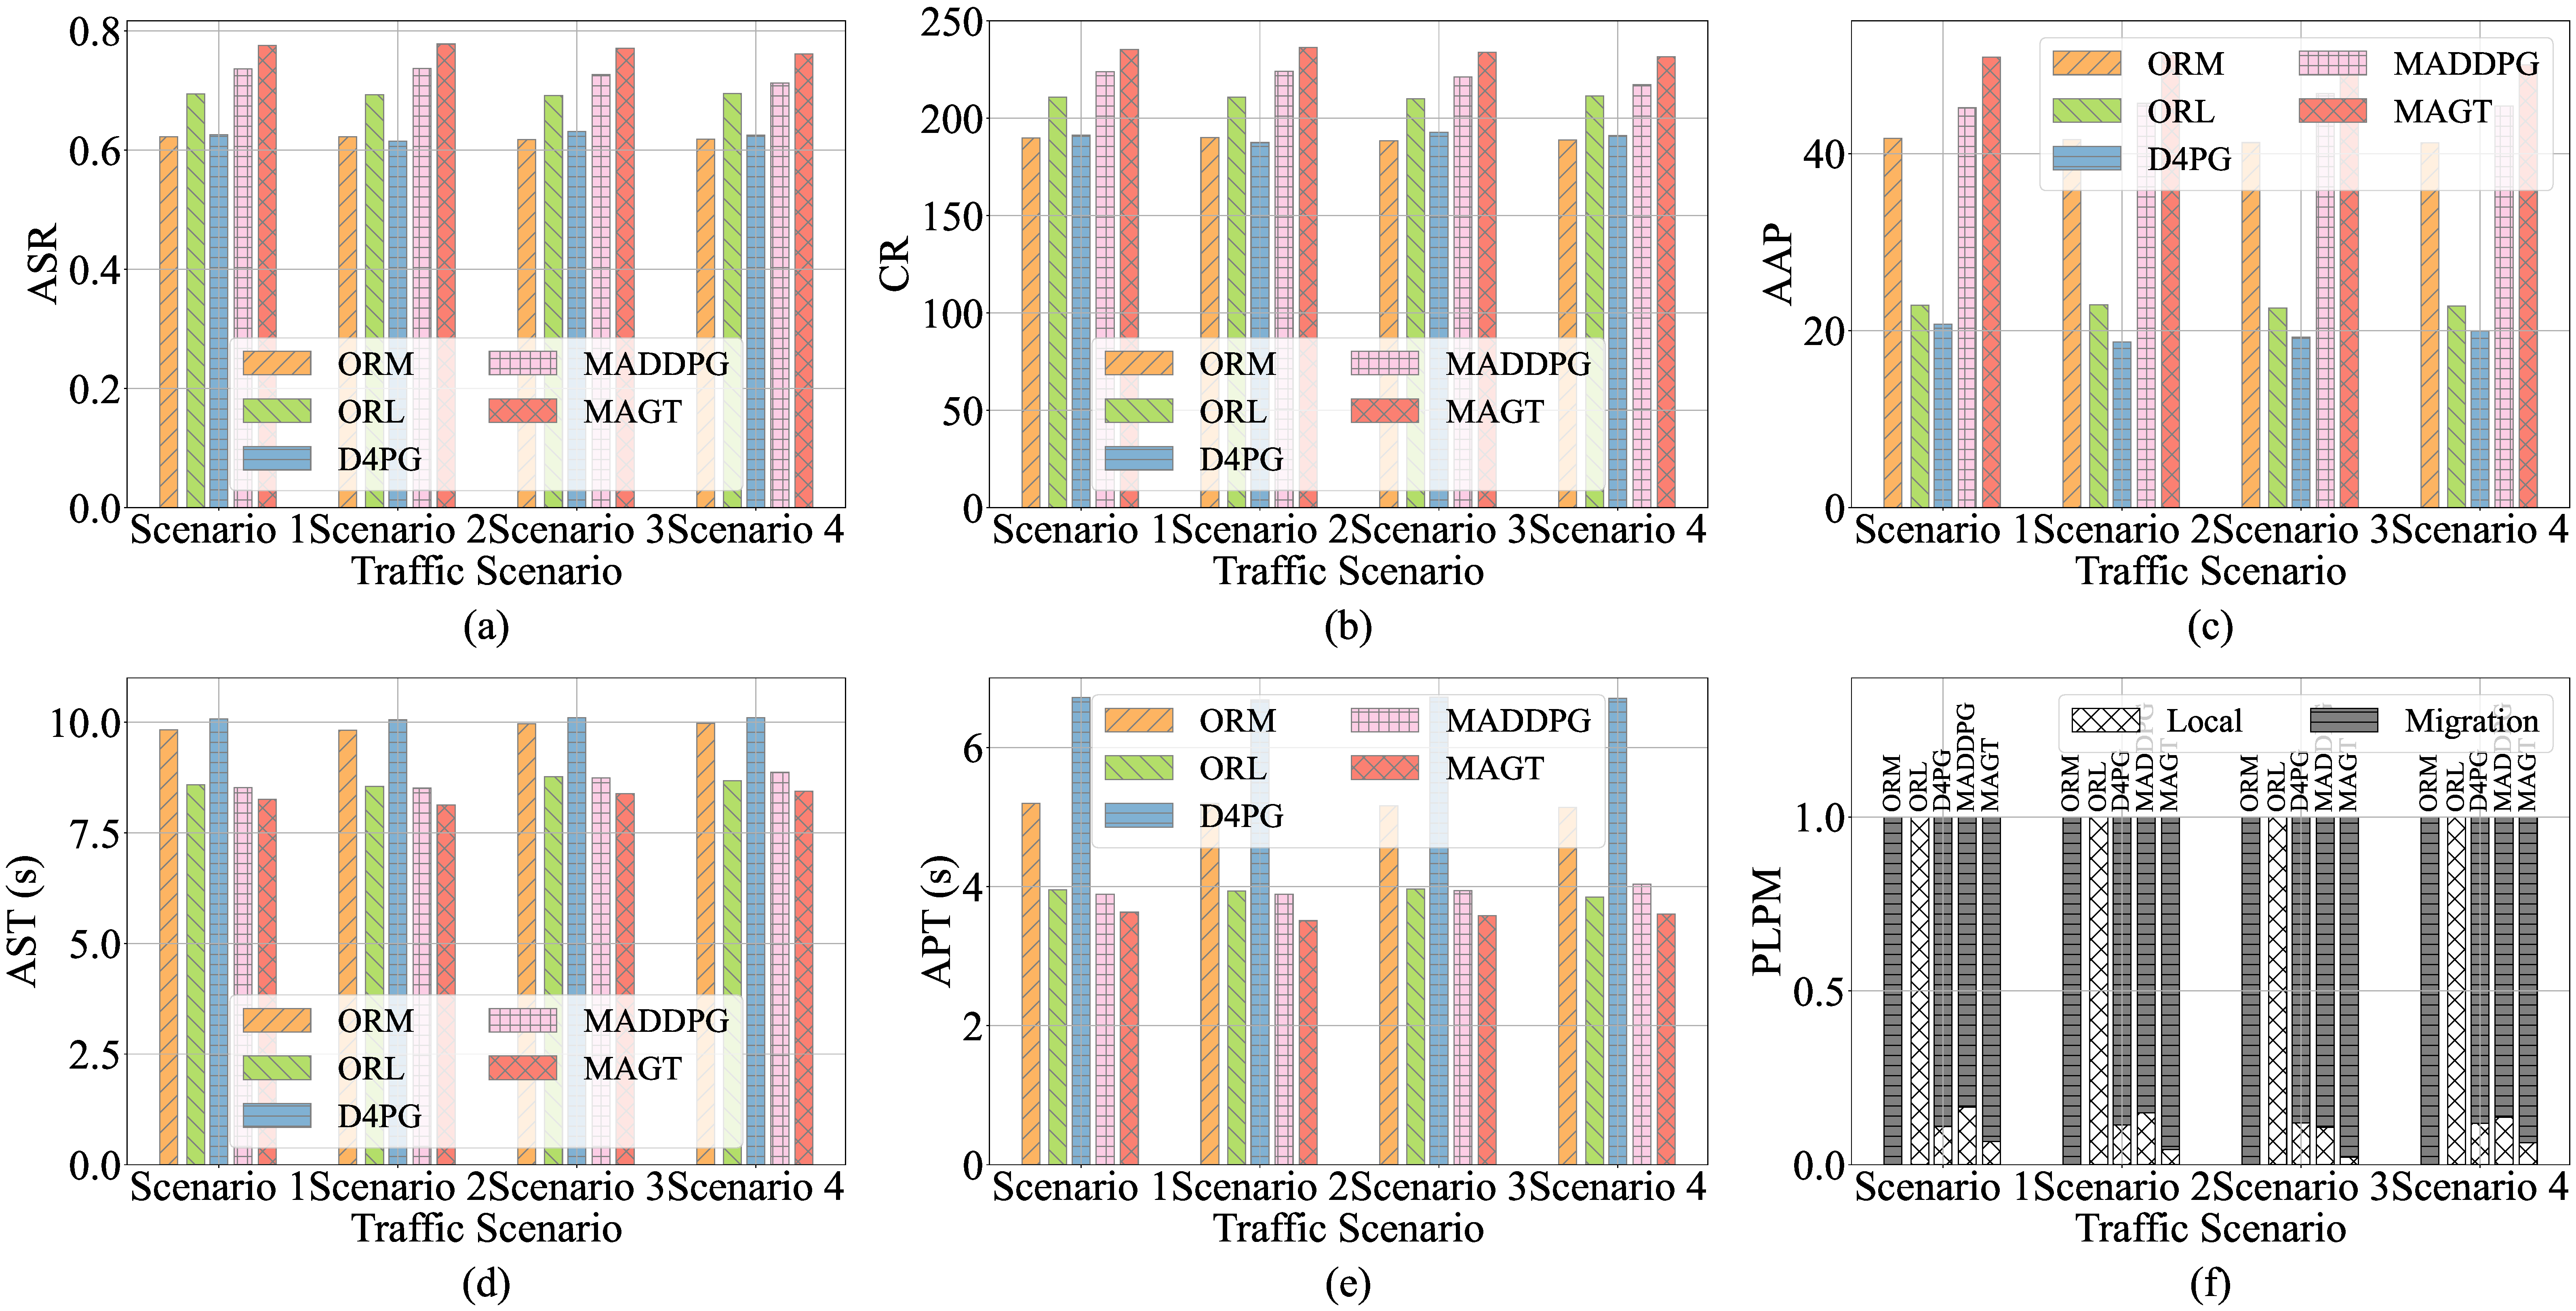
\includegraphics[width=0.9\textwidth]{fig/Fig3-5-different-traffica-scenarios.pdf}
	\end{figure}
\end{textblock*}
\end{center}
}

\only<4-4>{
\begin{center} \englishfont \footnotesize
\begin{textblock*}{\textwidth}(-3.3cm,1.65cm)
{\LARGE{\color{red}\ding{216}}}
\end{textblock*}
\end{center}

\begin{center} \englishfont \footnotesize
\begin{textblock*}{\textwidth}(0.9cm,1.7cm)
{\LARGE{\color{red}\ding{216}}}
\end{textblock*}
\end{center}

\begin{center} \englishfont \footnotesize
\begin{textblock*}{\textwidth}(4.25cm,1.75cm)
{\LARGE{\color{red}\ding{216}}}
\end{textblock*}
\end{center}

\begin{center} \englishfont \footnotesize
\begin{textblock*}{\textwidth}(0.9cm,5.95cm)
{\LARGE{\color{red}\ding{216}}}
\end{textblock*}
\end{center}

\begin{center} \englishfont \footnotesize
\begin{textblock*}{\textwidth}(-3.3cm,5.4cm)
{\LARGE{\color{red}\ding{216}}}
\end{textblock*}
\end{center}
}

\only<5-5>{
\frametitle{\englishfont \underline{实验}:计算能力的影响}
\begin{center} \englishfont \footnotesize
\begin{textblock*}{\textwidth}(1cm,1.8cm)
	\begin{figure}
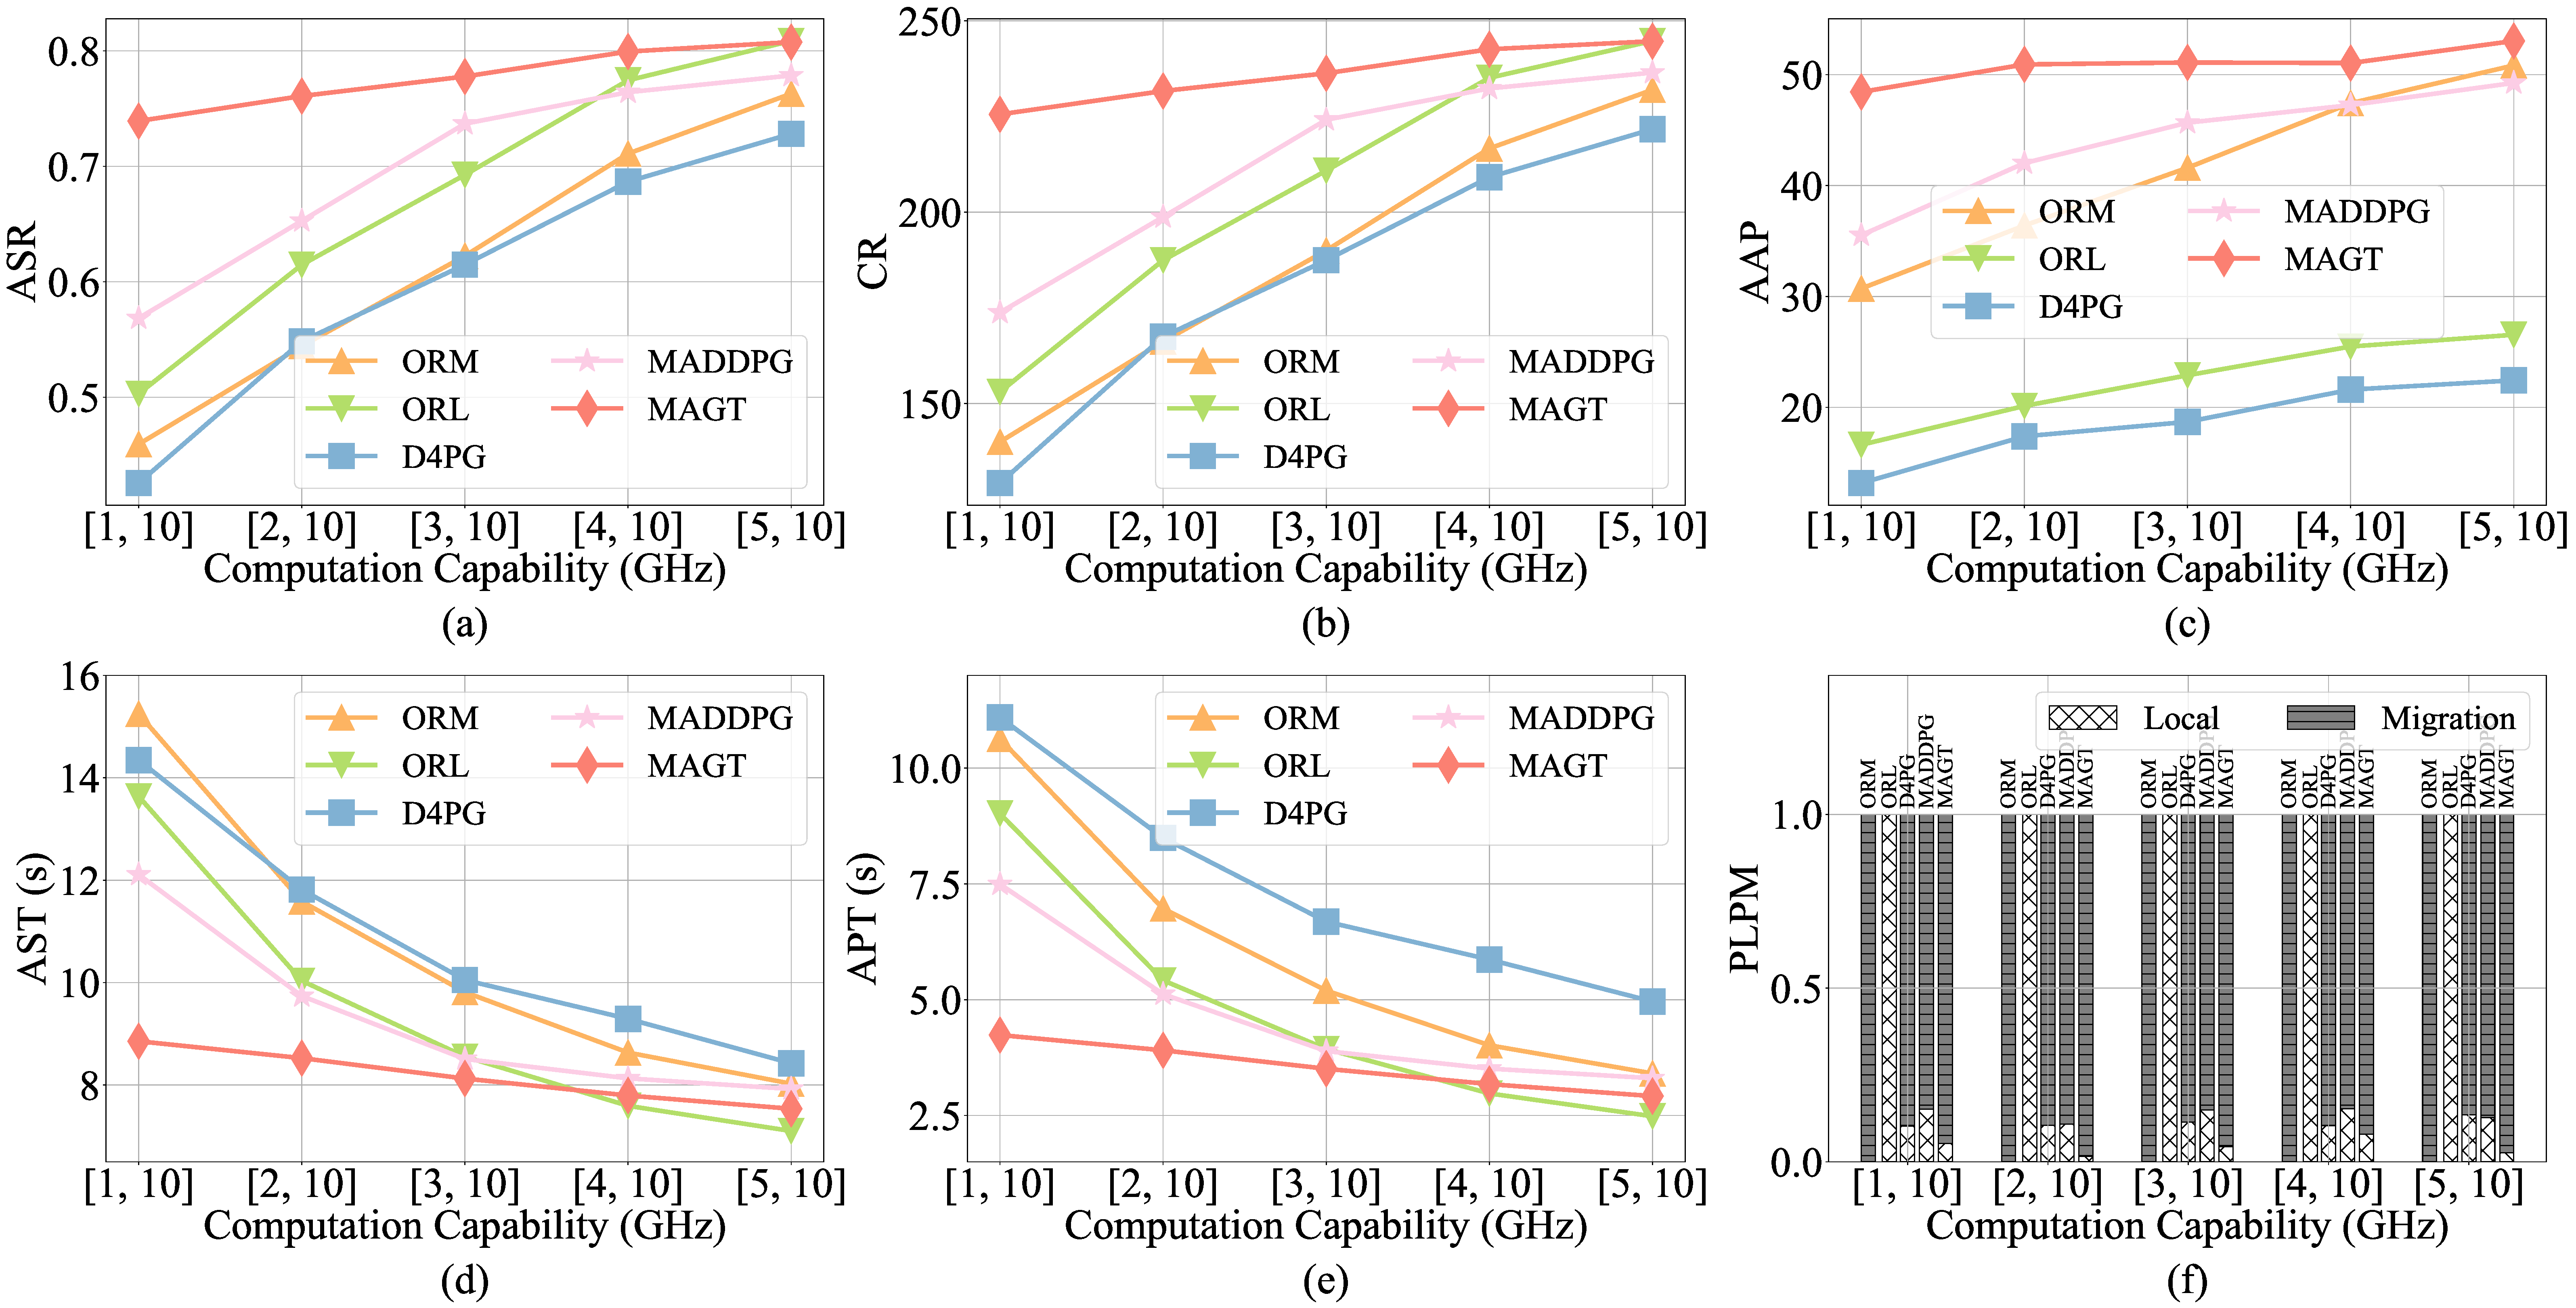
\includegraphics[width=0.9\textwidth]{fig/Fig3-6-different-computation-capability.pdf}
	\end{figure}
\end{textblock*}
\end{center}
}

\only<6-6>{
\frametitle{\englishfont \underline{实验}:计算能力的影响}
\begin{center} \englishfont \footnotesize
\begin{textblock*}{\textwidth}(1cm,1.8cm)
	\begin{figure}
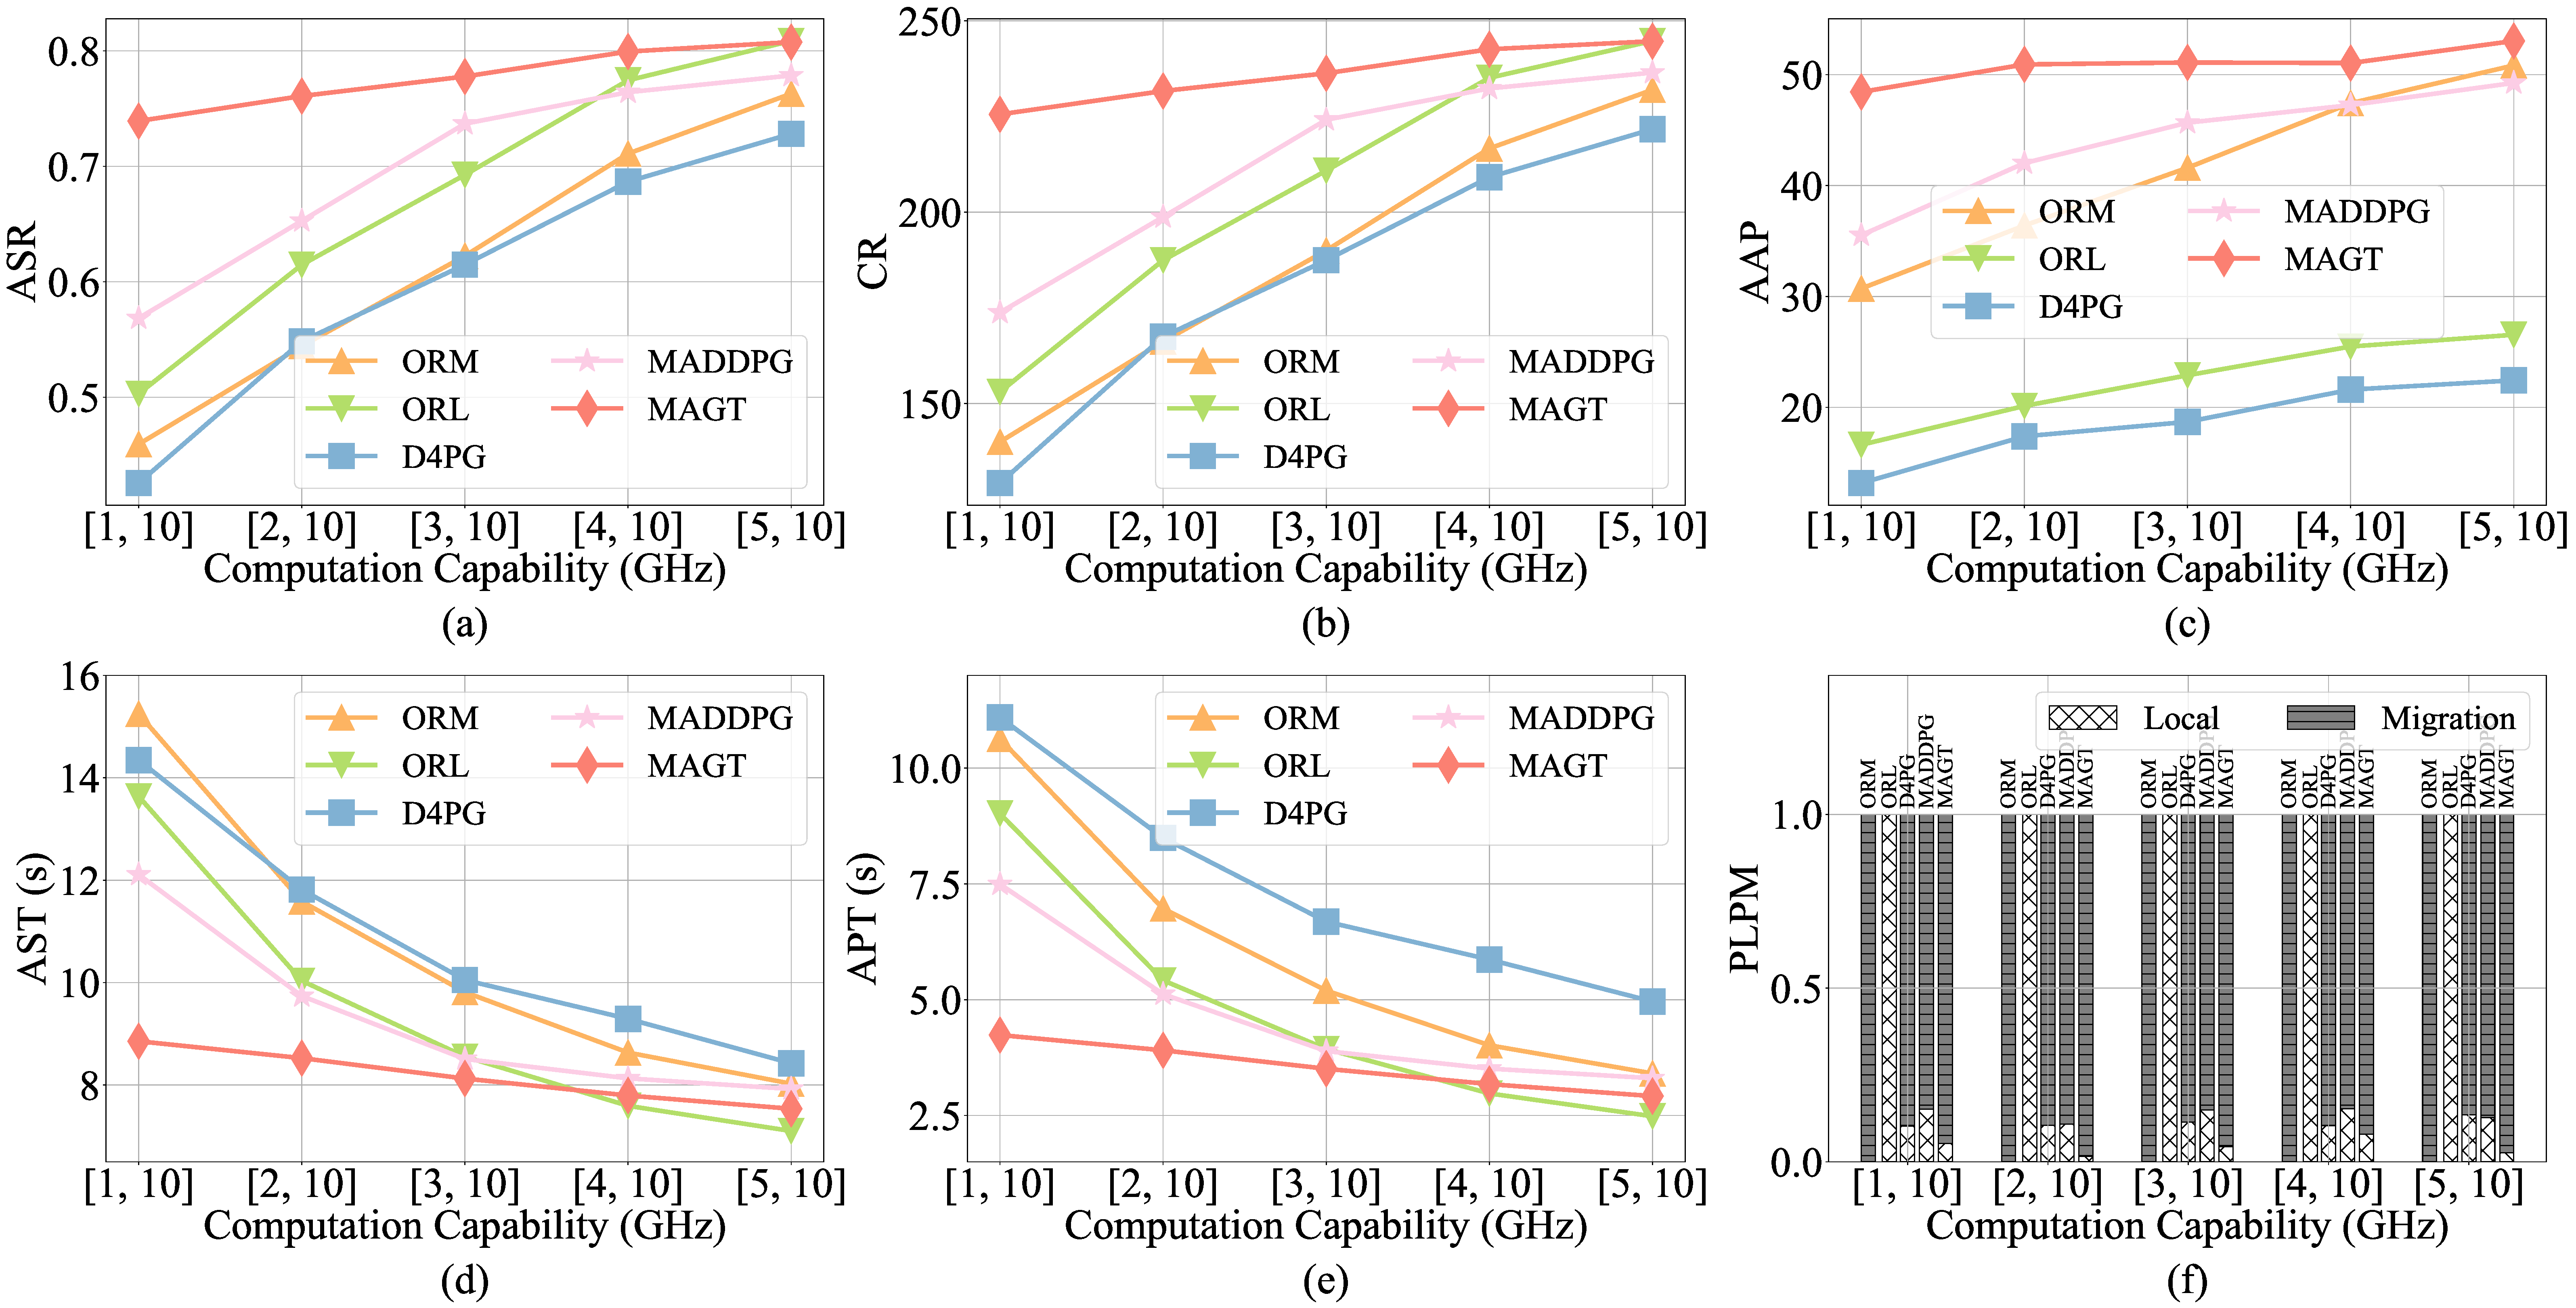
\includegraphics[width=0.9\textwidth]{fig/Fig3-6-different-computation-capability.pdf}
	\end{figure}
\end{textblock*}
\end{center}
}

\only<6-6>{
\begin{center} \englishfont \footnotesize
\begin{textblock*}{\textwidth}(-3.2cm,1.72cm)
{\LARGE{\color{red}\ding{216}}}
\end{textblock*}
\end{center}

\begin{center} \englishfont \footnotesize
\begin{textblock*}{\textwidth}(1cm,1.7cm)
{\LARGE{\color{red}\ding{216}}}
\end{textblock*}
\end{center}

\begin{center} \englishfont \footnotesize
\begin{textblock*}{\textwidth}(5.5cm,1.65cm)
{\LARGE{\color{red}\ding{216}}}
\end{textblock*}
\end{center}

\begin{center} \englishfont \footnotesize
\begin{textblock*}{\textwidth}(0.15cm,6.55cm)
{\LARGE{\color{red}\ding{216}}}
\end{textblock*}
\end{center}

\begin{center} \englishfont \footnotesize
\begin{textblock*}{\textwidth}(-4.2cm,6.5cm)
{\LARGE{\color{red}\ding{216}}}
\end{textblock*}
\end{center}
}

\only<7-7>{
\frametitle{\englishfont \underline{实验}:任务到达概率的影响}
\begin{center} \englishfont \footnotesize
\begin{textblock*}{\textwidth}(1cm,1.8cm)
	\begin{figure}
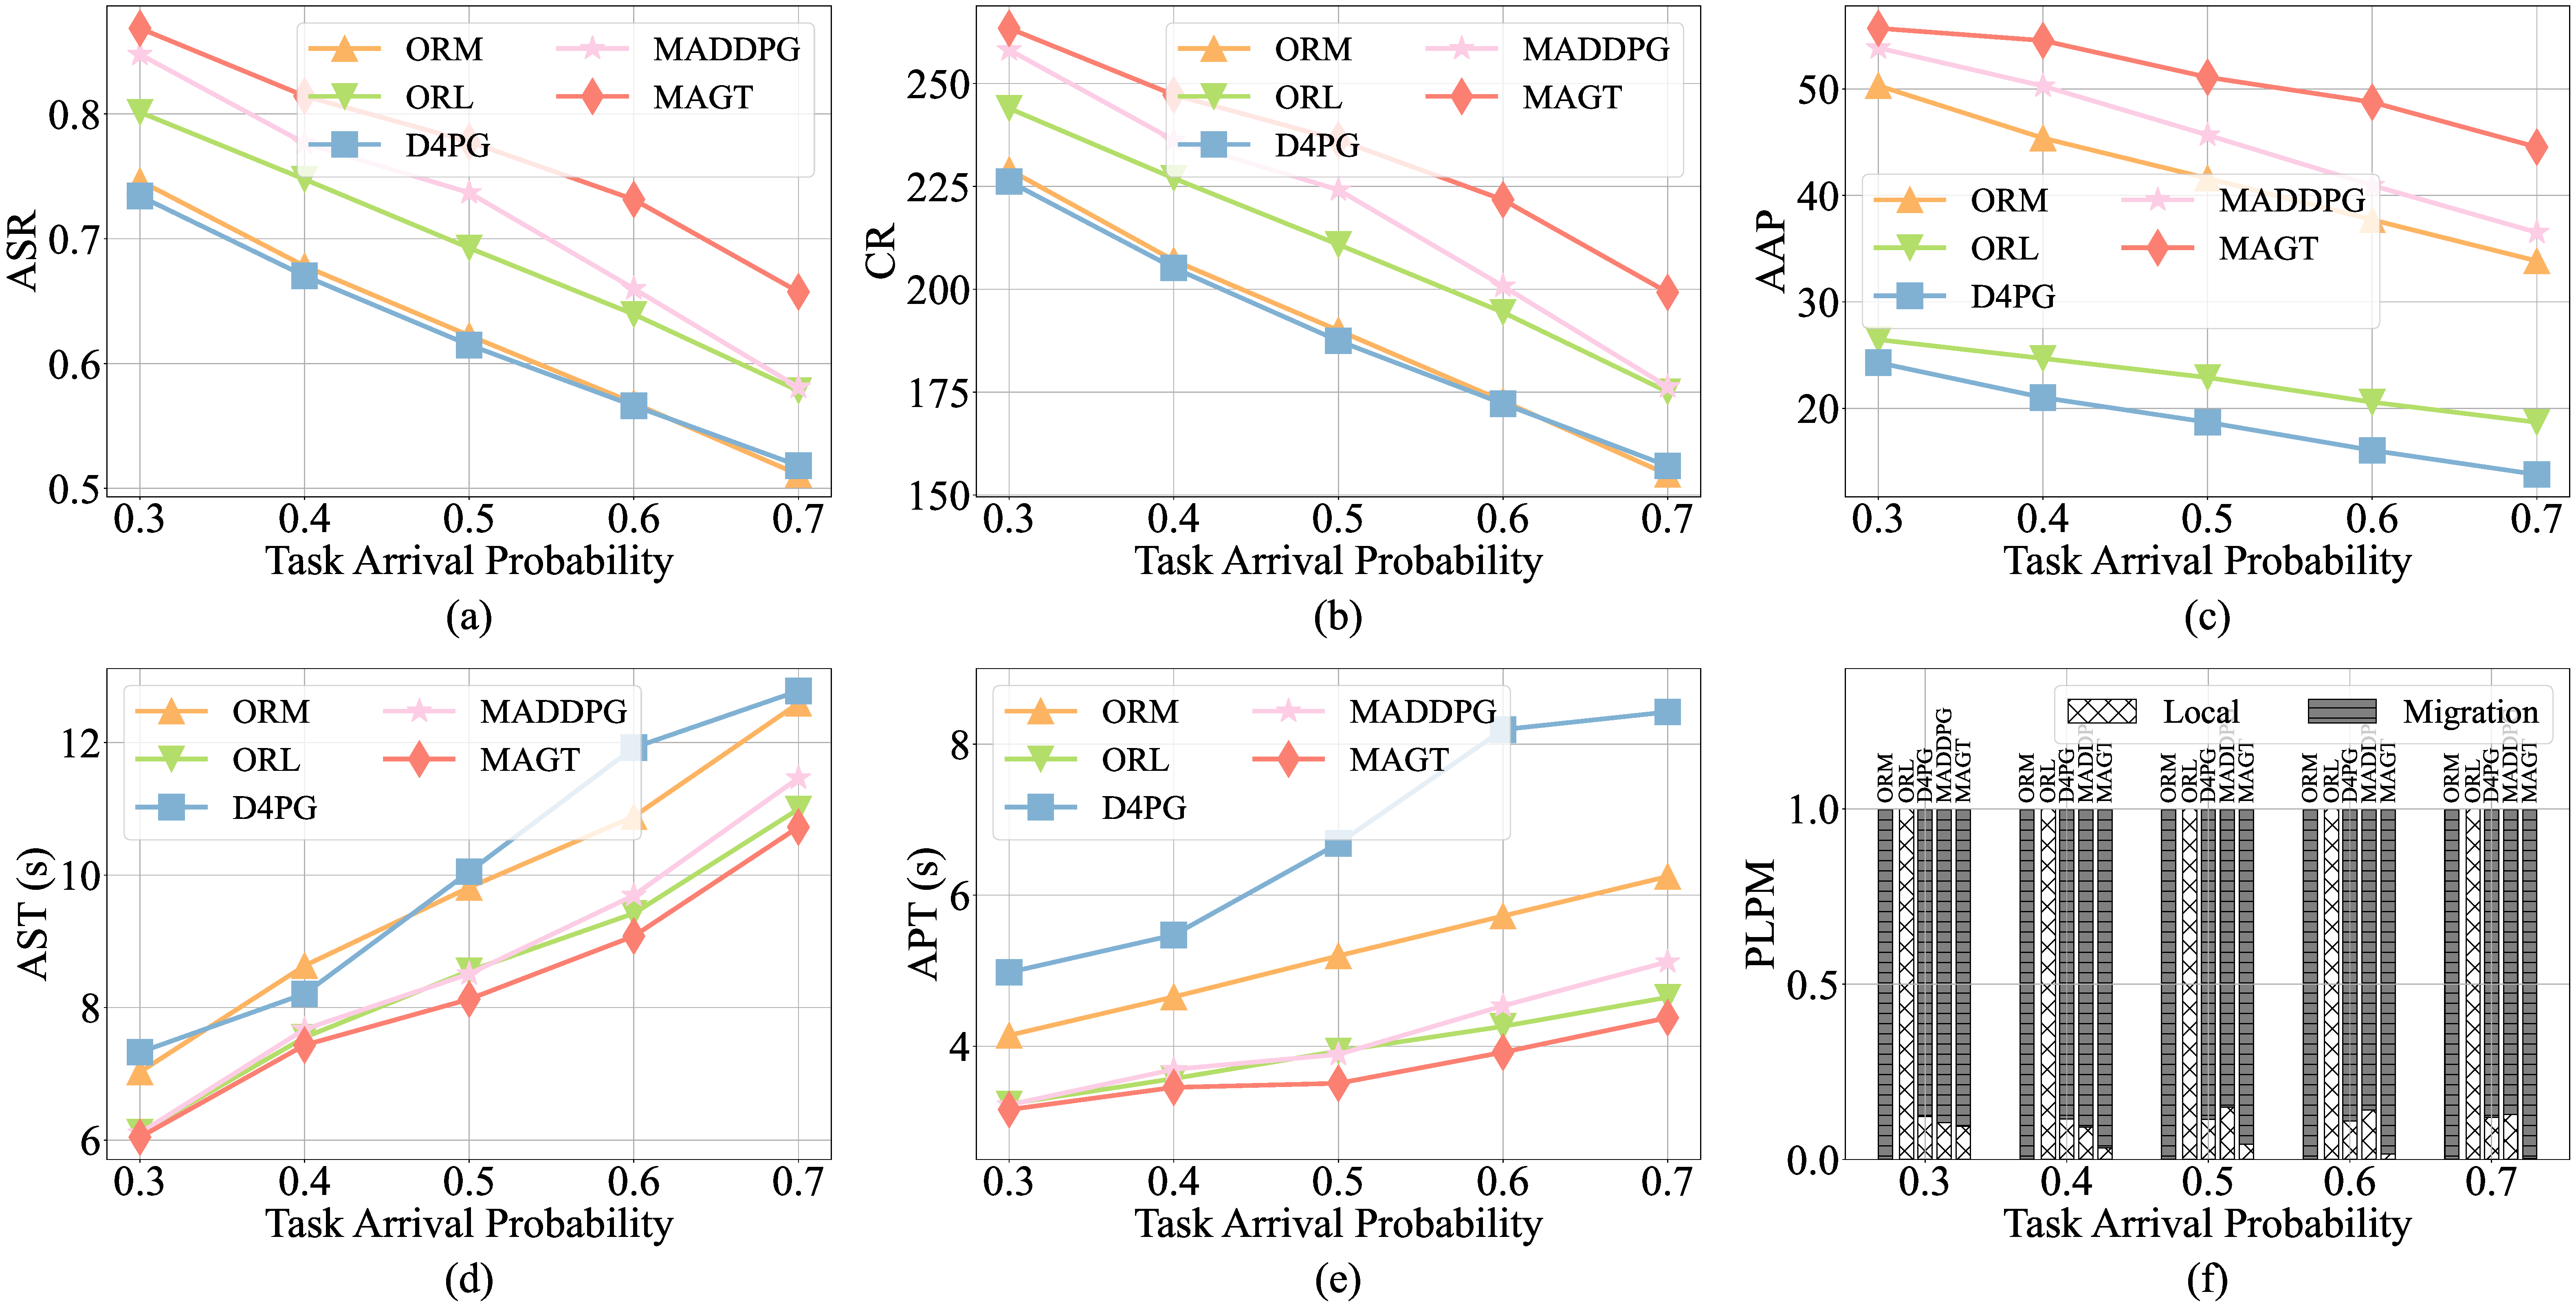
\includegraphics[width=0.9\textwidth]{fig/Fig3-7-different-task-arrival-probability.pdf}
	\end{figure}
\end{textblock*}
\end{center}
}

\only<8-8>{
\frametitle{\englishfont \underline{实验}:任务到达概率的影响}
\begin{center} \englishfont \footnotesize
\begin{textblock*}{\textwidth}(1cm,1.8cm)
	\begin{figure}
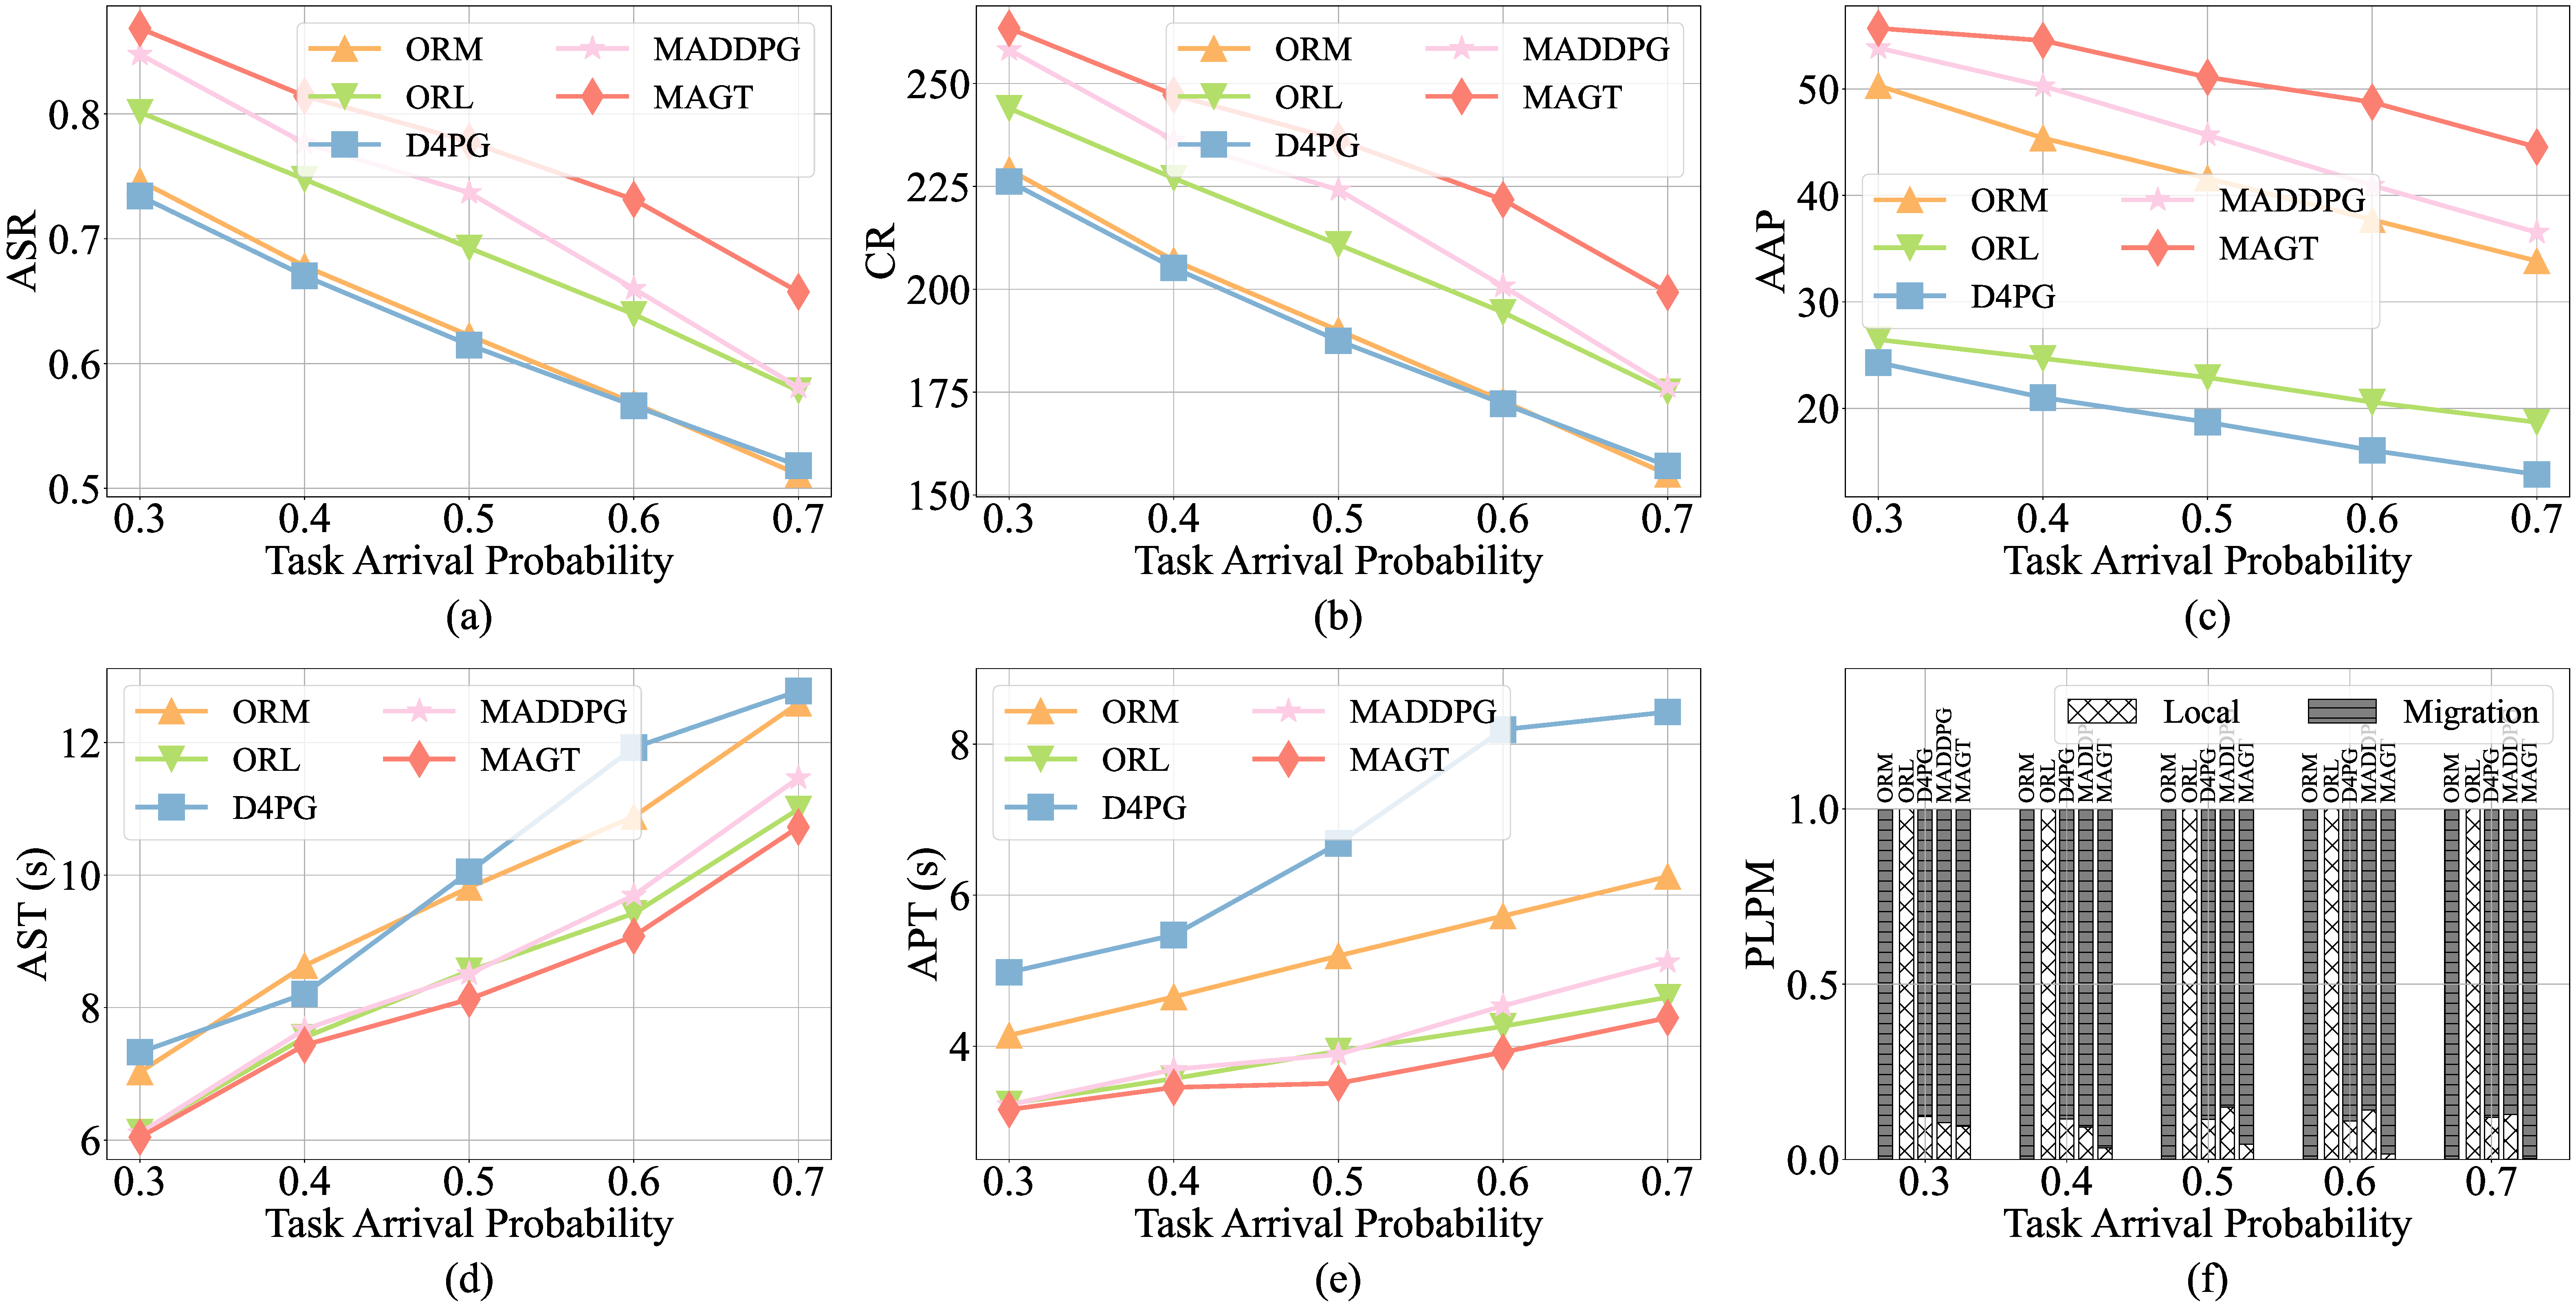
\includegraphics[width=0.9\textwidth]{fig/Fig3-7-different-task-arrival-probability.pdf}
	\end{figure}
\end{textblock*}
\end{center}
}

\only<8-8>{
\begin{center} \englishfont \footnotesize
\begin{textblock*}{\textwidth}(-4.3cm,1.8cm)
{\LARGE{\color{red}\ding{216}}}
\end{textblock*}
\end{center}

\begin{center} \englishfont \footnotesize
\begin{textblock*}{\textwidth}(0cm,1.75cm)
{\LARGE{\color{red}\ding{216}}}
\end{textblock*}
\end{center}

\begin{center} \englishfont \footnotesize
\begin{textblock*}{\textwidth}(5.5cm,1.8cm)
{\LARGE{\color{red}\ding{216}}}
\end{textblock*}
\end{center}

\begin{center} \englishfont \footnotesize
\begin{textblock*}{\textwidth}(0.65cm,6.76cm)
{\LARGE{\color{red}\ding{216}}}
\end{textblock*}
\end{center}

\begin{center} \englishfont \footnotesize
\begin{textblock*}{\textwidth}(-2.7cm,6.2cm)
{\LARGE{\color{red}\ding{216}}}
\end{textblock*}
\end{center}
}
\end{overlayarea}
\end{frame}
\subsection[\englishfont 2.3 面向车载信息物理融合的质量-开销均衡优化]{2.3 面向车载信息物理融合的质量-开销均衡优化}

\begin{frame}{研究贡献}
\newBackground
\begin{center}
\begin{textblock*}{\textwidth}(-2cm,1.8cm)
  \small \englishfont \colorbox{cqublue}{\color{white}{创新的服务质量与系统开销均衡策略是实现}}
\end{textblock*}
\end{center}

\begin{center}
\begin{textblock*}{\textwidth}(-2cm,2.3cm)
  \small \englishfont \colorbox{cqublue}{\color{white}{{\color{yellow}{高质量、低成本和可扩展}}\hspace{0.25em}VCPS的{\color{yellow}{理论保障}}}}
\end{textblock*}
\end{center}

\begin{center}
\begin{textblock*}{\textwidth}(-2.1cm,3.2cm)
\begin{minipage}[t]{0.6\textwidth}
\begin{itemize}[itemsep=0.2\baselineskip] \englishfont 
	\item[\ding{111}] {{\color{cqublue}{\textbf{问题}}}:{\color{red}{双目标优化}}问题}
	\begin{itemize}[itemsep=0.2\baselineskip]
	\begin{small}
		\item[\ding{226}] \underline{最大化}VCPS质量:视图及时性和一致性
		\item[\ding{226}] \underline{最小化}VCPS开销:信息冗余度、感知开销和传输开销
	\end{small}
	\end{itemize}
	\item[\ding{111}] {{\color{cqublue}{\textbf{算法}}}:基于多目标的多智能体深度强化学习算法 ({\color{red}{MAMO}})} 
	\item[\ding{111}] {{\color{cqublue}{\textbf{实验}}}:有效实现质量和开销的均衡} 
\end{itemize}
\end{minipage}
\end{textblock*}
\end{center}


\begin{center}
\begin{textblock*}{\textwidth}(-1.6cm,7.5cm)
\fbox{\begin{minipage}[t]{0.7\textwidth}\englishfont \tiny [5] LIU K,\underline{\textcolor{cqublue}{XU X}}, DAI P, et al. \textcolor{cqublue}{Cooperative sensing and uploading for quality-cost tradeoff of digital twins in VEC}[J]. IEEE Transactions on Consumer Electronics (\textcolor{red}{TCE}), under minor revision. (中科院SCI 2区)
\end{minipage}}
\end{textblock*}
\end{center}

\begin{center}
\begin{textblock*}{\textwidth}(6.2cm,2cm)
\begin{figure}
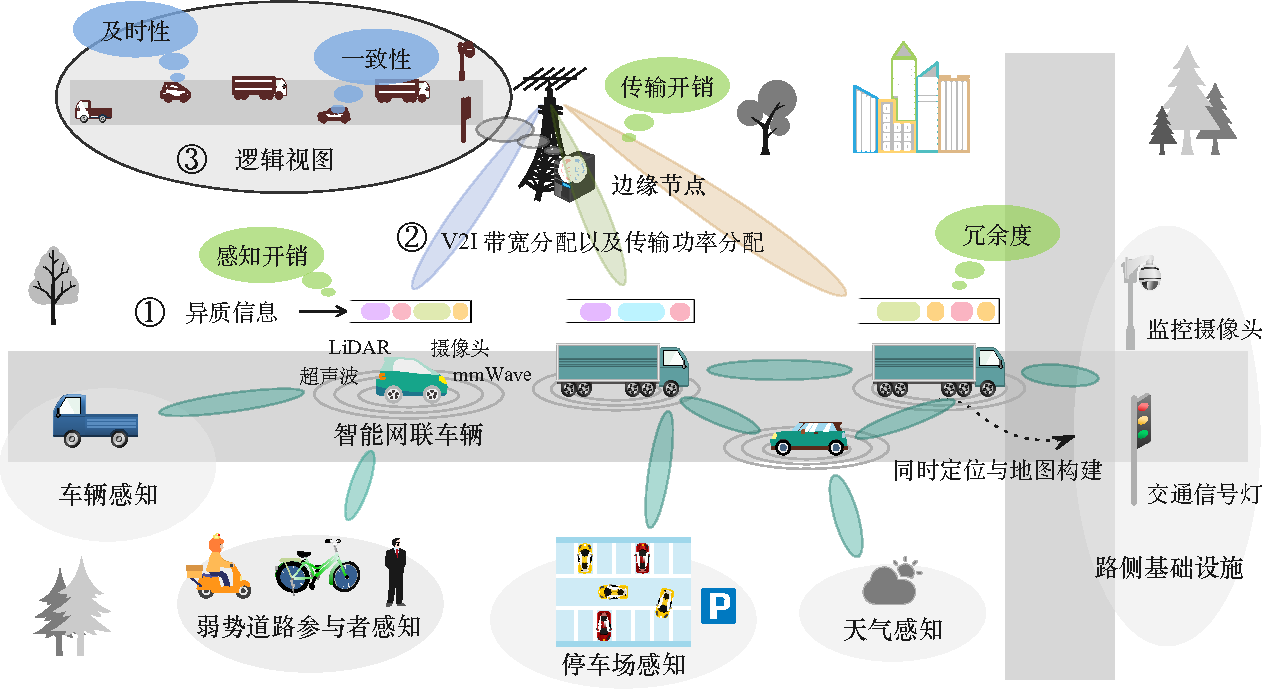
\includegraphics[width=0.38\textwidth]{fig/Fig4-1-architerture.pdf}
\end{figure}
\begin{figure}
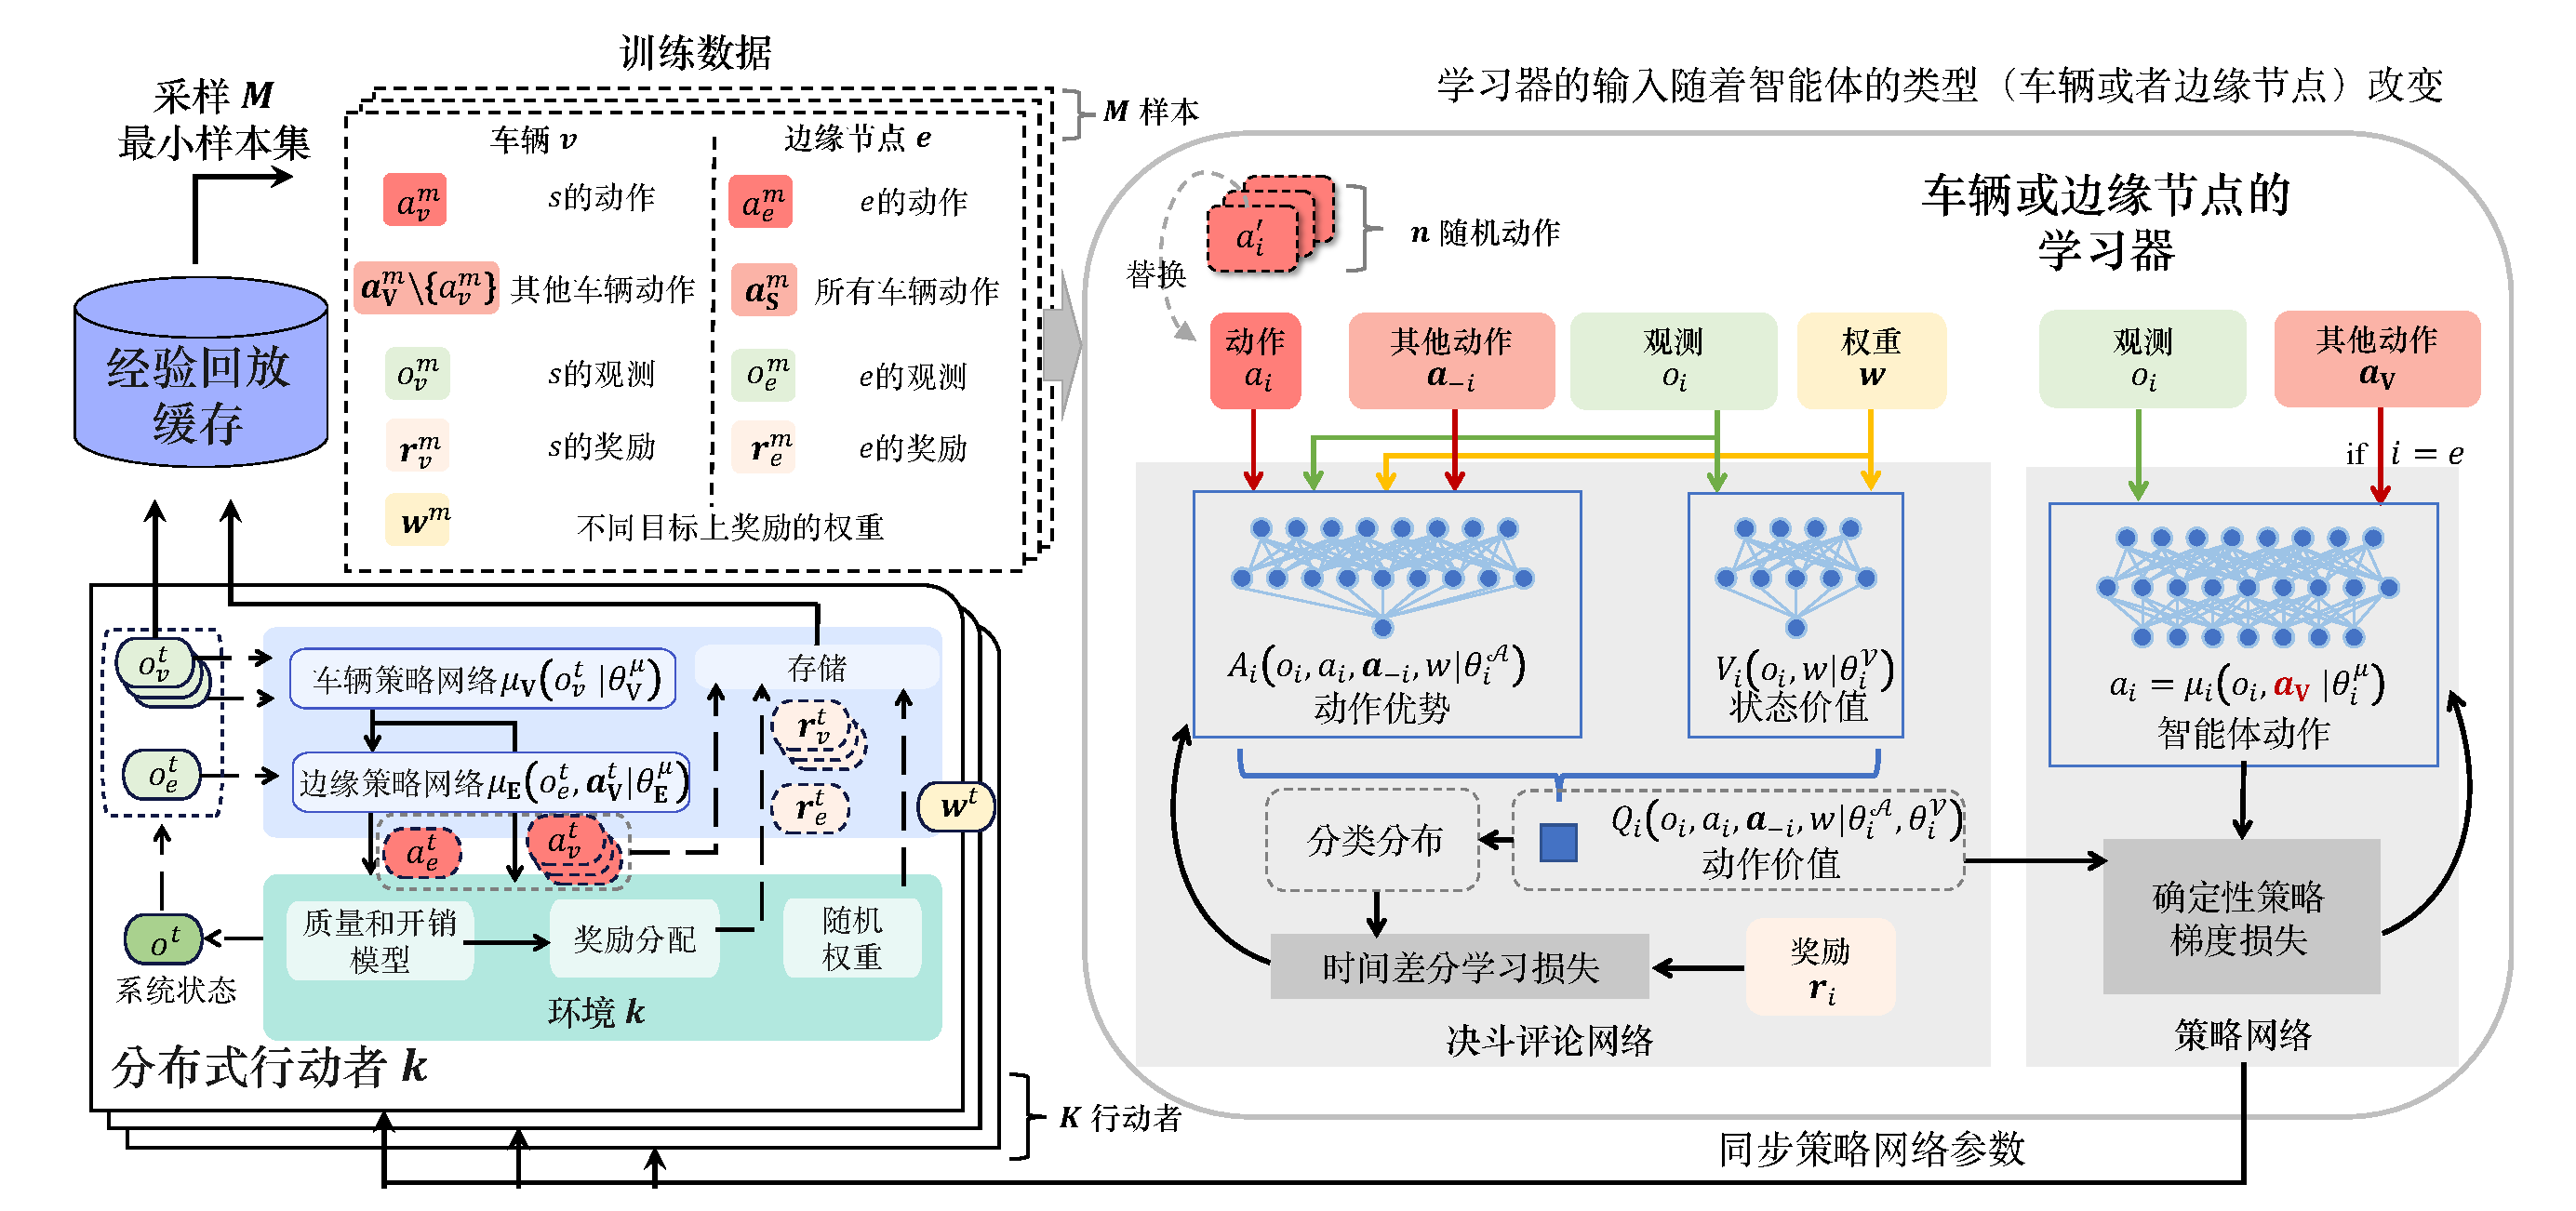
\includegraphics[width=0.38\textwidth]{fig/Fig4-2-solution-model.pdf}
\end{figure}
\end{textblock*}
\end{center}
\end{frame}

\begin{frame}{协同感知与 V2I 上传场景}
\frametitle{\englishfont \underline{问题}:逻辑视图构建场景}
\newBackground
\begin{center}
\begin{textblock*}{\textwidth}(3cm,2cm)
\begin{figure}
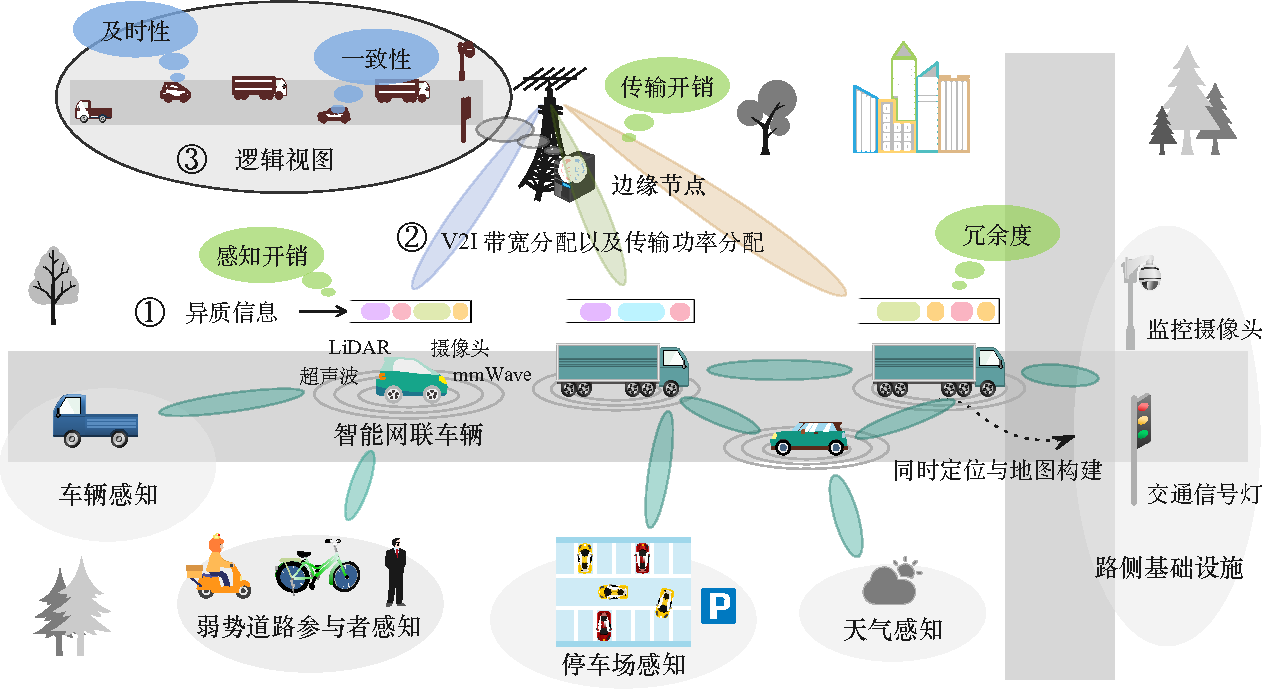
\includegraphics[width=0.75\textwidth]{fig/Fig4-1-architerture.pdf}
\end{figure}
\end{textblock*}
\end{center}

\begin{center}
\begin{textblock*}{\textwidth}(0.5cm,2cm)
\begin{itemize}[itemsep=0.2\baselineskip] \englishfont
		\item[\ding{111}] {\color{cqublue}{视图质量}}
		\begin{itemize}[itemsep=0.2\baselineskip] \small
			\item[\ding{226}] 及时性
			\item[\ding{226}] 一致性
		\end{itemize}
		\item[\ding{111}] {\color{cqublue}{视图开销}}
		\begin{itemize}[itemsep=0.2\baselineskip] \small
			\item[\ding{226}] 感知开销
			\item[\ding{226}] 传输开销
			\item[\ding{226}] 冗余度
		\end{itemize}
\end{itemize}
\end{textblock*}
\end{center}
\end{frame}

\begin{frame}
\newBackground
\frametitle{\englishfont \underline{问题}:VCPS 质量/开销模型}

\begin{overlayarea}{\textwidth}{3cm}
\only<1-1>{
\begin{center}
\begin{textblock*}{0.6\textwidth}(0cm,1.8cm)
\begin{equation}
	\mathscr{Q}=\frac{\sum_{\forall t \in \mathbf{T}} \sum_{\forall e \in \mathbf{E}} \sum_{\forall i \in \mathbf{I}_e^t} \operatorname{QV}_{i}}{\sum_{\forall t \in \mathbf{T}} \sum_{\forall e \in \mathbf{E}} |\mathbf{I}_e^t| } \notag
\end{equation}
\end{textblock*}
\end{center}
}

\only<1-4>{
\begin{center}
\begin{textblock*}{0.6\textwidth}(0cm,4.8cm)
\begin{equation}
	\mathscr{C}=\frac{\sum_{\forall t \in \mathbf{T}} \sum_{\forall e \in \mathbf{E}} \sum_{\forall i \in \mathbf{I}_e^t}  \operatorname{CV}_{i}}{\sum_{\forall t \in \mathbf{T}} \sum_{\forall e \in \mathbf{E}} |\mathbf{I}_e^t| } \notag
\end{equation}
\end{textblock*}
\end{center}
}

\only<2-2>{
\begin{center}
\begin{textblock*}{0.6\textwidth}(0cm,1.8cm)
\begin{equation}
	\mathscr{Q}=\frac{\sum_{\forall t \in \mathbf{T}} \sum_{\forall e \in \mathbf{E}} \sum_{\forall i \in \mathbf{I}_e^t} {\color{red}{\operatorname{QV}_{i}}}}{\sum_{\forall t \in \mathbf{T}} \sum_{\forall e \in \mathbf{E}} |\mathbf{I}_e^t| } \notag
\end{equation}
\end{textblock*}
\end{center}
}

\only<2-2>{
\begin{center}
\begin{textblock*}{0.6\textwidth}(0cm,1.8cm)
\begin{equation}
	\mathscr{Q}=\frac{\sum_{\forall t \in \mathbf{T}} \sum_{\forall e \in \mathbf{E}} \sum_{\forall i \in \mathbf{I}_e^t} {\color{red}{\operatorname{QV}_{i}}}}{\sum_{\forall t \in \mathbf{T}} \sum_{\forall e \in \mathbf{E}} |\mathbf{I}_e^t| } \notag
\end{equation}
\end{textblock*}
\end{center}
}

\only<2-2>{
\begin{center}
\begin{textblock*}{1\textwidth}(4.4cm,1.8cm)
视图质量
\begin{equation}
	{\color{red}{\operatorname{QV}_{i}}}= w_1 (1 -\hat{\Theta_{i}}) + w_2 (1 - \hat{\Psi_{i}}), \forall i \in \mathbf{I}_{e}^t, \forall e \in \mathbf{E} \notag
\end{equation}
\end{textblock*}
\end{center}
}

\only<3->{
\begin{center}
\begin{textblock*}{0.6\textwidth}(0cm,1.8cm)
\begin{equation}
	\mathscr{Q}=\frac{\sum_{\forall t \in \mathbf{T}} \sum_{\forall e \in \mathbf{E}} \sum_{\forall i \in \mathbf{I}_e^t} \operatorname{QV}_{i}}{\sum_{\forall t \in \mathbf{T}} \sum_{\forall e \in \mathbf{E}} |\mathbf{I}_e^t| } \notag
\end{equation}
\end{textblock*}
\end{center}
}

\only<3-3>{
\begin{center}
\begin{textblock*}{1\textwidth}(4.4cm,1.8cm)
视图质量
\begin{equation}
	\operatorname{QV}_{i}= w_1 (1 -{\color{red}{\hat{\Theta_{i}}}}) + w_2 (1 - \hat{\Psi_{i}}), \forall i \in \mathbf{I}_{e}^t, \forall e \in \mathbf{E} \notag
\end{equation}
\end{textblock*}
\end{center}
}

\only<3-3>{
\begin{center}
\begin{textblock*}{1\textwidth}(2.4cm,3.4cm)
{\color{red}{$\hat{\Theta_{i}}$}}:视图及时性
\end{textblock*}
\end{center}
}

\only<4->{
\begin{center}
\begin{textblock*}{1\textwidth}(2.4cm,3.4cm)
$\hat{\Theta_{i}}$:视图及时性
\end{textblock*}
\end{center}
}

\only<4-4>{
\begin{center}
\begin{textblock*}{1\textwidth}(4.4cm,1.8cm)
视图质量
\begin{equation}
	\operatorname{QV}_{i}= w_1 (1 -\hat{\Theta_{i}}) + w_2 (1 - {\color{red}{\hat{\Psi_{i}}}}), \forall i \in \mathbf{I}_{e}^t, \forall e \in \mathbf{E} \notag
\end{equation}
\end{textblock*}
\end{center}
}

\only<4-4>{
\begin{center}
\begin{textblock*}{1\textwidth}(6.4cm,3.4cm)
{\color{red}{$\hat{\Psi_{i}}$}}:视图一致性
\end{textblock*}
\end{center}
}

\only<5->{
\begin{center}
\begin{textblock*}{1\textwidth}(4.4cm,1.8cm)
视图质量
\begin{equation}
	\operatorname{QV}_{i}= w_1 (1 -\hat{\Theta_{i}}) + w_2 (1 - \hat{\Psi_{i}}), \forall i \in \mathbf{I}_{e}^t, \forall e \in \mathbf{E} \notag
\end{equation}
\end{textblock*}
\end{center}
}

\only<5->{
\begin{center}
\begin{textblock*}{1\textwidth}(6.4cm,3.4cm)
$\hat{\Psi_{i}}$:视图一致性
\end{textblock*}
\end{center}
}

\only<5-5>{
\begin{center}
\begin{textblock*}{0.6\textwidth}(0cm,4.8cm)
\begin{equation}
	\mathscr{C}=\frac{\sum_{\forall t \in \mathbf{T}} \sum_{\forall e \in \mathbf{E}} \sum_{\forall i \in \mathbf{I}_e^t}  {\color{red}{\operatorname{CV}_{i}}}}{\sum_{\forall t \in \mathbf{T}} \sum_{\forall e \in \mathbf{E}} |\mathbf{I}_e^t| } \notag
\end{equation}
\end{textblock*}
\end{center}
}

\only<5-5>{
\begin{center}
\begin{textblock*}{1\textwidth}(4.4cm,4.8cm)
视图开销
\begin{equation}
	{\color{red}{\operatorname{CV}_{i}}} = w_3  \hat{\Xi_{i}} +  w_4 \hat{\Phi_{i}} + w_5 \hat{\Omega_{i}}, \forall i \in \mathbf{I}_{e}^t, \forall e \in \mathbf{E} \notag
\end{equation}
\end{textblock*}
\end{center}
}

\only<6->{
\begin{center}
\begin{textblock*}{0.6\textwidth}(0cm,4.8cm)
\begin{equation}
	\mathscr{C}=\frac{\sum_{\forall t \in \mathbf{T}} \sum_{\forall e \in \mathbf{E}} \sum_{\forall i \in \mathbf{I}_e^t}  \operatorname{CV}_{i}}{\sum_{\forall t \in \mathbf{T}} \sum_{\forall e \in \mathbf{E}} |\mathbf{I}_e^t| } \notag
\end{equation}
\end{textblock*}
\end{center}
}

\only<6-6>{
\begin{center}
\begin{textblock*}{1\textwidth}(4.4cm,4.8cm)
视图开销
\begin{equation}
	\operatorname{CV}_{i} = w_3  {\color{red}{\hat{\Xi_{i}}}} +  w_4 \hat{\Phi_{i}} + w_5 \hat{\Omega_{i}}, \forall i \in \mathbf{I}_{e}^t, \forall e \in \mathbf{E} \notag
\end{equation}
\end{textblock*}
\end{center}
}

\only<6-6>{
\begin{center}
\begin{textblock*}{1\textwidth}(2.4cm,6.4cm)
{\color{red}{$\hat{\Xi_{i}}$}}:视图冗余度
\end{textblock*}
\end{center}
}

\only<7->{
\begin{center}
\begin{textblock*}{1\textwidth}(2.4cm,6.4cm)
$\hat{\Xi_{i}}$:视图冗余度
\end{textblock*}
\end{center}
}

\only<7-7>{
\begin{center}
\begin{textblock*}{1\textwidth}(4.4cm,4.8cm)
视图开销
\begin{equation}
	\operatorname{CV}_{i} = w_3 \hat{\Xi_{i}} +  w_4 {\color{red}{\hat{\Phi_{i}}}} + w_5 \hat{\Omega_{i}}, \forall i \in \mathbf{I}_{e}^t, \forall e \in \mathbf{E} \notag
\end{equation}
\end{textblock*}
\end{center}
}

\only<7-7>{
\begin{center}
\begin{textblock*}{1\textwidth}(6.4cm,6.4cm)
{\color{red}{$\hat{\Phi_{i}}$}}:视图感知开销
\end{textblock*}
\end{center}
}

\only<8->{
\begin{center}
\begin{textblock*}{1\textwidth}(6.4cm,6.4cm)
$\hat{\Phi_{i}}$:视图感知开销
\end{textblock*}
\end{center}
}

\only<8-8>{
\begin{center}
\begin{textblock*}{1\textwidth}(4.4cm,4.8cm)
视图开销
\begin{equation}
	\operatorname{CV}_{i} = w_3 \hat{\Xi_{i}} +  w_4 \hat{\Phi_{i}} + w_5 {\color{red}{\hat{\Omega_{i}}}}, \forall i \in \mathbf{I}_{e}^t, \forall e \in \mathbf{E} \notag
\end{equation}
\end{textblock*}
\end{center}
}

\only<8-8>{
\begin{center}
\begin{textblock*}{1\textwidth}(4.4cm,7.4cm)
{\color{red}{$\hat{\Omega_{i}}$}}:视图传输开销
\end{textblock*}
\end{center}
}

\end{overlayarea}

\begin{center}
\begin{textblock*}{0.6\textwidth}(1cm,1.8cm)
\begin{itemize} \englishfont
	\item[\ding{111}]  {\color{cqublue}{VCPS 质量模型}}
	\item
	\item
	\item
	\item
	\item[\ding{111}]  {\color{cqublue}{VCPS开销模型}}
\end{itemize}
\end{textblock*}
\end{center}

\end{frame}

\begin{frame}
\frametitle{\englishfont \underline{问题}:双目标优化问题}
\newBackground

\begin{overlayarea}{\textwidth}{3cm}
\only<1-1>{
\begin{center}
\begin{textblock*}{1\textwidth}(0.5cm,1.6cm)
\begin{align}
	\mathcal{P}4.1: & \max_{\mathbf{C}, \boldsymbol{\Lambda}, \mathbf{P}, \boldsymbol{\Pi}, \mathbf{B}} \mathscr{Q}, \min_{\mathbf{C}, \boldsymbol{\Lambda}, \mathbf{P}, \boldsymbol{\Pi}, \mathbf{B}} \mathscr{C} \notag \\
	\text { s.t. }
	& (4.1) \sim (4.5) \notag \\
    &\mathcal{C}4.1: \sum_{\forall d \subseteq \mathbf{D}_v^t} \lambda_{d, v}^{t} \mu_d<1,\ \forall v \in \mathbf{V}, \forall t \in \mathbf{T} \notag \\
    &\mathcal{C}4.2: \inf_{\mathbb{P} \in \tilde{p}} \operatorname{Pr}_{[\mathbb{P}]}\left(\operatorname{SNR}_{v, e}^{t} \geq \operatorname{SNR}_{v, e}^{\operatorname{tgt}}\right) \geq \delta, \forall v \in \mathbf{V}, \forall t \in \mathbf{T} \notag \\
    &\mathcal{C}4.3: {\sum_{\forall v \in \mathbf{V}_e^{t}}b_v^t} \leq b_e, \forall t \in \mathbf{T} \notag
\end{align}
\end{textblock*}
\end{center}
}

\only<2-2>{
\begin{center}
\begin{textblock*}{1\textwidth}(0.5cm,1.6cm)
\begin{align}
	\mathcal{P}4.2: & \max_{ \mathbf{C}, \boldsymbol{\Lambda}, \mathbf{P}, \boldsymbol{\Pi}, \mathbf{B} } \left (\mathscr{Q}, {\color{red}{\mathscr{P}}} \right )  \notag \\
	\text { s.t. }
	& (4.1) \sim (4.5) \notag \\
    &\mathcal{C}4.1: \sum_{\forall d \subseteq \mathbf{D}_v^t} \lambda_{d, v}^{t} \mu_d<1,\ \forall v \in \mathbf{V}, \forall t \in \mathbf{T} \notag \\
    &\mathcal{C}4.2: \inf_{\mathbb{P} \in \tilde{p}} \operatorname{Pr}_{[\mathbb{P}]}\left(\operatorname{SNR}_{v, e}^{t} \geq \operatorname{SNR}_{v, e}^{\operatorname{tgt}}\right) \geq \delta, \forall v \in \mathbf{V}, \forall t \in \mathbf{T} \notag \\
    &\mathcal{C}4.3: {\sum_{\forall v \in \mathbf{V}_e^{t}}b_v^t} \leq b_e, \forall t \in \mathbf{T} \notag
\end{align}
\end{textblock*}
\end{center}
}

\only<2-2>{
\begin{center}
\begin{textblock*}{1\textwidth}(0.5cm,7.1cm) \englishfont
{\color{red}{$\mathscr{P}$}}:VCPS 利润 $\mathscr{P}= \frac{\sum_{\forall t \in \mathbf{T}} \sum_{\forall e \in \mathbf{E}} \sum_{\forall i \in \mathbf{I}_e^t}   \operatorname{PV}_{j} }{\sum_{\forall t \in \mathbf{T}} \sum_{\forall e \in \mathbf{E}} |\mathbf{I}_e^t| }$
\end{textblock*}
\end{center}
}


\only<3-3>{
\begin{center}
\begin{textblock*}{1\textwidth}(0.5cm,1.6cm)
\begin{align}
	\mathcal{P}4.2: & \max_{ {\color{red}{\mathbf{C}}}, \boldsymbol{\Lambda}, \mathbf{P}, \boldsymbol{\Pi}, \mathbf{B} } \left (\mathscr{Q}, \mathscr{P} \right )  \notag \\
	\text { s.t. }
	& (4.1) \sim (4.5) \notag \\
    &\mathcal{C}4.1: \sum_{\forall d \subseteq \mathbf{D}_v^t} \lambda_{d, v}^{t} \mu_d<1,\ \forall v \in \mathbf{V}, \forall t \in \mathbf{T} \notag \\
    &\mathcal{C}4.2: \inf_{\mathbb{P} \in \tilde{p}} \operatorname{Pr}_{[\mathbb{P}]}\left(\operatorname{SNR}_{v, e}^{t} \geq \operatorname{SNR}_{v, e}^{\operatorname{tgt}}\right) \geq \delta, \forall v \in \mathbf{V}, \forall t \in \mathbf{T} \notag \\
    &\mathcal{C}4.3: {\sum_{\forall v \in \mathbf{V}_e^{t}}b_v^t} \leq b_e, \forall t \in \mathbf{T} \notag
\end{align}
\end{textblock*}
\end{center}
}

\only<3-3>{
\begin{center}
\begin{textblock*}{1\textwidth}(0.5cm,7.1cm) \englishfont
{\color{red}{$\mathbf{C}$}}:感知信息决策 $\mathbf{C} = \left \{ c_{d, v}^t \vert \forall d \in \mathbf{D}_{v}, \forall v \in \mathbf{V}, \forall t \in \mathbf{T} \right  \}$
\end{textblock*}
\end{center}
}

\only<4-4>{
\begin{center}
\begin{textblock*}{1\textwidth}(0.5cm,1.6cm)
\begin{align}
	\mathcal{P}4.2: & \max_{ \mathbf{C}, {\color{red}{\boldsymbol{\Lambda}}}, \mathbf{P}, \boldsymbol{\Pi}, \mathbf{B} } \left (\mathscr{Q}, \mathscr{P} \right )  \notag \\
	\text { s.t. }
	& (4.1) \sim (4.5) \notag \\
    &\mathcal{C}4.1: \sum_{\forall d \subseteq \mathbf{D}_v^t} \lambda_{d, v}^{t} \mu_d<1,\ \forall v \in \mathbf{V}, \forall t \in \mathbf{T} \notag \\
    &\mathcal{C}4.2: \inf_{\mathbb{P} \in \tilde{p}} \operatorname{Pr}_{[\mathbb{P}]}\left(\operatorname{SNR}_{v, e}^{t} \geq \operatorname{SNR}_{v, e}^{\operatorname{tgt}}\right) \geq \delta, \forall v \in \mathbf{V}, \forall t \in \mathbf{T} \notag \\
    &\mathcal{C}4.3: {\sum_{\forall v \in \mathbf{V}_e^{t}}b_v^t} \leq b_e, \forall t \in \mathbf{T} \notag
\end{align}
\end{textblock*}
\end{center}
}

\only<4-4>{
\begin{center}
\begin{textblock*}{1\textwidth}(0.5cm,7.1cm) \englishfont
{\color{red}{$\boldsymbol{\Lambda}$}}:感知频率 $\boldsymbol{\Lambda} = \left \{ \lambda_{d, v}^{t} \vert \forall d \in \mathbf{D}_v^t  , \forall v \in \mathbf{V}, \forall t \in \mathbf{T} \right \}$
\end{textblock*}
\end{center}
}

\only<5-5>{
\begin{center}
\begin{textblock*}{1\textwidth}(0.5cm,1.6cm)
\begin{align}
	\mathcal{P}4.2: & \max_{ \mathbf{C}, \boldsymbol{\Lambda}, {\color{red}{\mathbf{P}}}, \boldsymbol{\Pi}, \mathbf{B} } \left (\mathscr{Q}, \mathscr{P} \right )  \notag \\
	\text { s.t. }
	& (4.1) \sim (4.5) \notag \\
    &\mathcal{C}4.1: \sum_{\forall d \subseteq \mathbf{D}_v^t} \lambda_{d, v}^{t} \mu_d<1,\ \forall v \in \mathbf{V}, \forall t \in \mathbf{T} \notag \\
    &\mathcal{C}4.2: \inf_{\mathbb{P} \in \tilde{p}} \operatorname{Pr}_{[\mathbb{P}]}\left(\operatorname{SNR}_{v, e}^{t} \geq \operatorname{SNR}_{v, e}^{\operatorname{tgt}}\right) \geq \delta, \forall v \in \mathbf{V}, \forall t \in \mathbf{T} \notag \\
    &\mathcal{C}4.3: {\sum_{\forall v \in \mathbf{V}_e^{t}}b_v^t} \leq b_e, \forall t \in \mathbf{T} \notag
\end{align}
\end{textblock*}
\end{center}
}

\only<5-5>{
\begin{center}
\begin{textblock*}{1\textwidth}(0.5cm,7.1cm) \englishfont
{\color{red}{$\mathbf{P}$}}:上传优先级 $\mathbf{P} = \left \{ p_{d, v}^{t} \vert \forall d \in \mathbf{D}_v^t  , \forall v \in \mathbf{V}, \forall t \in \mathbf{T}\right \}$
\end{textblock*}
\end{center}
}

\only<6-6>{
\begin{center}
\begin{textblock*}{1\textwidth}(0.5cm,1.6cm)
\begin{align}
	\mathcal{P}4.2: & \max_{ \mathbf{C}, \boldsymbol{\Lambda}, \mathbf{P}, {\color{red}{\boldsymbol{\Pi}}}, \mathbf{B} } \left (\mathscr{Q}, \mathscr{P} \right )  \notag \\
	\text { s.t. }
	& (4.1) \sim (4.5) \notag \\
    &\mathcal{C}4.1: \sum_{\forall d \subseteq \mathbf{D}_v^t} \lambda_{d, v}^{t} \mu_d<1,\ \forall v \in \mathbf{V}, \forall t \in \mathbf{T} \notag \\
    &\mathcal{C}4.2: \inf_{\mathbb{P} \in \tilde{p}} \operatorname{Pr}_{[\mathbb{P}]}\left(\operatorname{SNR}_{v, e}^{t} \geq \operatorname{SNR}_{v, e}^{\operatorname{tgt}}\right) \geq \delta, \forall v \in \mathbf{V}, \forall t \in \mathbf{T} \notag \\
    &\mathcal{C}4.3: {\sum_{\forall v \in \mathbf{V}_e^{t}}b_v^t} \leq b_e, \forall t \in \mathbf{T} \notag
\end{align}
\end{textblock*}
\end{center}
}

\only<6-6>{
\begin{center}
\begin{textblock*}{1\textwidth}(0.5cm,7.1cm) \englishfont
{\color{red}{$\boldsymbol{\Pi}$}}:传输功率 $\boldsymbol{\Pi} = \left \{ \pi_v^t \vert \forall v \in \mathbf{V}, \forall t \in \mathbf{T} \right \}$
\end{textblock*}
\end{center}
}

\only<7-7>{
\begin{center}
\begin{textblock*}{1\textwidth}(0.5cm,1.6cm)
\begin{align}
	\mathcal{P}4.2: & \max_{ \mathbf{C}, \boldsymbol{\Lambda}, \mathbf{P}, \boldsymbol{\Pi}, {\color{red}{\mathbf{B}}} } \left (\mathscr{Q}, \mathscr{P} \right )  \notag \\
	\text { s.t. }
	& (4.1) \sim (4.5) \notag \\
    &\mathcal{C}4.1: \sum_{\forall d \subseteq \mathbf{D}_v^t} \lambda_{d, v}^{t} \mu_d<1,\ \forall v \in \mathbf{V}, \forall t \in \mathbf{T} \notag \\
    &\mathcal{C}4.2: \inf_{\mathbb{P} \in \tilde{p}} \operatorname{Pr}_{[\mathbb{P}]}\left(\operatorname{SNR}_{v, e}^{t} \geq \operatorname{SNR}_{v, e}^{\operatorname{tgt}}\right) \geq \delta, \forall v \in \mathbf{V}, \forall t \in \mathbf{T} \notag \\
    &\mathcal{C}4.3: {\sum_{\forall v \in \mathbf{V}_e^{t}}b_v^t} \leq b_e, \forall t \in \mathbf{T} \notag
\end{align}
\end{textblock*}
\end{center}
}

\only<7-7>{
\begin{center}
\begin{textblock*}{1\textwidth}(0.5cm,7.1cm) \englishfont
{\color{red}{$\mathbf{B}$}}:V2I带宽分配 $\mathbf{B} = \left \{ b_v^t \vert \forall v \in \mathbf{V}, \forall t \in \mathbf{T}\right \}$
\end{textblock*}
\end{center}
}

\only<8-8>{
\begin{center}
\begin{textblock*}{1\textwidth}(0.5cm,1.6cm)
\begin{align}
	\mathcal{P}4.2: & \max_{ \mathbf{C}, \boldsymbol{\Lambda}, \mathbf{P}, \boldsymbol{\Pi}, \mathbf{B} } \left (\mathscr{Q}, \mathscr{P} \right )  \notag \\
	\text { s.t. }
	& {\color{red}{(4.1) \sim (4.5)}} \notag \\
    &\mathcal{C}4.1: \sum_{\forall d \subseteq \mathbf{D}_v^t} \lambda_{d, v}^{t} \mu_d<1,\ \forall v \in \mathbf{V}, \forall t \in \mathbf{T} \notag \\
    &\mathcal{C}4.2: \inf_{\mathbb{P} \in \tilde{p}} \operatorname{Pr}_{[\mathbb{P}]}\left(\operatorname{SNR}_{v, e}^{t} \geq \operatorname{SNR}_{v, e}^{\operatorname{tgt}}\right) \geq \delta, \forall v \in \mathbf{V}, \forall t \in \mathbf{T} \notag \\
    &\mathcal{C}4.3: {\sum_{\forall v \in \mathbf{V}_e^{t}}b_v^t} \leq b_e, \forall t \in \mathbf{T} \notag
\end{align}
\end{textblock*}
\end{center}
}

\only<8-8>{
\begin{center}
\begin{textblock*}{1\textwidth}(0.5cm,7.1cm) \englishfont
{\color{red}{$(4.1) \sim (4.5)$}}:决策变量取值范围限制
\end{textblock*}
\end{center}
}

\only<9-9>{
\begin{center}
\begin{textblock*}{1\textwidth}(0.5cm,1.6cm)
\begin{align}
	\mathcal{P}4.2: & \max_{ \mathbf{C}, \boldsymbol{\Lambda}, \mathbf{P}, \boldsymbol{\Pi}, \mathbf{B} } \left (\mathscr{Q}, \mathscr{P} \right )  \notag \\
	\text { s.t. }
	& (4.1) \sim (4.5) \notag \\
    &{\color{red}{\mathcal{C}4.1}}: \sum_{\forall d \subseteq \mathbf{D}_v^t} \lambda_{d, v}^{t} \mu_d<1,\ \forall v \in \mathbf{V}, \forall t \in \mathbf{T} \notag \\
    &\mathcal{C}4.2: \inf_{\mathbb{P} \in \tilde{p}} \operatorname{Pr}_{[\mathbb{P}]}\left(\operatorname{SNR}_{v, e}^{t} \geq \operatorname{SNR}_{v, e}^{\operatorname{tgt}}\right) \geq \delta, \forall v \in \mathbf{V}, \forall t \in \mathbf{T} \notag \\
    &\mathcal{C}4.3: {\sum_{\forall v \in \mathbf{V}_e^{t}}b_v^t} \leq b_e, \forall t \in \mathbf{T} \notag
\end{align}
\end{textblock*}
\end{center}
}

\only<9-9>{
\begin{center}
\begin{textblock*}{1\textwidth}(0.5cm,7.1cm) \englishfont
{\color{red}{$\mathcal{C}4.1$}}:保证队列稳定状态
\end{textblock*}
\end{center}
}

\only<10-10>{
\begin{center}
\begin{textblock*}{1\textwidth}(0.5cm,1.6cm)
\begin{align}
	\mathcal{P}4.2: & \max_{ \mathbf{C}, \boldsymbol{\Lambda}, \mathbf{P}, \boldsymbol{\Pi}, \mathbf{B} } \left (\mathscr{Q}, \mathscr{P} \right )  \notag \\
	\text { s.t. }
	& (4.1) \sim (4.5) \notag \\
    &\mathcal{C}4.1: \sum_{\forall d \subseteq \mathbf{D}_v^t} \lambda_{d, v}^{t} \mu_d<1,\ \forall v \in \mathbf{V}, \forall t \in \mathbf{T} \notag \\
    &{\color{red}{\mathcal{C}4.2}}: \inf_{\mathbb{P} \in \tilde{p}} \operatorname{Pr}_{[\mathbb{P}]}\left(\operatorname{SNR}_{v, e}^{t} \geq \operatorname{SNR}_{v, e}^{\operatorname{tgt}}\right) \geq \delta, \forall v \in \mathbf{V}, \forall t \in \mathbf{T} \notag \\
    &\mathcal{C}4.3: {\sum_{\forall v \in \mathbf{V}_e^{t}}b_v^t} \leq b_e, \forall t \in \mathbf{T} \notag
\end{align}
\end{textblock*}
\end{center}
}

\only<10-10>{
\begin{center}
\begin{textblock*}{1\textwidth}(0.5cm,7.1cm) \englishfont
{\color{red}{$\mathcal{C}4.2$}}:保证传输可靠性
\end{textblock*}
\end{center}
}

\only<11-11>{
\begin{center}
\begin{textblock*}{1\textwidth}(0.5cm,1.6cm)
\begin{align}
	\mathcal{P}4.2: & \max_{ \mathbf{C}, \boldsymbol{\Lambda}, \mathbf{P}, \boldsymbol{\Pi}, \mathbf{B} } \left (\mathscr{Q}, \mathscr{P} \right )  \notag \\
	\text { s.t. }
	& (4.1) \sim (4.5) \notag \\
    &\mathcal{C}4.1: \sum_{\forall d \subseteq \mathbf{D}_v^t} \lambda_{d, v}^{t} \mu_d<1,\ \forall v \in \mathbf{V}, \forall t \in \mathbf{T} \notag \\
    &\mathcal{C}4.2: \inf_{\mathbb{P} \in \tilde{p}} \operatorname{Pr}_{[\mathbb{P}]}\left(\operatorname{SNR}_{v, e}^{t} \geq \operatorname{SNR}_{v, e}^{\operatorname{tgt}}\right) \geq \delta, \forall v \in \mathbf{V}, \forall t \in \mathbf{T} \notag \\
    &{\color{red}{\mathcal{C}4.3}}: {\sum_{\forall v \in \mathbf{V}_e^{t}}b_v^t} \leq b_e, \forall t \in \mathbf{T} \notag
\end{align}
\end{textblock*}
\end{center}
}

\only<11-11>{
\begin{center}
\begin{textblock*}{1\textwidth}(0.5cm,7.1cm) \englishfont
{\color{red}{$\mathcal{C}4.3$}}:边缘节点$e$分配的V2I带宽之和不能超过其容量$b_e$
\end{textblock*}
\end{center}
}

\end{overlayarea}
\end{frame}


\begin{frame}
\frametitle{\englishfont \underline{算法}:流程}
\newBackground
\begin{center}
\begin{textblock*}{\textwidth}(4.5cm,2.6cm)
\begin{figure}
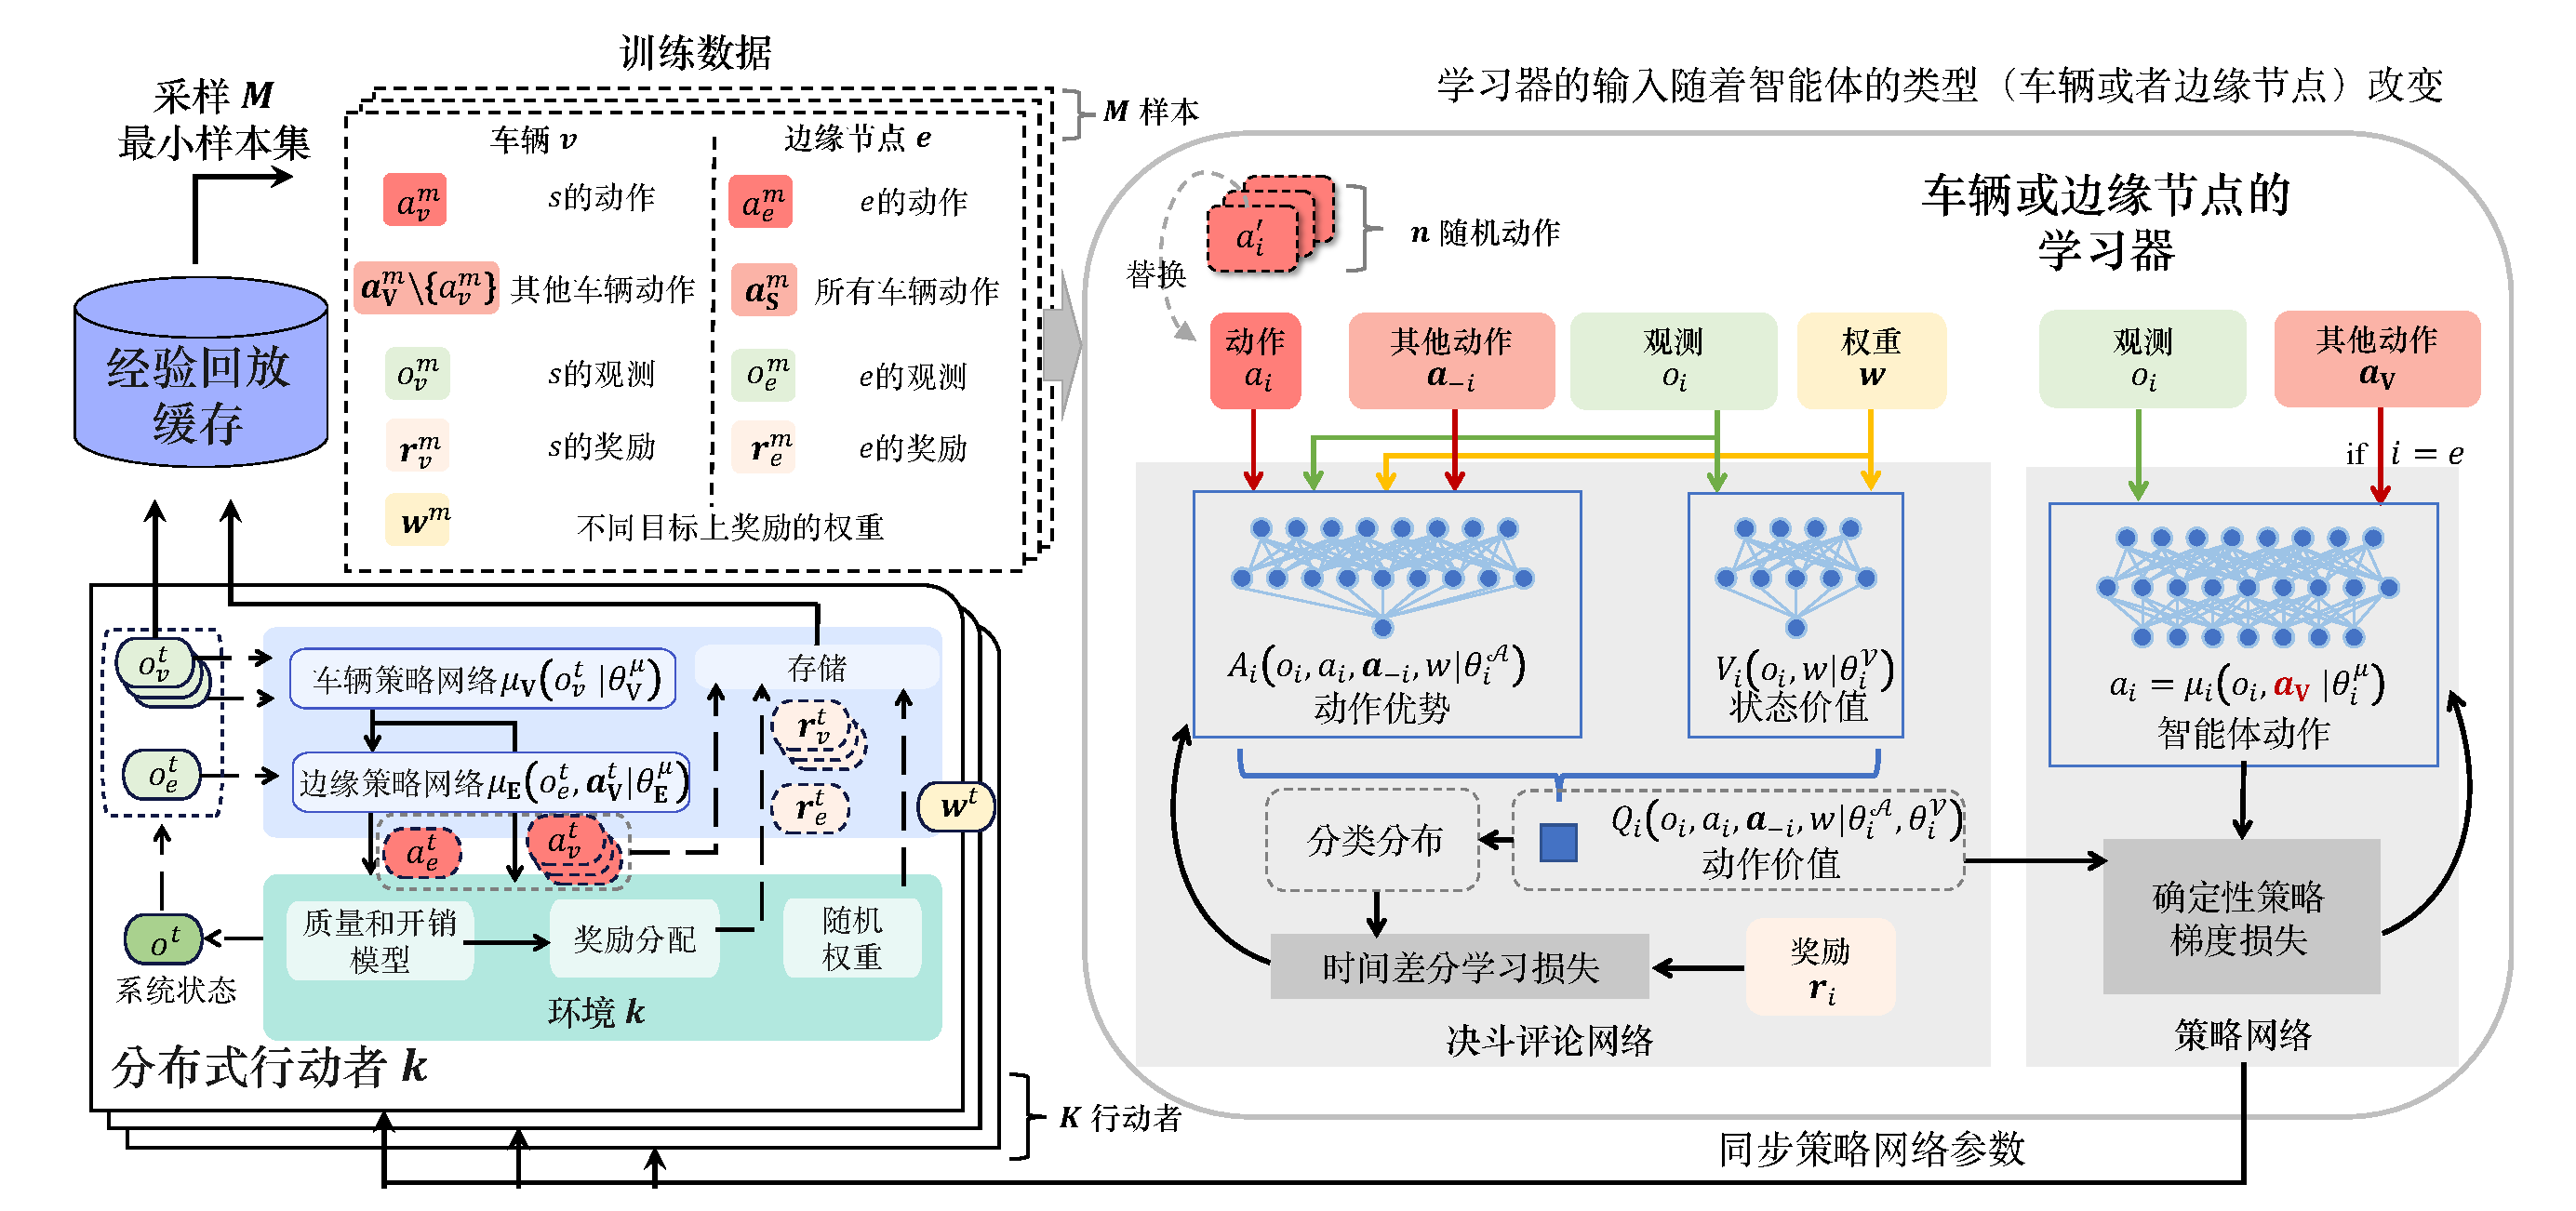
\includegraphics[width=0.65\textwidth]{fig/Fig4-2-solution-model.pdf}
\end{figure}
\end{textblock*}
\end{center}

\begin{center}
\begin{textblock*}{0.45\textwidth}(0.5cm,1.8cm)
\begin{itemize}[itemsep=0.2\baselineskip] \englishfont 
	\item[\ding{111}] {\color{cqublue}{初始化}}
	\begin{itemize}[itemsep=0.2\baselineskip]
	\begin{small}
		\item[\ding{226}] 网络参数、经验回放缓存
	\end{small}
	\end{itemize}
	\item[\ding{111}] {\color{cqublue}{分布式策略执行}}
	\begin{itemize}[itemsep=0.2\baselineskip]
	\begin{small}
		\item[\ding{226}] $K$分布式行动者启动
		\item[\ding{226}] 独立与环境交互,并存储经验
		\item[\ding{226}] 交互过程将持续到学习器训练过程结束
	\end{small}
	\end{itemize}
	\item[\ding{111}] {\color{cqublue}{网络学习与更新}}
	\begin{itemize}[itemsep=0.2\baselineskip]
	\begin{small}
		\item[\ding{226}] 抽取小批量训练样本
		\item[\ding{226}] 评论家网络:基于分类分布的时间差分学习
		\item[\ding{226}] 策略网络:策略梯度
	\end{small}
	\end{itemize}
\end{itemize}
\end{textblock*}
\end{center}

\end{frame}

\begin{frame}
\frametitle{\englishfont \underline{算法}:MAMO模型}
\newBackground
\begin{center}
\begin{textblock*}{\textwidth}(4.5cm,2.6cm)
\begin{figure}
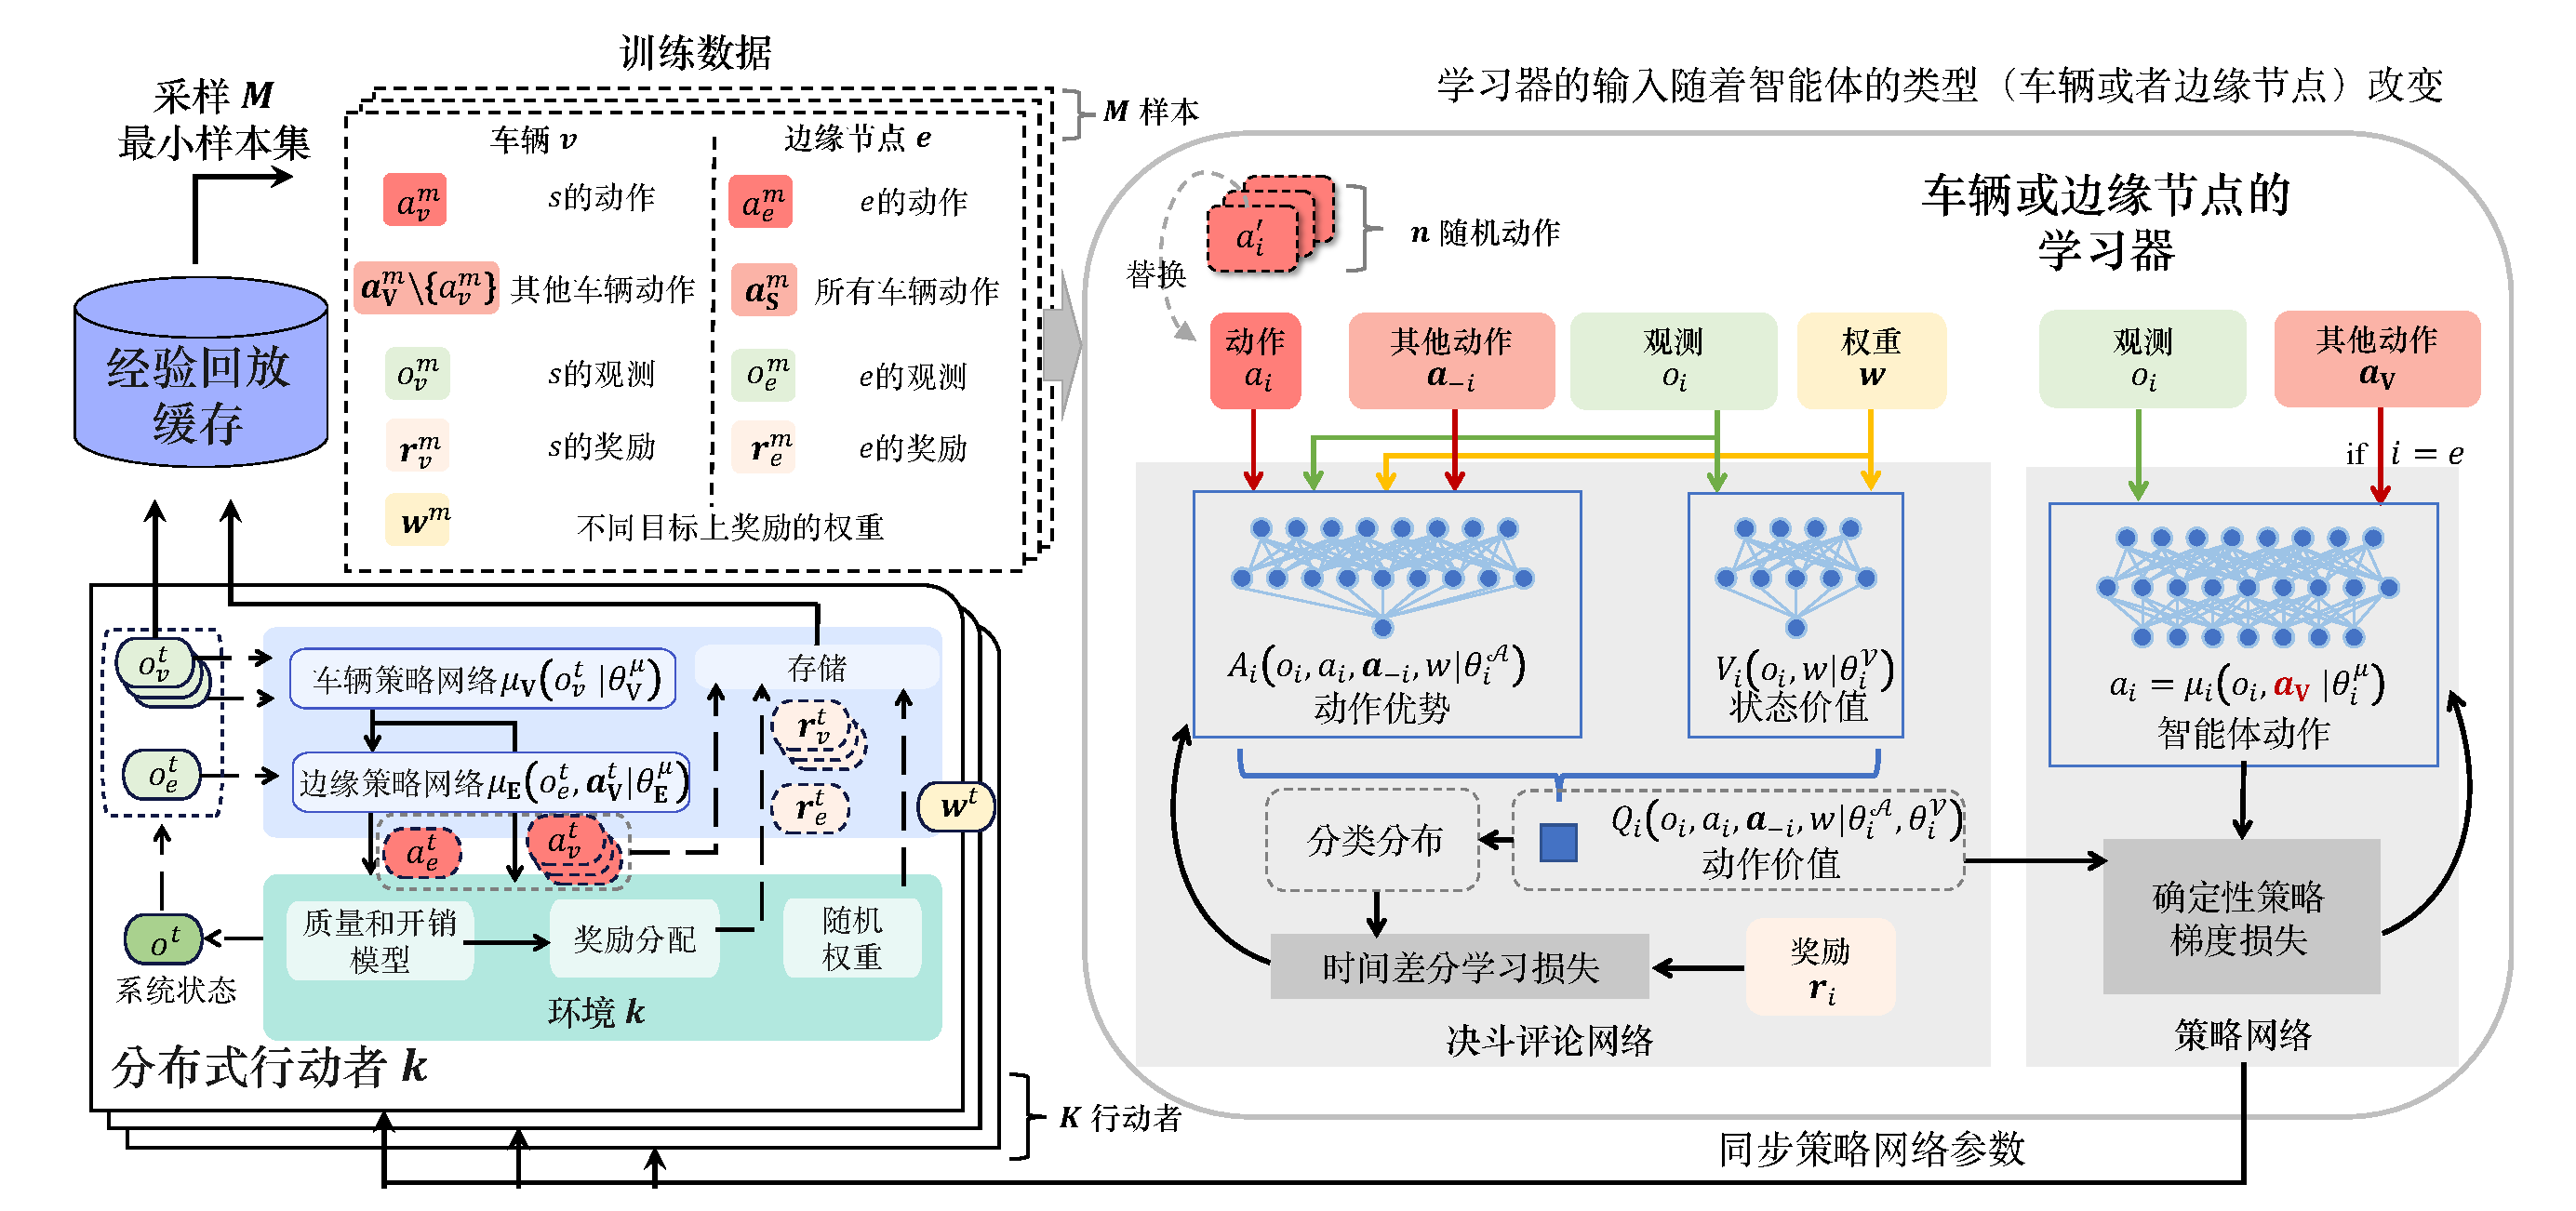
\includegraphics[width=0.65\textwidth]{fig/Fig4-2-solution-model.pdf}
\end{figure}
\end{textblock*}
\end{center}

\begin{center}
\begin{textblock*}{0.6\textwidth}(0.2cm,1.8cm)
\begin{itemize} \englishfont
	\item[\ding{111}] {\color{cqublue}{系统状态}}
	\item {\small{$\boldsymbol{o}_{v}^{t}=\left\{t, v, l_{v}^t, \mathbf{D}_{v}, \Phi_{v}, \mathbf{D}_{e}^{t}, \mathbf{D}_{\mathbf{I}_e^t}, \boldsymbol{w}^{t}\right\}$}}
	\item {\small{$\boldsymbol{o}_{e}^{t}=\left\{t, e, \operatorname{\mathbf{Dis}}_{\mathbf{V}, e}^{t}, \mathbf{D}_{1}, \ldots, \mathbf{D}_{V}, \mathbf{D}_{e}^{t}, \mathbf{D}_{\mathbf{I}_e^t}, \boldsymbol{w}^{t} \right\}$}}
	\item[\ding{111}] {\color{cqublue}{动作空间}}
	\item {\small{$\boldsymbol{a}_{v}^{t} = \{ \mathbf{C}_v^t,  \{ \lambda_{d, v}^{t}, p_{d, v}^{t} \mid \forall d \in \mathbf{D}_{v}^t \} , \pi_v^t   \}$}}
	\item {\small{$\boldsymbol{a}_{e}^{t} = \{b_{v, e}^{t} \mid \forall v \in \mathbf{V}_{e}^{t}\}$}}
	\item[\ding{111}] {\color{cqublue}{奖励函数}}
	\item {\small{$\boldsymbol{r}^{t} = \begin{bmatrix}  r^{(1)}\left(\boldsymbol{a}_{\mathbf{V}}^{t},\boldsymbol{a}_{e}^{t} \mid \boldsymbol{o}^{t}\right)  &  r^{(2)}\left(\boldsymbol{a}_{\mathbf{V}}^{t},\boldsymbol{a}_{e}^{t} \mid \boldsymbol{o}^{t}\right) \end{bmatrix} ^{T}$}}
	\item {\small{$r^{(1)}\left(\boldsymbol{a}_{\mathbf{V}}^{t},\boldsymbol{a}_{e}^{t} \mid \boldsymbol{o}^{t}\right)=\frac{1}{\left|\mathbf{I}_e^t\right|} \sum_{\forall i \in \mathbf{I}_e^t}\operatorname{QV}_{i}$}}
	\item {\small{$r^{(2)}\left(\boldsymbol{a}_{\mathbf{V}}^{t},\boldsymbol{a}_{e}^{t} \mid \boldsymbol{o}^{t}\right)=\frac{1}{\left|\mathbf{I}_e^t\right|} \sum_{\forall i \in \mathbf{I}_e^t} \operatorname{PV}_{j}$}}
\end{itemize}
\end{textblock*}
\end{center}
\end{frame}

\begin{frame}
\frametitle{\englishfont \underline{算法}:决斗评论家网络 (DCN)}
\newBackground
\begin{center}
\begin{textblock*}{\textwidth}(4.5cm,2.6cm)
\begin{figure}
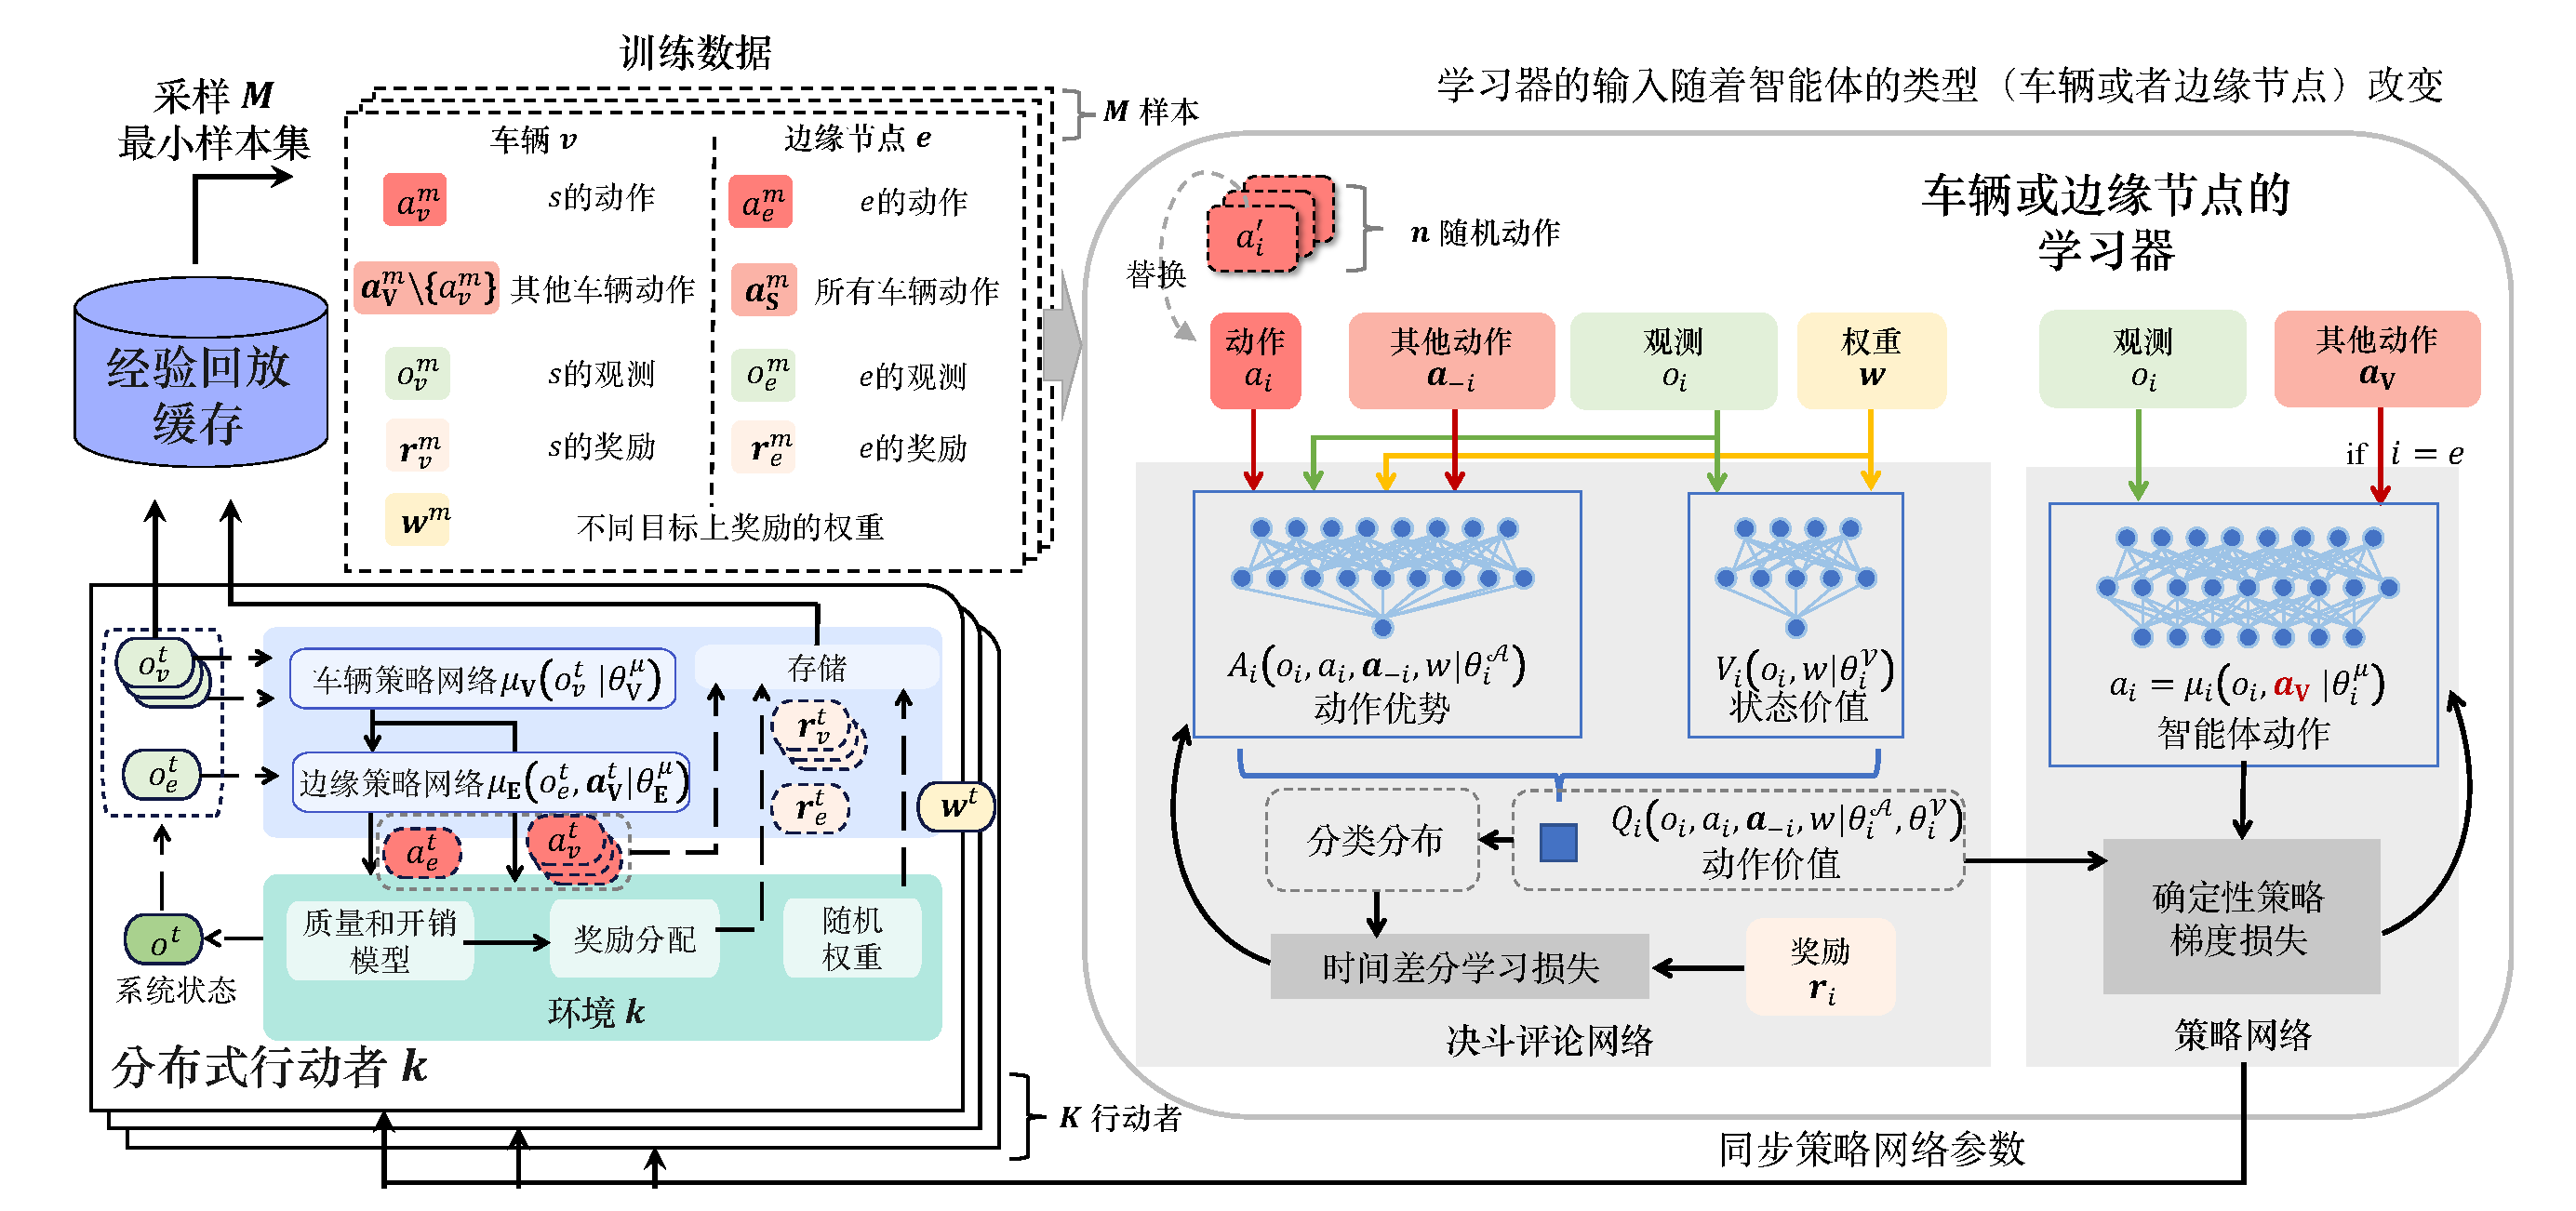
\includegraphics[width=0.65\textwidth]{fig/Fig4-2-solution-model.pdf}
\end{figure}
\end{textblock*}
\end{center}

\begin{center}
\begin{textblock*}{0.6\textwidth}(0.2cm,5.5cm)
\begin{align} \footnotesize
    & Q_{\mathbf{V}}\left({o}_{v}^{m}, {a}_{v}^{m}, \boldsymbol{a}_{\boldsymbol{\mathbf{V}}-v}^{m}, \boldsymbol{w}^{m} \mid \theta_{\mathbf{V}}^{Q} \right) \notag \\
    &= V_{\mathbf{V}}\left({o}_{v}^{m}, \boldsymbol{w}^{m} \mid \theta_{\mathbf{V}}^{\mathscr{V}} \right) + A_{\mathbf{V}}\left({o}_{v}^{m},  {a}_{v}^{m}, \boldsymbol{a}_{\boldsymbol{\mathbf{V}}-v}^{m}, \boldsymbol{w}^{m} \mid \theta_{\mathbf{V}}^{\mathscr{A}} \right) \notag \\
    &- \frac{1}{N} \sum_{\forall n} A_{\mathbf{V}}\left({o}_{v}^{m},  {a}_{v}^{m, n}, \boldsymbol{a}_{\boldsymbol{\mathbf{V}}-v}^{m}, \boldsymbol{w}^{m} \mid \theta_{\mathbf{V}}^{\mathscr{A}} \right) \notag
\end{align}

\end{textblock*}
\end{center}

\begin{center}
\begin{textblock*}{0.6\textwidth}(0.2cm,1.8cm)
\begin{itemize} \englishfont
	\item[\ding{111}] {\color{cqublue}{动作优势网络 (AA)}}
	\item 车辆 {\small{$A_{\mathbf{V}}\left({o}_{v}^{m},  {a}_{v}^{m}, \boldsymbol{a}_{\boldsymbol{\mathbf{V}}-v}^{m}, \boldsymbol{w}^{m} \mid \theta_{\mathbf{V}}^{\mathscr{A}} \right)$}}
	\item 边缘节点 {\small{$A_{\mathbf{E}}\left({o}_{e}^{m},  {a}_{e}^{m}, \boldsymbol{a}_{\boldsymbol{\mathbf{V}}}^{m}, \boldsymbol{w}^{m} \mid \theta_{\mathbf{E}}^{\mathscr{A}} \right)$}}
	\item[\ding{111}] {\color{cqublue}{状态价值网络 (SV)}}
	\item 车辆 {\small{$V_{\mathbf{V}}\left({o}_{v}^{m}, \boldsymbol{w}^{m} \mid \theta_{\mathbf{V}}^{\mathscr{V}} \right)$}}
	\item 边缘节点 {\small{$V_{\mathbf{E}}\left({o}_{e}^{m}, \boldsymbol{w}^{m} \mid \theta_{\mathbf{E}}^{\mathscr{V}} \right)$}}
	\item[\ding{111}] {\color{cqublue}{动作价值}}
	\item 
\end{itemize}
\end{textblock*}
\end{center}
\end{frame}

\begin{frame}
\frametitle{\englishfont \underline{实验}:数据与基本设置}
\newBackground

\begin{center}
	\begin{textblock*}{\textwidth}(-3.2cm,2.3cm)
	\begin{table}[h] \englishfont
\resizebox{0.5\textwidth}{!}{%
\begin{tabular}{cc}
\toprule 
\textbf{参数} & \textbf{值}         \\ \midrule
最大传输功率        & 100 mW               \\
传输可靠性阈值       & 0.9           \\
及时性加权系数          & 0.6              \\
一致性加权系数 & 0.4\\
冗余度加权系数 & 0.2 \\
感知开销加权系数         & 0.4  \\
传输开销加权系数         & 0.4  \\
策略网络        & 4 层全连接 (隐藏层 256-128)  \\
评论家网络         & 4 层全连接 (隐藏层 512-256) \\
学习率         & 1$\times10^{-4}$              \\
折扣因子        & 0.996              \\
经验回放缓存大小    & 1$\times10^{6}$          \\
批大小         & 256                \\ \bottomrule
\end{tabular}%
}
\end{table}
\end{textblock*}
\end{center}

\begin{center}
\begin{textblock*}{\textwidth}(0cm,1.8cm)
\begin{itemize} \englishfont
	\item[\ding{111}] {\color{cqublue}{实验与模型参数}}
\end{itemize}
\end{textblock*}
\end{center}

\begin{center}
\begin{textblock*}{0.65\textwidth}(7cm,1.8cm)
\begin{itemize}[itemsep=0.2\baselineskip]  \englishfont 
	\item[\ding{111}] {\color{cqublue}{对比算法}}
	\begin{itemize}[itemsep=0.2\baselineskip] 
	\begin{small}
		\item[\ding{226}] 随机分配 ({\color{red}{RA}})
		\item[\ding{226}] 分布式深度确定性策略梯度 ({\color{red}{D4PG}})
		\item[\ding{226}] 多智能体分布式深度确定性策略梯度 ({\color{red}{MAD4PG}})
		\item
	\end{small}
	\end{itemize}
\end{itemize}
\end{textblock*}
\end{center}

\begin{center}
\begin{textblock*}{0.65\textwidth}(7cm,3.85cm)
\begin{itemize}[itemsep=0.2\baselineskip] \englishfont
	\item[\ding{111}] {\color{cqublue}{性能评估指标}}
	\begin{itemize}[itemsep=0.2\baselineskip]
	\begin{small}
		\item[\ding{226}] 单位开销质量 ({\color{red}{QPUC}})\\
		{\small{$\operatorname{QPUC}=\frac{\sum_{\forall t \in \mathbf{T}} \sum_{\forall e \in \mathbf{E}} \sum_{\forall i \in \mathbf{I}_e^t} \mathrm{QV}_i}{\sum_{\forall t \in \mathbf{T}} \sum_{\forall e \in \mathbf{E}} \sum_{\forall i \in \mathbf{I}_e^t} \mathrm{CV}_i}$}}
		\item[\ding{226}] 单位质量利润 ({\color{red}{PPUQ}})\\
		{\small{$\operatorname{PPUQ}=\frac{\sum_{\forall t \in \mathbf{T}} \sum_{\forall e \in \mathbf{E}} \sum_{\forall i \in \mathbf{I}_e^t}\mathrm{PV}_i}{\sum_{\forall t \in \mathbf{T}} \sum_{\forall e \in \mathbf{E}} \sum_{\forall i \in \mathbf{I}_e^t} \mathrm{QV}_i}$}}
		\item[\ding{226}] 平均及时性 ({\color{red}{AT}}) \hspace{1em}平均冗余度 ({\color{red}{AR}})
		\item [\ding{226}] 平均感知开销({\color{red}{ASC}}) \hspace{1em}平均传输开销({\color{red}{ATC}})
	\end{small}
	\end{itemize}
\end{itemize}
\end{textblock*}
\end{center}

\end{frame}

\begin{frame}
\newBackground

\begin{overlayarea}{\textwidth}{3cm}
\only<1-1>{
\frametitle{\englishfont \underline{实验}:算法收敛性}
\begin{center} \englishfont \footnotesize
\begin{textblock*}{\textwidth}(1cm,2.2cm)
	\begin{figure}
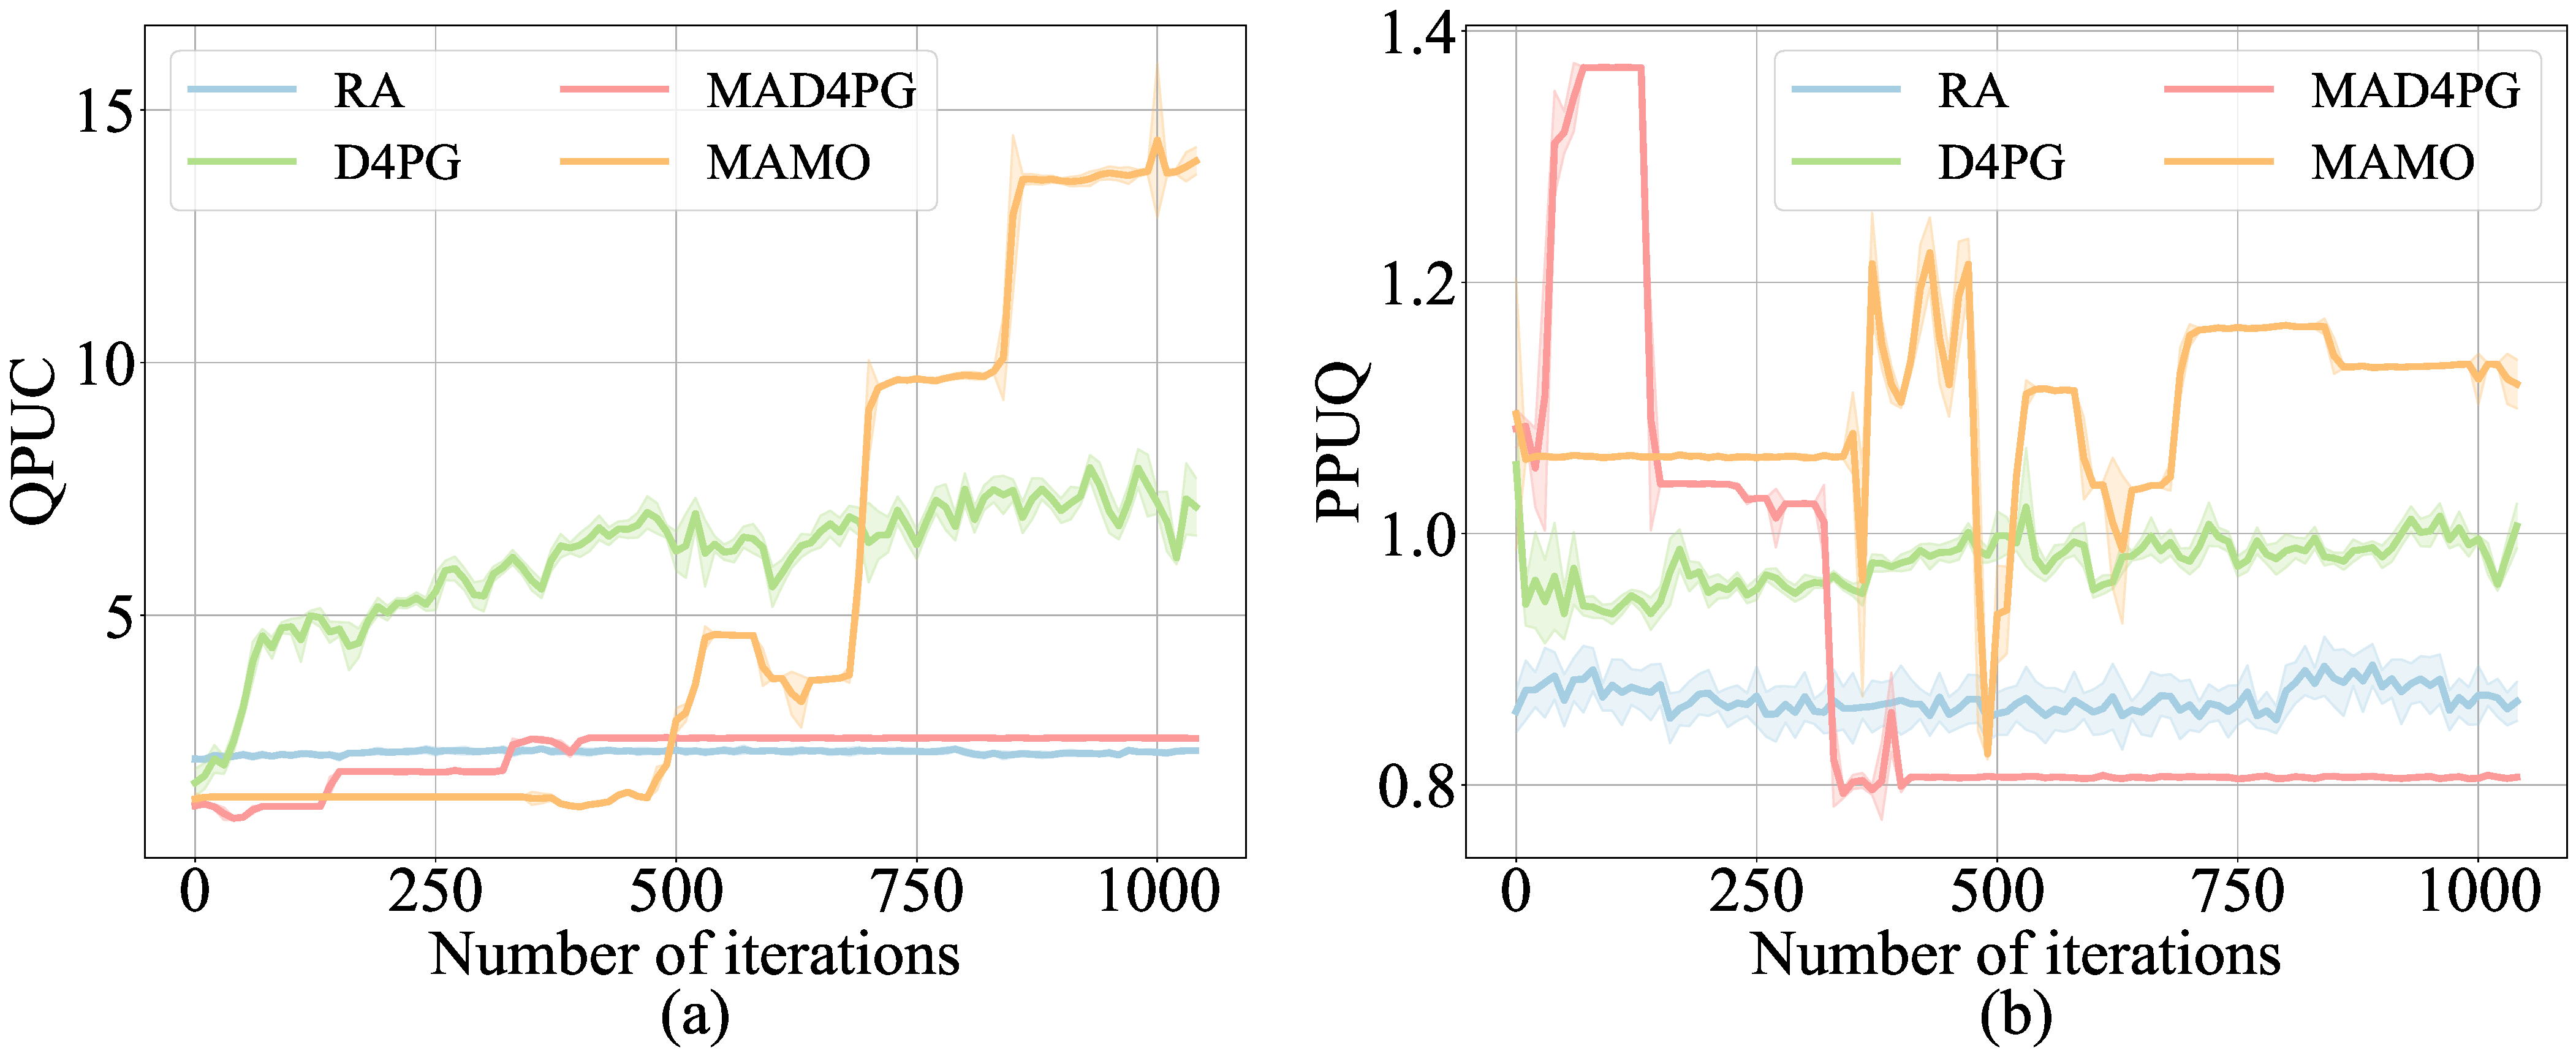
\includegraphics[width=1\textwidth]{fig/Fig4-3-different-algorithms.pdf}
	\end{figure}
\end{textblock*}
\end{center}
}

\only<2-2>{
\frametitle{\englishfont \underline{实验}:算法收敛性}
\begin{center} \englishfont \footnotesize
\begin{textblock*}{\textwidth}(1cm,2.2cm)
	\begin{figure}
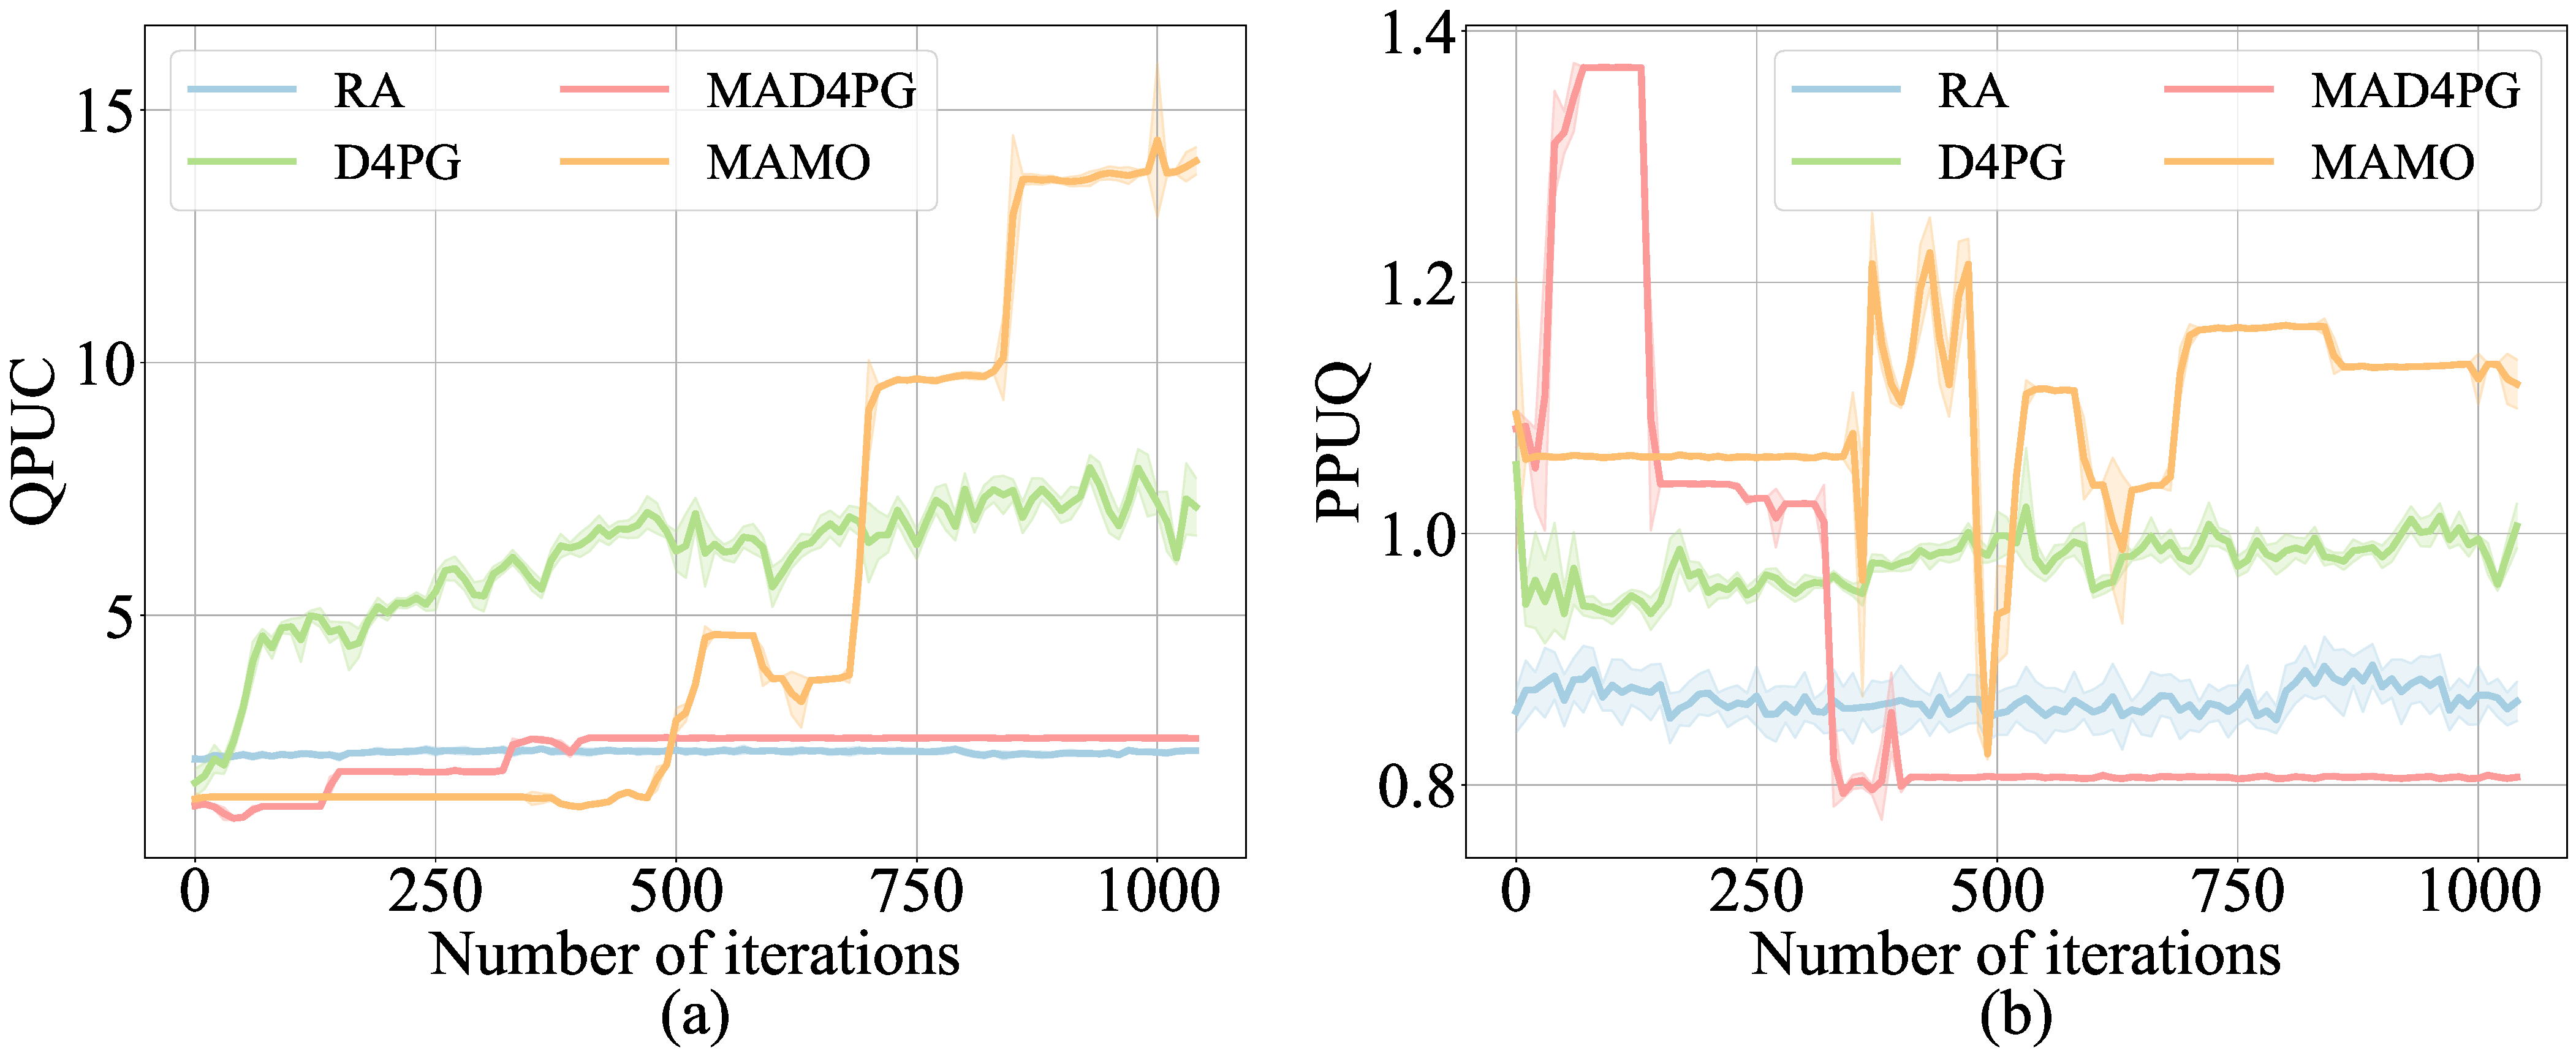
\includegraphics[width=1\textwidth]{fig/Fig4-3-different-algorithms.pdf}
	\end{figure}
\end{textblock*}
\end{center}
}

\only<2-2>{
\begin{center} \englishfont \footnotesize
\begin{textblock*}{\textwidth}(0cm,2.55cm)
{\Huge{\color{red}\ding{216}}}
\end{textblock*}
\end{center}

\begin{center} \englishfont \footnotesize
\begin{textblock*}{\textwidth}(6.95cm,3.5cm)
{\Huge{\color{red}\ding{216}}}
\end{textblock*}
\end{center}
}

\only<3-3>{
\frametitle{\englishfont \underline{实验}:神经元数量的影响}
\begin{center} \englishfont \footnotesize
\begin{textblock*}{\textwidth}(1cm,2.2cm)
	\begin{figure}
\includegraphics[width=1\textwidth]{fig/Fig4-4-different-networks.pdf}
	\end{figure}
\end{textblock*}
\end{center}
}

\only<4-4>{
\frametitle{\englishfont \underline{实验}:神经元数量的影响}
\begin{center} \englishfont \footnotesize
\begin{textblock*}{\textwidth}(1cm,2.2cm)
	\begin{figure}
\includegraphics[width=1\textwidth]{fig/Fig4-4-different-networks.pdf}
	\end{figure}
\end{textblock*}
\end{center}
}

\only<4-4>{
\begin{center} \englishfont \footnotesize
\begin{textblock*}{\textwidth}(-2.45cm,1.9cm)
{\Huge{\color{red}\ding{216}}}
\end{textblock*}
\end{center}

\begin{center} \englishfont \footnotesize
\begin{textblock*}{\textwidth}(4.7cm,5.3cm)
{\Huge{\color{red}\ding{216}}}
\end{textblock*}
\end{center}

}

\only<5-5>{
\frametitle{\englishfont \underline{实验}:交通场景的影响}
\begin{center} \englishfont \footnotesize
\begin{textblock*}{\textwidth}(1cm,1.8cm)
	\begin{figure}
\includegraphics[width=0.55\textwidth]{fig/Fig4-5-different-scenarios.pdf}
	\end{figure}
\end{textblock*}
\end{center}
}

\only<6-6>{
\frametitle{\englishfont \underline{实验}:交通场景的影响}
\begin{center} \englishfont \footnotesize
\begin{textblock*}{\textwidth}(1cm,1.8cm)
	\begin{figure}
\includegraphics[width=0.55\textwidth]{fig/Fig4-5-different-scenarios.pdf}
	\end{figure}
\end{textblock*}
\end{center}
}

\only<6-6>{

\begin{center} \englishfont \footnotesize
\begin{textblock*}{\textwidth}(-1.75cm,1.6cm)
{\LARGE{\color{red}\ding{216}}}
\end{textblock*}
\end{center}

\begin{center} \englishfont \footnotesize
\begin{textblock*}{\textwidth}(2.2cm,1.6cm)
{\LARGE{\color{red}\ding{216}}}
\end{textblock*}
\end{center}

\begin{center} \englishfont \footnotesize
\begin{textblock*}{\textwidth}(2.2cm,6.85cm)
{\LARGE{\color{red}\ding{216}}}
\end{textblock*}
\end{center}

\begin{center} \englishfont \footnotesize
\begin{textblock*}{\textwidth}(-1.75cm,6.8cm)
{\LARGE{\color{red}\ding{216}}}
\end{textblock*}
\end{center}
}

\only<7-7>{
\frametitle{\englishfont \underline{实验}:V2I带宽的影响}
\begin{center} \englishfont \footnotesize
\begin{textblock*}{\textwidth}(1cm,1.8cm)
	\begin{figure}
\includegraphics[width=0.9\textwidth]{fig/Fig4-6-different-bandwidths.pdf}
	\end{figure}
\end{textblock*}
\end{center}
}

\only<8-8>{
\frametitle{\englishfont \underline{实验}:V2I带宽的影响}
\begin{center} \englishfont \footnotesize
\begin{textblock*}{\textwidth}(1cm,1.8cm)
	\begin{figure}
\includegraphics[width=0.9\textwidth]{fig/Fig4-6-different-bandwidths.pdf}
	\end{figure}
\end{textblock*}
\end{center}
}

\only<8-8>{
\begin{center} \englishfont \footnotesize
\begin{textblock*}{\textwidth}(-3.3cm,2.5cm)
{\LARGE{\color{red}\ding{216}}}
\end{textblock*}
\end{center}

\begin{center} \englishfont \footnotesize
\begin{textblock*}{\textwidth}(1cm,1.65cm)
{\LARGE{\color{red}\ding{216}}}
\end{textblock*}
\end{center}

\begin{center} \englishfont \footnotesize
\begin{textblock*}{\textwidth}(5.2cm,3.3cm)
{\LARGE{\color{red}\ding{216}}}
\end{textblock*}
\end{center}

\begin{center} \englishfont \footnotesize
\begin{textblock*}{\textwidth}(-2.7cm,6.8cm)
{\LARGE{\color{red}\ding{216}}}
\end{textblock*}
\end{center}

\begin{center} \englishfont \footnotesize
\begin{textblock*}{\textwidth}(0.65cm,6.46cm)
{\LARGE{\color{red}\ding{216}}}
\end{textblock*}
\end{center}

\begin{center} \englishfont \footnotesize
\begin{textblock*}{\textwidth}(5.65cm,6.65cm)
{\LARGE{\color{red}\ding{216}}}
\end{textblock*}
\end{center}
}

\only<9-9>{
\frametitle{\englishfont \underline{实验}:视图需求的影响}
\begin{center} \englishfont \footnotesize
\begin{textblock*}{\textwidth}(1cm,1.8cm)
	\begin{figure}
\includegraphics[width=0.9\textwidth]{fig/Fig4-7-different-numbers.pdf}
	\end{figure}
\end{textblock*}
\end{center}
}

\only<10-10>{
\frametitle{\englishfont \underline{实验}:视图需求的影响}
\begin{center} \englishfont \footnotesize
\begin{textblock*}{\textwidth}(1cm,1.8cm)
	\begin{figure}
\includegraphics[width=0.9\textwidth]{fig/Fig4-7-different-numbers.pdf}
	\end{figure}
\end{textblock*}
\end{center}
}

\only<10-10>{
\begin{center} \englishfont \footnotesize
\begin{textblock*}{\textwidth}(-4.3cm,1.8cm)
{\LARGE{\color{red}\ding{216}}}
\end{textblock*}
\end{center}

\begin{center} \englishfont \footnotesize
\begin{textblock*}{\textwidth}(0cm,1.75cm)
{\LARGE{\color{red}\ding{216}}}
\end{textblock*}
\end{center}

\begin{center} \englishfont \footnotesize
\begin{textblock*}{\textwidth}(5.2cm,3.45cm)
{\LARGE{\color{red}\ding{216}}}
\end{textblock*}
\end{center}

\begin{center} \englishfont \footnotesize
\begin{textblock*}{\textwidth}(-2.7cm,6.8cm)
{\LARGE{\color{red}\ding{216}}}
\end{textblock*}
\end{center}

\begin{center} \englishfont \footnotesize
\begin{textblock*}{\textwidth}(0.65cm,6.65cm)
{\LARGE{\color{red}\ding{216}}}
\end{textblock*}
\end{center}

\begin{center} \englishfont \footnotesize
\begin{textblock*}{\textwidth}(5.65cm,6.65cm)
{\LARGE{\color{red}\ding{216}}}
\end{textblock*}
\end{center}
}
\end{overlayarea}
\end{frame}

\subsection[\englishfont 2.4 超视距碰撞预警原型系统设计及实现]{2.4 超视距碰撞预警原型系统设计及实现}

\begin{frame}
\frametitle{\englishfont 研究贡献}
\newBackground
\begin{center}
\begin{textblock*}{\textwidth}(-2cm,1.8cm)
\begin{spacing}{0}
  \small \englishfont \colorbox{cqublue}{\color{white}{原型系统的设计和实现是针对VCPS必要的{\color{yellow}{验证手段}}}}
\end{spacing}
\end{textblock*}
\end{center}

\begin{center}
\begin{textblock*}{\textwidth}(-1.8cm,2.8cm)
\begin{minipage}[t]{0.7\textwidth}
\begin{itemize}[itemsep=0.2\baselineskip] \englishfont 
	\item[\ding{111}] {{\color{cqublue}{\textbf{算法}}}:基于VCPS优化的碰撞预警} 
	\begin{itemize}[itemsep=0.2\baselineskip]
	\begin{small}
		\item[\ding{226}] 基于稳定分布的V2I应用层传输时延拟合模型
		\item[\ding{226}] 基于车辆轨迹和历史信息的丢包检测机制
	\end{small}
	\end{itemize}
	\item[\ding{111}]  {{\color{cqublue}{\textbf{系统}}}:超视距碰撞预警{\color{red}{原型系统}}}
	\begin{itemize}
	\begin{small}
		\item[\ding{226}] 基于C-V2X设备的硬件在环试验平台
		\item[\ding{226}] 原型系统实现
	\end{small}
	\end{itemize}
\end{itemize}
\end{minipage}
\end{textblock*}
\end{center}

\begin{center}
\begin{textblock*}{\textwidth}(-2cm,6.5cm)
\fbox{\begin{minipage}[t]{0.65\textwidth}\englishfont \tiny [6] \underline{\textcolor{cqublue}{XU X}}, LIU K, XIAO K, et al. \textcolor{cqublue}{Vehicular fog computing enabled real-time collision warning via trajectory calibration}[J]. Mobile Networks and Applications (\textcolor{red}{MONET}), 2020, 25(6): 2482-2494. 影响因子: 3.077(2021), 2.92(5年) (中科院SCI 3区)
\end{minipage}}
\fbox{\begin{minipage}[t]{0.65\textwidth}\englishfont \tiny [7] \underline{\textcolor{cqublue}{XU X}}, LIU K, XIAO K, et al. \textcolor{cqublue}{Design and implementation of a fog computing based collision warning system in VANETs}[C]. IEEE ISPCE-CN, 2018. (最佳论文奖)
\end{minipage}}
\end{textblock*}
\end{center}

\begin{center}
\begin{textblock*}{\textwidth}(6cm,1.8cm)
\begin{figure}
\includegraphics[width=0.4\textwidth]{fig/Fig5-1-example.pdf}
\end{figure}
\begin{figure}
\includegraphics[width=0.4\textwidth]{fig/Fig5-12-2.pdf}
\end{figure}
\end{textblock*}
\end{center}
\end{frame}

\begin{frame}
\frametitle{\englishfont \underline{算法}:流程}
\newBackground

\begin{center}
\begin{textblock*}{1\textwidth}(0.5cm,1.8cm)
\begin{itemize}[itemsep=0.2\baselineskip] \englishfont
\item[\ding{111}] {\color{cqublue}{车辆状态更新}}
	\begin{itemize}[itemsep=0.2\baselineskip]
	\begin{small}
		\item[\ding{226}] 基于V2I传输时延拟合模型估计传输时延
		\item[\ding{226}] 根据车辆速度和加速度更新其实时状态
	\end{small}
	\end{itemize}	
\item[\ding{111}] {\color{cqublue}{丢包检测}}
	\begin{itemize}[itemsep=0.2\baselineskip]
	\begin{small}
		\item[\ding{226}] 根据历史位置判断车辆是否在通信范围内
		\item[\ding{226}] 在通信范围内却未收到数据包,则认为已丢失
		\item[\ding{226}] 丢失的数据包使用历史记录更新它们的状态
	\end{small}
	\end{itemize}
	\item[\ding{111}] {\color{cqublue}{轨迹预测}}
	\begin{itemize}[itemsep=0.2\baselineskip]
	\begin{small}
		\item[\ding{226}] 基于修正的视图预测所有车辆未来的轨迹
	\end{small}
	\end{itemize}
	\item[\ding{111}] {\color{cqublue}{碰撞预警}}
	\begin{itemize}[itemsep=0.2\baselineskip]
	\begin{small}
		\item[\ding{226}] 计算每对车辆的车头时距
		\item[\ding{226}]通过车头时距阈值来检测潜在碰撞
	\end{small}
	\end{itemize}
\end{itemize}
\end{textblock*}
\end{center}

\begin{center}
\begin{textblock*}{\textwidth}(5.2cm,2.6cm)
\begin{figure}
\includegraphics[width=0.45\textwidth]{fig/Fig5-1-example.pdf}
\end{figure}
\end{textblock*}
\end{center}

\end{frame}

\begin{frame}
\frametitle{\englishfont \underline{算法}:V2I应用层时延拟合模型}
\newBackground

\begin{center}
\begin{textblock*}{0.7\textwidth}(0cm,4.2cm)
	\scriptsize
	\begin{numcases}{E \exp (i t X)=}
\exp \left\{-\sigma^{\alpha}|t|^{\alpha}[1-i \beta \tan (\alpha \pi / 2) \operatorname{sgn}(t)]+i \mu t\right\}, &$\alpha \neq 1$ \notag \\
\exp \{-\sigma|t[1+i \beta(2 / \pi) \operatorname{sgn}(t) \ln (|t|)]+i \mu t\},  &$\alpha=1$ \notag
\end{numcases}
\end{textblock*}
\end{center}

\begin{center}
\begin{textblock*}{0.7\textwidth}(0.5cm,1.8cm)
\begin{itemize}[itemsep=0.2\baselineskip] \englishfont 
	\item[\ding{111}]  {\color{cqublue}{数据}}
	\begin{itemize}[itemsep=0.2\baselineskip]
	\begin{small}
		\item[\ding{226}] 现场测试得到传输时延数据
		\item[\ding{226}] 分布不服从高斯分布
	\end{small} 
	\end{itemize}
	\item[\ding{111}]  {\color{cqublue}{稳定分布}}
	\begin{itemize}[itemsep=0.2\baselineskip]
	\begin{small}
		\item[\ding{226}] 适用于对非高斯过程进行估计
		\item
		\item
	\end{small} 
	\end{itemize}
	\item[\ding{111}]  {\color{cqublue}{拟合结果}}
	\begin{itemize}[itemsep=0.2\baselineskip]
	\begin{small}
	\item[\ding{226}] 几乎是对称的 ($\alpha = 1.77395$)
	\item[\ding{226}] 围绕均值 ($\mu = 72.7343$)
	\item[\ding{226}] 分布具有左偏度 ($\beta = 1$)
	\item[\ding{226}] 与均值的离散程度较大 ($\sigma = 13.3685$)
	\end{small} 
	\end{itemize}
\end{itemize}
\end{textblock*}
\end{center}

\begin{center}
\begin{textblock*}{\textwidth}(5.8cm,2.6cm)
\begin{figure}
\includegraphics[width=0.43\textwidth]{fig/Fig5-3-delay-fitting.pdf}
\end{figure}
\end{textblock*}
\end{center}

\end{frame}


\begin{frame}
\frametitle{\englishfont \underline{系统}:硬件在环平台框架}
\newBackground
\begin{center}
\begin{textblock*}{\textwidth}(5.3cm,2.5cm)
\begin{figure}
\includegraphics[width=0.5\textwidth]{fig/Fig5-8-hardware-in-the-loop-architecture.pdf}
\end{figure}
\end{textblock*}
\end{center}

\begin{center}
\begin{textblock*}{0.55\textwidth}(0.5cm,1.8cm)
\begin{itemize}[itemsep=0.2\baselineskip] \englishfont 
	\item[\ding{111}] {\color{cqublue}{硬件设备}}
	\begin{itemize}[itemsep=0.2\baselineskip]
	\begin{small}
		\item[\ding{226}] C-V2X 车载终端 (OBU)和路侧设备 (RSU)
		\item[\ding{226}] LTE-V2X PC5 和 5G UU 双模通信能力		
		\item[\ding{226}] 具有 GNSS 天线,可接收 GPS 卫星信号
	\end{small}
	\end{itemize}
	\item[\ding{111}] {\color{cqublue}{车端}}
	\begin{itemize}[itemsep=0.2\baselineskip]
	\begin{small}
		\item[\ding{226}] OBU 与平板电脑通过Wi-Fi 相互通信
		\item[\ding{226}] 平板电脑可作为车机界面进行碰撞预警消息的可视化
	\end{small}
	\end{itemize}
	\item[\ding{111}] {\color{cqublue}{边缘端}}
	\begin{itemize}[itemsep=0.2\baselineskip]
	\begin{small}
		\item[\ding{226}] PC 通过以太网与 RSU 相连
		\item[\ding{226}] PC 作为计算单元提供服务
	\end{small}
	\end{itemize}
\end{itemize}
\end{textblock*}
\end{center}
\end{frame}

\begin{frame}{基于 C-V2X 的硬件在环试验平台}
\newBackground
\begin{center}
\begin{textblock*}{\textwidth}(1cm,1.8cm)
\begin{figure}
\includegraphics[width=1\textwidth]{fig/Fig5-9-C-V2X-hardware-in-loop.pdf}
\end{figure}
\end{textblock*}
\end{center}
\end{frame}

\begin{frame}
\frametitle{\englishfont \underline{系统}:C-V2X 端到端时延}
\newBackground
\begin{center}
\begin{textblock*}{\textwidth}(5.2cm,2.2cm)
\begin{figure}
\includegraphics[width=0.5\textwidth]{fig/Fig5-10-delays.pdf}
\end{figure}
\end{textblock*}
\end{center}

\begin{center}
\begin{textblock*}{0.55\textwidth}(0.5cm,2.3cm)
\begin{itemize}[itemsep=0.2\baselineskip] \englishfont 
	\item[\ding{111}] {\color{cqublue}{数据包设置}}
	\begin{itemize}[itemsep=0.2\baselineskip]
	\begin{small}
		\item[\ding{226}] 以10 Hz的频率分别发送1000个数据包
		\item[\ding{226}] 大小从100 Bytes增加至7000 Bytes	
	\end{small}
	\end{itemize}
	\item[\ding{111}] {\color{cqublue}{时延结果分析}}
	\begin{itemize}[itemsep=0.2\baselineskip]
	\begin{small}
		\item[\ding{226}] 最小数据包 (100 Bytes)平均时延最短 (6.271 ms)
		\item[\ding{226}] 最大数据包 (7000 Bytes)平均时延最长 (9.570 ms)
	\end{small}
	\end{itemize}
\end{itemize}
\end{textblock*}
\end{center}

\end{frame}
\begin{frame}{超视距碰撞预警原型系统}
\frametitle{\englishfont \underline{系统}:超视距碰撞预警原型系统}
\newBackground
\includemedia[
    width=1\linewidth,
    height=0.45\linewidth,
    activate=pageopen,
    passcontext,
    addresource=/Users/neardws/Documents/My-Doctoral-Dissertation-Defense/fig/cws2/cws2.mp4,
    flashvars={
      source=/Users/neardws/Documents/My-Doctoral-Dissertation-Defense/fig/cws2/cws2.mp4
      &autoPlay=true
      &loop=true
    }
  ]{}{VPlayer.swf}
\end{frame}
\section[\englishfont 3 总结与展望]{总结与展望}
\begin{frame}{总结与展望} 
\newBackground
\begin{center}
\begin{textblock*}{1.2\textwidth}(1cm,2cm)
\begin{itemize}[itemsep=0.2\baselineskip]
 \englishfont
	\item[\ding{111}] {\color{cqublue}{工作总结}}
	\begin{itemize}[itemsep=0.2\baselineskip]
	\begin{small}
		\item[\ding{226}] \underline{架构}: 车联网分层服务架构,{\color{cqublue}{有机融合SDN与MEC}}
		\item[\ding{226}]  \underline{指标}: 车载信息物理融合质量指标,考虑{\color{cqublue}{时效性、完整性和一致性}}
		\item[\ding{226}] \underline{MADR算法}: 有效{\color{cqublue}{提高VCPS质量}}
		\item[\ding{226}] \underline{CRO问题}:协同传输与计算,以最大化任务完成率
		\item[\ding{226}] \underline{MAGT算法}:有效{\color{cqublue}{提高任务完成率}}
		\item[\ding{226}] \underline{双目标优化问题}:车载信息物理融合系统{\color{cqublue}{质量模型和开销模型}}
		\item[\ding{226}] \underline{MAMO算法}:有效实现{\color{cqublue}{质量和开销的均衡}}
	\end{small}
	\end{itemize}
	\item[\ding{111}]  {\color{cqublue}{研究展望}}
	\begin{itemize}[itemsep=0.2\baselineskip]
	\begin{small}
		\item[\ding{226}] 边缘节点之间的合作
		\item[\ding{226}] 车联网端边云架构,车辆、边缘节点和云协同
		\item 
	\end{small} 
	\end{itemize}
\end{itemize}
\end{textblock*}
\end{center}
\end{frame}

\section[\englishfont 4 研究成果总结]{研究成果总结}

\begin{frame}{论文发表}
\newBackground
\frametitle{论文发表 (第一作者或二作 (导师一作)\hspace{0.5em}\textcolor{red}{7}\hspace{0.5em}篇,另有\hspace{0.5em}\textcolor{red}{2}\hspace{0.5em}篇在投)}
\begin{center}
\begin{textblock*}{\textwidth}(-1.1cm,1.85cm)
\begin{minipage}[t]{0.83\textwidth}
\begin{itemize}
\setlength{\itemsep}{1pt}
\setlength{\parskip}{0pt}
\setlength{\parsep}{0pt}
	\begin{small}
	\item[1] \englishfont \underline{\textcolor{cqublue}{XU X}}, LIU K, DAI P, et al. Joint task offloading and resource optimization in NOMA-based vehicular edge computing: A game-theoretic DRL approach[J]. \textcolor{cqublue}{Journal of Systems Architecture} (\textcolor{red}{JSA}), 2023. (中科院SCI 2区)
	\item[2] \underline{\textcolor{cqublue}{许新操}}, 刘凯, 刘春晖, 等. 基于势博弈的车载边缘计算信道分配方法[J]. \textcolor{red}{电子学报}, 2021. (CCF T1类中文期刊)
	\item[3] \underline{\textcolor{cqublue}{XU X}}, LIU K, XIAO K, et al. Vehicular fog computing enabled real-time collision warning via trajectory calibration[J]. \textcolor{cqublue}{Mobile Networks and Applications} (\textcolor{red}{MONET}), 2020. (中科院SCI 3区)
	\item[4] LIU K, \underline{\textcolor{cqublue}{XU X}}, CHEN M, et al. A hierarchical architecture for the future Internet of Vehicles[J]. \textcolor{cqublue}{IEEE Communications Magazine} (\textcolor{red}{ComMag}), 2019. (中科院SCI 1区)
	\item[5] \underline{\textcolor{cqublue}{XU X}}, LIU K, ZHANG Q, et al. Age of view: A new metric for evaluating heterogeneous information fusion in vehicular cyber-physical systems[C]. \textcolor{red}{IEEE ITSC}, 2022. (智能交通领域重要会议)
	\item % 解决最后一个item行间距问题
	\end{small}
\end{itemize}
\end{minipage}
\end{textblock*}
\end{center}
\begin{center}
\begin{textblock*}{\textwidth}(7cm,1.85cm)
\begin{minipage}[t]{0.4\textwidth}
\begin{figure}
  \centering
  \includegraphics[width=0.65\textwidth]{fig/publication1.pdf}
\end{figure}
\end{minipage}
\end{textblock*}
\end{center}
\end{frame}

\begin{frame}{论文发表}
\newBackground
\frametitle{论文发表 (第一作者或二作 (导师一作)\hspace{0.5em}\textcolor{red}{7}\hspace{0.5em}篇,另有\hspace{0.5em}\textcolor{red}{2}\hspace{0.5em}篇在投)}
\begin{center}
\begin{textblock*}{\textwidth}(-2cm,1.85cm)
\begin{minipage}[t]{0.7\textwidth}
	\begin{itemize}
	\begin{small}
	\item[6] \englishfont \underline{\textcolor{cqublue}{许新操}}, 周易, 刘凯, 等. 车载雾计算环境中基于势博弈的分布式信道分配[C]. \textcolor{cqublue}{CWSN}, 2020. (最佳论文候选)
	\item[7] \underline{\textcolor{cqublue}{XU X}}, LIU K, XIAO K, et al. Design and implementation of a fog computing based collision warning system in VANETs[C]. \textcolor{cqublue}{IEEE ISPCE-CN}, 2018. (最佳论文奖)
	\item[8] \underline{\textcolor{cqublue}{XU X}}, LIU K, DAI P, et al. Cooperative sensing and heterogeneous information fusion in VCPS: A multi-agent deep reinforcement learning approach[J]. \textcolor{cqublue}{IEEE Transactions on Intelligent Transportation Systems} (\textcolor{red}{T-ITS}), under major revision. (中科院SCI 1区)
	\item[9] LIU K,\underline{\textcolor{cqublue}{XU X}}, DAI P, et al. Cooperative sensing and uploading for quality-cost tradeoff of digital twins in VEC[J]. \textcolor{cqublue}{IEEE Transactions on Consumer Electronics} (\textcolor{red}{TCE}), under minor revision. (中科院SCI 2区)
	\item % 解决最后一个item行间距问题
	\end{small}
\end{itemize}
\end{minipage}
\end{textblock*}
\end{center}

\begin{center}
\begin{textblock*}{\textwidth}(5.9cm,1.85cm)
\begin{minipage}[t]{0.4\textwidth}
\begin{figure}
  \centering
  \includegraphics[width=0.9\textwidth]{fig/publication2.pdf}
\end{figure}
\end{minipage}
\end{textblock*}
\end{center}

\end{frame}

\begin{frame}{论文发表}
\newBackground
\frametitle{论文发表 (合作作者\hspace{0.5em}\textcolor{red}{6}\hspace{0.5em}篇)}
\begin{center}
\begin{textblock*}{\textwidth}(1cm,1.85cm)
	\begin{footnotesize}
		\begin{itemize}
			\item[1] \englishfont LIU C, LIU K, REN H, \underline{\textcolor{cqublue}{XU X}}, et al. RtDS: Real-time distributed strategy for multi-period task offloading in vehicular edge computing environment[J]. \textcolor{cqublue}{Neural Computing and Applications}, to appear. (中科院SCI 2区)
			\item[2] XIAO K, LIU K, \underline{\textcolor{cqublue}{XU X}}, et al. Cooperative coding and caching scheduling via binary particle swarm optimization in software defined vehicular networks[J]. \textcolor{cqublue}{Neural Computing and Applications}, 2021. (中科院SCI 2区)
			\item[3] XIAO K, LIU K, \underline{\textcolor{cqublue}{XU X}}, et al. Efficient fog-assisted heterogeneous data services in software defined VANETs[J]. \textcolor{cqublue}{Journal of Ambient Intelligence and Humanized Computing}, 2021. (中科院SCI 3区)
			\item[4] LIU C, LIU K, \underline{\textcolor{cqublue}{XU X}}, et al. Real-time task offloading for data and computation intensive services in vehicular fog computing environments[C]. \textcolor{cqublue}{IEEE MSN}, 2020. (CCF C类国际会议)
			\item[5] ZHOU Y, LIU K, \underline{\textcolor{cqublue}{XU X}}, et al. Multi-period distributed delay-sensitive tasks offloading in a two-layer vehicular fog computing architecture[C]. \textcolor{cqublue}{NCAA}, 2020. (EI 索引)
			\item[6] ZHOU Y, LIU K, \underline{\textcolor{cqublue}{XU X}}, et al. Distributed scheduling for time-critical tasks in a two-layer vehicular fog computing architecture[C]. \textcolor{cqublue}{IEEE CCNC}, 2020. (EI 索引)
			\item % 解决最后一个item行间距问题
		\end{itemize}	
	\end{footnotesize}
\end{textblock*}
\end{center}
\end{frame}

\begin{frame}{代码开源}
\newBackground
\frametitle{\englishfont 代码开源 (获得 100+ GitHub Stars)}
\begin{minipage}[t]{0.6\textwidth}
	\begin{itemize}
		\begin{footnotesize}
			\item[1] 基于差分奖励的多智能体强化学习源代码\\ \href{https://github.com/neardws/Multi-Agent-Deep-Reinforcement-Learning}{\tiny \englishfont https://github.com/neardws/Multi-Agent-Deep-Reinforcement-Learning}
			\item[2] 基于博弈理论的多智能体强化学习源代码\\ \href{https://github.com/neardws/Game-Theoretic-Deep-Reinforcement-Learning}{\tiny \englishfont https://github.com/neardws/Game-Theoretic-Deep-Reinforcement-Learning}
			\item[3] 基于多目标的多智能体强化学习源代码\\ \href{https://github.com/neardws/MAMO-Deep-Reinforcement-Learning}{\tiny \englishfont https://github.com/neardws/MAMO-Deep-Reinforcement-Learning}
			\item[4] 基于视图校准的碰撞预警源代码\\ \href{https://github.com/neardws/fog-computing-based-collision-warning-system}{\tiny \englishfont https://github.com/neardws/fog-computing-based-collision-warning-system}
			\item[5] 基于C-V2X通信的碰撞预警原型系统实现源代码\\ \href{https://github.com/neardws/V2X-based-Collision-Warning}{\tiny \englishfont https://github.com/neardws/V2X-based-Collision-Warning}
			\item[6] 滴滴GAIA数据集处理源代码\\ \href{https://github.com/neardws/Vehicular-Trajectories-Processing-for-Didi-Open-Data}{\tiny \englishfont https://github.com/neardws/Vehicular-Trajectories-Processing-for-Didi-Open-Data}
			\item % 解决最后一个item行间距问题
		\end{footnotesize}
	\end{itemize}
\end{minipage}%
\begin{minipage}[t]{0.3\textwidth}
\begin{figure}
  \centering
  \includegraphics[width=1.2\textwidth]{fig/github_stars.pdf}
\end{figure}
\begin{figure}
  \centering
  \includegraphics[width=1\textwidth]{fig/github_gtdrl.pdf}
\end{figure}
\end{minipage}	
\end{frame}

\begin{frame}{科研项目与专利}
\newBackground
\begin{center}
\begin{textblock*}{\textwidth}(1cm,1.85cm)
\begin{itemize} \englishfont
	\item[\ding{111}] 参与科研项目
		\begin{itemize} 
		\begin{footnotesize}
			\item[\ding{226}] \textcolor{cqublue}{国家自然科学基金面上项目},“面向车联网边缘智能的计算模型部署与协同跨域优化”,项目编号: 62172064,2022/01–2025/12. (在研)
			\item[\ding{226}] \textcolor{cqublue}{国家自然科学基金面上项目},“面向大规模数据服务的异构融合车联网架构与协议研究”,项目编号: 61872049,2019/01–2022/12. (结题)
		\end{footnotesize}
		\end{itemize}
	\item[\ding{111}] 申请发明专利
		\begin{itemize}
		\begin{footnotesize}
			\item[\ding{226}] \underline{\textcolor{cqublue}{许新操}}, 刘凯, 李东. 一种针对软件定义车联网的控制平面视图构建方法. \textcolor{red}{已授权}. 专利号:ZL202110591822.1.
			\item[\ding{226}] 刘凯, 张浪, \underline{\textcolor{cqublue}{许新操}}, 任华玲, 周易. 一种基于边缘计算的盲区车辆碰撞预警方法. \textcolor{red}{已授权}. 专利号:ZL201910418745.2.
			\item[\ding{226}] 任华玲, 刘凯, 陈梦良, 周易, \underline{\textcolor{cqublue}{许新操}}. 一种基于雾计算的信息采集、计算、传输架构. \textcolor{red}{已授权}. 专利号:ZL201910146357.3.
		\end{footnotesize}
		\end{itemize}
	
\end{itemize}
\end{textblock*}
\end{center}
\end{frame}

\begin{frame}{盲审意见与修改情况}
\newBackground
\begin{center}
\begin{textblock*}{\textwidth}(1cm,1.85cm)
\begin{itemize}[itemsep=0.2\baselineskip] \englishfont
	\item[\ding{111}] \textcolor{cqublue}{总体评价 \textbf{A B B}}
	\item[\ding{111}] \textcolor{cqublue}{评审专家 1}
		\begin{itemize}[itemsep=0.2\baselineskip] 
		\begin{small}
			\item[\ding{52}] 车联网分层架构详细阐述
			\item[\ding{52}] VCPS质量定义增加实例
		\end{small}
		\end{itemize}
	\item[\ding{111}] \textcolor{cqublue}{评审专家 2}
		\begin{itemize}[itemsep=0.2\baselineskip] 
		\begin{small}
			\item[\ding{52}] 数据平面和控制平面概念介绍
			\item[\ding{52}] 论文符号定义优化
		\end{small}
		\end{itemize}
		\item[\ding{111}] \textcolor{cqublue}{评审专家 3}
		\begin{itemize}[itemsep=0.2\baselineskip] 
		\begin{small}
			\item[\ding{52}] 排版问题
			\item[\ding{52}] 碰撞预警系统图详细阐述
		\end{small}
		\end{itemize}
\end{itemize}
\end{textblock*}
\end{center}
\end{frame}

\begin{frame}
\newBackground
\Background
    \begin{center} \doublespacing
        {\Huge 致谢}\\
       	\textit{感谢刘凯教授多年的辛勤指导!}\\
       	\textit{感谢各位专家的指导!}\\
       	\textit{感谢所有给予我帮助的老师和同学!}
    \end{center}
\end{frame}

\begin{frame}
\newBackground
\Background
    \begin{center} \doublespacing
        {\Huge 敬请批评指正!}
    \end{center}
\end{frame}

\end{document}